%&pdflatex

\documentclass[12pt]{report}
\usepackage[a4paper]{geometry}
%\usepackage[left=3.5cm, right=2.5cm]{geometry} % margins

\usepackage{algorithm}
\usepackage{algpseudocode}
\usepackage{amsmath} % for implementation of the matrix environment
\usepackage{amssymb}
\usepackage{blindtext}
\usepackage{bm}
\usepackage{booktabs}
\usepackage{breakcites}
\usepackage{caption}
\usepackage[table]{xcolor}
\usepackage{color}
\usepackage[pdftex]{graphicx} \graphicspath{{./plots/}}
\usepackage[inline]{enumitem}
\usepackage{epstopdf} \epstopdfsetup{update} % only regenerate pdf files when eps file is newer
\usepackage{float} % figure groups aka floats
\usepackage{forest} % for MFS elimination tree diagram
\usepackage{gensymb}
\usepackage[shellescape,latex]{gmp} % metapost for UMLs
\usepackage[hidelinks]{hyperref} % ToC/LoA/LoF/LoT entries are links
% \usepackage{lscape}
\usepackage{pdflscape}
\usepackage{makecell}
\usepackage{mathptmx} % Times New Roman like font
\usepackage{pdfpages} % for inserting pdf as the initial pages
\usepackage{setspace} \onehalfspacing % 1.5 line spacing
\usepackage{subcaption}
\usepackage{xfrac} % nice slanted fractions
\usepackage{url}
\usepackage[utf8]{inputenc}

%\captionsetup[figure]{labelfont={bf}, textfont={small}}
%\captionsetup[subfigure]{labelfont={bf}, textfont={small}}

\newcommand{\bt}{\blindtext}
\newcommand{\eps}{\varepsilon}
%\newcommand{\rev}[1]{\textcolor{red}{#1}}
\newcommand{\rev}[1]{#1}
\newcommand{\T}[1]{\texttt{#1}}
\providecommand{\keywords}[1]{\textbf{Keywords:} \textit{#1}}

\algnewcommand\And{\,\textbf{and}\,}
\algnewcommand\Or{\,\textbf{or}\,}
\algnewcommand{\LineComment}[1]{\State \(\triangleright\) #1}
\renewcommand\theadalign{bl}

\definecolor{very-light-gray}{gray}{0.95}
\newcommand{\rowstripes}{\rowcolors{1}{white}{very-light-gray}}
\newcommand{\R}{\mathbb{R}}

\begin{document}


\includepdf[pages={-,{}}]{initial-pages.pdf} % `-' for all pages, `{}' for an empty page

\tableofcontents

($NO_2$)\chapter*{Abstract}\label{chap:abstract}
The city of Krakow (Poland) struggles with the problem of air pollution. This study attempts to verify if the selected statistical models - multiple linear regression, support vector regression and multilayer perceptron - could be applied to the problem of forecasting mean hourly PM2.5 concentrations 24 hours in advance. Tests were performed on data gathered by three monitoring stations during the 2014-2017 period. The models were found to be potentially useful with Root Mean Square Errors varying for winter from 43.912 to 55.634 $\mu g/m^3$, for spring - from 14.408 to 16.306 $\mu g/m^3$, for summer from 6.855 to 8.856 and for autumn from 21.768 to 25.870 $\mu g/m^3$. Their performance is, however, negatively impacted by difficulties with predicting pollution level spikes.

\subsection*{Keywords}
\textit{air quality \quad air pollution \quad PM2.5 \quad forecast \quad machine learning \quad neural networks}

\part{Introduction}
\chapter{Introduction}\label{chap:introduction}

\section{Motivation}
Krakow is one of the major Polish cities located in the Lesser Poland region in the southern part of the country. Due to its unfavourable topographical conditions (the city lies in the valley of the Vistula river) and the density of buildings reducing the air flow it struggles with rather severe air pollution.
\\\\
One of the more common pollutants that can be found in the city is particulate matter. In practice its concentrations are usually registered for its two types: PM2.5 and PM10, which denote airborne particles with diameters under 2.5 $\mu m$ and 10 $\mu m$ accordingly. In order to illustrate the scale of the problem it is worth noting that in the database published by the World Health Organisation in 2016 \cite{WHO2016AMBIENT} containing mean annual PM2.5 and PM10 concentrations in 1712 cities located in Europe (including Turkey), Krakow was ranked $55^{th} (37 \mu / m^3)$ and $74^{th} (51 \mu g / m^3)$, accordingly. Maximum mean annual concentrations recommended by the WHO are 10 $\mu g / m^3$ for PM2.5 and 20 $\mu g / m^3$ for PM10 \cite{WHO2008AQGUIDELINES}.
\\\\
The problem of poor air quality is especially prevalent during the heating season which spans roughly from the mid September to the beginning of April. During that period it is fairly common to observe in Krakow considerable exceedances of daily mean PM concentration limits. For example there are cases, when the maximum hourly PM10 concentrations reach levels above 200 $\mu g / m^3$ \cite{WIOSALERTS}, while the mean daily limit recommended by the Regional Inspectorate of Environmental Protection is 50 $\mu g / m^3$ \cite{WIOSNORMS}. One of the major causes of such high levels of pollution during winter is the fact that coal burning stoves are still popular among the residents of Krakow and nearby villages. According to the results of stocktaking of coal burners, commissioned by the city council and finished in 2015, there were approximately 24 thousand such stoves. It is assumed that since then more than 6 thousand of them have been liquidated \cite{COALBURNERS}, however the number of remaining ones is still considerable.
\\\\
Poor quality of air constitutes a serious problem for the residents of Krakow, given the harmful influence of pollutants on their health. According to the World Health Organisation prolonged exposure to high concentrations of particulate matter might cause increased morbidity from cardiovascular and respiratory diseases (e.g. asthma) as well as increased cardiopulmonary and lung cancer mortality and, as a result, reduced life expectancy \cite{WHO2013PMHEALTH}.
\\\\
Finding a reliable way of predicting PM2.5 concentrations in advance, while not solving the problem completely, could be beneficial for the residents, as it would allow to warn them about the incoming high pollution episodes. Potentially, it would be helpful not only for individuals but also for the local authorities, who could, for example, organise a day of free public transport in order to lower the production of exhaust fumes.

\section{Research goal} \label{sec:introduction-research-goal}
The problem of air pollution is common to many cities throughout the globe. Because of that, multiple attempts have been made to create predictive models which could be used for warning residents about the possible threats of high pollution levels, some of which were quite successful (for example \cite{VLACHOGIANNI20111559}, \cite{Chellali2016}, \cite{LI2017997}, \cite{SIWEK2016}). However, due to dependence on the local climate conditions, type of pollution and availability of historical data, findings reported in a specific study might not be directly applicable to other locations. Another problem is the diversity of forecasting goals. There have been already at least two similar studies conducted for Krakow -  \cite{LOZOWICKA2005} and \cite{Pawul2016} - however they were focused on daily aggregated variables - a sum of mean daily concentrations of a few pollutants divided by their limits and mean daily $PM10$. So far, it seems, there have been no local studies devoted to more fine-grained, hourly forecasts, which could provide an estimation of the changes in pollution levels throughout the next day. The goal of this study is to test if a few selected statistical forecast models - multiple linear regression, support vector regression and artificial neural networks - are viable for such a task - prediction of mean hourly PM2.5 concentrations in Krakow 24 hours in advance. The process is comprised of a few steps: data gathering and preparation, model creation, hyperparameter tuning and verification of the results based on statistical measures.

\section{Structure of the thesis}
This document is divided into two parts (excluding this introductory one). The first one  is focused on providing a summary of results reported in similar studies conducted in different cities for various pollutants and forecast types (chapter \ref{chap:related-work}). It is organised in sections dedicated to specific predictive models. Each section starts with a theoretical overview of a given model and proceeds to discussing examples of research which it was applied to.
\\\\
The second part contains a presentation of the contribution of this thesis. Firstly, the testing procedure is set forth (chapter \ref{chap:methodology}). Then, a description of the data set is provided, which concerns the data sources, collected variables, their statistics and relationships between them (chapter \ref{chap:dataset}). It is followed by a discussion about the results of the performed experiments, which is meant to verify the research goal presented in section \ref{sec:introduction-research-goal} (chapter \ref{chap:results}). Lastly, conclusions drawn from the tests are presented. Additionally, some ways of extending the research are proposed (chapter \ref{chap:conclusions}).


\part{Related work}\label{part:related-work}
\chapter{Related work}\label{chap:related-work}
Generally such models can be divided into two types: deterministic and statistical. The following sections provide examples of predictive systems proposed in the literature with the emphasis on the statistical ones, which this this study is focused on. A summary of the results reported in the related studies can be found in table \ref{tab:related-work-results}. Tables \ref{tab:related-work-air-quality-variables} - \ref{tab:related-work-other-variables} contain information about the input variables considered in each cited article.

\section{Deterministic models}
Deterministic models are based on mathematical relationships representing the processes influencing the concentrations of pollutants in the atmosphere. These process can be summarised as: emission (production of pollutants), chemical reactions - different compounds can interact with each other creating new ones, transport - pollutants change their location due to wind and, to a lesser extent, diffusion, deposition - molecules fall on the surface of Earth due to gravity, either by themselves (dry deposition) or with rain (wet deposition) \cite{JACOBI1999}.
\\\\
Deterministic models can be generally divided into two groups. The first one are Eulerian models - they assume that the area, the forecast is made for, is divided into a grid of boxes \cite{MCMURRY2004}. Creation of pollutant molecules, their deposition and interactions between them are handled individually inside each box. Since Eulerian models have fixed frames of reference, they treat transport of pollutant masses as an exchange between neighbouring boxes. Movement of particles inside a single box may be ignored (depending on a specific model) - pollutants are assumed to be spread uniformly throughout the box. The rate of change of pollutant mass inside a box can generally be expressed as equation \ref{eq:related-work-deterministic-eulerian} \cite{JACOBI1999}.

\begin{equation} \label{eq:related-work-deterministic-eulerian}
    \frac{dm}{dt} = F_{in} + E + P - F_{out} - L - D
\end{equation}
Symbols used in equation \ref{eq:related-work-deterministic-eulerian} have the following meaning: $F_{in}$ is the influx of pollutant molecules into the box, $F_{out}$ is the amount that has escaped the box, $E$ is the emission inside the box, $P$ and $L$ are the amounts of a pollutant that were created or reduced through chemical reactions and $D$ is the amount being deposed.
\\\\
Another group of models is described as Lagrangian. They differ from Eulerian models in the fact that they use mobile frames of reference corresponding to each cloud (\textit{puffs}) made of pollutant molecules \cite{MCMURRY2004}. Changes of pollutant concentrations $c$ may be described in such model with equation \ref{eq:related-work-deterministic-lagrangian} (\cite{JACOBI1999}).
\begin{equation} \label{eq:related-work-deterministic-lagrangian}
    \frac{dc}{dt} = E + P - L - D
\end{equation}
It is similar to equation \ref{eq:related-work-deterministic-eulerian}, however there are no transport terms ($F_{in}$, $F_{out}$) because movement of pollutant masses is handled by calculating their trajectories.
\\
Both of the equations presented in this section - \ref{eq:related-work-deterministic-eulerian} and \ref{eq:related-work-deterministic-lagrangian} - are in fact considerably simplified forms of the continuity equation, which describes the process of pollutant mass transfer taking place in the atmosphere. The $F$, $E$, $P$, $L$, $D$ symbols are umbrella terms which in real world forecasting systems may include many factors, e.g.: friction between air masses and the surface of Earth, air turbulence, influence of mixing height, Coriolis effect, collisions with terrain obstacles, type of land usage \cite{JACOBI1999} \cite{MCMURRY2004}. Additionally, performing a simulation actually requires solving a system of differential equations. Coupling of those equations may be caused for example by modelling multiple interconnected domains (Eulerian box models) or taking into account chemical species that react with each other. Such complexity of a model directly translates to high hardware requirements.
\\\\
An example of a deterministic system (Lagrangian) is the \textit{Forecasting of Air Pollution Propagation System} (further referred to as FAPPS) \cite{HAJTO2012FAPPS} operated by the branch office of the Polish Institute of Meteorology and Water Management (\textit{IMGW}) located in Krakow. The system is comprised of 4 sub-models, making up a data pipeline - output of one model is passed as input to the next one:
\begin{itemize}
    \item ALADIN - a numerical weather forecast model,
    \item MM5 - a limited-area atmospheric circulation model,
    \item CALMET - a weather preprocessor responsible for calculating the effects of the local topography on mixing and movement of air masses,
    \item CALPUFF - atmospheric dispersion model calculating future pollutant concentrations.
\end{itemize}
The system is used for forecasting hourly and daily (24 hours) concentrations of four pollutants: $PM2.5$, $PM10$, $NO_2$, $SO_2$ for the next two days over the area of the Lesser Poland region (including Krakow).
\\\\
When it comes to prediction goodness, Godłowska et al. performed an evaluation of the system for the Silesian and Lesser Poland regions during two periods with higher than usual emmissions: between $23^{rd}$ and $29^{th}$ of August, 2009 and between $21^{st}$ and $29^{th}$ of January, 2010, accordnigly \cite{GODLOWSKA2011}. Three pollutants were taken into account: $PM10$, $SO_2$ and $NO_x$ ($NO + NO_2$). Predictions were made up to 27 hours in advance. The authors found that the model managed to predict the winter episode of increased $PM10$ and $SO_2$ concentrations, however for $PM10$ and $NO_x$ pollution levels tended to be underestimated and for $SO_2$ - overestimated. It is hard to give specific error values since the results were presented in the form of line plots. During summer they varied from a few to about 75$\mu g/m^3$ for $PM10$, 160$\mu g/m^3$ for $SO_2$ and 230$\mu g/m^3$ for $NO_x$. For the winter period errors reached maximum values of about 700$\mu g/m^3$ for $PM10$, 1000$\mu g/m^3$ for $SO_2$ and 780$\mu g/m^3$ for $NO_x$.
\\\\
Multiple studies similar to \cite{GODLOWSKA2011} have been performed for other cities in order to evaluate the prediction accuracy of similar deterministic models. For example Finardi et al. \cite{FINARDI2008} developed a system for predicting the  concentrations of $PM10$, $NO_2$ and $O_3$ up to 72 hours in advance in Torino, Italy (later adapted also to the city of Novara). It was verified using data from two periods: 19 - 21 of July, 1999 and 13 - 15 of January 2003. In the case of the summer episode the error terms varied between a few $\mu g/m^3$ and about 35 $\mu g/m^3$ for $NO_2$ and 90 $\mu g/m^3$ for $O_3$ (again, the errors are approximated based on plots since no explicit values were reported). The winter scenario was concerned with $PM10$ and $NO_2$ levels. The predicted values turned out to be underestimated. The authors decided not to include plots depicting the results.
\\\\
Another study was performed by Nttawut et al. with the goal of comparing performance of two models: AERMOD and CALPUFF (which the FAPPS system is based on). The prediction task concerned mean hourly concentrations of $NO_2$ and $SO_2$ in the Maptaphut industrial area (Thailand) \cite{NATTAWUT2015}. The authors used a data set comprised of air quality measurements taken in the 2012-2013 period in 10 monitoring stations. Meteorological observations were simulated, using the MM5 model. Both AERMOD and CALPUFF models were found to provide rather satisfactory accuracy with the former one generally performing better. The AERMOD model was characterised by the following statistics: RMSE: 3.72 – 40.46 $\mu g/m^3$ ($NO_2$) and 13.67 – 55.66 $\mu g/m^3$ ($SO_2$), $R^2$: 0.89 – 0.99 ($NO_2$) and 0.89 – 0.99 ($SO_2$).
\\\\
The CALPUFF models was also applied to data gathered in another Polish city - Warsaw - by Holnicki et al. \cite{HOLNICKI2016393}. The goal of the study was to test the accuracy of predicting mean concentrations of: $NO_x$, $SO_2$, $PM2.5$, $PM10$, $CO$ and $C_6H_6$ for two time scales: annual and hourly. In the first case the goodness of fit was reported  using the FAC2 index, which is the ratio of the measured concentrations to the observed ones. For all pollutants except $NO_x$ the model met the standard of $0.5 \leq FAC2 \leq 2$ assumed by the authors. Verification of hourly forecasting capability was performed on the data gathered during January 2012. The results were found to be reather satisfactory for $NO_x$ and, to lesser extent, for $PM2.5$ and $PM10$. In the case of $SO_2$, performance was reported to be poor. It is hard to cite specific values of error term because, once again, they were presented in the form of plots. Additionally the highest predicted values do not fit into the chart windows. On the other hand in most cases the errors seem to not exceed the level of 200$\mu g/m^3$ for $NO_x$, 30$\mu g/m^3$ for $PM2.5$ and $PM10$ and 20$\mu g/m^3$ for $SO_2$.

\section{Statistical models}
Another group of models, which this study is primarily concerned with, are statistical models. They differ from the deterministic ones in the fact, they are trained in order to capture relationships between factors included in the data set, rather than being provided with explicit mathematical formulas. The following sections present results of application of different types of such models to the problem of air quality prediction reported by other researchers.

\subsection{Regression models}
One of the commonly used statistical methods is multivariate linear regression. It is based on a relatively simple principle - it assumes that the predicted variable is linearly dependent on multiple explanatory variables (equation \ref{eq:models-regression}).

\begin{equation}\label{eq:models-regression}
    y_i = {\beta}_0 + \sum_{j = 1}^{p} {{\beta}_j x_{ij}} + {\epsilon}_i
\end{equation}

Meaning of the symbols used in the equation is as follows: $y_i$ is the $i^{th}$ value of the response variable, $x_ij$ is the $i^{th}$ value of the $j^{th}$ explanatory variable with ${\beta}_i$ being the corresponding weight, ${\beta}_0$ is the intercept which can be interpreted as the mean value of the response variable when all of the explanatory variables are equal to 0, $p$ is the number of dependent variables, ${epsilon}_i$ is the error factor expressing the difference between the actual and predicted values of the response variable. 
The goal of regression is to find such values of the parameters $\beta$ that the the sum of squared errors is minimised (equation \ref{eq:models-regression-sse}, symbol $\hat{y_i}$ is the $i^{th}$ actual value of the response variable).
\begin{equation}\label{eq:models-regression-sse}
    SSE = \sum_{i=1}^{n} {(y_i -  \hat{y_i})^2} = \sum_{i = 1}^{n} {{\epsilon}_i}^2
\end{equation}

Some of the advantages of linear regression are the facts that it is computationally inexpensive and widely available in statistical software packages. However, its applicability is limited by the assumptions that must be met by the data set:
\begin{itemize}
    \item linear relationship between the response variable and predictors,
    \item independence of the response variable values,
    \item normal distribution of the errors with mean equal to zero,
    \item lack of perfect collinearity between the predictors,
    \item lack of correlation between the predictors and error terms,
    \item constant variance of errors all predictor combinations     (\textit{homoscedascicity}),
    \item lack of autocorrelation between the error terms.
\end{itemize}
A more detailed description of the mentioned assumptions can be found in \cite{HOFFMAN2008}. Regardless, it is commonly used as a frame of reference, while testing more complex models (examples include: \cite{GARDNER1999709}, \cite{AGIRREBASURKO2006430}, \cite{VLACHOGIANNI20111559}, \cite{PEREZ20024555}, \cite{BIANCOFIORE2017652}, \cite{DIAZROBLES20088331}, \cite{CATALANO201669}). Additionally, some researchers have experimented with combining the standard MLR method with other techniques. For example \cite{Paschalidou2009} developed a MLR model for the purpose of finding relationships between concentrations of tropospheric ozone and several meteorological and air quality factors in two sites located in Athens, Greece. The authors reported that applying Principal Component Analysis before performing stepwise regression allowed them to reduce the multicollinearity between predictors and improve the accuracy of the model.
\\\\
Linear regression is not the only kind of regression that has been applied to prediction of air quality. \cite{COBOURN20103015} created a nonlinear regression model in order to use it with an automated $PM2.5$ forecasting system in Louisville, Kentucky (USA). The nonlinear part of the regression equation is comprised of the product of a quadratic polynomial of the maximum daily temperature and the value of exponential function of mean wind speed between 10 a.m. and 4 p.m. The model makes use of a persistence factor - previous day peak $PM2.5$ concentration - and 24-hour $PM2.5$ backward trajectory concentrations. The author points out that incorporating these two factors in the model increased the accuracy of prediction (Mean Absolute Error: 4.4$\mu g/m^3$ compared to 6.0 $\mu g/m^3$ for the base model).
\\\\
Another example is the nonlinear model presented in \cite{Sotoudeheian2014} which is meant to represent the relationship between the natural logarithm of the ground level $PM10$ concentrations and weather factors such as temperature, relative humidity, wind speed, wind direction, planetary boundary layer height as well as the aerosol optical depth (AOL) gathered from The Moderate Resolution Imaging Spectroradiometer and Multiangle Imaging SpectroRadiometer mounted on the Terra and Aqua satellites. The $PM10$ concentrations were averaged over the periods 10 a.m. - 11 a.m. and 12 a.m. - 1 p.m., when the satellite data is recorded. The researchers concluded that the nonlinear model outperformed the linear ones created for comparison. They also investigated the possibility of creating a single model for the whole data set coming from 4 stations located in Teheran, however the accuracy of the tested models turned out to by unsatisfactory.
\\\\
\cite{WESTERLUND201422} proposed a method of combining multiple linear regression models - distributed lag models and autoregressive distributed lag models - for the purpose of predicting daily means of several air pollutants ($PM10$, $CO$, $NO_x$, $NO_2$, $SO_2$, $O_3$) in Bogota, the capital of Colombia. Models were created with four different subsets of input variables including air quality data, weather factors and temporal variables. Predictions made by single models were combined with weights based on several criteria e.g. Bayesian Information Criterion and Smoothed Akaike Information Criterion. The authors reported that the resulting model outperformed individual linear models and a neural network. However, the measure used in the article, Relative Mean Square Forecast Error, which is the MSFE of the model divided by the MSFE of the best model for the specific pollutant, does not tell, what is the actual (non-relative) error of the considered model.
\\\\
\cite{GARCIANIETO201450} developed a model based on the multivariate adaptive regression splines  method (MARS) in order to forecast the mean monthly concentrations of several pollutants - $PM10$, $CO$, $NO_x$, $SO_2$ - in the city of Gijón, Spain. MARS is an automated method of fitting piecewise polynomial basis functions to the input data. It is nonparametric - it does not require specifying the degree of splines or the number of spline knots. The prediction was based only on the historic concentrations of the pollutants. Goodness of fit was reported using the coefficient of determination $R^2$, which ranged from 0.77 for $PM10$ to 0.95 for $NO_2$. 


\subsection{Neural networks}
Statistical models are not limited to the regression-based ones. An alternative group is comprised of artificial neural networks. In contrast to regression models, they are trained the mappings between the input vectors and output values using iterative algorithms like the back-propagation algorithm. Neural networks have been applied to the problem of air quality forecast multiple times, at least since the 1990s and are still popular among researchers.
\\\\
\cite{GARDNER1999709} were one of the first researchers who used neural networks - specifically a multilayer perceptrons (MLPs) - to predict hourly $NO_x (NO + NO_2)$ concentrations 1 hour and 24 hours in advance. Tests performed by the authors suggested that neural networks might perform reasonably well - squared coefficient of correlation between the predicted and actual concentrations in the case of the best model was equal to 0.51.
\\\\
\cite{PEREZ20024555} used a neural network for forecasting the maximum of  24-hour moving average of $PM10$ concentrations in Santiago, Chile, 30 hours in advance. The predictions were made based on the previous $PM10$ concentrations and a few weather factors: temperature, humidity and wind speed. The authors concluded that the ANN performed slightly better than a linear model. The reported relative percentage errors were of the order of 20\%.
\\\\
\cite{KUKKONEN2003} compared performance of prediction of $PM10$ and $NO_2$ concentrations in Helsinki, using five neural networks with different Gaussian noises, a linear model and a deterministic model. Input data used in the study included concentrations of pollutants, multiple weather factors and temporal variables. In the case of the deterministic model information about the traffic flow was also utilised. The authors reported that the NNs outperformed the remaining models.
\\\\
\cite{CORANI2005513} compared three methods for forecasting the maximum  8-hours moving average of ozone concentrations: a feed-forward neural network, a pruned neural network (a network with a reduced number of connections between neurons) and a lazy learning model. There were no significant differences in the accuracy of prediction. Having said that, the lazy loading model was reported to give the best average goodness of prediction, while the pruned neural network proved to be the best when it comes to the detection of limit exceedances.
\\\\
\cite{LOZOWICKA2005} applied a neural network to prediction of a synthetic air quality index \textit{W} equal to the sum of daily mean concentrations of $PM10$, $SO_2$, $NO_2$ and $CO$ divided by their allowed maximum levels recommended by the World Health Organization. The authors used as an input meteorological variables (wind speed and direction, temperature, air humidity, air pressure, presence of an inversion layer) coming from a network of sensors and from a weather forecasting numerical model ALADIN. The authors concluded that the model used in the study performed with a reasonable accuracy and thus could have practical applications.
\\\\
\cite{AGIRREBASURKO2006430} compared performance of a linear regression model with two multilayer for prediction of hourly $NO_2$ and $O_3$ concentrations up to 8 hours ahead. Aside from the standard weather variables, the following factors were used as an input: radiation, thermal gradient, traffic intensity, sine and cosine of hour and the day of the week. The authors concluded that the MLP models outperformed the linear model. They also noted that the temporal variables proved to be important for the accuracy of prediction. 
\\\\
\cite{VLACHOGIANNI20111559} presented results of comparison of stepwise linear models with an artificial neural network for forecasting highest hourly and mean daily concentrations of $NO$, $NO_2$, $NO_x$, $CO$, $O_3$, $PM2.5$ and $PM10$ in Athens and Helsinki. In the case of Athens, the models were created separately for the cold and warm periods. In the case of Helsinki additional input variables - Monin-Obukhov length and the mixing height - were  used and proved useful. The authors reported, the difference between both types of models were insignificant, and thus the linear model was suggested to be useful.
\\\\
\cite{SINGH2012244} compared prediction capabilities of the following models: partial least squares regression model (PLSR), multivariate polynomial regression (MPR), three types of artificial neural networks - a multilayer perceptron (MLP), a radial basis function network (RBFN) and a generalised regression neural network (GRNN). The goal of the forecast was finding the concentrations of $SO_2$, $NO_2$ and respirable suspended particulate matter (RSPM) at five sites within the city of Lucknow, India. Prediction was based on the air quality data, as well as meteorological variables. Measurements of pollutant concentrations were taken twice a week for 24 hours. The nonlinear models performed better than the linear ones (PLSR), while the neural networks dominated the MPR models. Among the ANNs the GRNN performed best, with correlations between the predicted and actual concentrations equal to: 0.885 ($RSPM$), 0.596 ($NO_2$) and 0.729 ($SO_2$).
\\\\
\cite{Chellali2016} created three multilayer perceptrons with varying architectures and learning speeds in order to verify their capability of forecasting the hourly $PM10$ concentrations in the city of Algiers. Predictions were performed based on the historical $PM10$ levels and three weather factors: temperature, wind speed and relative humidity. Goodness of prediction was reported using the coefficient of determination ($R^2$) and the Index of Agreement (IA), which, in the case of the best model, were equal to 0.8 and 0.85, accordingly.
\\\\
\cite{PEREZ201622} presented results of prediction of hourly $PM2.5$ and $PM10$ concentrations up to 15 hours in advance in Santiago, Chile, made with a multilayer perceptron (MLP). The study was concentrated on night periods between April and August, when the particulate matter concentrations are relatively high compared to the remaining months. The neural network was trained with data from years 2010-2011 and tested with observations from 2012. Input to the neural network consisted of: hourly $PM2.5$ and $PM10$ concentrations, wind speed, relative humidity and thermal amplitude, forecasted thermal amplitude and forecasted ventilation index for the following day. The authors reported that the Pearson correlation coefficient $r$ between the actual and predicted concentrations ranged from about 0.9 for prediction 1 hour ahead to about 0.6 15 hours in advance. Prediction performed more than 15 hours ahead resulted in unsatisfactory accuracy (correlation lower than 0.5).
\\\\
\cite{Pawul2016} created multilayer perceptrons to predict daily average $PM10$ concentrations at 3 stations located in Krakow, Poland and operated by the Voivodship Inspectorate of Environmental Protection. The models were trained on data measured during the period from January 1 2014 to December 31 2015. The input of the neural networks consisted of the average $PM10$ level from the previous day, minimum, maximum and average temperature, average wind speed, average temperature from the previous day. Data set was split into training set (75\%), validation set (15 \%) and testing set (15\%). The best models found in the study were reported to achieve correlation between the actual and predicted concentrations higher than 0.9 and average errors equal to 12.64, 9.92 and 9.89 $\mu g / m^3$, depending on the station.
\\\\
\cite{BIANCOFIORE2017652} studied the applicability of a recurrent neural network (with Elman architecture) for the purpose of predicting the daily mean concentrations of $PM2.5$ and $PM10$ in Pescara, Italy,  1, 2 and 3 days ahead. The models were trained using the data measured between 2011 and 2012 and later tested with the data from 2013. The data set comprised: $PM$ and $CO$ concentrations, daily (probably mean) temperature, pressure, humidity, wind speed and direction. The RNN was compared with a multivariate linear model and a multilayer perceptron. The RNN outperformed the other two models, achieving the following scores for one day ahead prediction: coefficient of correlation R = 0.89, normalised mean square error = 0.559 for $PM2.5$ and R = 0.85, NMSE = 0.0624 for $PM10$. Prediction goodness was found to be the lower, the longer the prediction time interval. The authors pointed out that adding $CO$ concentrations as an input factor resulted in slightly better accuracy of all models, especially the MLR.
\\\\
\cite{LUO201834} proposed a hybrid system for prediction of daily $PM10$ concentrations in Beijing and Harbin, China. The system was composed of two models: one for the original time series and the other for forecasting errors produced by the first model. Both of them were extreme learning machines - a type of a single hidden layer neural network. The hyperparameters of the neural networks were tweaked, using the cuckoo search optimization algorithm. As a preprocessing stage, the original and the error time series were decomposed with fast ensemble empirical mode decomposition (FEEMD) and variational mode decomposition (VMD), accordingly. The final forecast was composed of the original predicted concentration and a correction, being the output of the second model.
The data set used in the study was comprised of daily $PM10$ concentrations (no weather factors were taken into consideration) taken between January 1, 2015 and August 31, 2016. The presented model was compared with and ARIMA model, a generalised regression neural network model with EEMD decomposition, a support vector regression model optimised with the grey wolf optimisation algorithm and using complementary ensemble empirical mode decomposition (CEEMD), a standard ELM, an ELM with CEEMD and differential evolution optimisation (DE), an ELM with FEEMD but without the VMD decomposition. The authors reported that their model outperformed all of the remaining ones, achieving the following goodness of prediction scores: MAE = 9.191 $\mu g / m^3$, RMSE = 12.630 $\mu g / m^3$, MAPE = 15.320 \%.
\\\\
\cite{LI2017997} proposed a long short-time memory extended neural network model (LSTME) for predicting hourly concentrations of $PM2.5$ at 12 monitoring stations across Beijing, China. The data used in the study included: hourly $PM2.5$ concentrations, temperature, humidity, wind speed, visibility, month of year (1-12), hour of day (00:00 to 23:00). Time lag of up to 8 hours was reported to be best of the considered ones (between 4 and 16 hours). 
The authors concluded that the proposed LSTME model outperformed other studied models when it comes to 1 hour ahead prediction: a spatiotemporal deep learning model (STDL), a time delay neural network (TDNN), an autoregressive moving average model (ARMA), a support vector regression model (SVR) and an LSTM neural network without the auxiliary weather and temporal factors. The authors tested also the capabilities of predicting the $PM2.5$ concentrations up to 24 hours in advance. In that case the LSTME model was characterised by the following statistics: root mean square error (RMSE) = 12.6 $\mu g / m^3$ mean absolute error (MAE) = 14.68 $\mu g / m^3$, mean absolute percentage error (MAPE) = 31.47\%.
\\\\
\cite{DOTSE2018358} creating a predictive model in two steps. Firstly, the best subset of input variables was sought after using a random forest model with parameters optimised by a genetic algorithm. Then, the best subset of the input variables was used to train a back-propagation neural network (BPNN).
The final model was utilised to predict the mean $PM10$ concentrations in Brunei Darussalam. The gathered observations included: daily mean $PM10$ concentrations, daily rainfall, minimum, average and maximum temperature, temperature amplitude, relative humidity, max and average wind speed, wind direction (transformed using sine and cosine functions). The data set was supplemented with temporal factors: month of the year and day of the week. Both of them were transformed with sine and cosine functions, similarly to the wind direction observations. Missing values in records were replaced using the Expectation Maximization Based algorithm (EMB).
The authors compared the performance of the final model with a standard BPNN and a BPNN directly optimised by a genetic algorithm. The model using the random forest optimisation was found to consistently outperform the other two models, scoring the following goodness of prediction values: minimum correlation between the actual and predicted concentrations r = 0.8726, maximum mean absolute error = 8.2211 $\mu g / m^3$, maximum root mean square error = 11.0044 $\mu g / m^3$.
\\\\
While the regression and neural network models are widely used for prediction of air quality, there have been also attempts at applying other techniques for this purpose e.g. autoregressive integrated moving average (ARIMA), decision tree, (least squares) support vector machine/regression (SVM/SVR), hidden Markov model (HMM). 

\subsection{ARIMA models}
\cite{DIAZROBLES20088331} combined an ARIMAX (multivariate ARIMA) model with a multilayer perceptron in order to predict the daily maximum moving averages of $PM10$ concentrations in Temuco, Chile. The ARIMAX model was created with the following inputs: autoregressive and moving average components for $PM10$ of order 1 (ARIMA(1, 0, 1)), maximum hourly $PM10$ concentration of the previous day, wind speed, minimum and maximumimum temperature. The output from the ARIMAX model was used as the input to the ANN along with: prediction errors from the ARIMAX, the max $PM10$ concentration of the previous day, wind speed, minimum and maximumimum temperature. The MLP was trained using the Levenberg–Marquardt algorithm. Performance of the hybrid model was compared with a multivariate linear and individual ARIMAX and ANN models, proving to be the most accurate of them with coefficient of determination $R^2$ = 0.9828, RMSE = 8.80 $\mu g / m^3$, MAE = 6.74 $\mu g / m^3$. 
\\\\
\cite{CATALANO201669} proposed using a seasonal ARIMAX model in order to forecast peak $NO_2$ concentrations near the Marylebone road located in London, United Kingdom. Coefficients of the SARIMAX model were estimated using the maximum likelihood method and a Kalman filter. The following variables were used: hourly mean concentrations of $NO_2$, hourly traffic volume, hourly mean wind speed, hourly mean wind direction, hourly mean temperature. The SARIMAX model was compared with a multivariate linear regression model, a multilayer perceptron and an ensemble model combining the SARIMAX and ANN. The last model proved to be the most accurate with correlation between predicted and observed concentrations r = 0.92 and MAPE = 19.32\%. The SARIMAX model was reported to outperform the ANN when it comes to forecasting peak concentrations.

\subsection{Models based on support vector machines}
Support Vector Regression (SVR) is a modified variant of a Support Vector Regression which is suited for fitting a linear function to a set of. Its goal is to find a function $f(x)$ that approximates the available data points in such a way that in all cases the absolute difference between the actual value of the response variable and the value of the fitted function is not higher than $\epsilon$ (an input parameter). An additional condition taken into consideration states that the magnitude of input weights should be as small as possible. The optimisation problem can be formulated as shown in equation \ref{eq:models-svr-optimisation}.
\begin{equation}\label{eq:models-svr-optimisation}
\begin{gathered}
    \text{minimize}\, \frac{1}{2} {\lVert {w} \rVert}^2 \\
    \text{subject to}
    \begin{cases}
        y_i - (\langle \bm{w}, \bm{x_i} \rangle + w_0, & \leq \epsilon \\
        (\langle \bm{w}, \bm{x_i} \rangle + w_0) - y_i, & \leq \epsilon
    \end{cases}
\end{gathered}
\end{equation}
Symbols used in equation \ref{eq:models-svr-optimisation} have the following meaning: $y_i$ is the $i^{th}$ actual value of the response variable, $\bm{w}$ is the vector of input weights, $\bm{x_i}$ is the $i^{th}$ vector of predictor values, $\langle \cdot, \cdot \rangle$ is the dot product, $\epsilon$ is the assumed tolerance margin. 
In some cases the function $f(x)$ may not exist. Because of that additional variables $\xi, {\xi}^*$ representing the exceedance of the tolerance limit are introduced into the problem formulation (equation \ref{eq:models-svr-optimisation-soft}).

\begin{equation}\label{eq:models-svr-optimisation-soft}
\begin{gathered}
    \text{minimize}\, \frac{1}{2} {\lVert {w} \rVert}^2 + C\sum_{i = 1}^{n} ({\xi}_i + {{\xi}_i}^*) \\
    \text{subject to}
    \begin{cases}
        y_i - (\langle \bm{w}, \bm{x_i} \rangle + w_0, & \leq \epsilon + {\xi}_i \\
        (\langle \bm{w}, \bm{x_i} \rangle + w_0) - y_i, & \leq \epsilon + {{\xi}_i}^* \\
        {\xi}_i + {{\xi}_i}^* \geq 0
    \end{cases}
\end{gathered}
\end{equation}
The $C$ coefficient controls the strength of the penalty corresponding to the data points laying outside the tolerance margin. The problem stated in the equation \ref{eq:models-svr-optimisation-soft} is an example of a quadratic programming problem and can be solved using the Lagrange multipliers method. For a more detailed description of the procedure refer to \cite{SMOLA2003}.
\\\\
It is worth noting that an SVR model can be adapted to fitting nonlinear functions transforming the data points using a kernel function and performing the optimisation in the new feature space. A kernel function takes the form of a dot product shown in equation \ref{eq:models-svr-kernel} because the optimisation procedure actually requires calculating the dot products of the input vectors. In this study a radial basis function kernel defined in equation \ref{eq:models-svr-kernel-rbf} was used.

\begin{equation}\label{eq:models-svr-kernel}
K(\bm{x}, \bm{x'}) = \langle \Phi(\bm{x}), \Phi(\bm{x'}) \rangle
\end{equation}

\begin{equation}\label{eq:models-svr-kernel-rbf}
K(\bm{x}, \bm{x'}) = e^{-\gamma {\lVert \bm{x} - \bm{x'} \rVert}^2}
\end{equation}

There have been at least a few studies which tested the applicability of Support Vector Regression (or similar methods) to the problem of air quality forecasting. For example Yeganeh et al. proposed a model combining the partial least squares method (used for dimensionality reduction) with a support vector machine \cite{YEGANEH2012357}. The goal of prediction were the hourly and daily $CO$ concentrations in the Rey monitoring station in Tehran, Iran. It is unclear, however, how long in advance the concentrations were forecasted. The data used in the study included the following variables: concentrations of $PM10$, total hydrocarbons, nitrogen oxides ($NO_x$), methane ($CH_4$), $SO_2$ and $O_3$, temperature, relative humidity, wind direction and speed. The observations were split into a training set (75\%) and a test set (25\%). For the purpose of hourly $CO$ forecast measurements were narrowed to those taken during May, August, November 2010 and February 2011. Parameters of the SVM were optimised using grid search. The new model was compared with a standard SVM. The authors reported that the hybrid model provided more accurate forecasts with RMSE ranging from 0.383 to 1.242 particles per million (ppm), mean absolute relative error (MARE) from 0.073 to 0.329 ppm and coefficient of determination $R^2$ from 0.777 to 0.85 for prediction of hourly concentrations and RMSE = 0.711, MARE = 0.096 and $R^2$ = 0.654 for daily concentrations. The authors also noted that the new model took less time to train and fine-tune.
\\\\
Sun et al. applied a least squares support vector machine (LSSVM) to the problem of prediction of daily average $PM2.5$ concentrations in Baoding City, China \cite{SUN2017144}. An LSSVM model is a modified SVM which can be used for regression problems. Since it solves a set equations instead of a quadratic programming problem, it is characterised by higher operation speed than a standard SVM. The authors combined the forecasting model with the PCA technique for feature selection and dimensionality reduction of the input data and with the cuckoo search algorithm used for optimising the parameters of the LSSVM. The data comprised the following factors: daily average concentrations of $PM10$, $SO_2$, $CO$, $NO_2$ and $O_3$, minimum and maximum daily temperatures. The proposed model, compared with a basic LSSVM and a generalised regression neural network (GRNN), was reported to achieve the lowest prediction errors with MAE = 18.84 $\mu g / m^3$, RMSE = 14.47 $\mu g / m^3$ and MAPE = 12.56\%.
\\\\
Yang et al. presented a support vector regression model (STSVR) incorporating a spatial clustering algorithm in order to predict hourly $PM2.5$ concentrations in Beijing, China \cite{YANG201812}. The monitoring stations were grouped with the GeoSOM method based on the self-organising maps using the Euclidean distance as a similarity measure with Davies-Bouldin and Sil indexes as the basis for choosing the number of clusters. The influence of pollutant concentrations from the neighbouring stations was estimated based on the wind direction and included in the system as weights of the individual local models. The data used by the authors was collected at 35 monitoring stations and included: hourly $PM2.5$ concentrations, temperature, relative humidity, precipitation, wind force and direction. The authors performed tests, comparing the proposed model with an ARIMAX model (only one station), a global / local space-time neural network(s) (STANN) and a global SVR model. Performance evaluation was conducted on the whole data set (no separate test set was created). The results were grouped based on the number of hours in advance that the prediction was made for: 1 - 6h, 7 - 12h and 13 - 24 h. The proposed model outperformed most of the remaining ones - the global SVR scored higher MAE only in the case of the 1 - 6h prediction. STSVR was characterised by MAE = 19.76 $\mu g / m^3$ (1 - 6h), 31.81 $\mu g / m^3$ (7 - 12h) and 53.79 $\mu g / m^3$ (13 - 24h). On the other hand some of the local SVR models predicted future concentrations with lower errors than the global SVR.

\subsection{Fuzzy time series models}
\cite{CHENG20112016} proposed a fuzzy time series model (FTS) for predicting daily maximum ozone concentrations in Hsinchu City, Taiwan. The method presented in the study is based on the idea that, in order to predict a value of a variable, it would be reasonable to look for historical observations similar to the current one and find successive measurements. In order to make it possible, the data were fuzzified and grouped based on the time when the measurements were taken. Predicting future $O_3$ concentrations was then achieved by calculating the weighted average of the found defuzzified past observations. Division of the variable domain into intervals (creating the \textit{universe of discourse}) was performed using two algorithms: the cumulative probability distribution approach (CPDA) and the uniform discretion mehod (UMD). 
The data set comprised concentrations of: $O_3$, $SO_2$, $NO2$, $PM10$ and $CO$ and five weather factors: wind speed and direction, temperature, relative humidity and solar radiation. The proposed method was compared with the following models: AR, MA, ARMA, a FTS model proposed by \cite{CHEN1996311} for prediction of enrolment, a FTS model by \cite{YU2005609} applied to stock market index forecasting. It was reported that the new model outperformed the other ones, scoring RMSE = 3.22 ppb (particles per billion) and MAPE = 10\% for the CPDA method and RMSE = 3.35 ppb, MAPE = 9\% for UMD.
\\\\
\cite{DOMANSKA20127673} presented a FTS model for forecasting weather factors and concentrations of the following pollutants: $PM10$, $PM2.5$, $SO_2$, $NO$, $CO$ and $O_3$ for a specific date and time (e.g. 24 hours from the current time). In this case the fuzzified observations were grouped based on the fractional distance between them. The data set used in the study included the following variables: weather forecast from the COSMO model (wind speed, wind direction, temperature, dew point temperature, cloud cover, ground fog, snow amount, water content of snow, base/top height of convection cloud above the mean sea level),  measured meteorological situation (cloud cover, wind speed, pressure, temperature, water vapour pressure, humidity, x and y coordinates of wind direction vector), pollutant concentrations. Tests discussed in the article concerned the concentrations of $PM10$ 12, 24 and 36 hours in advance. The authors reported that the average percentage errors were equal to: 20.27\% for 12h, 22.19\% for 24h, 21.46\% for 36 h. The authors noted that the proposed model requires a large database of historical observations.
\\\\
\cite{GULERDINCER2018157} presented a fuzzy time series model which utilises a k-medoids clustering algorithm during the fuzzification stage. According to the authors such a model can be used even with data containing outliers, which is its main advantage when compared to the earlier models (for example \cite{CHENG20112016}). The data set used in the study was made up of measurements of weekly $SO_2$ concentrations taken at 65 monitoring stations in Turkey. The authors compared their model with other FTS models using different clustering strategies - c-means and the Gustafson-Kessel algorithm. Tests were performed separately for each of the monitoring stations. In many cases the new model provided the most accurate predictions with the root mean square error ranging from 8.84 to 55.30 (the unit of $SO_2$ concentrations was not specified in the article).

\subsection{Decision trees}
\cite{SIWEK2016} focused in their study on the problem of selecting the optimal subset of input variables for a predictive model. The authors used for this purpose stepwise linear fit and a genetic algorithm. After generating the best variable subset they used it as input to the following models: a random forest decision tree (RF), a support vector regression model (SVR), a multilayer perceptron (MLP) and a radial basis function neural network (RBF). The data set used in the study was comprised of measurements taken in Warsaw, Poland, in the 2001-2014 period.
The goal of prediction was the mean daily (24 hour) concentrations of $PM10$, $SO_2$, $NO_2$ and $O_3$ during the next day. In the case of $PM10$ the final set of input variables was comprised of:
\begin{enumerate}
    \item minimum, average and maximum pollution concentrations,
    \item minimum, average and maximum temperature,
    \item max humidity,
    \item average solar irradiance,
    \item minimum, average and maximum wind speed,
    \item pollution level and humidity predicted by linear trend,
    \item a few hourly pollution concentrations (not all 24 values were used),
    \item representation of the current season,
    \item type of the day - working or weekend.
\end{enumerate}
The researchers reported that the random forest model proved to be the most accurate, with MAPE = 17.92 $\%$, MAE = 5.405$\mu g / m^3$, RMSE = 8.36 $\mu g / m^3$ and the coefficient of correlation equal to 0.924. They also attempted to create an ensemble model combining the neural predictors into one, using weights proportional to the accuracy of a single model and, alternatively, a random forest model receiving as an input the predictions made by the other models. The authors concluded, however, that these complex models performed worse than an individual random forest forecaster.

\subsection{Hidden Markov model}
\cite{SUN201393} applied a hidden Markov model (HMM) in order to predict exceedances of $PM2.5$ concentration limit in the cities of Concord and Sacramento in California, USA. Data used in study include: concentrations of $PM2.5$, $NO$, $NO_2$, $CO$, $SO_2$. In the case of Sacramento additional variables were available: concentrations of methane hydrocarbons, wind speed, temperature, relative humidity, dew point and precipitation. Training data were grouped into 96 hour time windows (with missing values being imputed) and compressed using the wavelet decomposition method. The authors tested HMMs with four emission distribution functions: normal, log-normal, Gamma and GEV. The model with the log-normal distribution was found to outperform the remaining ones in the case of Concord, scoring true prediction rate (TPR) of 66.67\%, while in the case of Sacramento model with GEV distribution was found to have the highest TPR equal to 100\%.


\begin{landscape}
\begin{table}[htp]
\centering
\footnotesize
\rowstripes
\caption{Summary of results reported in related work}
\label{tab:related-work-results}
\begin{tabular}{p{0.2\linewidth - 2\tabcolsep}
    |p{0.1\linewidth - 2\tabcolsep}
    |p{0.15\linewidth - 2\tabcolsep}
    |p{0.2\linewidth - 2\tabcolsep}
    |p{0.15\linewidth - 2\tabcolsep}
    |p{0.2\linewidth - 2\tabcolsep}}
\toprule
Source & City & Models & Prediction goal & Data time span & Results of the best model \\ \midrule
\cite{Paschalidou2009} & Athens, Greece & MLR + PCA & $ln(O_3)$ at a given time & 2001 - 2004 & \makecell[tl]{$R^2$ = 0.67 - 0.84} \\
\cite{COBOURN20103015} & Louisville, USA & NLR & daily maximum $PM2.5$ & 2003 - 2008 & \makecell[tl]{MAE = 4.1 - 4.7 $\mu g / m^3$\\NMAE = 20 - 25 $\%$\\IA = 0.86 - 0.88} \\
\cite{Sotoudeheian2014} & Tehran, Iran & MLR, NLR & $ln(O_3)$ at a given time & 2009 - 2010 & \makecell[tl]{NLR\\$R^2$ = 0.51 - 0.55\\RMSE = 14.7 - 32.9 $\mu g / m^3$\\MAE = 13 - 30.1 $\mu g / m^3$} \\
\cite{WESTERLUND201422} & Bogota, Colombia & an ensemble  of MLRs, ANN & daily means of $PM10$, $CO$, $NO_x$, $NO_2$, $SO_2$, $O_3$ & 2005 - 2010 & \makecell[tl]{Ensemble:\\The results were expressed\\relatively to the best\\models} \\
\cite{GARCIANIETO201450} & Gijón, Spain & multivariate adaptive regression splines (MARS) & monthly means of $NO_2$, $SO_2$ and $PM10$ & 2006 - 2008 & \makecell[tl]{$R^2$ = 0.92 ($NO_2$)\\$R^2$ = 0.95 ($SO_2$)\\$R^2$ = 0.77 ($PM10$)} \\
\cite{GARDNER1999709} & London, UK & MLR, MLP & hourly $NO_2$ and $NO_x$ concentrations 1h and 24h in advance & 1990 - 1991 & \makecell[tl]{MLP (20, 20)\\$NO_2$, 24 hours in advance\\MAE = 9.5 ppb\\RMSE = 17.1 ppb\\ $r^2$ =  0.51 (corr. coeff)} \\
\cite{PEREZ20024555} & Santiago, Chile & MLP & the maximum of 24h moving averages of $PM10$ & 1998-2000 & \makecell[tl]{MLP (4, 3)\\percentage error: 16$\%$} \\
\bottomrule
\end{tabular}
\end{table}
\end{landscape}

\begin{landscape}
\begin{table}[htp]
\centering
\footnotesize
\rowstripes
\begin{tabular}{p{0.2\linewidth - 2\tabcolsep}
    |p{0.1\linewidth - 2\tabcolsep}
    |p{0.15\linewidth - 2\tabcolsep}
    |p{0.2\linewidth - 2\tabcolsep}
    |p{0.15\linewidth - 2\tabcolsep}
    |p{0.2\linewidth - 2\tabcolsep}}
\toprule
Source & City & Models & Prediction goal & Data time span & Results of the best model \\ \midrule
\cite{KUKKONEN2003} & Helsinki, Finland & a deterministic model, a linear model, MLP, heteroscedastic ANN with Gaussian noise & hourly $NO_2$ and $PM10$ concentrations 24h in advance & 1996 - 1999 & \makecell[tl]{heteroscedastic ANN\\with Gaussian noise\\$NO_2$:\\IA = 0.73 - 0.77\\$r^2$ =  0.59 - 0.70\\\\$PM10$:\\$r^2$ = 0.31 - 0.42} \\
\cite{CORANI2005513} & Milan, Italy & MLP, lazy learning model & Daily maximum 8h moving average of $O_3$, daily mean of $PM10$ & 1999 - 2001 ($O_3$)1999 - 2002 ($PM10$) & \makecell[tl]{lazy learning\\$O_3$:\\$r$ = 0.86\\MAE = 15.49\\IA = 0.92\\\\$PM10$:\\$r$ = 0.90\\MAE = 8.25\\IA = 0.94} \\
\cite{LOZOWICKA2005} & Krakow, Poland & MLP & sum of daily mean concentrations of $PM10$, $SO_2$, $NO_2$ and $CO$ during the next day divided by their allowed maximum levels & winter periods between 1998 and 2001 & \makecell[tl]{MLP (5, 1)\\RMSE = 0 - 0.211} \\
\cite{AGIRREBASURKO2006430} & Bilbao, Spain & MLR, MLP & $O_3$ and $NO_2$ levels up to 8h in advance & 1993 - 1994 & \makecell[tl]{MLP, single hidden layer\\(unknown number\\of neurons)\\$NO_2$\\r = 0.501 - 0.663\\NMSE = 0.004 - 0.02\\\\$O_3$\\r = 0.426 - 0.575\\NMSE = 0.0003 - 0.065} \\ 
\bottomrule
\end{tabular}
\end{table}
\end{landscape}

\begin{landscape}
\begin{table}[htp]
\centering
\footnotesize
\rowstripes
\begin{tabular}{p{0.2\linewidth - 2\tabcolsep}
    |p{0.1\linewidth - 2\tabcolsep}
    |p{0.15\linewidth - 2\tabcolsep}
    |p{0.2\linewidth - 2\tabcolsep}
    |p{0.15\linewidth - 2\tabcolsep}
    |p{0.25\linewidth - 2\tabcolsep}}
\toprule
Source & City & Models & Prediction goal & Data time span & Results of the best model \\ \midrule
\cite{VLACHOGIANNI20111559} & Athens, Greece, Helsinki, Finland & MLR, MLP & daily maximum $PM10$ and $NO_x$ (averaged by hour), mean daily $PM10$ & 2005 & \makecell[tl]{MLP (architecture not mentioned)\\Athens:\\hourly maximum:\\r = 0.62 - 0.85 ($NO_x$)\\r = 0.32 - 0.72 ($PM10$)\\daily average:\\r = 0.6 - 0.9 ($PM10$\\\\Helsinki:\\hourly maximum:\\r = 0.44 - 0.79 ($NO_x$)\\r = 0.73 - 0.79 ($PM10$)\\daily average:\\R = 0.80 - 0.91 ($PM10$)} \\
\cite{SINGH2012244} & Lucknow, India & partial least squares regression, multivariate polynomial regression, MLP, general regression NN, radial basis function NN & $SO_2$, $NO_2$, respirable suspended particulate matter (RSPM) & 2005–2009 & \makecell[tl]{GRNN (985 units in the pattern\\layer and 2 units in the summation\\layer)\\r =  0.932 (RSPM)\\r = 0.768 ($NO_2$)\\r = 0.729 ($SO_2$)} \\
\cite{Chellali2016} & Algiers, Algieria & MLP & mean daily $PM10$ & 2002–2006 & \makecell[tl]{MLP (15)\\IA = 0.81\\$R^2$ = 0.75\\RMSE = 10.75 $\mu g/m^3$\\} \\
\cite{PEREZ201622} & Santiago, Chile & MLR, MLP, persistence model & hourly $PM2.5$ and $PM10$ concentrations up to 15 hours in advance & 2010 - 2012 & \makecell[tl]{MLP (unknown architecture)\\15 hours ahead\\r = 0.6} \\
\cite{Pawul2016} & Krakow, Poland & MLP & mean daily $PM10$ & 2014-2015 & \makecell[tl]{MLP (13), (15), (18)\\r = 0.908 - 0.933} \\
\bottomrule
\end{tabular}
\end{table}
\end{landscape}

\begin{landscape}
\begin{table}[htp]
\centering
\footnotesize
\rowstripes
\begin{tabular}{p{0.2\linewidth - 2\tabcolsep}
    |p{0.1\linewidth - 2\tabcolsep}
    |p{0.15\linewidth - 2\tabcolsep}
    |p{0.2\linewidth - 2\tabcolsep}
    |p{0.15\linewidth - 2\tabcolsep}
    |p{0.25\linewidth - 2\tabcolsep}}
\toprule
Source & City & Models & Prediction goal & Data time span & Results of the best model \\ \midrule
\cite{BIANCOFIORE2017652} & Pescara, Italy & Recurrent Elman NN, MLR, MLP & daily mean concentrations of $PM2.5$ and $PM10$ 1, 2 and 3 days in advance & 2011 - 2013 & \makecell[tl]{Elman ANN,\\1 day in advance\\$PM2.5$:\\r = 0.89\\NRMSE = 0.559\\\\$PM10$:\\r = 0.85\\NMSE = 0.0624} \\
\cite{LUO201834} & Beijing, China & ARIMA, GRNN, Extreme Learning Machine + time series decomposition + Cuckoo Search & daily $PM10$ concentrations & 2015 - 2016 & \makecell[tl]{Extreme Learning Machine\\MAE = 9.191 $\mu g / m^3$\\RMSE = 12.630 $\mu g / m^3$\\MAPE = 15.320 $\%$} \\
\cite{LI2017997} & Beijing, China & ARMA, SVR, Time Delay NN, Spatiotemporal Deep Learning NN, LSTM ANN & hourly mean $PM2.5$ up to 24h in advance & 2014 - 2016 & \makecell[tl]{LSTM (1000 nodes in each layer),\\13 - 24h in advance\\RMSE = 12.6 $\mu g / m^3$\\MAE = 14.68 $\mu g / m^3$\\MAPE = 31.47$\%$} \\
\cite{DOTSE2018358} & Brunei Darussalam & MLP + random forest input selection + genetic algorithm optimisation & daily mean $PM10$ & 2009 - 2013 & \makecell[tl]{MLP (number of hidden neurons\\between 1 and 30,\\ final architecture unknown)\\Min r = 0.8726\\Max MAE = 8.2211 $\mu g / m^3$\\Max RMSE = 11.0044 $\mu g / m^3$} \\
\cite{DIAZROBLES20088331} & Temuco, Chile & MLR, ARIMAX, ARIMAX + MLP (hybrid) & daily maximum moving averages of $PM10$ & April 1 - September 30 2006 & \makecell[tl]{ARIMAX + MLP (hybrid)\\$R^2$ = 0.9828\\RMSE = 8.80 $\mu g / m^3$\\MAE = 6.74 $\mu g / m^3$} \\
\cite{CATALANO201669} & London, UK & MLR, Seasonal ARIMAX + Kalman filter, MLP & maximum daily $NO_2$ & 2006-2007 & \makecell[tl]{MLP (7):\\R = 0.92\\MAPE = 19.32 $\%$} \\
\bottomrule
\end{tabular}
\end{table}
\end{landscape}

\begin{landscape}
\begin{table}[htp]
\centering
\footnotesize
\rowstripes
\begin{tabular}{p{0.2\linewidth - 2\tabcolsep}
    |p{0.1\linewidth - 2\tabcolsep}
    |p{0.15\linewidth - 2\tabcolsep}
    |p{0.2\linewidth - 2\tabcolsep}
    |p{0.15\linewidth - 2\tabcolsep}
    |p{0.25\linewidth - 2\tabcolsep}}
\toprule
Source & City & Models & Prediction goal & Data time span & Results of the best model \\ \midrule
\cite{YEGANEH2012357} & Tehran, Iran & partial least squares method + SVM & hourly and daily $CO$ concentrations & 2007 - 2011 & \makecell[tl]{Hourly:\\MARE = 0.073 - 0.329 ppm\\$R^2$ = 0.777 - 0.85\\RMSE  = 0.383 - 1.242 ppm\\\\Daily:\\MARE = 0.096 ppm\\$R^2$ = 0.654\\RMSE = 0.711 ppm} \\
\cite{SUN2017144} & Baoding, China & LSSVM, LSSVM + PCA + Cuckoo Search, GRNN & daily average $PM2.5$ & January 1 - December 10 2015 & \makecell[tl]{LSSVM + PCA + Cuckoo Search:\\MAE = 18.84 $\mu g / m^3$\\RMSE = 14.47 $\mu g / m^3$\\MAPE = 12.56$\%$} \\
\cite{YANG201812} & Beijing, China & ARIMAX, SVR, SVR + spatial clustering, space-time NN & hourly $PM2.5$ 1 - 24h in advance & March - April 2014 & \makecell[tl]{SVR + spatial clustering:\\MAE = 19.76 $\mu g / m^3$ (1 - 6h)\\MAE = 31.81 $\mu g / m^3$ (7 - 12h)\\MAE = 53.79 $\mu g / m^3$ (13 - 24h)} \\
\cite{CHENG20112016} & Hsinchu, Taiwan & FTS, AR, MA, ARMA & daily maximum $O_3$ & 2017 & \makecell[tl]{FTS:\\MAPE = 10$\%$\\RMSE = 3.22 ppb} \\
\cite{DOMANSKA20127673} & Poland (city/cities not specified) & FTS & hourly concentrations of $PM10$, $PM2.5$, $SO_2$, NO, $CO$ and O3 for a chosen time in advance (results for 12, 24 and 36 h) & 2004-2012 & \makecell[tl]{average percentage error:\\12h - 20.27$\%$\\24h - 22.19$\%$\\36h - 21.46$\%$} \\
\cite{GULERDINCER2018157} & Turkey & FTS & weekly $SO_2$ concentrations & 2013-2016 & \makecell[tl]{RMSE = 8.84 to 55.30\\(units unknown)} \\
\bottomrule
\end{tabular}
\end{table}
\end{landscape}

\begin{landscape}
\begin{table}[htp]
\centering
\footnotesize
\rowstripes
\begin{tabular}{p{0.2\linewidth - 2\tabcolsep}
    |p{0.1\linewidth - 2\tabcolsep}
    |p{0.15\linewidth - 2\tabcolsep}
    |p{0.2\linewidth - 2\tabcolsep}
    |p{0.15\linewidth - 2\tabcolsep}
    |p{0.25\linewidth - 2\tabcolsep}}
\toprule
Source & City & Models & Prediction goal & Data time span & Results of the best model \\ \midrule
\cite{SIWEK2016} & Warsaw, Poland & (Random Forest, SVR, MLP, Radial Basis Function NN) + input selection (stepwise fit, genetic algorithm) & mean daily concentrations of $PM10$, $SO_2$, $NO_2$ and $O_3$ during the next day & 2001-2014 & \makecell[tl]{Random Forest with input\\selection based on\\a generic algorithm\\MAE = 5.405 $\mu g / m^3$\\MAPE = 17.92 $\%$\\r = 0.924\\RMSE = 8.36 $\mu g / m^3$} \\
\cite{SUN201393} & Concord and Sacramento, USA & hidden Markov model + wavelet decomposition & exceedances of $PM2.5$ concentration limit & 1999-2008 (Concord), 2000 - 2011 (Sacramento) & \makecell[tl]{Concord:\\HMM with a log-normal\\distribution function\\True Prediction Rate: 	91.67$\%$\\Sacramento:\\HMM with a GEV distribution\\function\\TPR: 100$\%$} \\
\bottomrule
\end{tabular}
\end{table}
\end{landscape}


\begin{landscape}
\begin{table}[htp]
\centering
\small
\rowstripes
\caption{Air quality variables used in related work}
\label{tab:related-work-air-quality-variables}
\begin{tabular}{l|l|l|l|l|l|l|l|l|l}
\toprule
Source & $PM2.5$ & $PM10$ & $CO$ & $CO_2$ & $NO$ & $NO_2$ & $SO_2$ & $O_3$ & Hydrocarbons \\ \midrule
\cite{Paschalidou2009} &  &  &  &  & \checkmark & \checkmark &  & \checkmark &  \\
\cite{COBOURN20103015} & \checkmark &  &  &  &  &  &  &  &  \\
\cite{Sotoudeheian2014} &  & \checkmark &  &  &  &  &  &  &  \\
\cite{WESTERLUND201422} &  &  & \checkmark &  &  & \checkmark & \checkmark & \checkmark &  \\
\cite{GARCIANIETO201450} &  & \checkmark & \checkmark &  & \checkmark & \checkmark & \checkmark & \checkmark &  \\
\cite{GARDNER1999709} &  &  &  &  & \checkmark & \checkmark &  &  &  \\
\cite{PEREZ20024555} &  & \checkmark &  &  &  &  &  &  &  \\
\cite{KUKKONEN2003} &  & \checkmark &  &  & \checkmark & \checkmark &  &  &  \\
\cite{CORANI2005513} &  & \checkmark & \checkmark &  & \checkmark & \checkmark & \checkmark & \checkmark &  \\
\cite{LOZOWICKA2005} &  & \checkmark & \checkmark &  &  & \checkmark & \checkmark &  &  \\
\cite{AGIRREBASURKO2006430} &  &  &  &  &  & \checkmark &  & \checkmark &  \\
\cite{VLACHOGIANNI20111559} & \checkmark & \checkmark & \checkmark &  & \checkmark & \checkmark &  & \checkmark &  \\
\cite{SINGH2012244} &  &  &  &  &  & \checkmark & \checkmark &  &  \\
\cite{Chellali2016} &  & \checkmark & \checkmark & \checkmark &  &  & \checkmark & \checkmark & \checkmark \\
\cite{PEREZ201622} & \checkmark & \checkmark &  &  &  &  &  &  &  \\
\cite{Pawul2016} &  & \checkmark &  &  &  &  &  &  &  \\
\cite{BIANCOFIORE2017652} & \checkmark & \checkmark & \checkmark &  &  &  &  &  &  \\
\cite{LUO201834} &  & \checkmark &  &  &  &  &  &  &  \\
\cite{LI2017997} &  &  &  &  &  &  &  &  &  \\
\cite{DOTSE2018358} &  & \checkmark &  &  &  &  &  &  &  \\
\cite{DIAZROBLES20088331} &  & \checkmark &  &  &  &  &  &  &  \\
\cite{CATALANO201669} &  &  &  &  &  & \checkmark &  &  &  \\
\cite{YEGANEH2012357} &  & \checkmark &  &  & \checkmark & \checkmark & \checkmark & \checkmark & \checkmark \\
\cite{SUN2017144} &  & \checkmark & \checkmark &  &  & \checkmark & \checkmark & \checkmark &  \\
\cite{YANG201812} & \checkmark &  &  &  &  &  &  &  &  \\
\cite{CHENG20112016} &  & \checkmark & \checkmark &  &  & \checkmark & \checkmark & \checkmark &  \\
\cite{DOMANSKA20127673} & \checkmark & \checkmark & \checkmark &  & \checkmark &  & \checkmark & \checkmark &  \\
\cite{GULERDINCER2018157} &  &  &  &  &  &  & \checkmark &  &  \\
\cite{SIWEK2016} &  & \checkmark &  &  &  & \checkmark & \checkmark & \checkmark &  \\
\cite{SUN201393} & \checkmark &  &  & \checkmark & \checkmark & \checkmark & \checkmark &  & \checkmark \\ \bottomrule
\end{tabular}
\end{table}
\end{landscape}



\begin{landscape}
\begin{table}[htp]
\centering
\scriptsize
\rowstripes
\caption{Weather variables used in related work}
\label{tab:related-work-weather-variables}
\begin{tabular}{p{0.3\linewidth - 2\tabcolsep}
    |l|l|l|l|l|l|l|l}
\toprule
Source & Temperature & Dew Point & Humidity & Pressure & Rainfall & Solar radiation & Wind speed & Wind direction \\ \midrule
\cite{Paschalidou2009} & \checkmark &  & \checkmark & \checkmark &  & \checkmark & \checkmark & \checkmark \\
\cite{COBOURN20103015} & \checkmark & \checkmark & \checkmark &  &  &  & \checkmark &  \\
\cite{Sotoudeheian2014} & \checkmark &  & \checkmark &  &  &  & \checkmark & \checkmark \\
\cite{WESTERLUND201422} & \checkmark &  &  &  & \checkmark & \checkmark & \checkmark & \checkmark \\
\cite{GARCIANIETO201450} &  &  &  &  &  &  &  &  \\
\cite{GARDNER1999709} &  &  &  &  &  &  & \checkmark &  \\
\cite{PEREZ20024555} & \checkmark &  & \checkmark &  &  &  & \checkmark &  \\
\cite{KUKKONEN2003} & \checkmark & \checkmark & \checkmark & \checkmark & \checkmark &  & \checkmark &  \\
\cite{CORANI2005513} & \checkmark &  & \checkmark & \checkmark & \checkmark & \checkmark & \checkmark &  \\
\cite{LOZOWICKA2005} &  &  & \checkmark & \checkmark &  &  & \checkmark & \checkmark \\
\cite{AGIRREBASURKO2006430} & \checkmark &  & \checkmark & \checkmark &  &  & \checkmark & \checkmark \\
\cite{VLACHOGIANNI20111559} & \checkmark &  & \checkmark &  &  &  & \checkmark & \checkmark \\
\cite{SINGH2012244} & \checkmark &  & \checkmark &  &  &  & \checkmark &  \\
\cite{Chellali2016} & \checkmark &  & \checkmark &  &  &  & \checkmark & \checkmark \\
\cite{PEREZ201622} &  &  & \checkmark &  &  &  & \checkmark &  \\
\cite{Pawul2016} & \checkmark &  &  &  &  &  & \checkmark &  \\
\cite{BIANCOFIORE2017652} & \checkmark &  & \checkmark & \checkmark &  &  & \checkmark & \checkmark \\
\cite{LUO201834} &  &  &  &  &  &  &  &  \\
\cite{LI2017997} &  &  &  &  &  &  &  &  \\
\cite{DOTSE2018358} & \checkmark &  & \checkmark &  & \checkmark &  & \checkmark & \checkmark \\
\cite{DIAZROBLES20088331} & \checkmark &  &  &  &  &  & \checkmark &  \\
\cite{CATALANO201669} & \checkmark &  &  &  &  &  & \checkmark & \checkmark \\
\cite{YEGANEH2012357} & \checkmark &  & \checkmark &  &  &  & \checkmark & \checkmark \\
\cite{SUN2017144} & \checkmark &  &  &  &  &  &  &  \\
\cite{YANG201812} & \checkmark &  & \checkmark &  & \checkmark &  & \checkmark & \checkmark \\
\cite{CHENG20112016} & \checkmark &  & \checkmark &  &  & \checkmark & \checkmark & \checkmark \\
\cite{DOMANSKA20127673} & \checkmark & \checkmark &  &  &  &  & \checkmark & \checkmark \\
\cite{GULERDINCER2018157} &  &  &  &  &  &  &  &  \\
\cite{SIWEK2016} & \checkmark &  & \checkmark &  &  & \checkmark & \checkmark &  \\
\cite{SUN201393} & \checkmark & \checkmark & \checkmark &  & \checkmark &  & \checkmark &  \\ \bottomrule
\end{tabular}
\end{table}
\end{landscape}



\begin{landscape}
\begin{table}[htp]
\centering
\small
\rowstripes
\caption{Other variables used in related work}
\label{tab:related-work-other-variables}
\begin{tabular}{p{0.3\linewidth - 2\tabcolsep-2\tabcolsep}
    |p{0.2\linewidth - 2\tabcolsep}
    |p{0.1\linewidth - 2\tabcolsep}
    |p{0.4\linewidth - 2\tabcolsep}}
\toprule
Source & Temporal variables & Traffic flow & Study-specific variables \\ \midrule
\cite{COBOURN20103015} &  &  & 24-hour $PM2.5$ back-trajectories, influence of fireworks during July 4 \\
\cite{Sotoudeheian2014} &  &  & aerosol optical depth, planetary boundary layer’s height \\
\cite{WESTERLUND201422} & month, day of the week &  & squared values of the input variables \\
\cite{GARDNER1999709} &  &  & low cloud amount, base of the lowest cloud, visibility, dry bulb temperature, vapour pressure \\
\cite{KUKKONEN2003} & day of the week, sine and cosine of the year day, hour & \checkmark & multiple variables describing the state of the atmosphere e.g.: Monin-Obukhov length, mixing height, cloudiness, visibility \\
\cite{CORANI2005513} &  &  & Pasquill stability class \\
\cite{LOZOWICKA2005} &  &  & presence of an inversion layer \\
\cite{AGIRREBASURKO2006430} &  & \checkmark & radiation, thermal gradient \\
\cite{VLACHOGIANNI20111559} &  &  & Monin-Obukhov length, mixing height \\
\cite{SINGH2012244} &  &  & respirable suspended particulate matter \\
\cite{PEREZ201622} &  &  & forecasted thermal amplitude and ventilation index \\
\cite{DOTSE2018358} & sine and cosine of the day of the week and the month of the year &  &  \\
\cite{CATALANO201669} &  & \checkmark &  \\
\cite{DOMANSKA20127673} &  &  & cloud cover, height of convection cloud, cloud cover, water vapour pressure, ground fog, forecasted values of the weather variables \\
\cite{SIWEK2016} & season, type of the day - working or weekend &  & pollution levels and humidity predicted by linear trend \\
\bottomrule
\end{tabular}
\end{table}
\end{landscape}

\part{Proposed solution}
\chapter{Methodology}\label{chap:methodology}

\section{Development of the experiment}\label{sec:methodology-development}
This study consisted in testing the prediction goodness of a few types of statistical forecasting models, namely: 
\begin{itemize}
    \item multivariate linear regression in three variants:
    \begin{itemize}
        \item standard,
        \item regression with a logarithmic transformation of the response variable  - the goal of the forecast is the natural logarithm of the target PM2.5 concentrations
        \item LASSO regression,
    \end{itemize}
    \item support vector regression,
    \item artificial neural networks.
\end{itemize}
A theoretical overview of each model can be found in section \ref{sec:methodology-predictive-models}. The testing procedure, before reaching its final form described in detail in section \ref{sec:methodology-testing-procedure}, was gradually modified in order to address some preliminary issues.
\\\\
The first problem concerned the amount of data necessary for making predictions. Initially, it was assumed that measurements used in the study would come from a single year (2017), however, based on the early tests, it was concluded that such period is too short to provide the models with a sufficient number of training samples. Because of that, it was decided to extend the data set with observations from the period 2014 - 2016, with the beginning of the year 2014 being the lower boundary mainly because of the problems with obtaining weather data from earlier years.
\\\\
The second issue was to determine which variables should be included as the input for the forecast models. Originally, it was considered to use the best subset selection technique, which consists in fitting a multiple linear regression model for each possible subset of the variables (with the size of such subset limited in this case to 15 for performance reasons) and comparing the achieved adjusted $R^2$ scores. However, due to the observed lack of improvement from applying this method, it was eventually given up on. Instead, the variables were tested for collineartiy (the \textit{alias} function in R language) and, if the result was positive, removed from the input. In the case of support vector regression and neural networks the variables which passed the test were additionally scaled to the 0 - 1 range using the min-max normalisation in order to make them comparable. Equation \ref{eq:methodology-normalisation} shows how the new values were calculated.

\begin{equation}\label{eq:methodology-normalisation}
x_{normalised} = \frac{x - x_{min}}{x_{max} - x_{min}}
\end{equation}
\\\\
Another problem was to specify the number of hours between the forecast and the actual time in the future which the prediction was made for. A reasonable time difference should not be too small because it would negate the whole point of forecasting. On the other hand it cannot be too large for the sake of the deteriorating prediction accuracy.
\\
In order to find a sensible value to be used in the final experiment, a test was performed. Several forecast models were trained for increasing time lags (1, 5, 9, 13, 17, 21 and 25 hours). Aside from the ones mentioned at the beginning of the chapter, a persistence model was added, whose output is the current PM2.5 concentration at the time of making the prediction. The specifics of the training procedure are similar to the final method discussed in section \ref{sec:methodology-testing-procedure}, however it was performed for a limited data set - observations registered by the Krasińskiego station during years 2016 - 2017.
\\
The experiment showed that performance of the forecast models decreases with a growing time lag. The accuracy tends to deteriorate rapidly for lags in the range of 1 - 8 hours, then the changes become more gentle (figure \ref{fig:methodology-time-lag}). Since the performance for 8 hours did not vary significantly from that for 25 hours, it was decided that in the final experiments predictions would be made 24 hours in advance.

\begin{figure}[H]
\centering
  \centering
  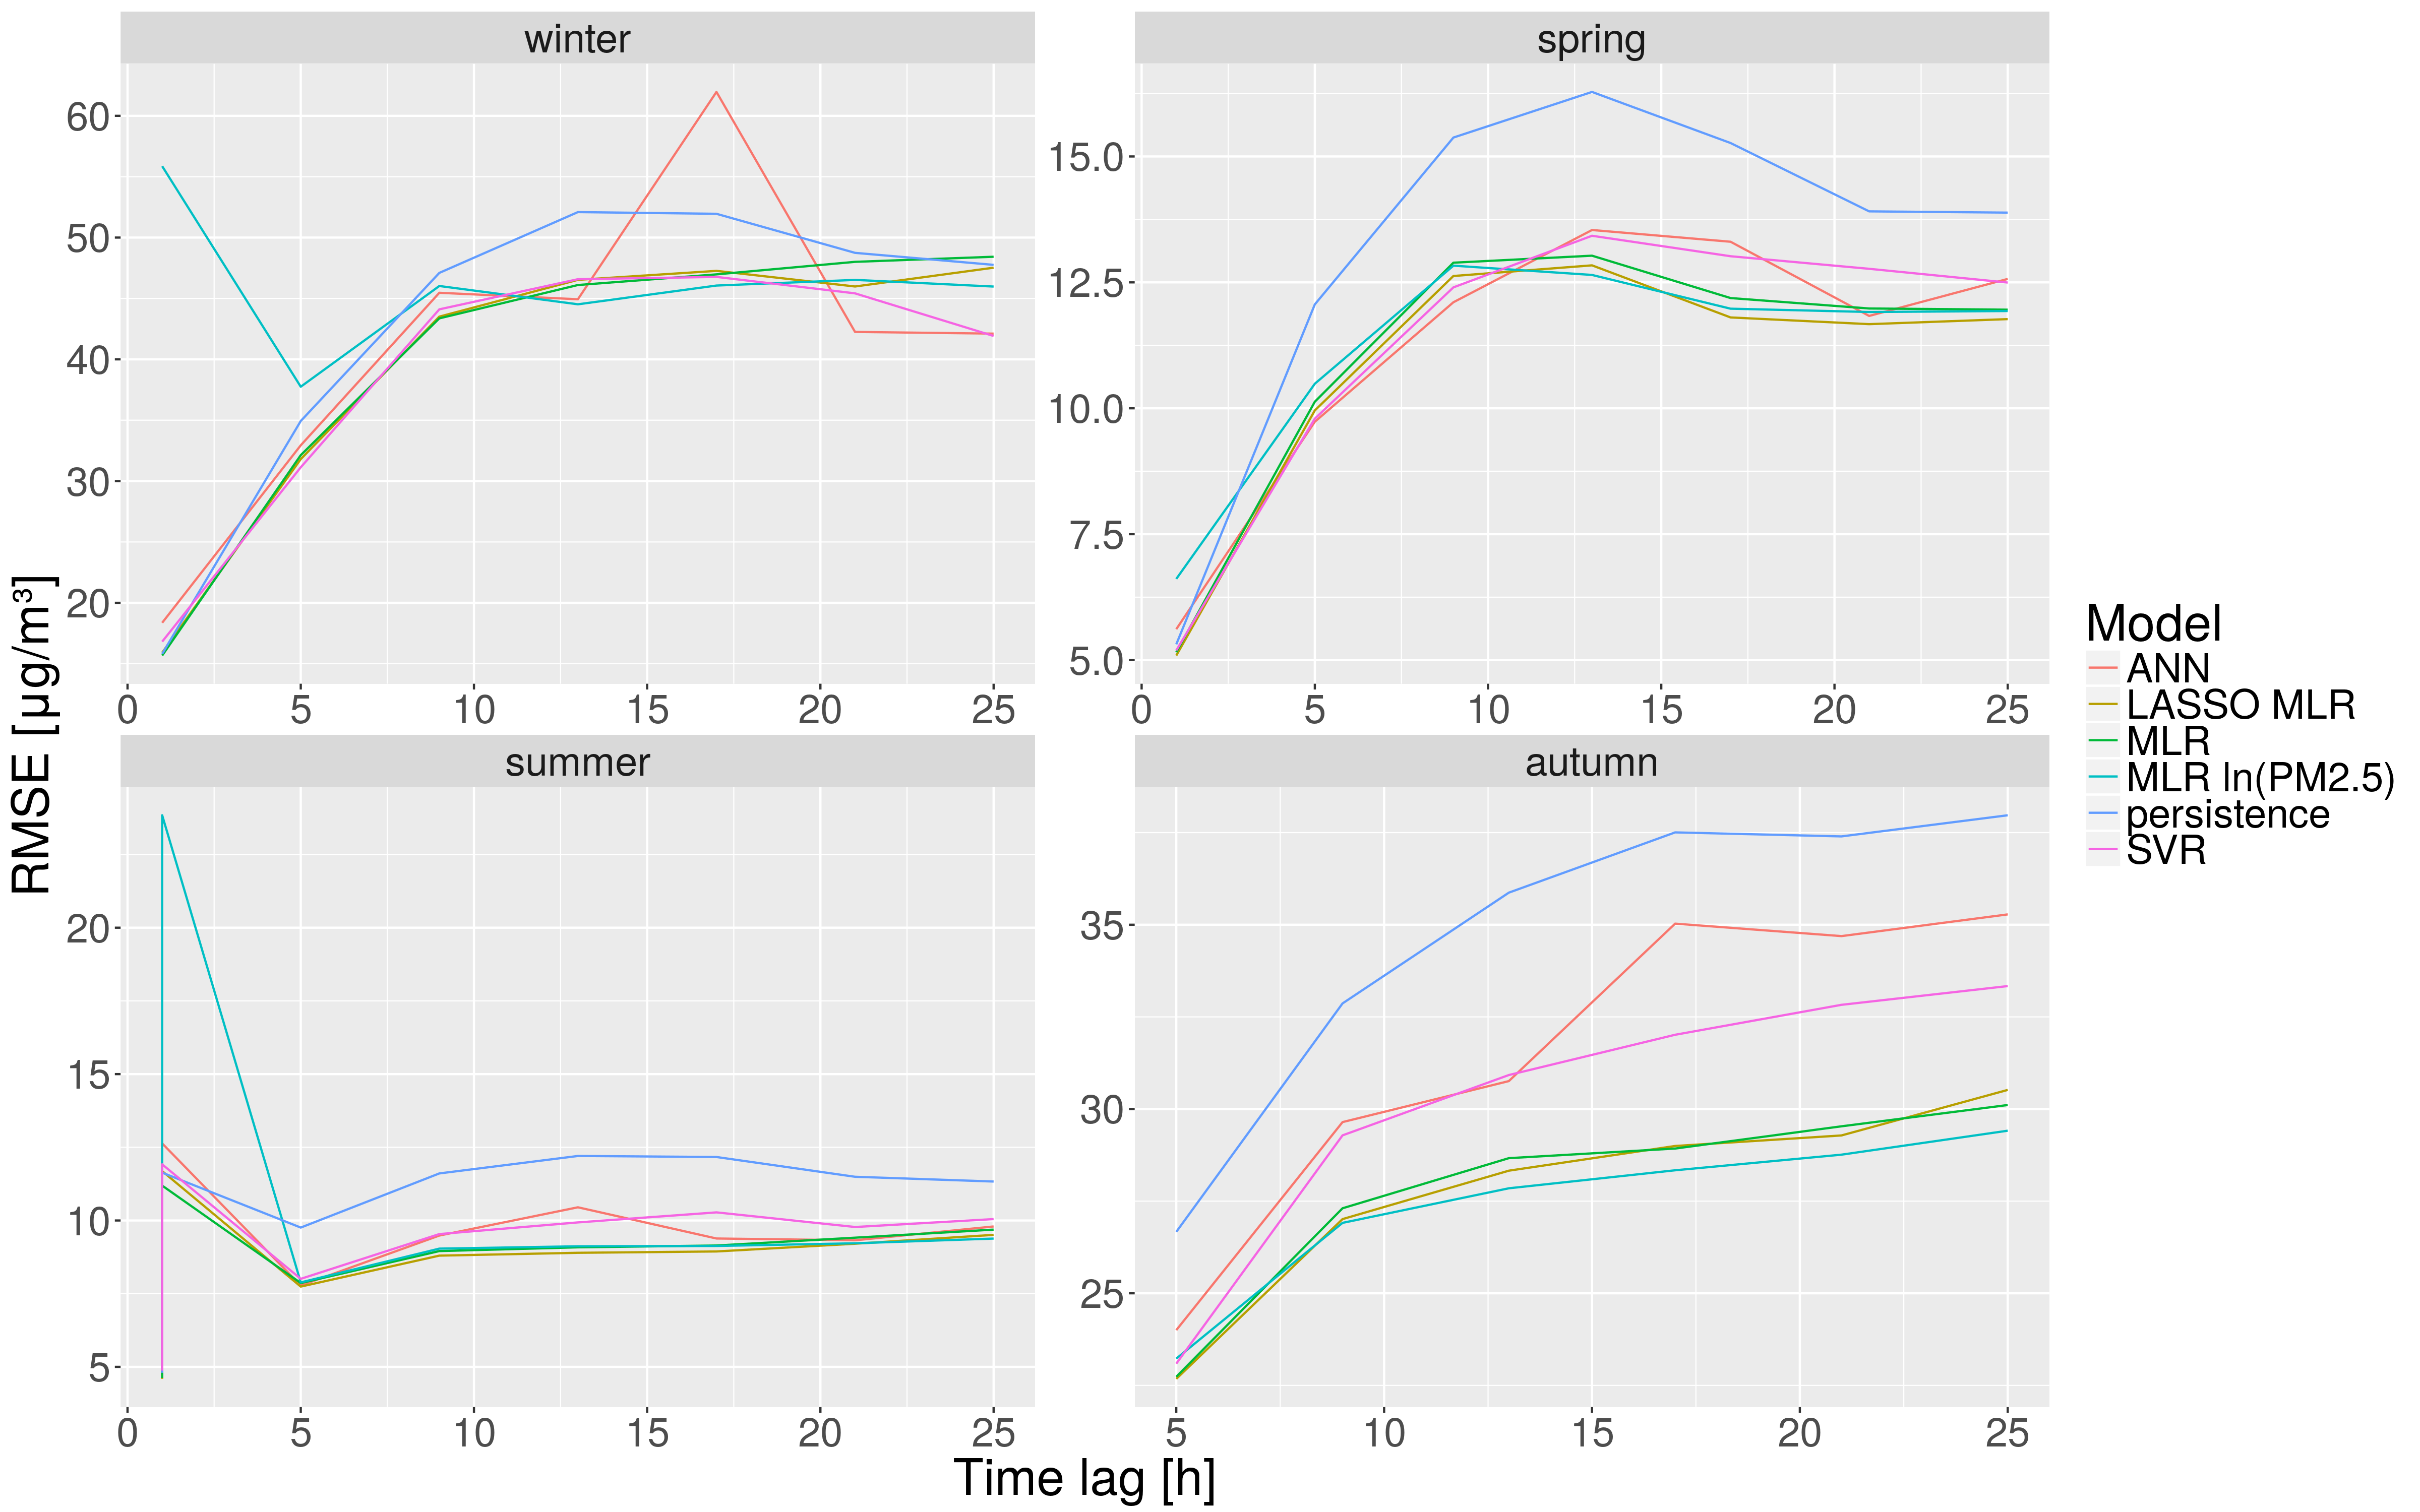
\includegraphics[width=0.9\linewidth]{figures/methodology/time-lag/rmse_time_lag.png}
  \caption{Root mean square errors for different time lags}
  \label{fig:methodology-time-lag}
\end{figure}

\section{Forecasting models}\label{sec:methodology-predictive-models}
This section provides a theoretical overview of the predictive models used in this study. 

\subsection{Multiple Linear Regression}\label{sec:models-regression}
Multiple linear regression is a method which assumes that the forecasted variable is dependent on a linear combination of explanatory variables (equation \ref{eq:models-regression}).
\begin{equation}\label{eq:models-regression}
    y_i = {\beta}_0 + \sum_{j = 1}^{p} {{\beta}_j x_{ij}} + {\epsilon}_i
\end{equation}
Meaning of the symbols used in the equation is as follows: $y_i$ is the $i^{th}$ value of the response variable, $x_ij$ is the $i^{th}$ value of the $j^{th}$ explanatory variable with ${\beta}_i$ being the corresponding weight, ${\beta}_0$ is the intercept which can be interpreted as the mean value of the response variable when all of the explanatory variables are equal to 0, $p$ is the number of dependent variables, ${epsilon}_i$ is the error factor expressing the difference between the actual and predicted values of the response variable. 
The goal of regression is to find such values of the parameters $\beta$ that the the sum of squared errors is minimised (equation \ref{eq:models-regression-sse}, symbol $\hat{y_i}$ is the $i^{th}$ actual value of the response variable).
\begin{equation}\label{eq:models-regression-sse}
    SSE = \sum_{i=1}^{n} {(y_i -  \hat{y_i})^2} = \sum_{i = 1}^{n} {{\epsilon}_i}^2
\end{equation}
In order to do so, it is convenient to rewrite equation \ref{eq:models-regression} to a matrix notation \ref{eq:models-regression-matrix}.
\begin{equation}\label{eq:models-regression-matrix}
    \begin{bmatrix}
        y_1 \\
        y_2 \\
        \vdots \\
        y_n
    \end{bmatrix}
    =
    \begin{bmatrix}
        1 & x_{1, 1} & x_{1, 2} & \hdots & x_{1, p} \\
        1 & x_{2, 1} & x_{2, 2} & \hdots & x_{2, p} \\
        \vdots   & \vdots   & \ddots & \vdots   \\
        1 & x_{n, 1} & x_{n, 2} & \hdots & x_{n, p} \\
    \end{bmatrix}
    \begin{bmatrix}
        {\beta}_0 \\
        {\beta}_1 \\
        {\beta}_2 \\
        \vdots \\
        {\beta}_p
    \end{bmatrix}
    +
    \begin{bmatrix}
        {\epsilon}_1 \\
        {\epsilon}_2 \\
        \vdots \\
        {\epsilon}_n
    \end{bmatrix}
\end{equation}
Now the sum of squared errors can be represented as \ref{eq:models-regression-sse-matrix}.
\begin{equation}\label{eq:models-regression-sse-matrix}
    SSE =
    \bm{\epsilon}^T \bm{\epsilon} = 
    \begin{bmatrix}
        {\epsilon}_1 & {\epsilon}_2 & \hdots & {\epsilon}_n
    \end{bmatrix}
    \begin{bmatrix}
        {\epsilon}_1 \\
        {\epsilon}_2 \\
        \vdots \\
        {\epsilon}_n
    \end{bmatrix}
    = \sum_{i = 1}^{n} {{\epsilon}_i}^2
\end{equation}
\begin{equation}
    \bm{\epsilon}^T \bm{\epsilon} = (\bm{y} - \bm{X}\bm{\beta})^T (\bm{y} - \bm{X}\bm{\beta})
\end{equation}
The optimisation problem can be expressed as:
\begin{equation}\label{eq:models-regression-minimum}
    \min_{\bm{\beta}} (\bm{\epsilon}^T \bm{\epsilon}) = \min_{\bm{\beta}} (\bm{y}^T \bm{y} - 2\bm{\beta}^T \bm{X}^T \bm{y} + \bm{\beta}^T \bm{X}^T \bm{X \beta})
\end{equation}
The minimum of the error function must meet the first-order condition (FOC) which states that the derivative of the error function with respect to the parameters vector $\beta$ must be equal to 0, which is expressed by equation \ref{eq:models-regression-derivative}. In the case of the last component of the right-hand side expression of equation \ref{eq:models-regression-minimum} the product rule was used.
\begin{equation}\label{eq:models-regression-derivative}
    \frac{\partial{(\bm{\epsilon}^T \bm{\epsilon})}}{\partial{\beta}} = 0 - 2 \bm{X}^T \bm{y} + \bm{X}^T\bm{X}\bm{\beta} + \bm{\beta}^T\bm{X}^T\bm{X} = 0
\end{equation}
Since the values of the expressions
\begin{align}
 \bm{X}^T\bm{X}\bm{\beta} \\
 \bm{\beta}^T\bm{X}^T\bm{X}
\end{align}
are scalars and because of the fact that
\begin{equation}
 \bm{X}^T\bm{X}\bm{\beta} = (\bm{\beta}^T\bm{X}^T\bm{X})^T
\end{equation}
equation \ref{eq:models-regression-derivative} might be rewritten as:
\begin{equation}
    \frac{\partial{(\bm{\epsilon}^T \bm{\epsilon})}}{\partial{\beta}} = -2 \bm{X}^T \bm{y} + 2\bm{X}^T\bm{X}\bm{\beta} = 0
\end{equation}
Note that the transpose of a scalar is the same scalar. Now we can express the coefficient vector $\beta$, using the matrix $\bm{X}$ and the vector $\bm{y}$ (equations \ref{eq:model-regression-coefficients} and \ref{eq:model-regression-coefficients-final}), provided that the matrix $\bm{X}^T\bm{X}$ is invertible.

\begin{equation}\label{eq:model-regression-coefficients}
  \bm{X}^T\bm{X}\bm{\beta} = \bm{X}^T \bm{y}
\end{equation}

\begin{equation}\label{eq:model-regression-coefficients-final}
  \bm{\beta} = (\bm{X}^T\bm{X})^{-1} (\bm{X}^T \bm{y})
\end{equation}
Additionally, in order to satisfy the second order condition for a minimum, the matrix $\bm{X}^T\bm{X}$ must be positive definite (equation \ref{eq:model-regression-soc}), which is true if the matrix is non-singular (\cite{LAI2008}).

\begin{equation}\label{eq:model-regression-soc}
    \forall {\bm{v} \in \R^{p}, \bm{v} \neq \bm{0}}: \: \bm{v}(\bm{X}^T\bm{X})\bm{v}^T > 0
\end{equation}
It is worth noting that applicability of multiple regression models is limited by several assumptions that must be met by the data set, e.g.: 
\begin{itemize}
    \item linear relationship between the response variable and predictors,
    \item independence of the response variable values,
    \item normal distribution of the errors with mean equal to zero,
    \item lack of perfect collinearity between the predictors,
    \item lack of correlation between the predictors and error terms,
    \item constant variance of errors all predictor combinations     (\textit{homoscedascicity}),
    \item lack of autocorrelation between the error terms.
\end{itemize}
A more detailed description of the mentioned assumptions can be found in \cite{HOFFMAN2008}.

\subsection*{LASSO regression}
Least Absolute Shrinkage and Selection Operator Regression (LASSO) is a variant of multiple linear regression which includes a variable selection mechanism. It may be beneficial to get rid of unnecessary variables in order to simplify the final model, making it work faster and prevent it from overfitting to the training data. Variables are removed from the model by setting their coefficients ($\bm{\beta}$) in the regression equation to zero. Such an effect is achieved by modifying the formulation of the optimisation problem by adding a term dependent on the coefficients (equation \ref{eq:models-lasso-minimum}). The parameter $\lambda \geq 0$ expresses the strength of the penalty for large coefficients \cite{FONTI2017}.

\begin{equation}\label{eq:models-lasso-minimum}
    \min_{\bm{\beta}} (\bm{\epsilon}^T \bm{\epsilon}) = \min_{\bm{\beta}} ((\bm{y} - \bm{X}\bm{\beta})^T (\bm{y} - \bm{X}\bm{\beta}) + \lambda \sum_{j = 1}^{p} |{\beta}_j|)
\end{equation}

\subsection{Support Vector Regression}
Another method of fitting a linear function to a set of observations is the Support Vector Regression (SVR). Its goal is to find a function $f(x)$ that approximates the available data points in such a way that in all cases the absolute difference between the actual value of the response variable and the value of the fitted function is not higher than $\epsilon$ (an input parameter). An additional condition taken into consideration states that the magnitude of input weights should be as small as possible. The optimisation problem can be formulated as shown in equation \ref{eq:models-svr-optimisation}.
\begin{equation}\label{eq:models-svr-optimisation}
\begin{gathered}
    \text{minimize}\, \frac{1}{2} {\lVert {w} \rVert}^2 \\
    \text{subject to}
    \begin{cases}
        y_i - (\langle \bm{w}, \bm{x_i} \rangle + w_0, & \leq \epsilon \\
        (\langle \bm{w}, \bm{x_i} \rangle + w_0) - y_i, & \leq \epsilon
    \end{cases}
\end{gathered}
\end{equation}
Symbols used in equation \ref{eq:models-svr-optimisation} have the following meaning: $y_i$ is the $i^{th}$ actual value of the response variable, $\bm{w}$ is the vector of input weights, $\bm{x_i}$ is the $i^{th}$ vector of predictor values, $\langle \cdot, \cdot \rangle$ is the dot product, $\epsilon$ is the assumed tolerance margin. 
In some cases the function $f(x)$ may not exist. Because of that additional variables $\xi, {\xi}^*$ representing the exceedance of the tolerance limit are introduced into the problem formulation (equation \ref{eq:models-svr-optimisation-soft}).

\begin{equation}\label{eq:models-svr-optimisation-soft}
\begin{gathered}
    \text{minimize}\, \frac{1}{2} {\lVert {w} \rVert}^2 + C\sum_{i = 1}^{n} ({\xi}_i + {{\xi}_i}^*) \\
    \text{subject to}
    \begin{cases}
        y_i - (\langle \bm{w}, \bm{x_i} \rangle + w_0, & \leq \epsilon + {\xi}_i \\
        (\langle \bm{w}, \bm{x_i} \rangle + w_0) - y_i, & \leq \epsilon + {{\xi}_i}^* \\
        {\xi}_i + {{\xi}_i}^* \geq 0
    \end{cases}
\end{gathered}
\end{equation}
The $C$ coefficient controls the strength of the penalty corresponding to the data points laying outside the tolerance margin. The problem stated in equation \ref{eq:models-svr-optimisation-soft} is an example of a quadratic programming problem and can be solved using the Lagrange multipliers method. For a more detailed description of the procedure refer to \cite{SMOLA2003}.
\\\\
It is worth noting that an SVR model can be adapted to fitting nonlinear functions by transforming the data points (actually their dot product, which is required by the optimisation procedure), using a kernel function and performing optimisation in the new feature space. A kernel function takes the form of a dot product shown in equation \ref{eq:models-svr-kernel}. In this study a radial basis function kernel defined in equation \ref{eq:models-svr-kernel-rbf} was used.

\begin{equation}\label{eq:models-svr-kernel}
K(\bm{x}, \bm{x'}) = \langle \Phi(\bm{x}), \Phi(\bm{x'}) \rangle
\end{equation}

\begin{equation}\label{eq:models-svr-kernel-rbf}
K(\bm{x}, \bm{x'}) = e^{-\gamma {\lVert \bm{x} - \bm{x'} \rVert}^2}
\end{equation}

\subsection{Neural networks}
An artificial neural network (ANN) is a network comprised of connected processing units called neurons. A neuron is capable of calculating a linear combination of its inputs and an additional parameter called bias which has a similar role to the intercept in linear regression. The output of a neuron is passed as an argument to an activation function for example a sigmoidal function \ref{eq:models-neural-sigmoid}.

\begin{equation} \label{eq:models-neural-sigmoid}
g(x) = \frac{1}{1 + e^{-x}}
\end{equation}
Thus, the value calculated by the $j^{th}$ neuron can be expressed as in equation \ref{eq:models-neural-neuron}.

\begin{equation} \label{eq:models-neural-neuron}
y_j = g(\sum_{i} w_i x_i + b_j)
\end{equation}
where $w_i$ is the weight of the $i^{th}$ input value $x_i$, $g$ is the activation function and $b_j$ is the bias corresponding to the neuron. Expression \ref{eq:models-neural-neuron} can be visualised as shown in figure \ref{fig:models-neuron}.

\begin{figure}[H]
\centering
\includegraphics[scale=1.00]{figures/models/neuron.png}
\caption{An artificial neuron}
\label{fig:models-neuron}
\end{figure}
%
As pointed by \cite{BISHOP1995}, a single neuron can be used as a binary classifier in the case of two linearly separable classes. Combining $n$ neurons in a single-layer network allows to classify members of $n$ classes separable with a hyperplane. Two-layered networks are capable of recognising members of a class represented by a convex region. Networks with three layers or more can represent arbitrary decision regions with an arbitrary precision.
It's worth noting that the term n-layered network refers in this case to the number of layers of hidden (other than input and output) neurons.

\subsection*{Feedforward networks}
One of the common ways of designing ANNs is to make neurons from layer $n$ have inputs only from layer $n-1$ and outputs passed to layer $n+1$. Neurons in the layer $n$ are fully connected with neurons in the layer $n+1$. Networks that are organised in such a fashion are called feedforward neural networks. One of the benefits of such architecture is the ease of analysis and designing learning algorithms. 
An example of a feedforward network is shown in figure \ref{fig:models-feedforward-network}. For the sake of clarity it is assumed that evaluation of the activation function is integrated into the processing units. The solid black circles represent bias inputs.

\begin{figure}[H]
\centering
\includegraphics[scale=0.6]{figures/models/feedforward-network.png}
\caption{A two-layered feedforward network}
\label{fig:models-feedforward-network}
\end{figure}

\subsection*{Network training}\label{ssec:network-training}
The goal of network training is to optimise its classification accuracy by gradually updating the input weights of neurons. The following description is based on \cite{HAN2005}.
Before the training starts input data is divided into two subsets: training and test. Weights of the neuron inputs are set randomly.
The next phase is called forward propagation. Samples from the training set (in the form of floating-point valued vectors) are passed as inputs to the network. The output values of the neurons in the first hidden layer are computed and passed to the next layer, etc. The process is repeated until the network outputs are calculated.
Now it is possible to verify network's accuracy by computing the value of a chosen error function, for example a standard sum of squares function
\begin{equation}
SSE = \frac{1}{2}\sum_{i=1}^{n}(y_i - t_i)^2
\end{equation}
where $n$ is the number of outputs and $t_i$ refers to the actual value of the $i^{th}$ output (it is known for the training samples).
In order to adjust the input weights so that the prediction error is decreased it is necessary to perform a step called error back-propagation. It is a process of computing the error term corresponding to a specific neuron based on the errors of the neurons from the next layer. Back-propagation starts with calculating errors for each of the outputs, which can be formulated in the form of equations \ref{eq:models-neural-error} and \ref{eq:models-neural-neuron-output}

\begin{equation}\label{eq:models-neural-error}
Err_j = g'(a_j) (t_j - y_j)
\end{equation}
\begin{equation}\label{eq:models-neural-neuron-output}
a_j=\sum_{i} w_{ij} z_i
\end{equation}
where $g'$ is the derivative of the activation function, $t_j$ is the actual value of the $j^{th}$ output, $z_i$ is the $i^{th}$ input of the neuron and $w_{ij}$ is its weight. Fortunately, for the sigmoid function derivative $g'(a_j)$ might be presented as equation \ref{eq:models-neural-sigmoid-derivative}, and thus easily computed. Derivation of a generalised expression equivalent to \ref{eq:models-neural-sigmoid-derivative} can be found in \cite{BISHOP1995}.

\begin{equation} \label{eq:models-neural-sigmoid-derivative}
g'(a_j) = y_j (1 - y_j)
\end{equation}
Having found the value of $Err_j$ for the output neurons, it is possible to calculate errors for the last but one layer. The applicable expression takes the form of equation \ref{eq:models-neural-output-error}.

\begin{equation}\label{eq:models-neural-output-error}
Err_j = y_j(1-y_j) \sum_{k} Err_k w_{jk}
\end{equation}
Component $Err_k$ is the error of the k-th neuron in the output layer connected to the neuron $j$. Each time the error value is computed, it is used to update the weights in the gradient descent algorithm as presented in equations \ref{eq:models-neural-weight-change} and \ref{eq:models-neural-new-weight}.

\begin{equation}\label{eq:models-neural-weight-change}
\Delta w_{ij} = \mu Err_j y_i
\end{equation}
\begin{equation}\label{eq:models-neural-new-weight}
w_{ij} = w_{ij} - \Delta w_{ij}
\end{equation}
The $\mu$ factor expresses the learning rate. It has been introduced in order to prevent the algorithm from getting stuck in a local optimum
\\
The learning procedure can be stopped after a specific condition has been reached, for example:
\begin{itemize}
	\item the changes of all weights in the last iteration were smaller than a specified threshold; 
	\item the target number of iterations has been reached;
	\item the requirement of maximum percentage of misclassification has been met.
\end{itemize}

\section{Testing procedure} \label{sec:methodology-testing-procedure}
Accuracy of prediction of each model investigated in this study was verified using the cross validation technique. The data set was split into two groups: observations from the period 2014 - 2016 were used only as training samples, while the test set was comprised of measurements taken in 2017. Each model was tested separately for each of four astronomical seasons defined as shown in table \ref{methodology:seasons}.
\begin{table}[H]
\centering
\caption{Beginning and end dates of astronomical seasons in Poland}
\label{methodology:seasons}
\begin{tabular}{lll}
\toprule
Season & Start date & End date \\ \midrule
Winter & December 21 & March 21 \\
Spring & March 21 & June 22 \\
Summer & June 22 & September 23 \\
Autumn & September 23 & December 21 \\ \bottomrule
\end{tabular}
\end{table}
\noindent Each test set was additionally divided into three time windows containing measurements from 28 days. After saving results from all models for the current window, it was included in the training set and the models were trained again. The goal of this approach is to test the accuracy of predictions made for previously unavailable input data. Figure \ref{fig:methodology-time-windows} contains a visualisation of the process.

\begin{figure}[H]
\centering
      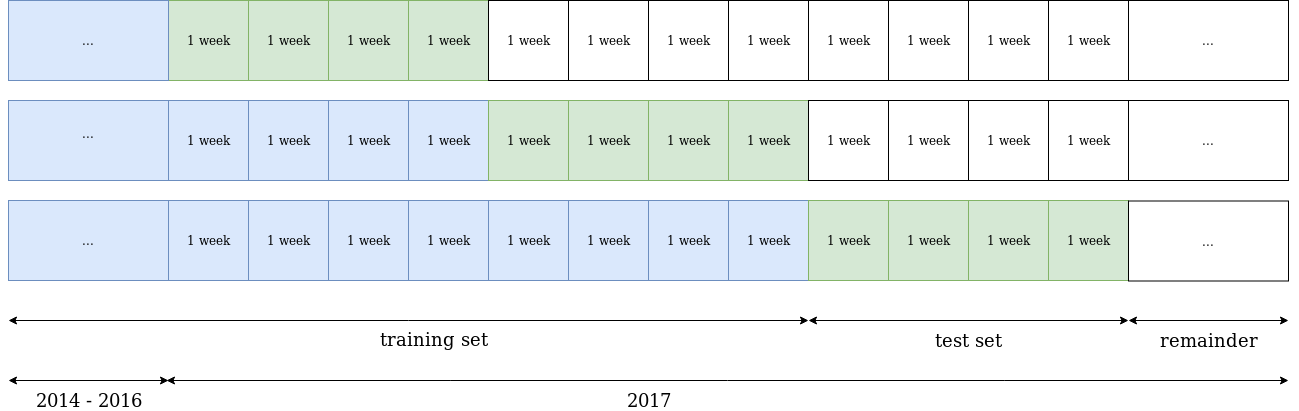
\includegraphics[width=\textwidth]{figures/methodology/time_windows.png}
      \caption{Implementation of sliding time windows used in the study}
      \label{fig:methodology-time-windows}
\end{figure}
\noindent Two variants of the training procedure were used in the study. The first one consisted in training models only on the data registered during the same season as the one that the test observations come from. The second strategy assumed that the training set should be made of all available measurements taken before the start of the test time window. Figures \ref{fig:methodology-training-same-season}  and \ref{fig:methodology-training-all-data} depict how the data are split according to each method. The training set is marked as blue, while the test set - as red.
\begin{figure}[H]
\centering
  \centering
  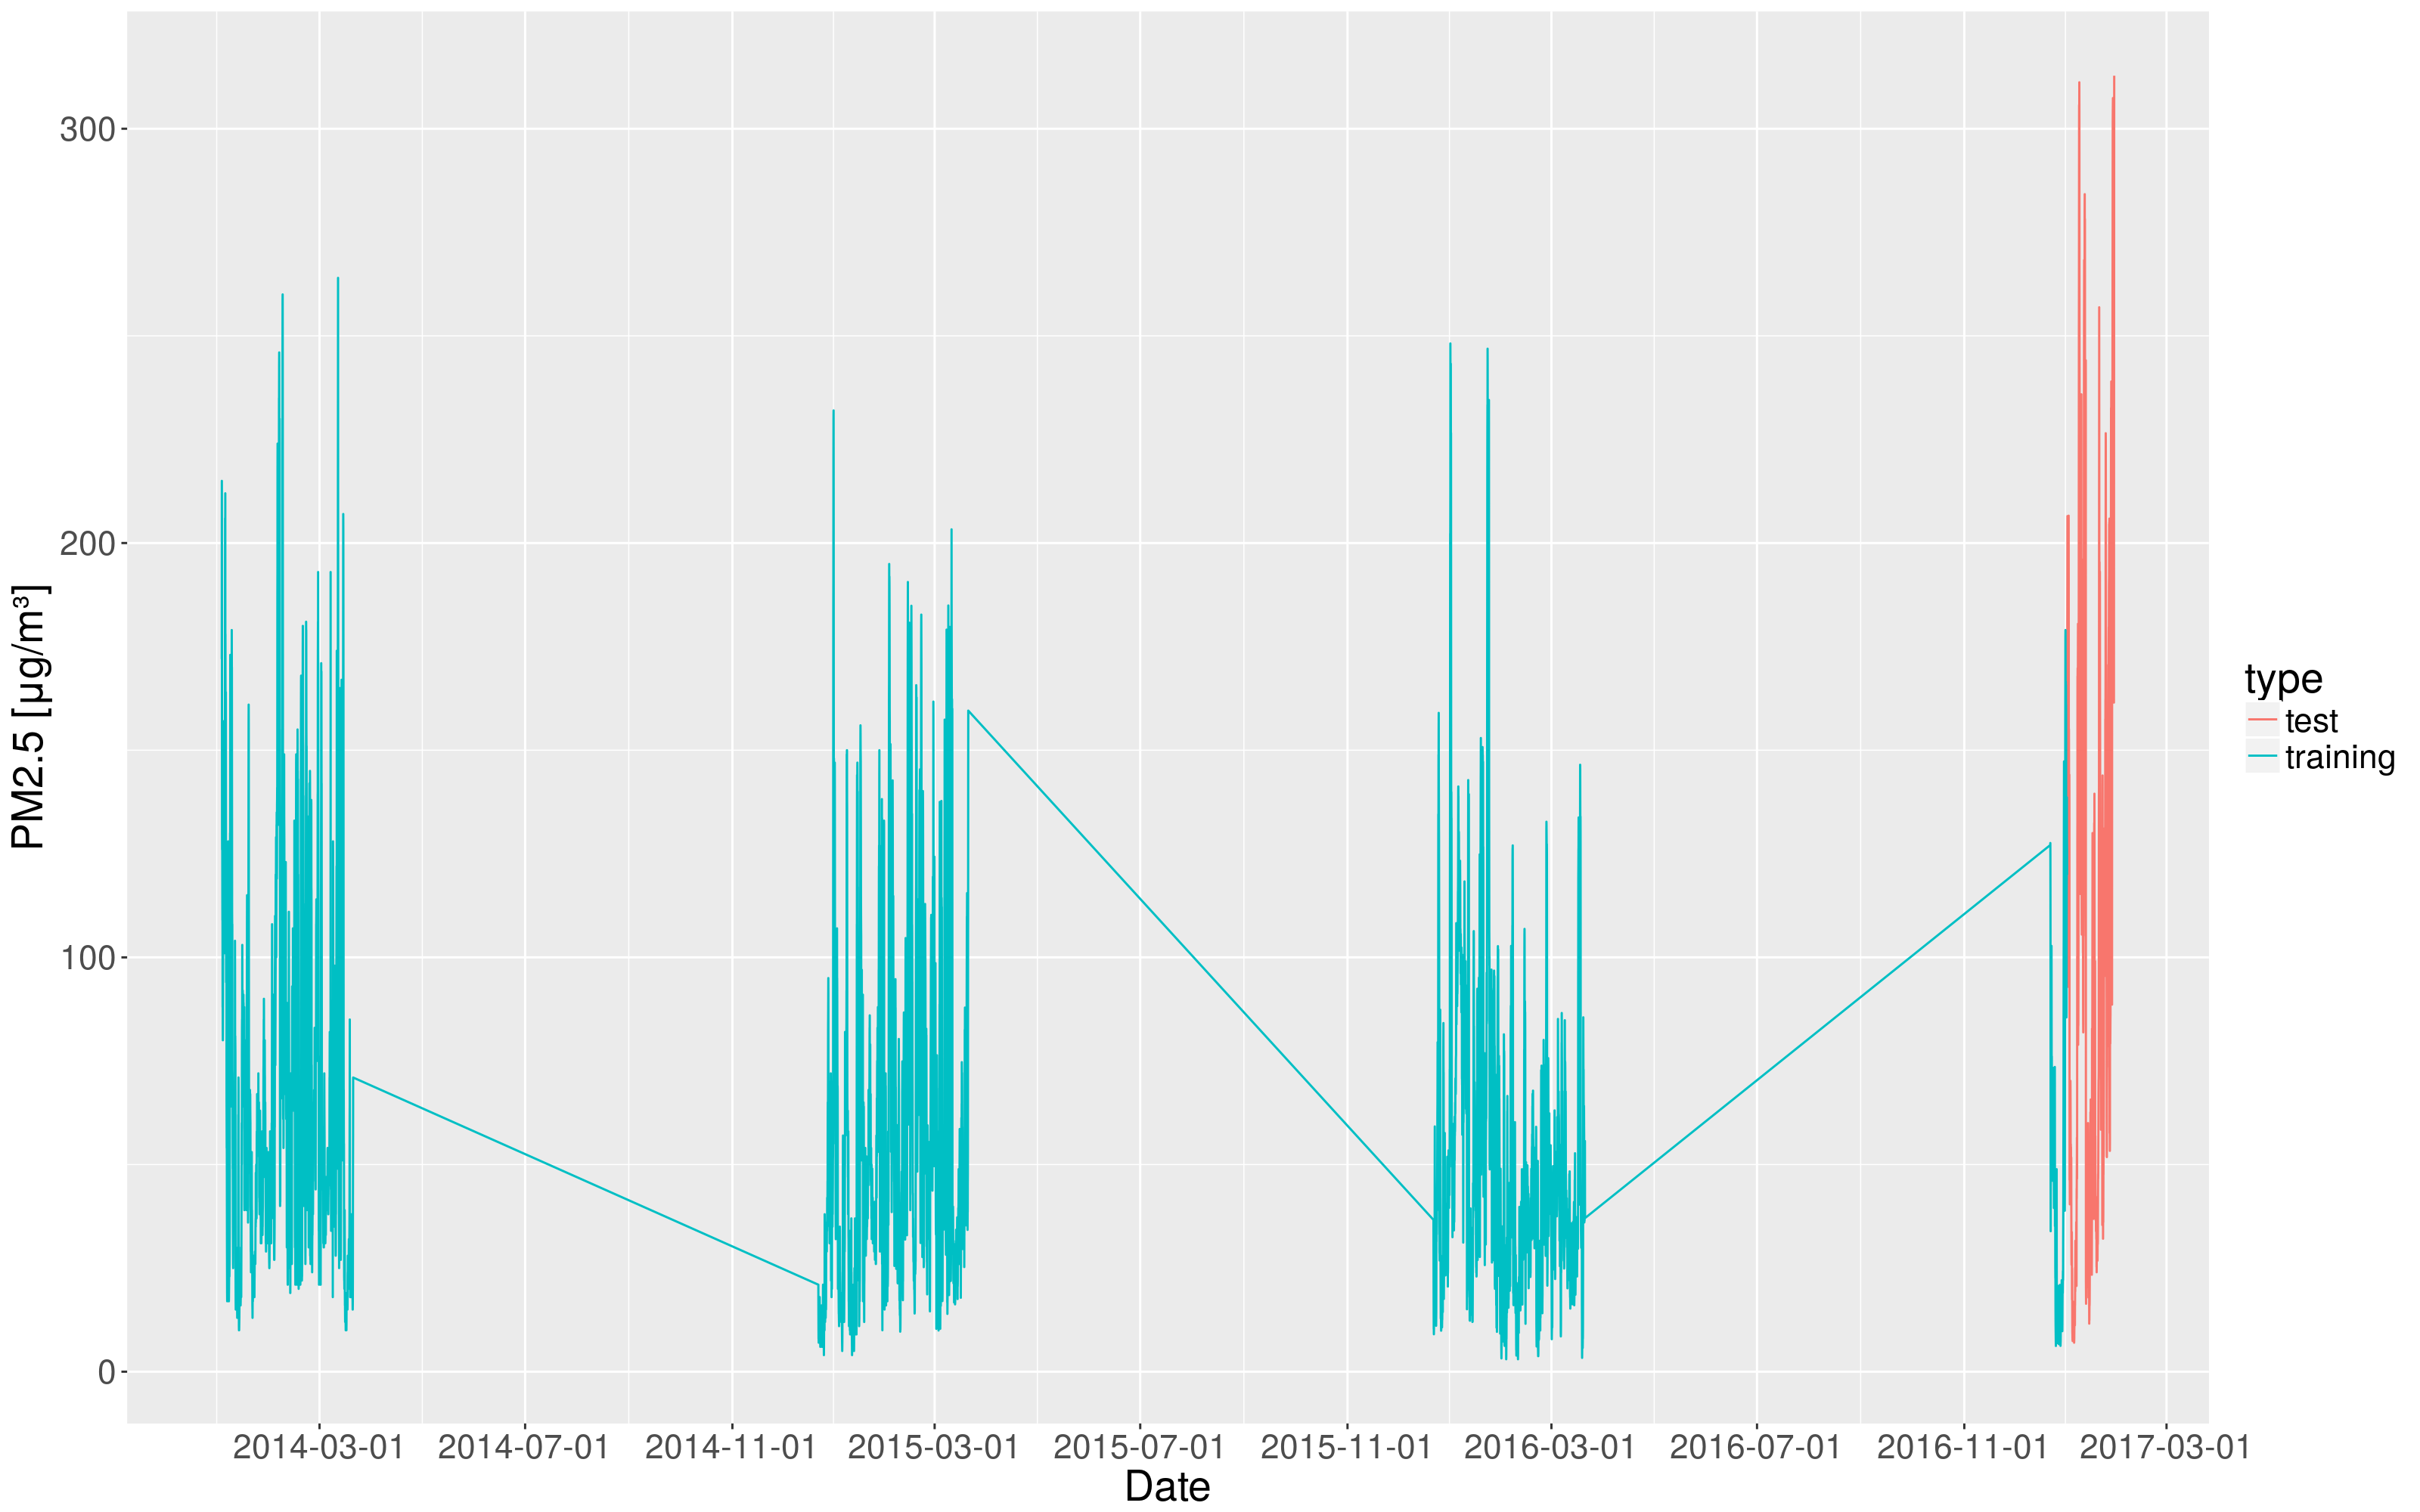
\includegraphics[width=0.95\linewidth]{figures/methodology/split/same_season_split_1.png}
  \caption{Training strategy - same season (winter)}
  \label{fig:methodology-training-same-season}
\end{figure}
\begin{figure}[H]
\centering
  \centering
  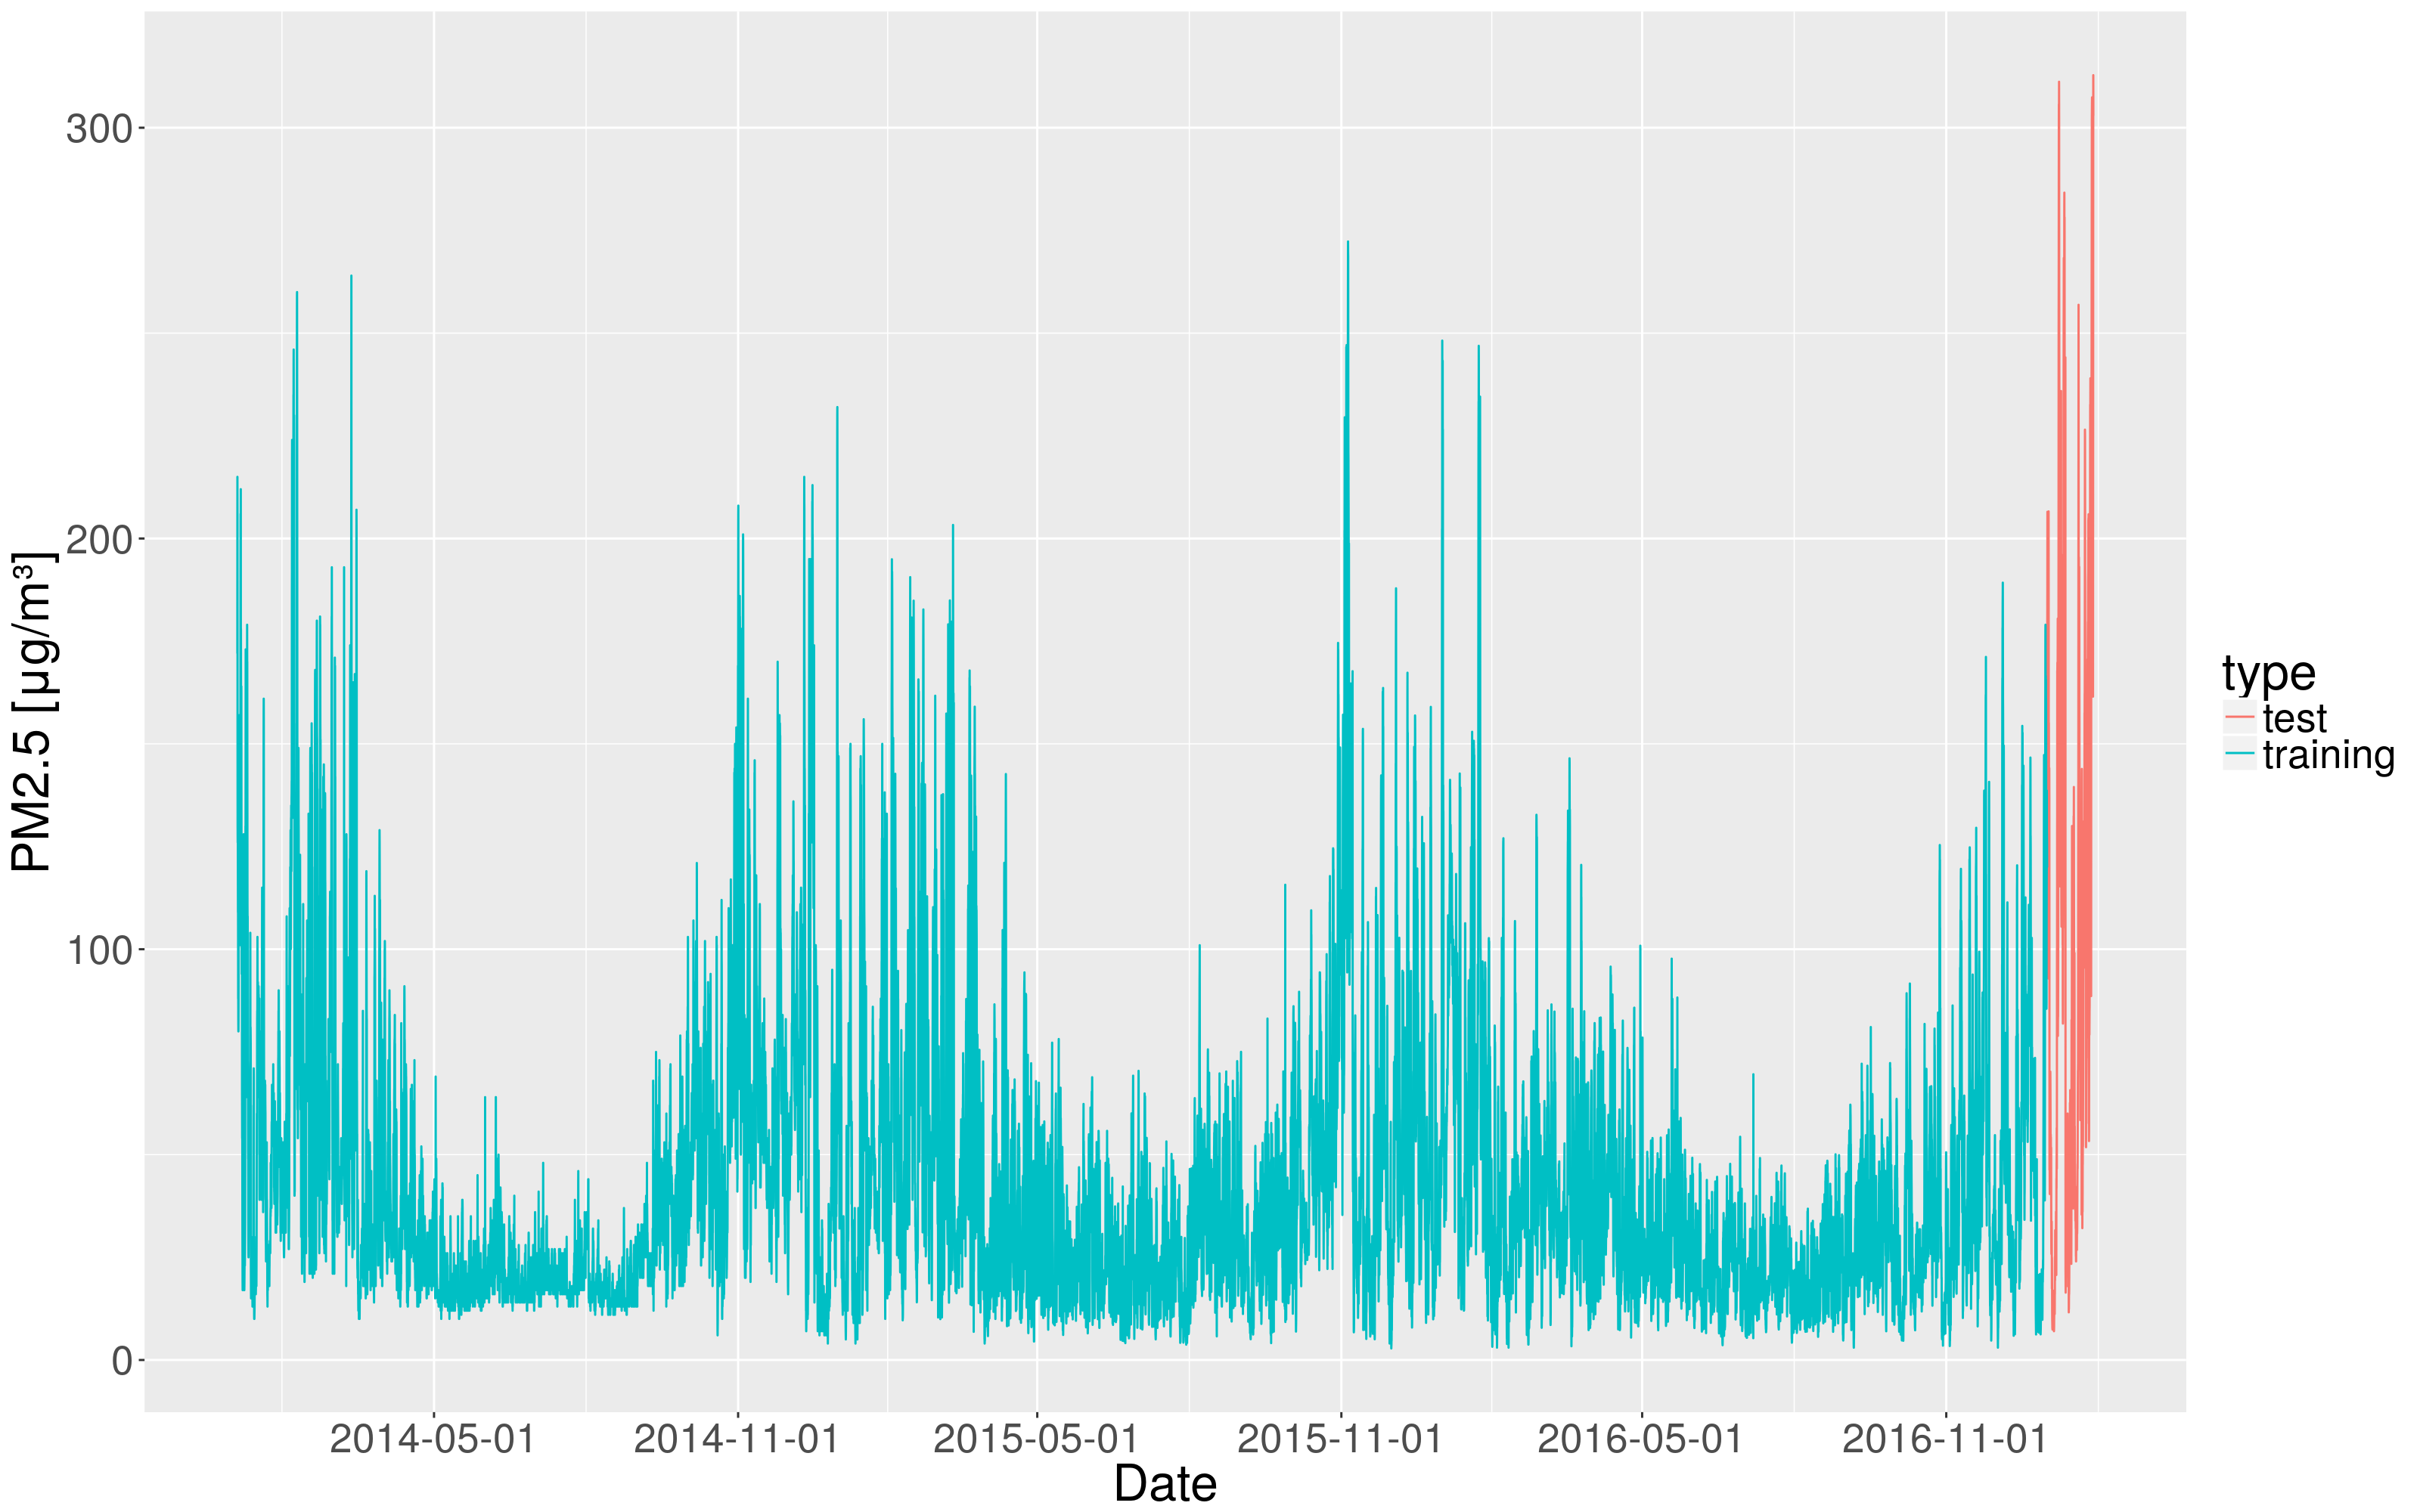
\includegraphics[width=0.95\linewidth]{figures/methodology/split/continuous_split_1.png}
  \caption{Training strategy - all historical data (winter)}
  \label{fig:methodology-training-all-data}
\end{figure}

\noindent Some of the used models - all variants of linear regression - are straightforward when it comes to usage - they require only passing inputs, while the remaining ones need an additional step of hyperparameter tuning. Because of its time consuming nature, it was conducted only for the Krasińskiego station and the best found configurations were later applied to the remaining stations. The exact procedure varied for different model types.
\\\\
\noindent In the case of support vector regression the best configuration of three parameters was0 searched for: gamma, epsilon and cost (their meaning is described in the documentation of the \textit{e1071} package for R \cite{E1071SVM2017}). Since it is not possible to test all of them, a range of allowed values was defined for each parameter, which can be found in table \ref{tab:methodology-svr-params}. The idea of using powers of 2 is based on \cite{HSU2010}. The tested models were trained for 50 unique, randomly picked combinations of the listed values. Other options were left unchanged, for example each SVR model used a radial basis function as kernel.
\begin{table}[ht]
\centering
\caption{Values of SVR parameters considered in the study}
\label{tab:methodology-svr-params}
\begin{tabular}{ll}
\toprule
Parameter & Values \\ \midrule
cost & $2^{-2}$, $2^{0}$, $2^{2}$, $2^{4}$, $2^{6}$, $2^{8}$, $2^{10}$ \\
epsilon & $2^{-5}$, $2^{-3}$, $2^{-1}$, $2^{1}$ \\
gamma & $2^{-12}$, $2^{-10}$, $2^{-8}$, $2^{-6}$, $2^{-4}$ \\ \bottomrule
\end{tabular}
\end{table}
When it comes to artificial neural networks, the following parameters were investigated: number of hidden layers (at most 2), number of neurons in hidden layers and threshold value for the derivatives of the error function (stopping condition). In each case the same type of the network (a multilayer perceptron), maximum number of epochs (1 mln), activation function (logistic/sigmoid) and training algorithm (resilient backpropagation with weight backtracking) were used. The process of optimisation was divided into three steps. At the beginning, a few manually picked architectures were tested with a fixed threshold value. The networks consisted of hidden layers with the following numbers of neurons: 5, 10, 15, 3-3, 5-3, 5-5, 7-5, 10-7. It is worth noting that, because of the random initialisation of the input weights, each network prepared for the specific test window was actually trained three times and the final forecast was averaged. At the next step architectures with the number of neurons differing from the best one found in the previous stage at most by 1 for each of the hidden layers were investigated. For example if the best network had two layers both with 5 neurons (5, 5) the considered networks would have 4, 5 or 6 neurons in each of the hidden layers. The final step consisted in testing the best found architecture with a few threshold values ranging from 0.7 to 0.1 (0.3 when using all available data). Each configuration was trained five times in order to make sure the results are fairly consistent.


\chapter{Data set}\label{chap:dataset}
This chapter provides a description of the gathered data set. It discusses the data sources, included variables, their statistics and relationships between them.

\section{Air quality data}\label{sec:air-quality-data}

The data concerning the air quality were obtained from the General Inspectorate of Environmental Protection (further referred as GIOŚ from Polish \textit{Główny Inspektorat Ochrony Środowiska}). Observations were registered by three monitoring stations nearby the following streets: Krasińskiego, Bujaka, Bulwarowa. The measurements come from the period between January 1, 2014 and December 31, 2017. Locations of the stations were presented in table \ref{tab:dataset-stations-location} and in figure \ref{fig:dataset-stations-location}, both of which are based on the information available at the official website of the Inspectorate \cite{GIOSLOCATION2018}. Stations used in this study are marked with red circles. 

\begin{table}[ht]
\centering
\caption{Location of the air quality stations}
\label{tab:dataset-stations-location}
\begin{tabular}{lll}
\toprule
Station           & Latitude ($\degree$ North) & Longitude ($\degree$ East) \\ \midrule
GIOŚ Bujaka       & 50.010575                  & 19.949189                  \\
GIOŚ Bulwarowa    & 50.069308                  & 20.053492                  \\
GIOŚ Krasińskiego & 50.057678                  & 19.926189                  \\ \bottomrule
\end{tabular}
\end{table}

\begin{figure}[ht]
\centering
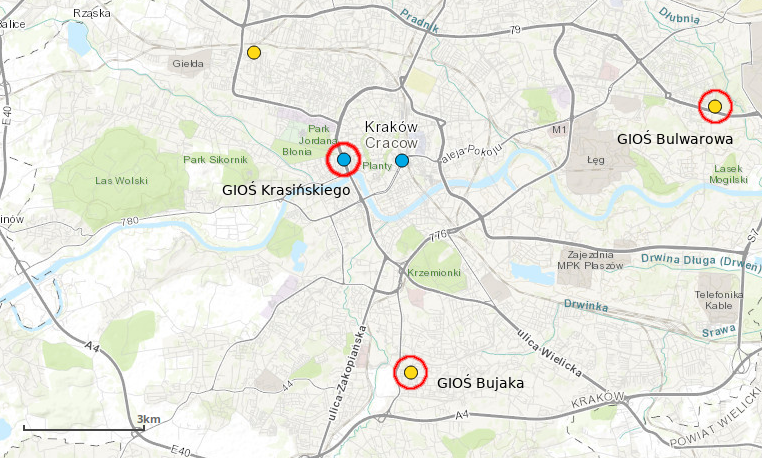
\includegraphics[scale=0.5]{figures/dataset/gios_stations.png}
\caption{Location of the air quality stations}
\label{fig:dataset-stations-location}
\end{figure}

\section{Weather factors}\label{sec:weather-data}
Air quality monitoring stations used in this study are not equipped with sensors measuring weather factors. Because of that it was decided to combine the PM2.5 measurements with meteorological data obtained from other sources: a weather station (specifically Vaisala WXT520) operated by the Faculty of Physics and Computer Science at the AGH University, sensors belonging to Airly (a local air quality monitoring company) and the Weather Underground service. The following weather variables were used in this study:
\begin{enumerate}
    \item atmospheric pressure,
    \item humidity,
    \item precipitation rate,
    \item total precipitation during the given day,
    \item temperature,
    \item wind speed,
    \item wind direction - divided into two components - North - South and East - West according to formulas \ref{eq:methodology-wind-dir-ns} and \ref{eq:methodology-wind-dir-ew}, where ${dir}_{deg}$ means wind direction expressed in degrees; directions correspond to the following angles: North - 0 $\degree$, East - 90 $\degree$, South - 180 $\degree$, West - 270 $\degree$; a visual interpretation of the variables can be seen in figure \ref{fig:dataset-wind-direction-components}.
\end{enumerate}

\begin{equation} \label{eq:methodology-wind-dir-ns}
{dir}_{North-South}({dir}_{deg}) =  sin({dir}_{deg}\frac{2 \pi}{360})
\end{equation}

\begin{equation} \label{eq:methodology-wind-dir-ew}
{dir}_{East-West}({dir}_{deg}) =  cos({dir}_{deg}\frac{2 \pi}{360})
\end{equation}
\\
\begin{figure}[htp]
    \centering
    
\includegraphics[scale=1]{figures/dataset/wind_direction.png}
    \caption{Wind direction components - North - South and East - West}
    \label{fig:dataset-wind-direction-components}
\end{figure}\\
Weather variables were combined with the PM2.5 concentrations based on the time of measurement and the geographical coordinates of the stations. The distances between stations were approximated by the formula \ref{eq:dataset-lat-lon-distance} based on the Spherical Law of Cosines, where $\phi$ symbolises the latitude and $\lambda$ is the longitude.

\begin{equation} \label{eq:dataset-lat-lon-distance}
dist(\phi_1, \lambda_1, \phi_2, \lambda_2) \approx acos(sin(\phi_1) sin(\phi_2) + cos(\phi_1)cos(\phi_2)cos(\lambda_2 - \lambda_1))
\end{equation}

\section{Additional variables}\label{sec:additional-variables}
The original data set was extended with a few auxiliary temporal variables intended to represent different types of seasonality, namely:
\begin{enumerate}
    \item hour of the day,
    \item period of the day - it is assumed that a 24-hour period consists of 4 parts: morning (6 a.m. - 12 p.m.), afternoon (12 p.m. - 6 p.m.), evening (6 p.m. - 12 a.m.), night (12 a.m. - 6 a.m.);
    \item day of the week,
    \item a flag indicating, whether the measurement was taken during a weekday or a weekend\,/\,a\,holiday (however, the movable holidays were not taken into consideration),
    \item month,
    \item day of the year,
    \item season - a numeric value in the range 1 - 4, where 1 represents winter, 2 - spring, 3 - summer, 4 - autumn,
    \item a flag indicating, if the measurement was taken during the heating season, which is assumed to start in September and end at the beginning of April,
    \item year.
\end{enumerate}
In the case of variables that express a fraction of a larger whole (e.g. day of the year = $\frac{day\  count}{365}$) their values were calculated as cosines of those fractions scaled and shifted in such a way, that the beginning and end of the period correspond with 0 while its centre to 1 (see equation \ref{eq:methodology-part-of-period}). Figure \ref{fig:dataset-cosine-transformation} shows the relationship between the day of the year and the value assigned to it (plots for other such variables are similar).
\\
For some variables (PM2.5 concentrations, relative humidity, precipitation rate, atmospheric pressure, temperature, wind speed and wind direction) their aggregated values (minimum, average and maximum) were also calculated for every consecutive 24 hourly measurements. Temporal variables and the cumulative daily precipitation, which is an aggregated value itself, were excluded from the process.

\begin{equation} \label{eq:methodology-part-of-period}
{Part\ of\ period}(x) = -0.5 cos(2 \pi \frac{x}{period\ length}) + 0.5
\end{equation}

\begin{figure}[htp]
\centering
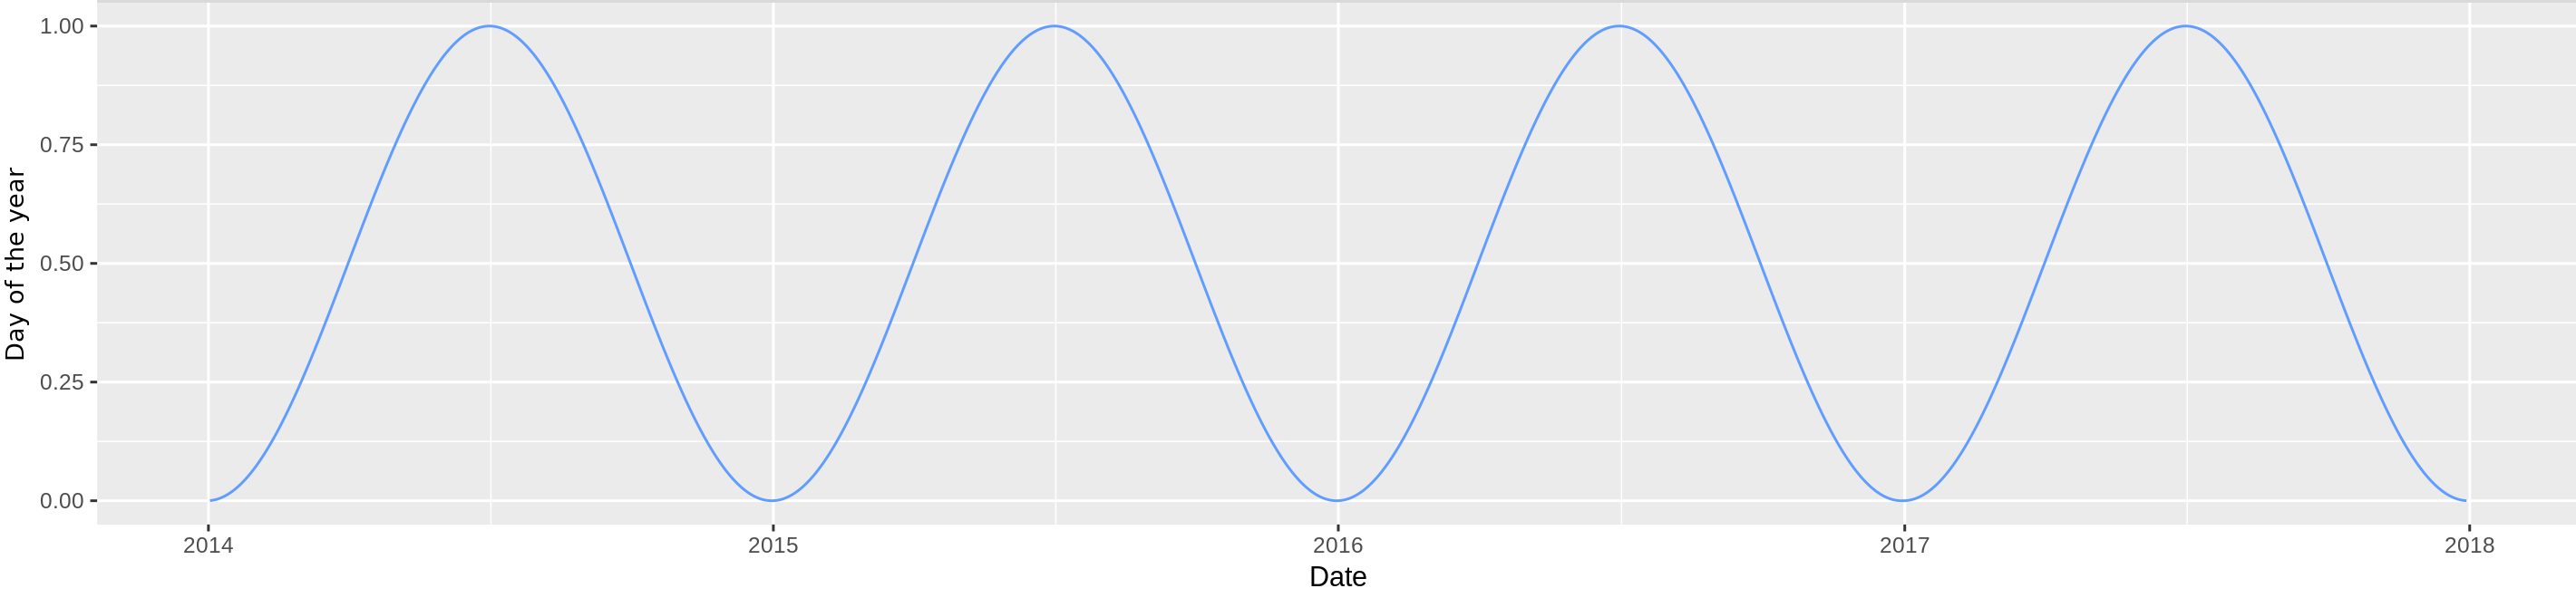
\includegraphics[width=\textwidth]{figures/dataset/fraction_of_period.png}
\caption{Result of the cosine transformation - day of the year}
\label{fig:dataset-cosine-transformation}
\end{figure}


\section{Anomaly detection}
The data set was tested for existence of measurements (\textit{outliers}) that do not match other observations registered in similar conditions. The process of eliminating them consisted of two steps:
\begin{enumerate}
    \item filtering out observations with values too extreme for climate that Krakow is located in - chosen thresholds are presented in table \ref{tab:dataset-anomaly-thresholds},
    \item analysis of histograms of each variable prepared for specific month and year and removing values that are relatively large/small and, at the same time, more frequent than the neighbouring ones.
\end{enumerate}

\begin{table}[H]
\centering
\caption{Thresholds used for anomaly detection}
\label{tab:dataset-anomaly-thresholds}
\begin{tabular}{llrr}
\toprule
Variable               & Units       & Lower threshold & Upper threshold \\ \midrule
Air humidity           & $\%$        & 0               & 100             \\
Air pressure           & $hPa$       & 970             & 1050            \\
Precipitation rate/sum & $mm$        & 0               & -               \\
Temperature            & $\degree C$ & -25             & 40              \\ 
Wind direction         & $\degree$   & 0               & 360             \\
Wind speed             & $m/s$       & 0               & -               \\ 
\bottomrule
\end{tabular}
\end{table}

\section{Missing data}
The air quality data were found to be incomplete with the number of missing PM2.5 concentrations ranging from 1.65\% to 3.27\%, depending on the station (table \ref{tab:dataset-missing-pm25}). Missing values were approximated using the Multiple Imputation by Chained Equations method \cite{MICE2011}, which is based on the idea of estimating the distribution of a specific variable based on the available data and drawing samples from that distribution (\textit{Gibbs sampling}). The decision of applying an imputation method instead of simply omitting the lacking records was taken in order to make the data set suitable for models that require the time series to be continuous e.g. ARIMA.

\begin{table}[H]
\centering
\caption{Percentage of missing PM2.5 measurements per station}
\label{tab:dataset-missing-pm25}
\begin{tabular}{lr}
\toprule
Station           & Missing PM2.5 {[}\%{]} \\ \midrule
GIOŚ Bujaka       & 2.920                  \\
GIOŚ Bulwarowa    & 3.271                  \\
GIOŚ Krasińskiego & 1.648                  \\ \bottomrule
\end{tabular}
\end{table}

\section{Data statistics}
After finishing the preprocessing steps, monthly means and standard deviations were calculated for the main variables used in this study: PM2.5, air humidity, total precipitation, air pressure, temperature, wind direction and speed. Results are presented in tables \ref{tab:dataset-stats-bujaka} - \ref{tab:dataset-stats-krasinskiego}, separately for each station.
\\\\
Figures \ref{fig:dataset-trend-pm25} - \ref{fig:dataset-trend-wind-speed} depict daily mean values of the variables. Some of them display strong seasonality: PM2.5 levels are highest in winter and lowest during summer, while temperatures and daily total precipitation show the opposite behaviour: they are highest during summer and lowest in winter. Humidity levels peak in autumn and reach lowest values during summer. 
\\\\
In the case of pressure, wind direction and speed one can notice that mean values increase with time, for example: pressure measured by stations Bujaka and Krasińskiego in 2014 tends to reach lower levels than in 2017. It is probably caused by mixing measurements from different sources in the case of activating a new weather sensor located closer to the air quality station.
\\\\
Scatter plots \ref{fig:dataset-bivariate-bujaka} - \ref{fig:dataset-bivariate-krasinskiego} depict relationships between the concentrations of PM2.5 at the moment T + 24 hours and the main explanatory variables mentioned in the previous paragraphs. They seem to be similar for all of the monitoring stations. Wind speed, total precipitation and, to some extent, temperature and humidity, display fairly strong nonlinear relationships with future PM2.5 levels. Dispersion of the PM2.5 concentrations for the same value of the predictor might be significant, however their maximum levels seem to be limited by nonlinear functions of the weather factors. PM2.5 concentrations, on the other hand, show a weak linear dependency on future PM2.5 levels - points on the scatter plots form cones, rather than lines. In the case of wind direction the widest range of PM2.5 levels corresponds roughly to 90$\degree$ and 270$\degree$, which is probably indicative of the fact that in Krakow West and East winds are the most common. 
\\\\
Table \ref{tab:dataset-correlation-significant} contains a ranking of the variables ordered by the corresponding absolute value of the Pearson correlation coefficient. The comparison was prepared separately for each of the monitoring stations and seasons. In each case the first position on the list is occupied by PM2.5 concentrations, while next variables vary, depending on the season. For winter they are: temperature, pressure and wind speed, for spring: day of the year, month, heating season, temperature and the period of the day, for summer: wind speed, day of year, pressure and month and for autumn: wind speed, pressure, temperature, day of the year and month.
\begin{landscape}
\begin{table}[H]
\centering
\caption{Variable statistics - GIOŚ Bujaka}
\label{tab:dataset-stats-bujaka}
\footnotesize
\begin{tabular}{llrrrrrrrrrrrrr}
\hline
Month & \multicolumn{2}{c}{PM2.5} & \multicolumn{2}{c}{Humidity} & \multicolumn{2}{c}{Total precipitation} & \multicolumn{2}{c}{Pressure} & \multicolumn{2}{c}{Temperature} & \multicolumn{2}{c}{Wind direction} & \multicolumn{2}{c}{Wind speed} \\
Units & \multicolumn{2}{c}{$\mu g / m^3$} & \multicolumn{2}{c}{$\%$} & \multicolumn{2}{c}{$mm$} & \multicolumn{2}{c}{$hPa$} & \multicolumn{2}{c}{$\degree C$} & \multicolumn{2}{c}{$\degree$} & \multicolumn{2}{c}{$m/s$} \\
Type & mean & std & mean & std & mean & std & mean & std & mean & std & mean & std & mean & std \\ \hline
January & 66.15 & 65.510 & 71.31 & 15.25 & 0.2052 & 0.7041 & 1004 & 17.38 & -0.5669 & 5.655 & 197.2 & 80.85 & 1.784 & 1.575 \\
February & 54.88 & 49.481 & 74.73 & 14.45 & 0.3133 & 1.0124 & 1007 & 15.34 & 3.1434 & 4.474 & 204.0 & 76.31 & 1.612 & 1.707 \\
March & 39.36 & 37.173 & 67.76 & 18.24 & 0.4025 & 1.3471 & 1009 & 14.74 & 6.5556 & 4.403 & 196.1 & 82.74 & 1.907 & 1.677 \\
April & 23.19 & 17.813 & 64.06 & 18.76 & 0.7157 & 2.2453 & 1007 & 13.33 & 10.1336 & 5.850 & 212.6 & 74.19 & 1.922 & 1.556 \\
May & 16.22 & 9.709 & 68.09 & 19.16 & 0.8329 & 2.3249 & 1007 & 13.36 & 14.9760 & 5.193 & 199.3 & 78.65 & 1.614 & 1.261 \\
June & 13.84 & 8.355 & 60.63 & 17.74 & 1.0023 & 3.9264 & 1008 & 11.70 & 19.1260 & 5.282 & 210.3 & 71.78 & 1.756 & 1.468 \\
July & 11.13 & 6.721 & 63.03 & 18.90 & 1.2676 & 4.4290 & 1007 & 12.85 & 21.0025 & 5.316 & 214.9 & 70.83 & 1.681 & 1.427 \\
August & 15.13 & 9.839 & 63.30 & 18.45 & 1.1871 & 5.9126 & 1009 & 14.08 & 20.2478 & 5.766 & 205.9 & 72.24 & 1.345 & 1.108 \\
September & 16.81 & 11.083 & 72.49 & 17.36 & 1.2302 & 3.9272 & 1009 & 12.65 & 15.6200 & 5.529 & 195.0 & 79.44 & 1.516 & 1.302 \\
October & 30.30 & 25.019 & 77.46 & 13.06 & 0.8068 & 2.7478 & 1010 & 13.60 & 9.3803 & 4.633 & 196.1 & 77.04 & 1.537 & 1.753 \\
November & 41.13 & 38.661 & 77.88 & 11.34 & 0.5977 & 1.4971 & 1009 & 13.12 & 5.7905 & 4.535 & 204.7 & 70.16 & 1.373 & 1.590 \\
December & 42.92 & 41.027 & 74.92 & 14.16 & 0.3207 & 1.1101 & 1013 & 15.80 & 2.8558 & 4.422 & 220.8 & 60.25 & 2.344 & 2.493 \\ \hline
\end{tabular}
\end{table}
\end{landscape}

\begin{landscape}
\begin{table}[H]
\centering
\caption{Variable statistics - GIOŚ Bulwarowa}
\label{tab:dataset-stats-bulwarowa}
\footnotesize
\begin{tabular}{llrrrrrrrrrrrrr}
\hline
Month & \multicolumn{2}{c}{PM2.5} & \multicolumn{2}{c}{Humidity} & \multicolumn{2}{c}{Total precipitation} & \multicolumn{2}{c}{Pressure} & \multicolumn{2}{c}{Temperature} & \multicolumn{2}{c}{Wind direction} & \multicolumn{2}{c}{Wind speed} \\
Units & \multicolumn{2}{c}{$\mu g / m^3$} & \multicolumn{2}{c}{$\%$} & \multicolumn{2}{c}{$mm$} & \multicolumn{2}{c}{$hPa$} & \multicolumn{2}{c}{$\degree C$} & \multicolumn{2}{c}{$\degree$} & \multicolumn{2}{c}{$m/s$} \\
Type & mean & std & mean & std & mean & std & mean & std & mean & std & mean & std & mean & std \\ \hline

January & 57.97 & 51.12 & 69.52 & 25.12 & 0.36 & 0.92 & 1013.37 & 12.26 & 0.09 & 5.20 & 203.32 & 110.84 & 3.31 & 4.39 \\ 
February & 51.42 & 40.53 & 75.13 & 13.81 & 0.76 & 1.98 & 1014.18 & 10.20 & 3.32 & 4.15 & 191.45 & 117.19 & 2.32 & 3.37 \\ 
March & 38.41 & 30.73 & 69.52 & 16.96 & 0.67 & 1.86 & 1015.63 & 9.88 & 6.85 & 4.37 & 217.33 & 111.75 & 3.48 & 4.43 \\ 
April & 23.87 & 16.83 & 65.81 & 18.79 & 0.87 & 2.55 & 1013.73 & 6.30 & 10.43 & 5.63 & 229.04 & 92.69 & 3.47 & 4.22 \\ 
May & 17.81 & 11.30 & 67.64 & 18.66 & 1.15 & 3.35 & 1013.64 & 5.93 & 15.51 & 5.22 & 219.83 & 63.23 & 2.39 & 3.66 \\ 
June & 13.92 & 8.91 & 60.19 & 18.50 & 0.99 & 4.03 & 1014.39 & 5.50 & 19.62 & 5.39 & 227.61 & 57.52 & 1.64 & 2.32 \\ 
July & 13.09 & 7.67 & 64.69 & 18.77 & 1.33 & 3.98 & 1013.65 & 4.73 & 21.32 & 5.26 & 249.09 & 70.67 & 2.03 & 2.94 \\ 
August & 17.00 & 10.94 & 66.50 & 18.53 & 1.34 & 6.37 & 1016.08 & 4.00 & 20.79 & 5.89 & 256.25 & 69.42 & 1.15 & 1.79 \\ 
September & 19.12 & 12.50 & 74.88 & 15.88 & 1.31 & 4.15 & 1016.34 & 6.14 & 15.86 & 5.27 & 223.47 & 89.16 & 1.75 & 2.88 \\ 
October & 32.31 & 24.79 & 80.81 & 12.58 & 1.20 & 3.98 & 1018.17 & 6.87 & 9.65 & 4.58 & 213.50 & 93.90 & 2.48 & 5.29 \\ 
November & 43.56 & 38.29 & 82.70 & 10.50 & 0.71 & 1.69 & 1015.76 & 8.06 & 5.73 & 4.45 & 196.89 & 103.70 & 4.30 & 5.42 \\ 
December & 41.36 & 35.74 & 81.19 & 10.36 & 0.26 & 0.79 & 1020.75 & 9.67 & 2.79 & 4.23 & 241.93 & 88.31 & 5.77 & 6.94 \\ 
\bottomrule

\end{tabular}
\end{table}
\end{landscape}


\begin{landscape}
\begin{table}[H]
\centering
\caption{Variable statistics - GIOŚ Krasińskiego}
\label{tab:dataset-stats-krasinskiego}
\footnotesize
\begin{tabular}{llrrrrrrrrrrrrr}
\hline
Month & \multicolumn{2}{c}{PM2.5} & \multicolumn{2}{c}{Humidity} & \multicolumn{2}{c}{Total precipitation} & \multicolumn{2}{c}{Pressure} & \multicolumn{2}{c}{Temperature} & \multicolumn{2}{c}{Wind direction} & \multicolumn{2}{c}{Wind speed} \\
Units & \multicolumn{2}{c}{$\mu g / m^3$} & \multicolumn{2}{c}{$\%$} & \multicolumn{2}{c}{$mm$} & \multicolumn{2}{c}{$hPa$} & \multicolumn{2}{c}{$\degree C$} & \multicolumn{2}{c}{$\degree$} & \multicolumn{2}{c}{$m/s$} \\
Type & mean & std & mean & std & mean & std & mean & std & mean & std & mean & std & mean & std \\ \hline

January & 74.02 & 59.89 & 70.23 & 14.00 & 0.19 & 0.66 & 1003.02 & 18.43 & -0.12 & 5.31 & 185.90 & 86.92 & 2.76 & 2.28 \\ 
February & 67.75 & 47.65 & 73.16 & 14.41 & 0.26 & 0.81 & 1001.84 & 16.56 & 3.05 & 4.27 & 185.54 & 85.95 & 2.84 & 2.90 \\ 
March & 48.70 & 35.66 & 66.84 & 17.49 & 0.23 & 0.89 & 1002.43 & 14.58 & 6.44 & 4.35 & 189.08 & 87.86 & 2.91 & 2.51 \\ 
April & 33.18 & 20.50 & 64.50 & 18.99 & 0.35 & 1.40 & 1000.77 & 14.18 & 9.87 & 5.56 & 207.02 & 84.75 & 3.00 & 2.80 \\ 
May & 25.59 & 13.37 & 67.48 & 18.77 & 0.74 & 2.21 & 1001.47 & 14.54 & 14.96 & 5.62 & 188.57 & 90.29 & 2.65 & 2.24 \\ 
June & 19.89 & 10.20 & 62.02 & 18.21 & 0.89 & 3.89 & 1003.25 & 13.50 & 18.87 & 5.41 & 207.62 & 80.69 & 2.63 & 2.32 \\ 
July & 20.62 & 9.25 & 65.34 & 19.55 & 1.09 & 4.33 & 1001.32 & 13.89 & 20.66 & 5.23 & 214.11 & 76.03 & 2.34 & 2.01 \\ 
August & 23.91 & 12.44 & 65.54 & 19.48 & 1.01 & 4.40 & 1003.94 & 15.15 & 20.44 & 6.02 & 197.36 & 82.27 & 2.15 & 1.83 \\ 
September & 29.00 & 14.12 & 74.22 & 17.07 & 0.72 & 2.19 & 1004.31 & 14.55 & 15.35 & 5.48 & 184.36 & 89.38 & 2.50 & 2.40 \\ 
October & 44.48 & 28.44 & 82.15 & 15.04 & 0.46 & 1.71 & 1005.63 & 14.06 & 8.96 & 4.62 & 179.76 & 86.95 & 2.55 & 2.69 \\ 
November & 58.54 & 42.27 & 81.85 & 13.53 & 0.32 & 1.06 & 1003.05 & 14.13 & 5.22 & 4.61 & 170.22 & 88.59 & 2.76 & 2.49 \\ 
December & 55.06 & 41.28 & 79.23 & 14.12 & 0.13 & 0.41 & 1007.78 & 15.57 & 2.31 & 4.48 & 214.18 & 72.72 & 4.13 & 3.43 \\ 
\bottomrule

\end{tabular}
\end{table}
\end{landscape}

% Yearly trends %

\begin{landscape}
\begin{figure}[htp]
\centering
  \centering
  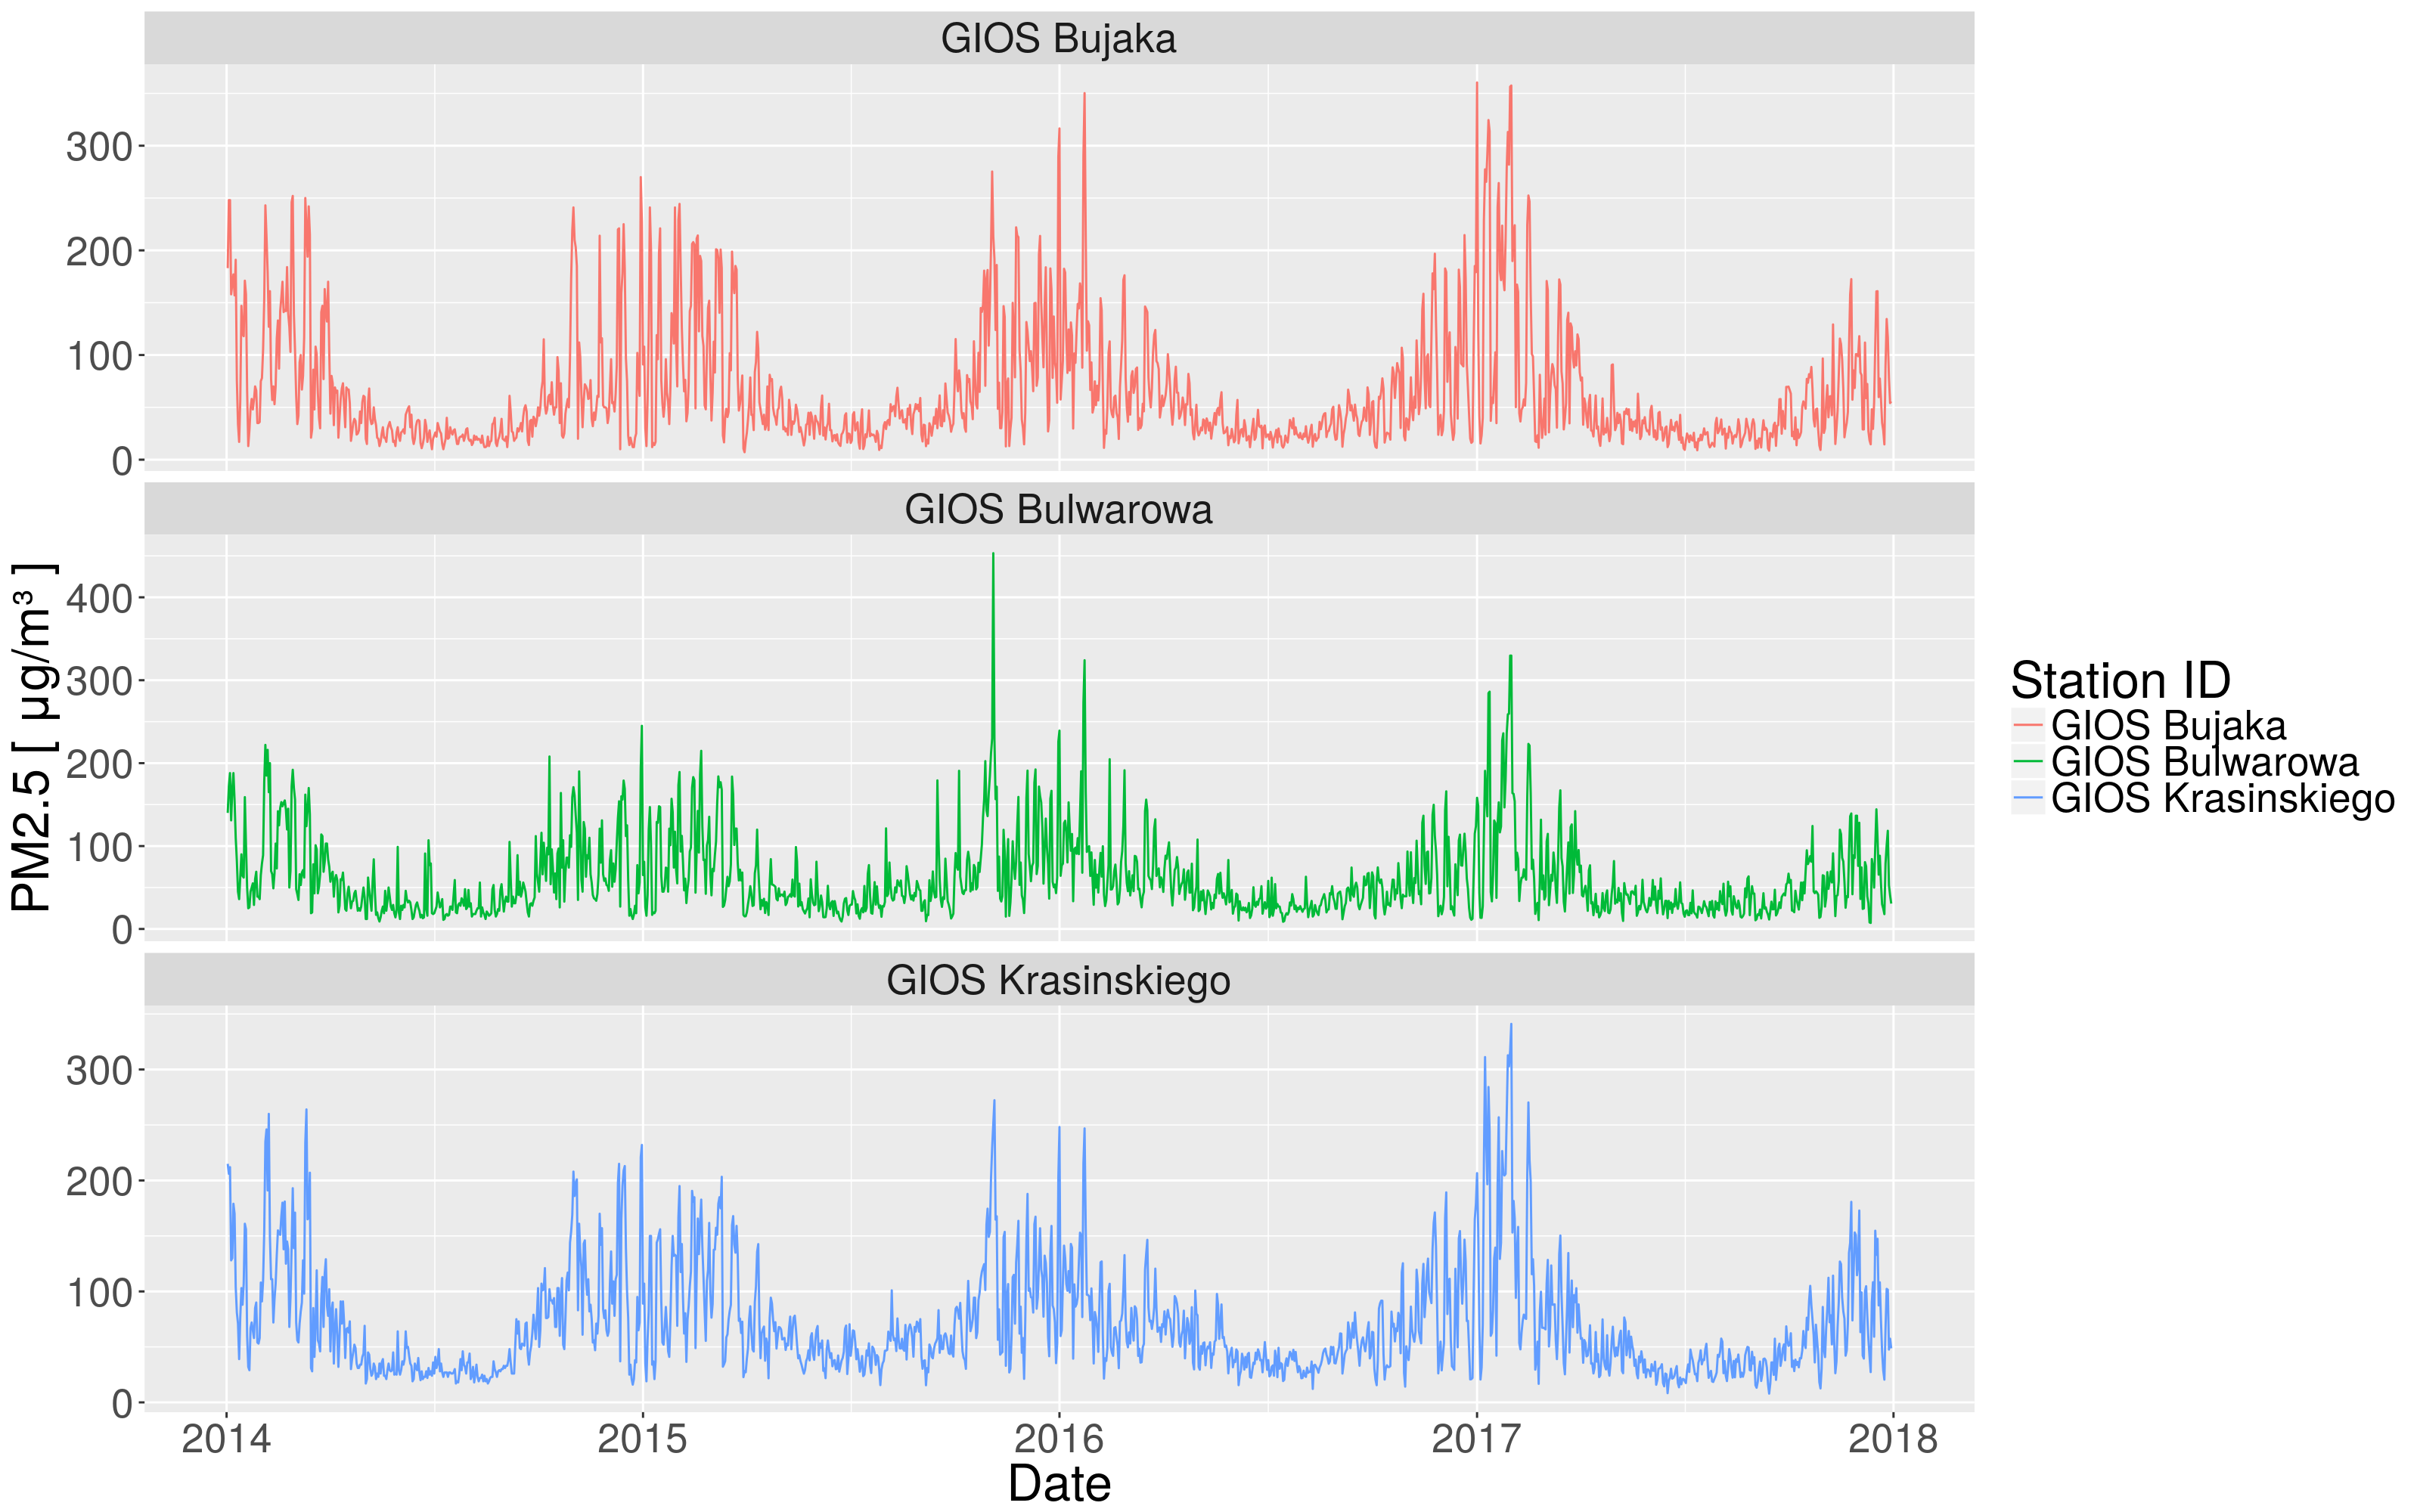
\includegraphics[width=\linewidth]{figures/dataset/trend/pm2_5_yearly_trend.png}
  \caption{Mean daily PM2.5 concentrations}
  \label{fig:dataset-trend-pm25}
\end{figure}
\end{landscape}
\begin{landscape}
\begin{figure}[htp]
\centering
  \centering
  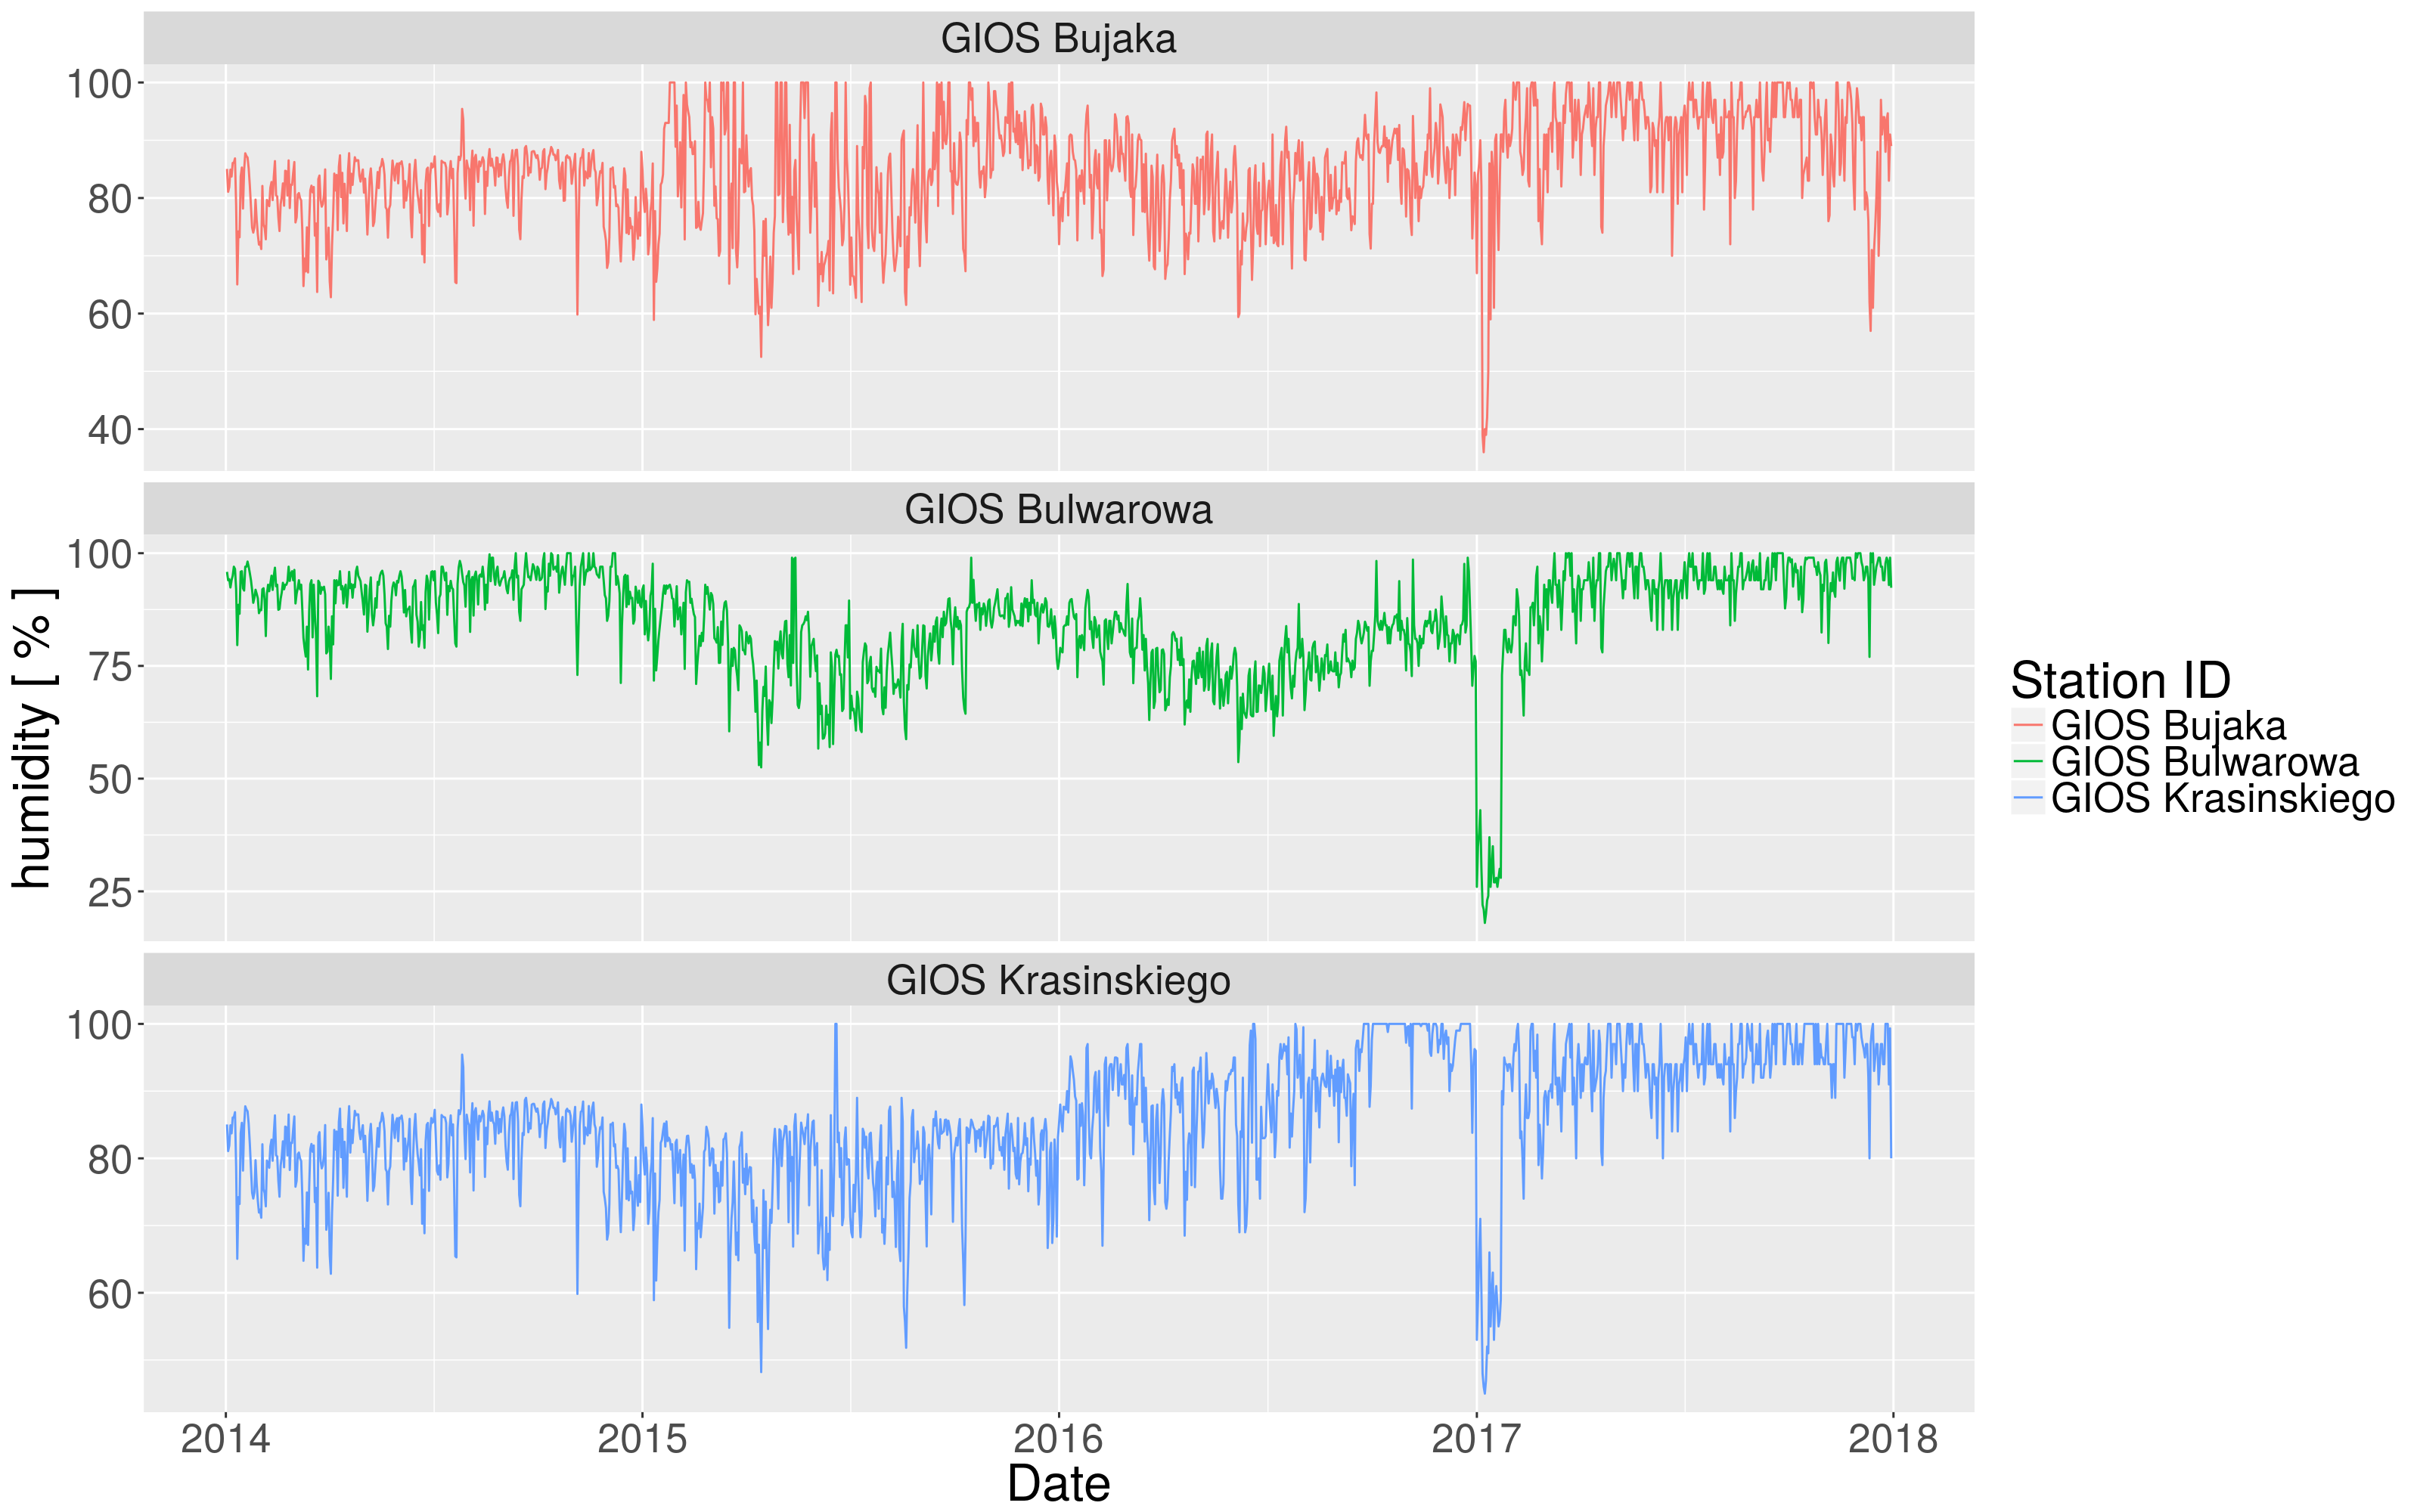
\includegraphics[width=\linewidth]{figures/dataset/trend/humidity_yearly_trend.png}
  \caption{Mean daily humidity}
  \label{fig:dataset-trend-humidity}
\end{figure}
\end{landscape}
\begin{landscape}
\begin{figure}[htp]
\centering
  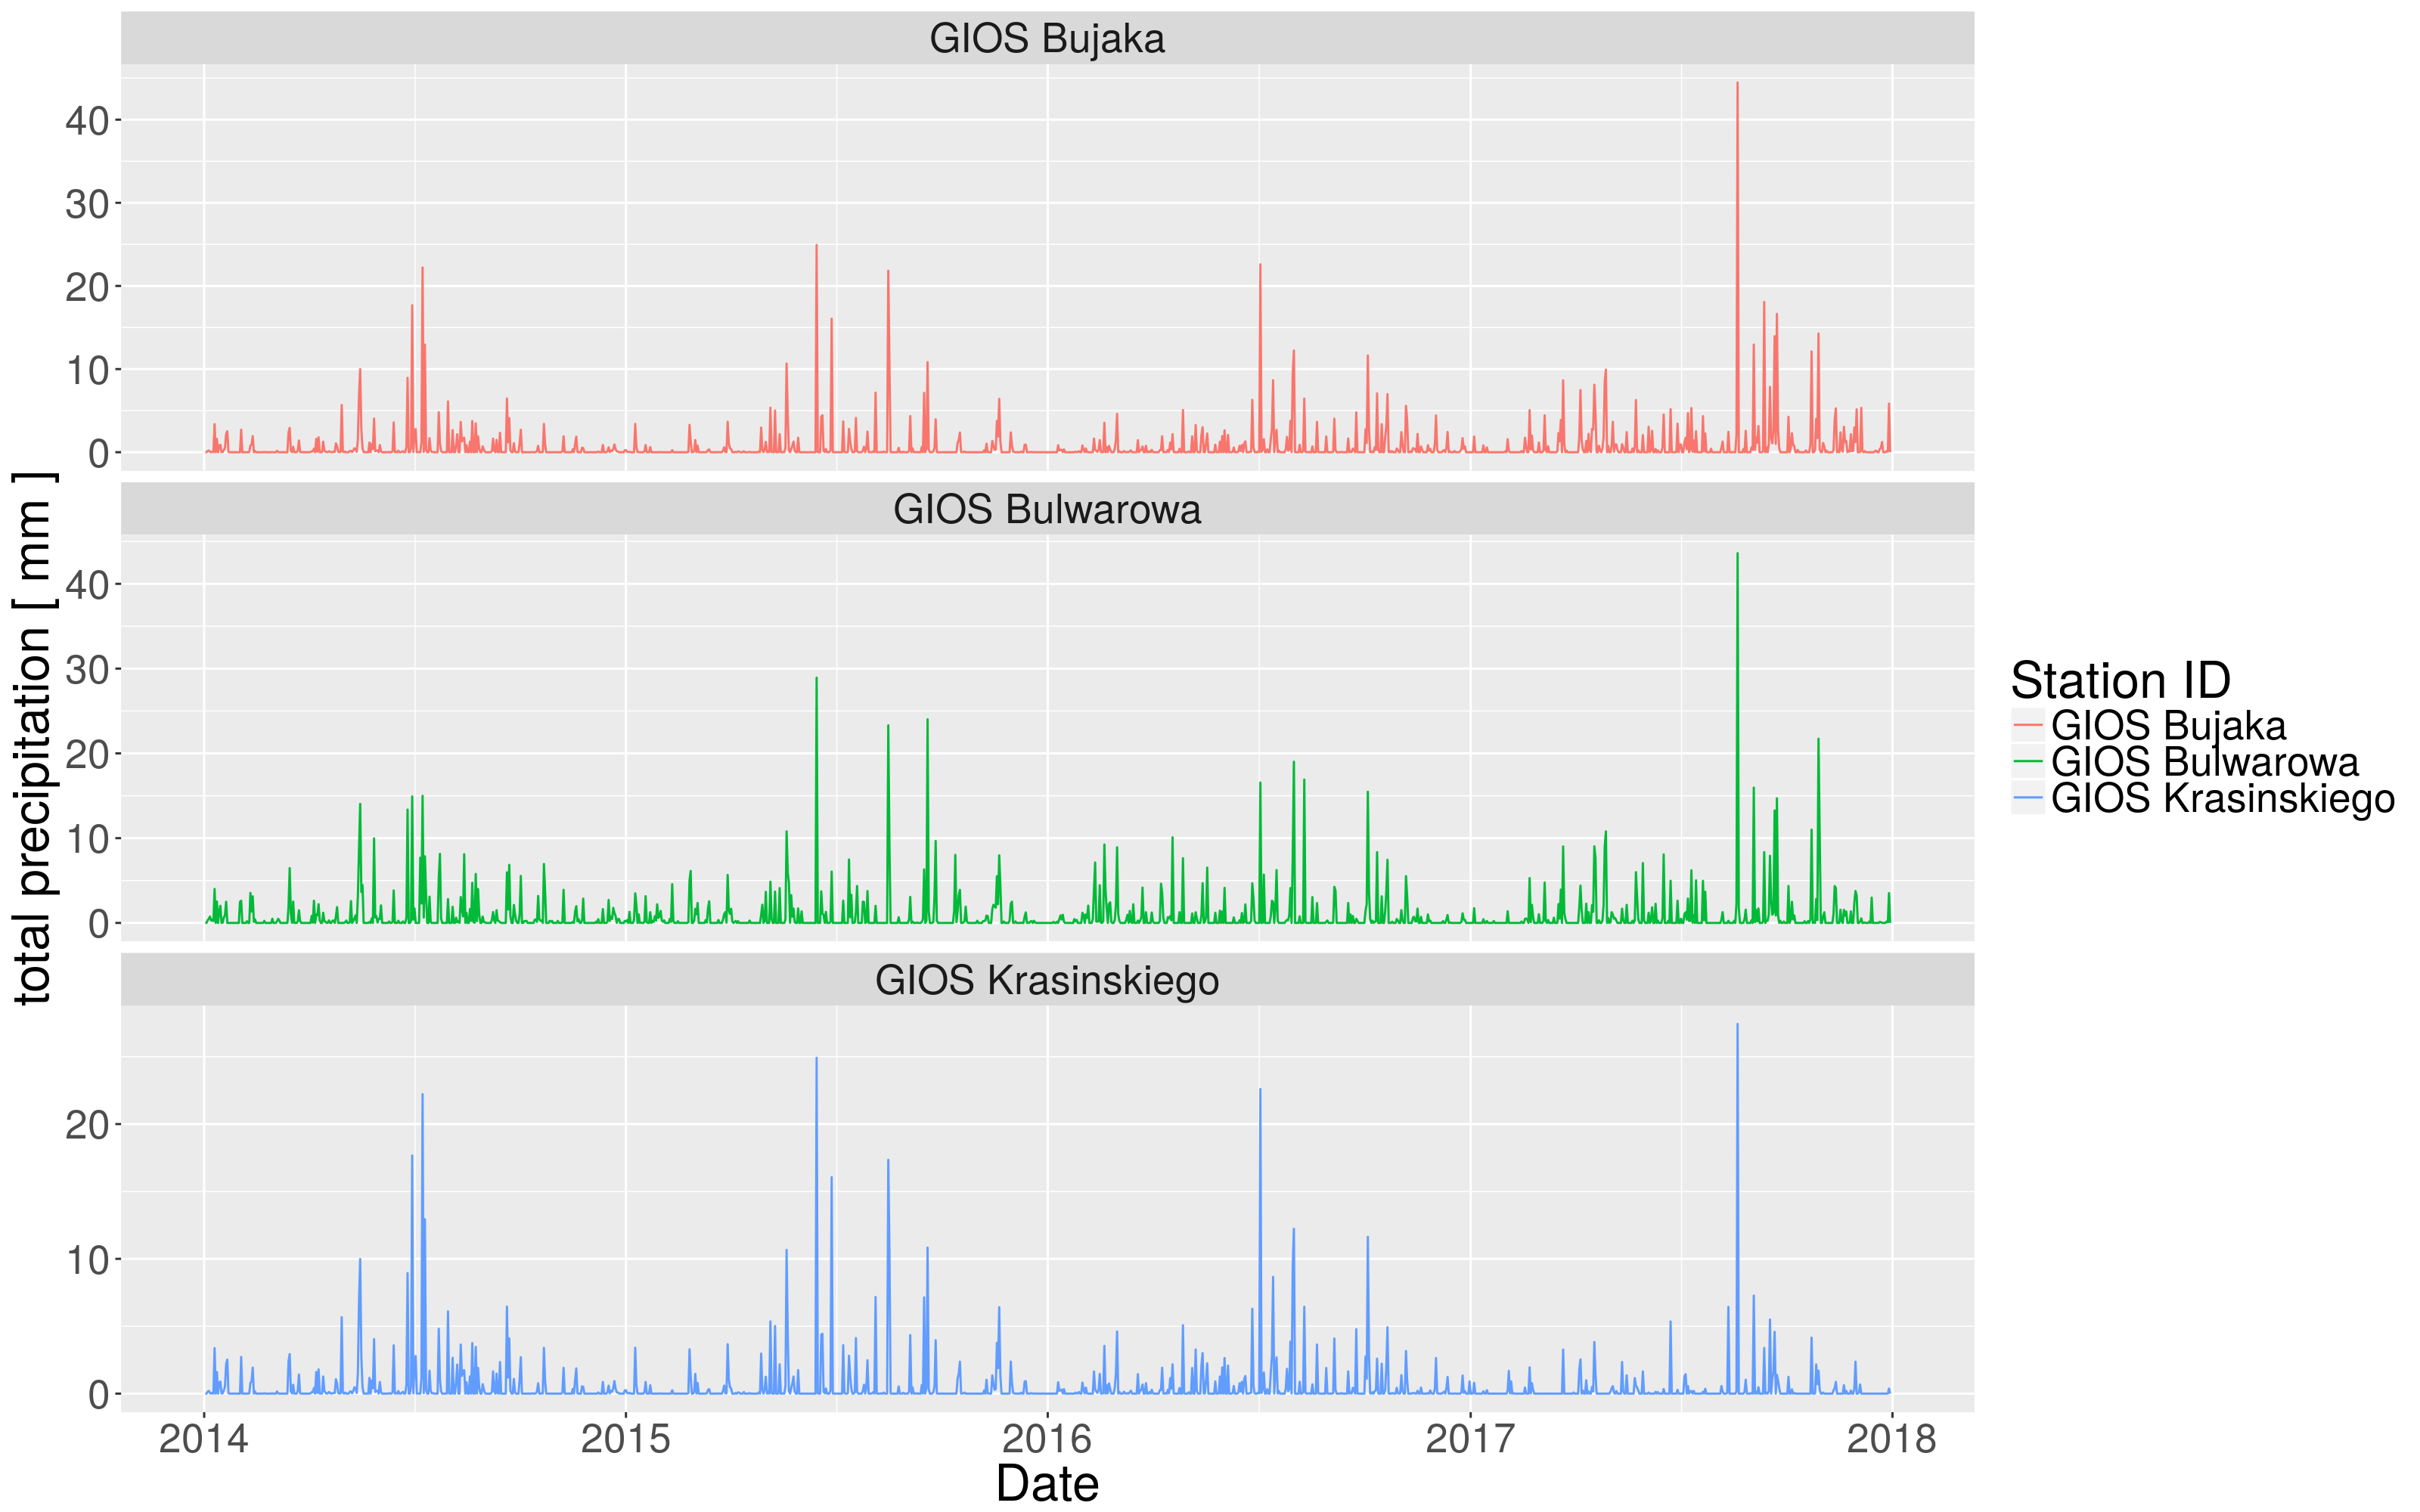
\includegraphics[width=\linewidth]{figures/dataset/trend/precip_total_yearly_trend.png}
  \caption{Daily total precipitation}
  \label{fig:dataset-trend-precip-total}
\end{figure}
\end{landscape}
\begin{landscape}
\begin{figure}[htp]
\centering
  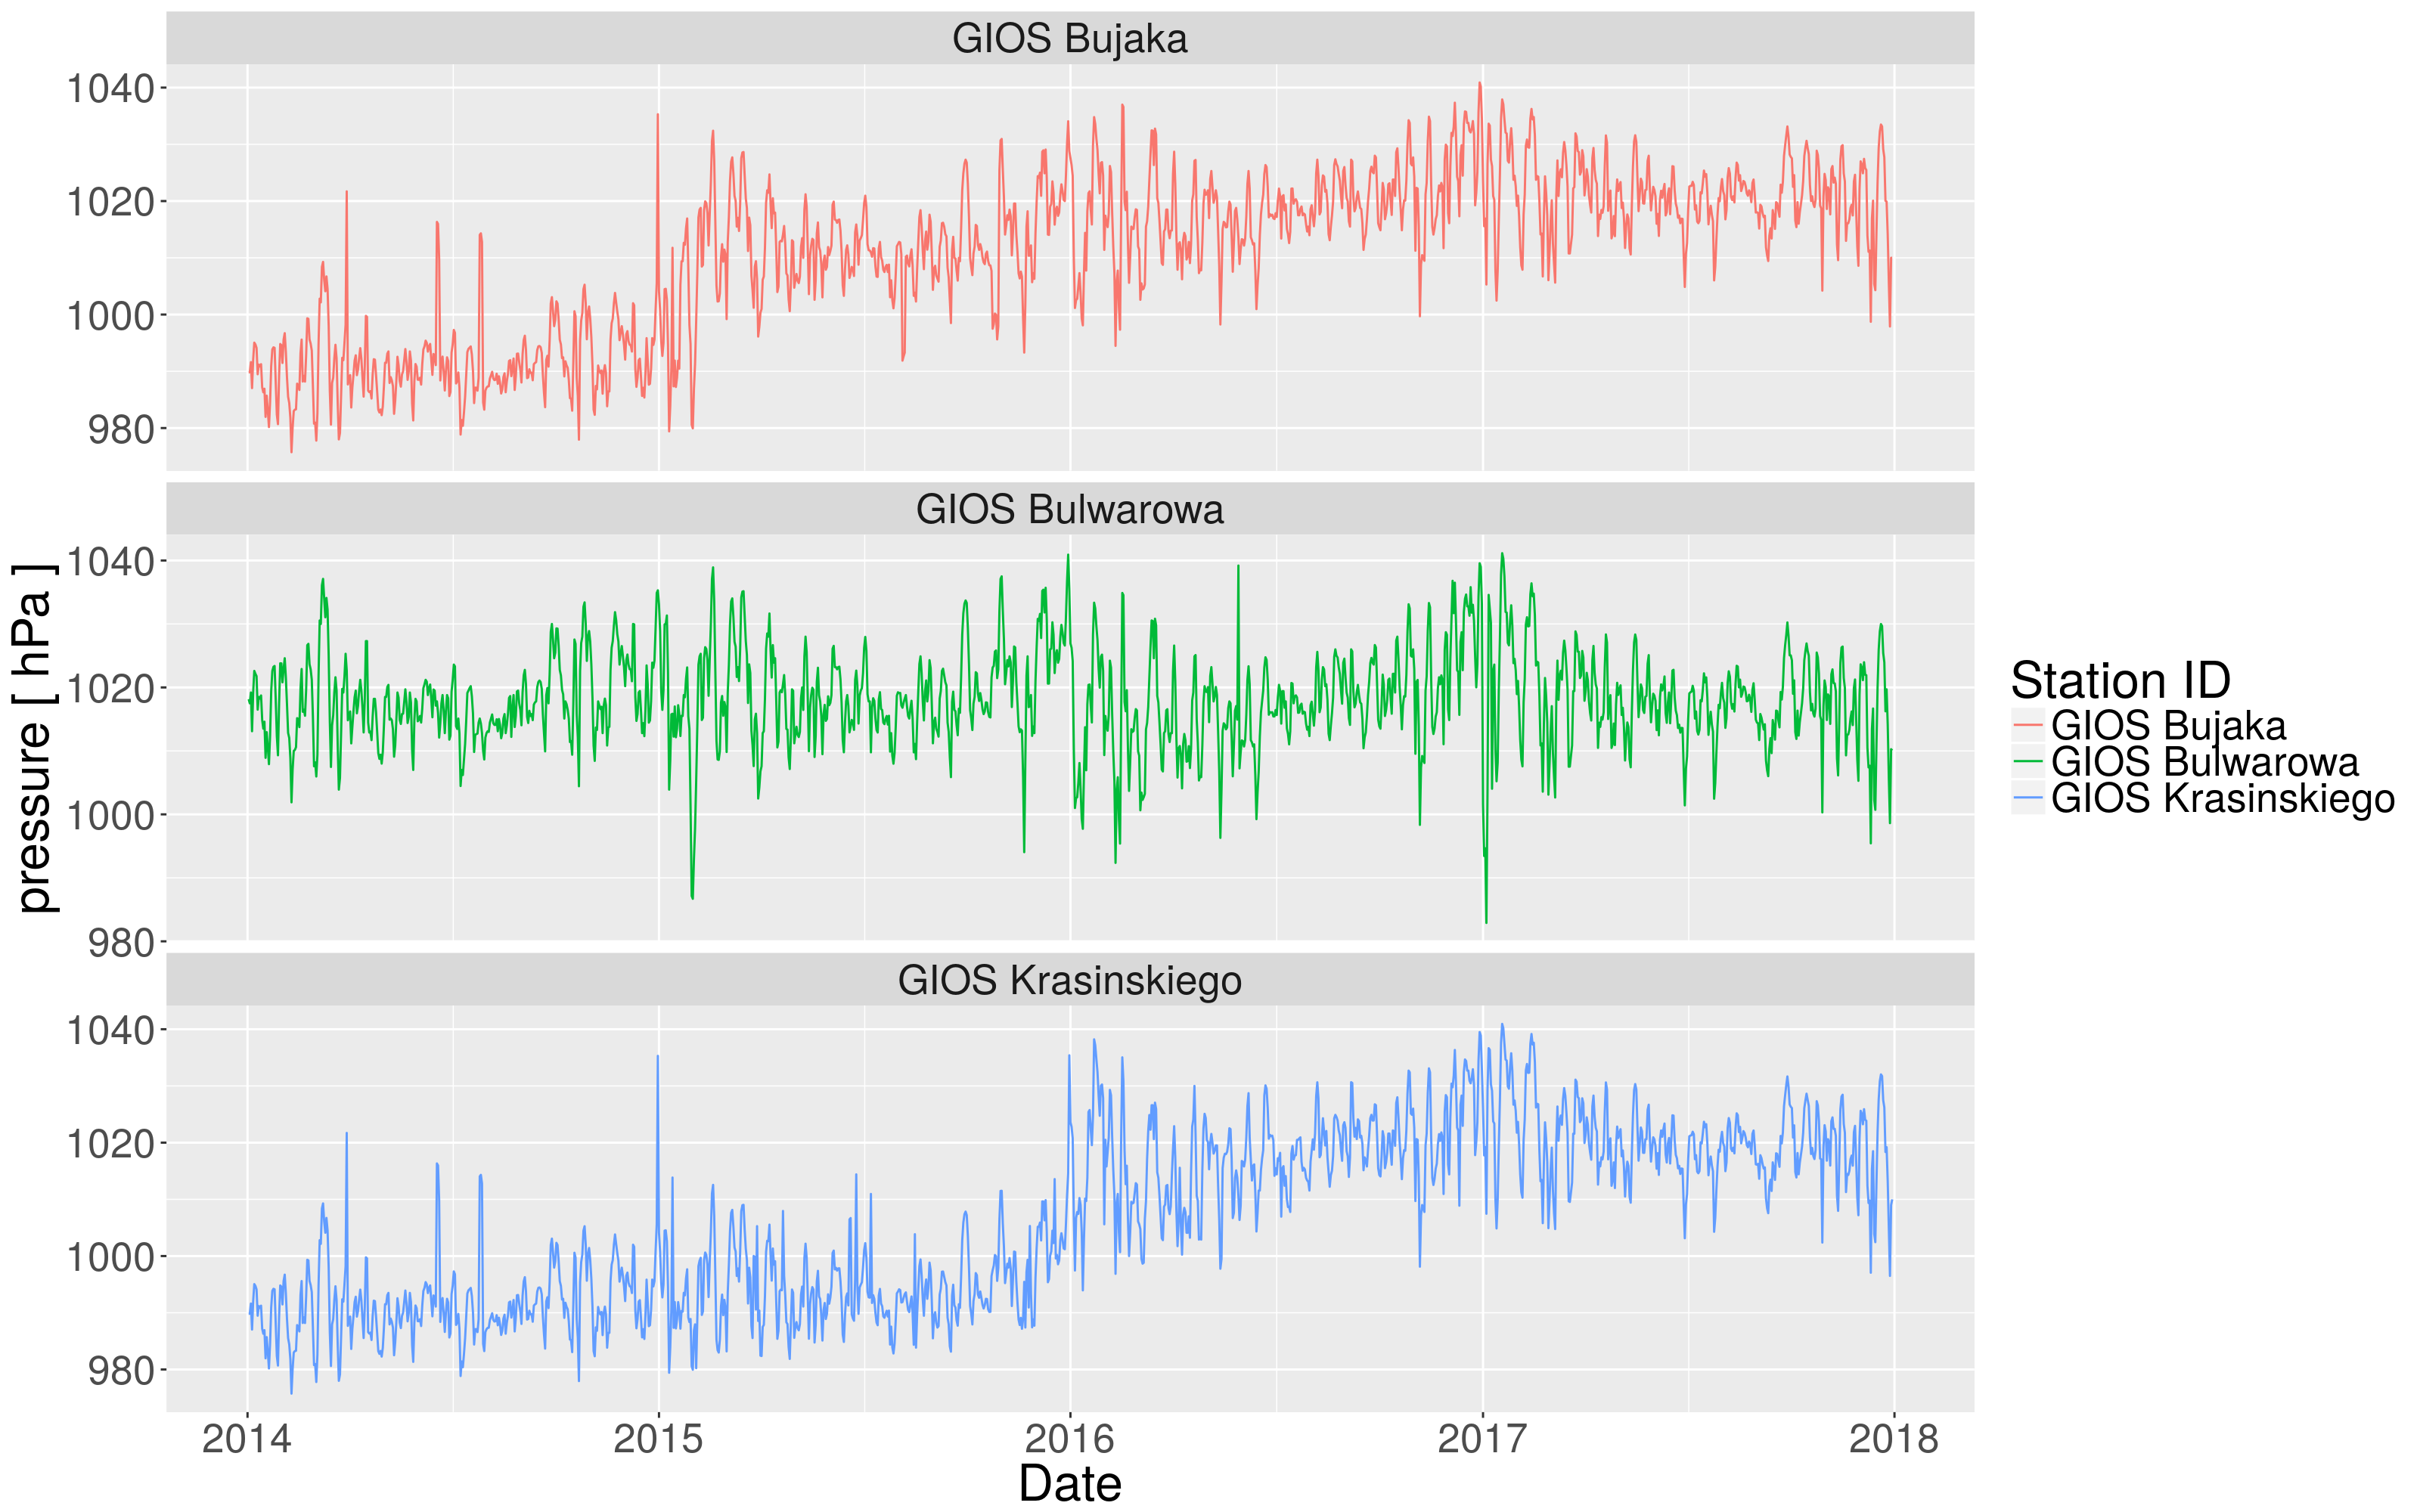
\includegraphics[width=\linewidth]{figures/dataset/trend/pressure_yearly_trend.png}
  \caption{Mean daily atmospheric pressure}
  \label{fig:dataset-trend-pressure}
\end{figure}
\end{landscape}
\begin{landscape}
\begin{figure}[htp]
\centering
  \centering
      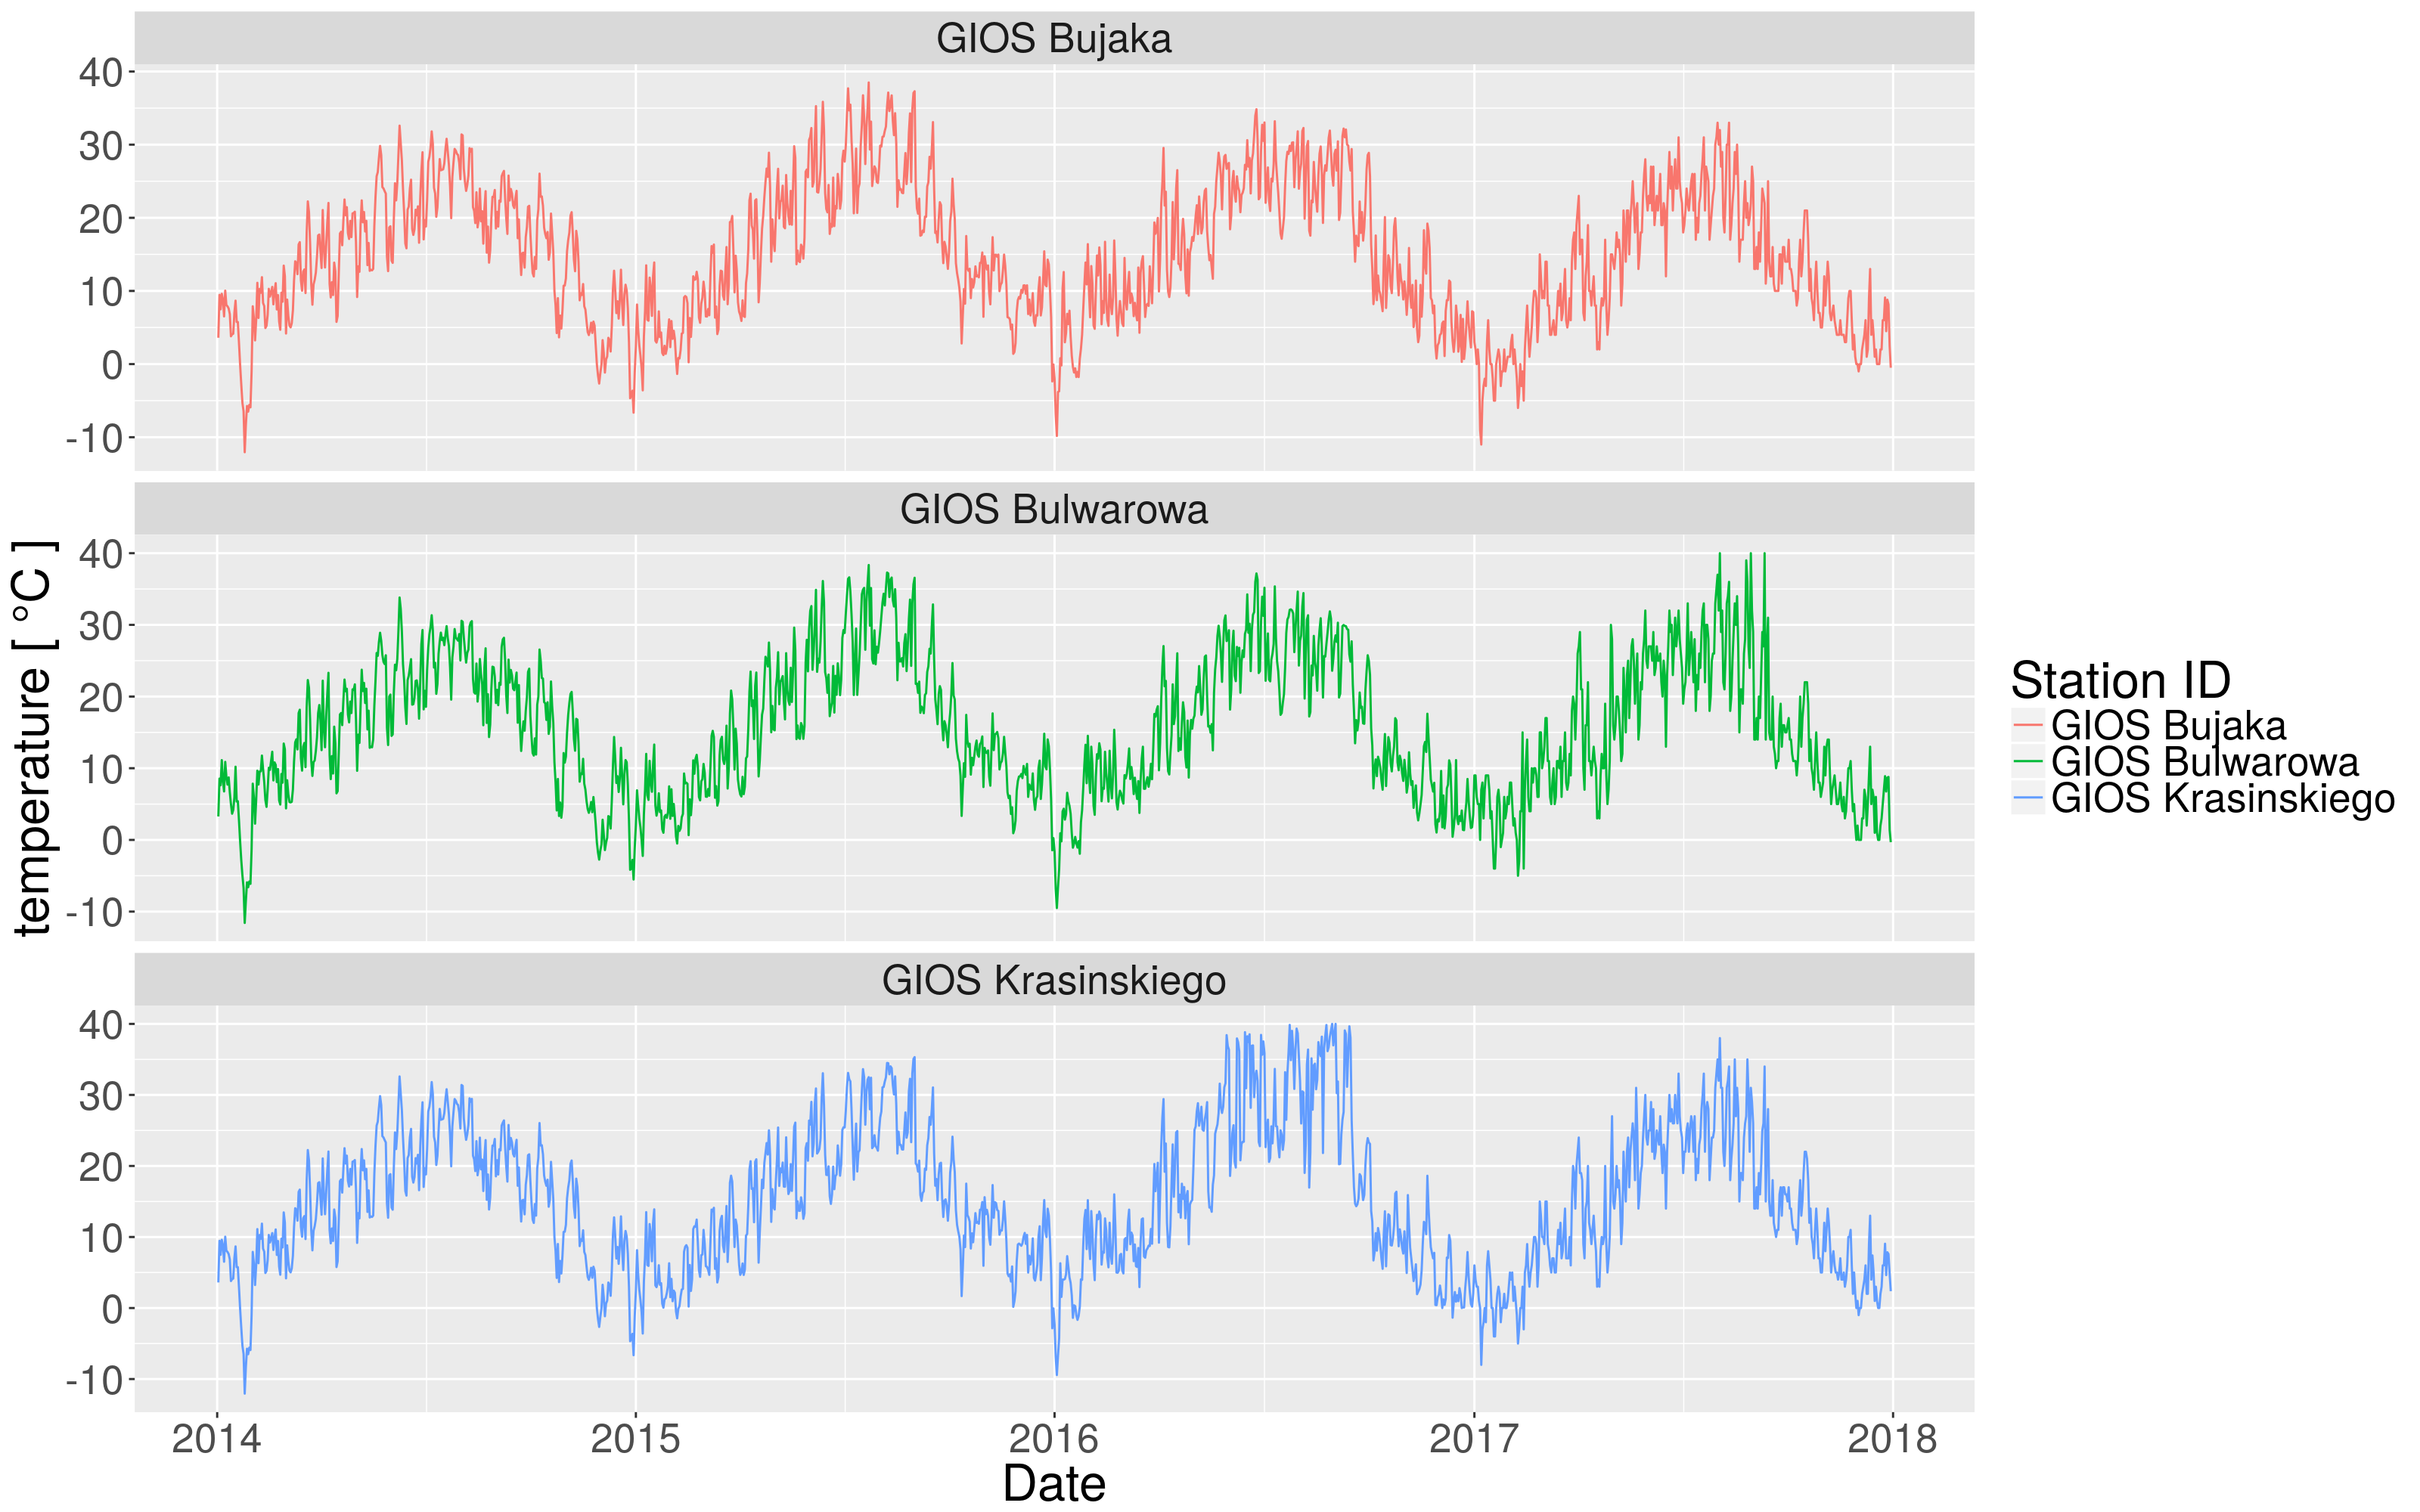
\includegraphics[width=\linewidth]{figures/dataset/trend/temperature_yearly_trend.png}
  \caption{Mean daily temperature}
  \label{fig:dataset-trend-temperature}
\end{figure}
\end{landscape}

\begin{landscape}
\begin{figure}[htp]
\centering
  \centering
  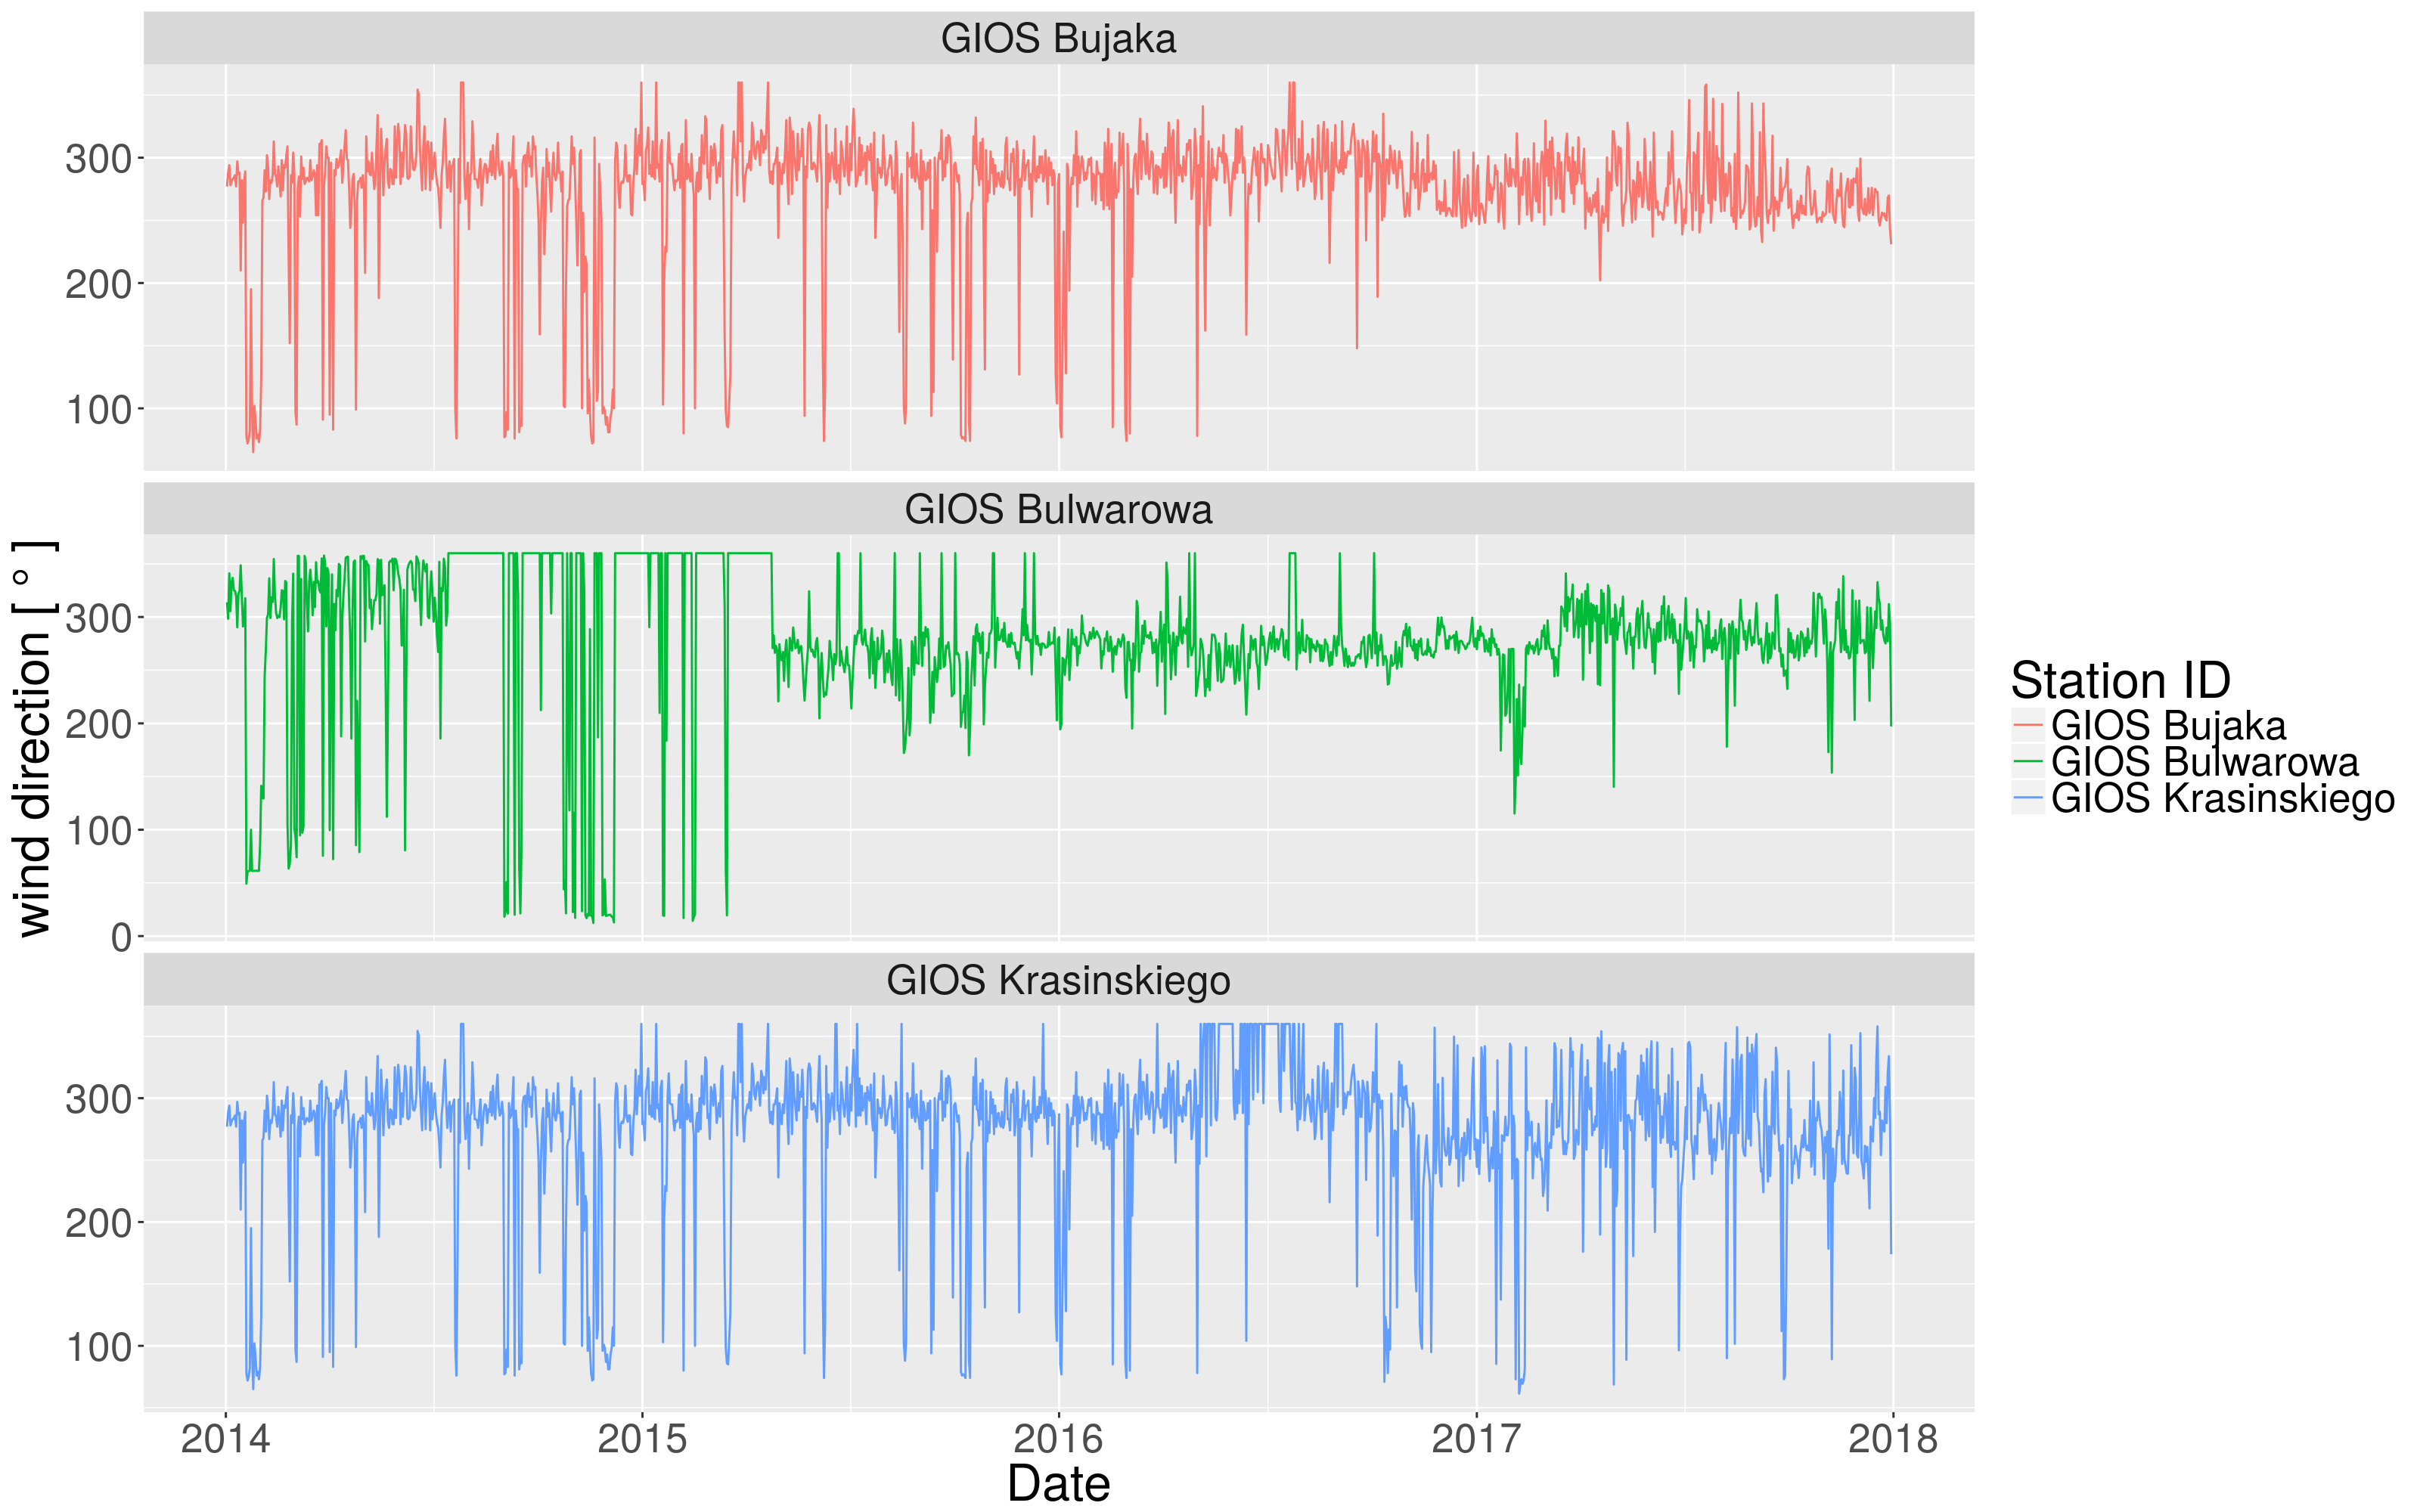
\includegraphics[width=\linewidth]{figures/dataset/trend/wind_dir_deg_yearly_trend.png}
  \caption{Mean daily wind direction}
  \label{fig:dataset-trend-wind-dir-ew}
  \end{figure}
\end{landscape}
\begin{landscape}
\begin{figure}[htp]
\centering
  \centering
  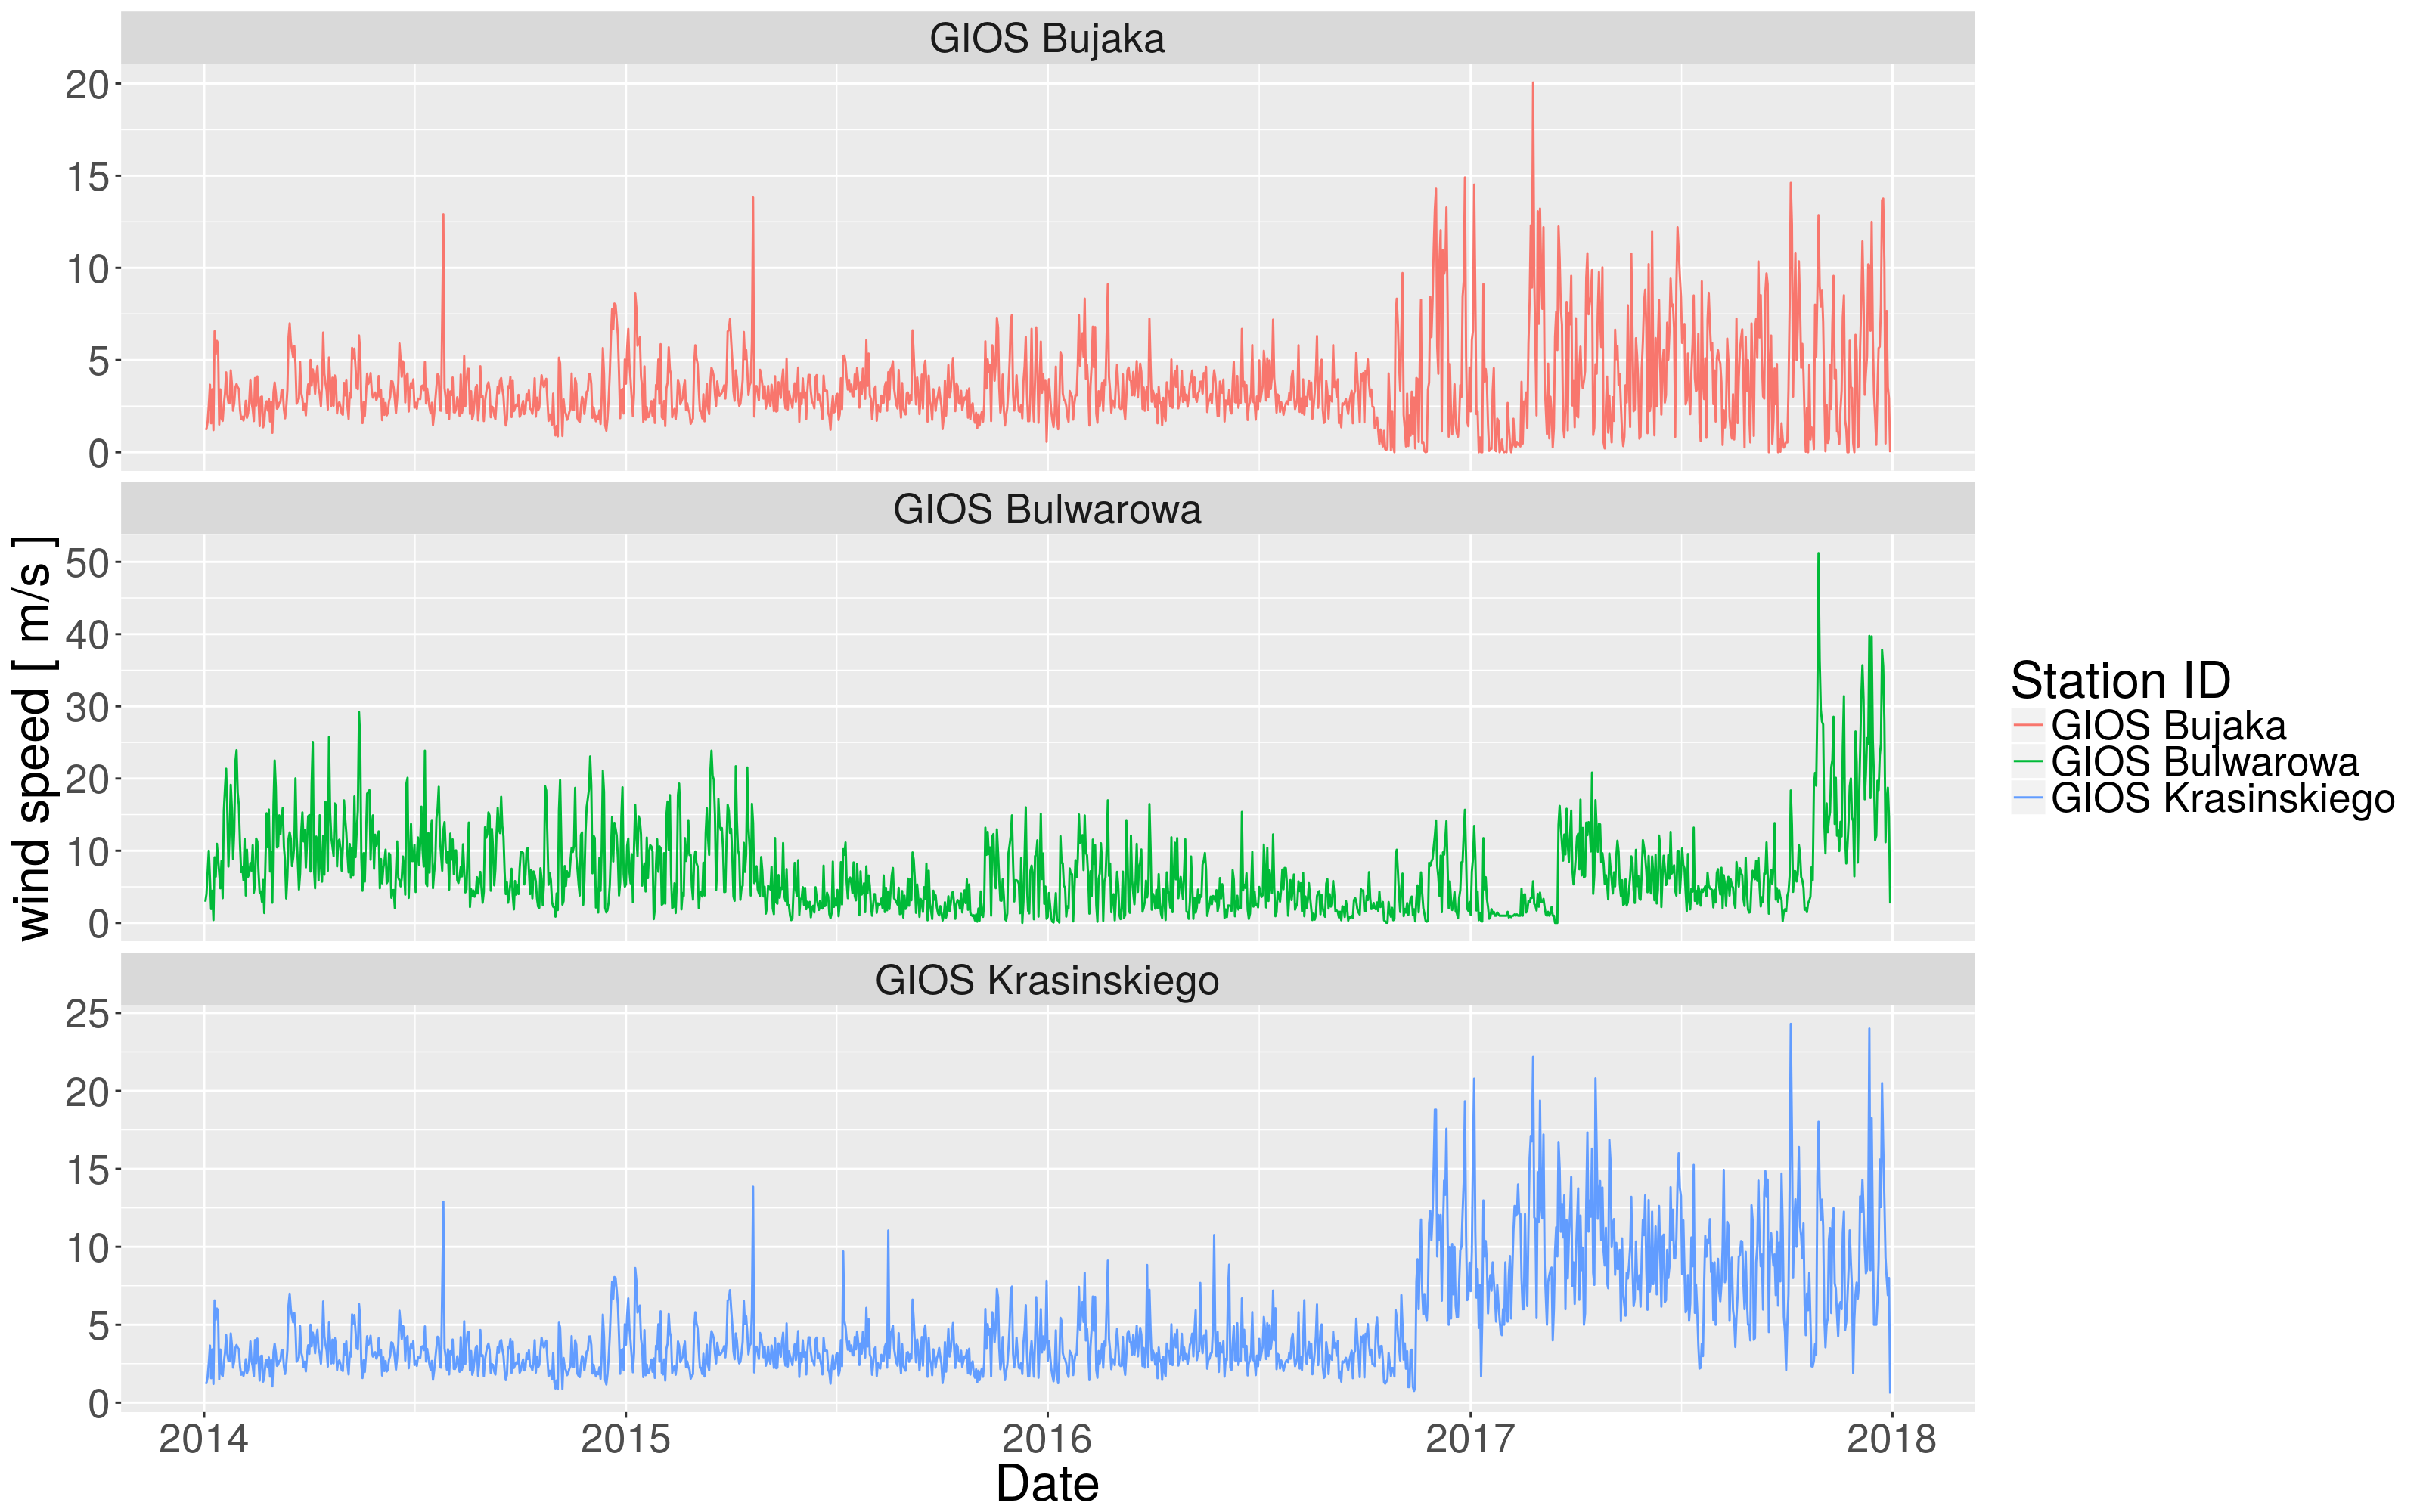
\includegraphics[width=\linewidth]{figures/dataset/trend/wind_speed_yearly_trend.png}
  \caption{Mean daily wind speed}
  \label{fig:dataset-trend-wind-speed}
  \end{figure}
\end{landscape}

% BI-VARIATE SCATTER PLOTS %

\begin{landscape}
\begin{figure}[htp]
\centering
  \centering
  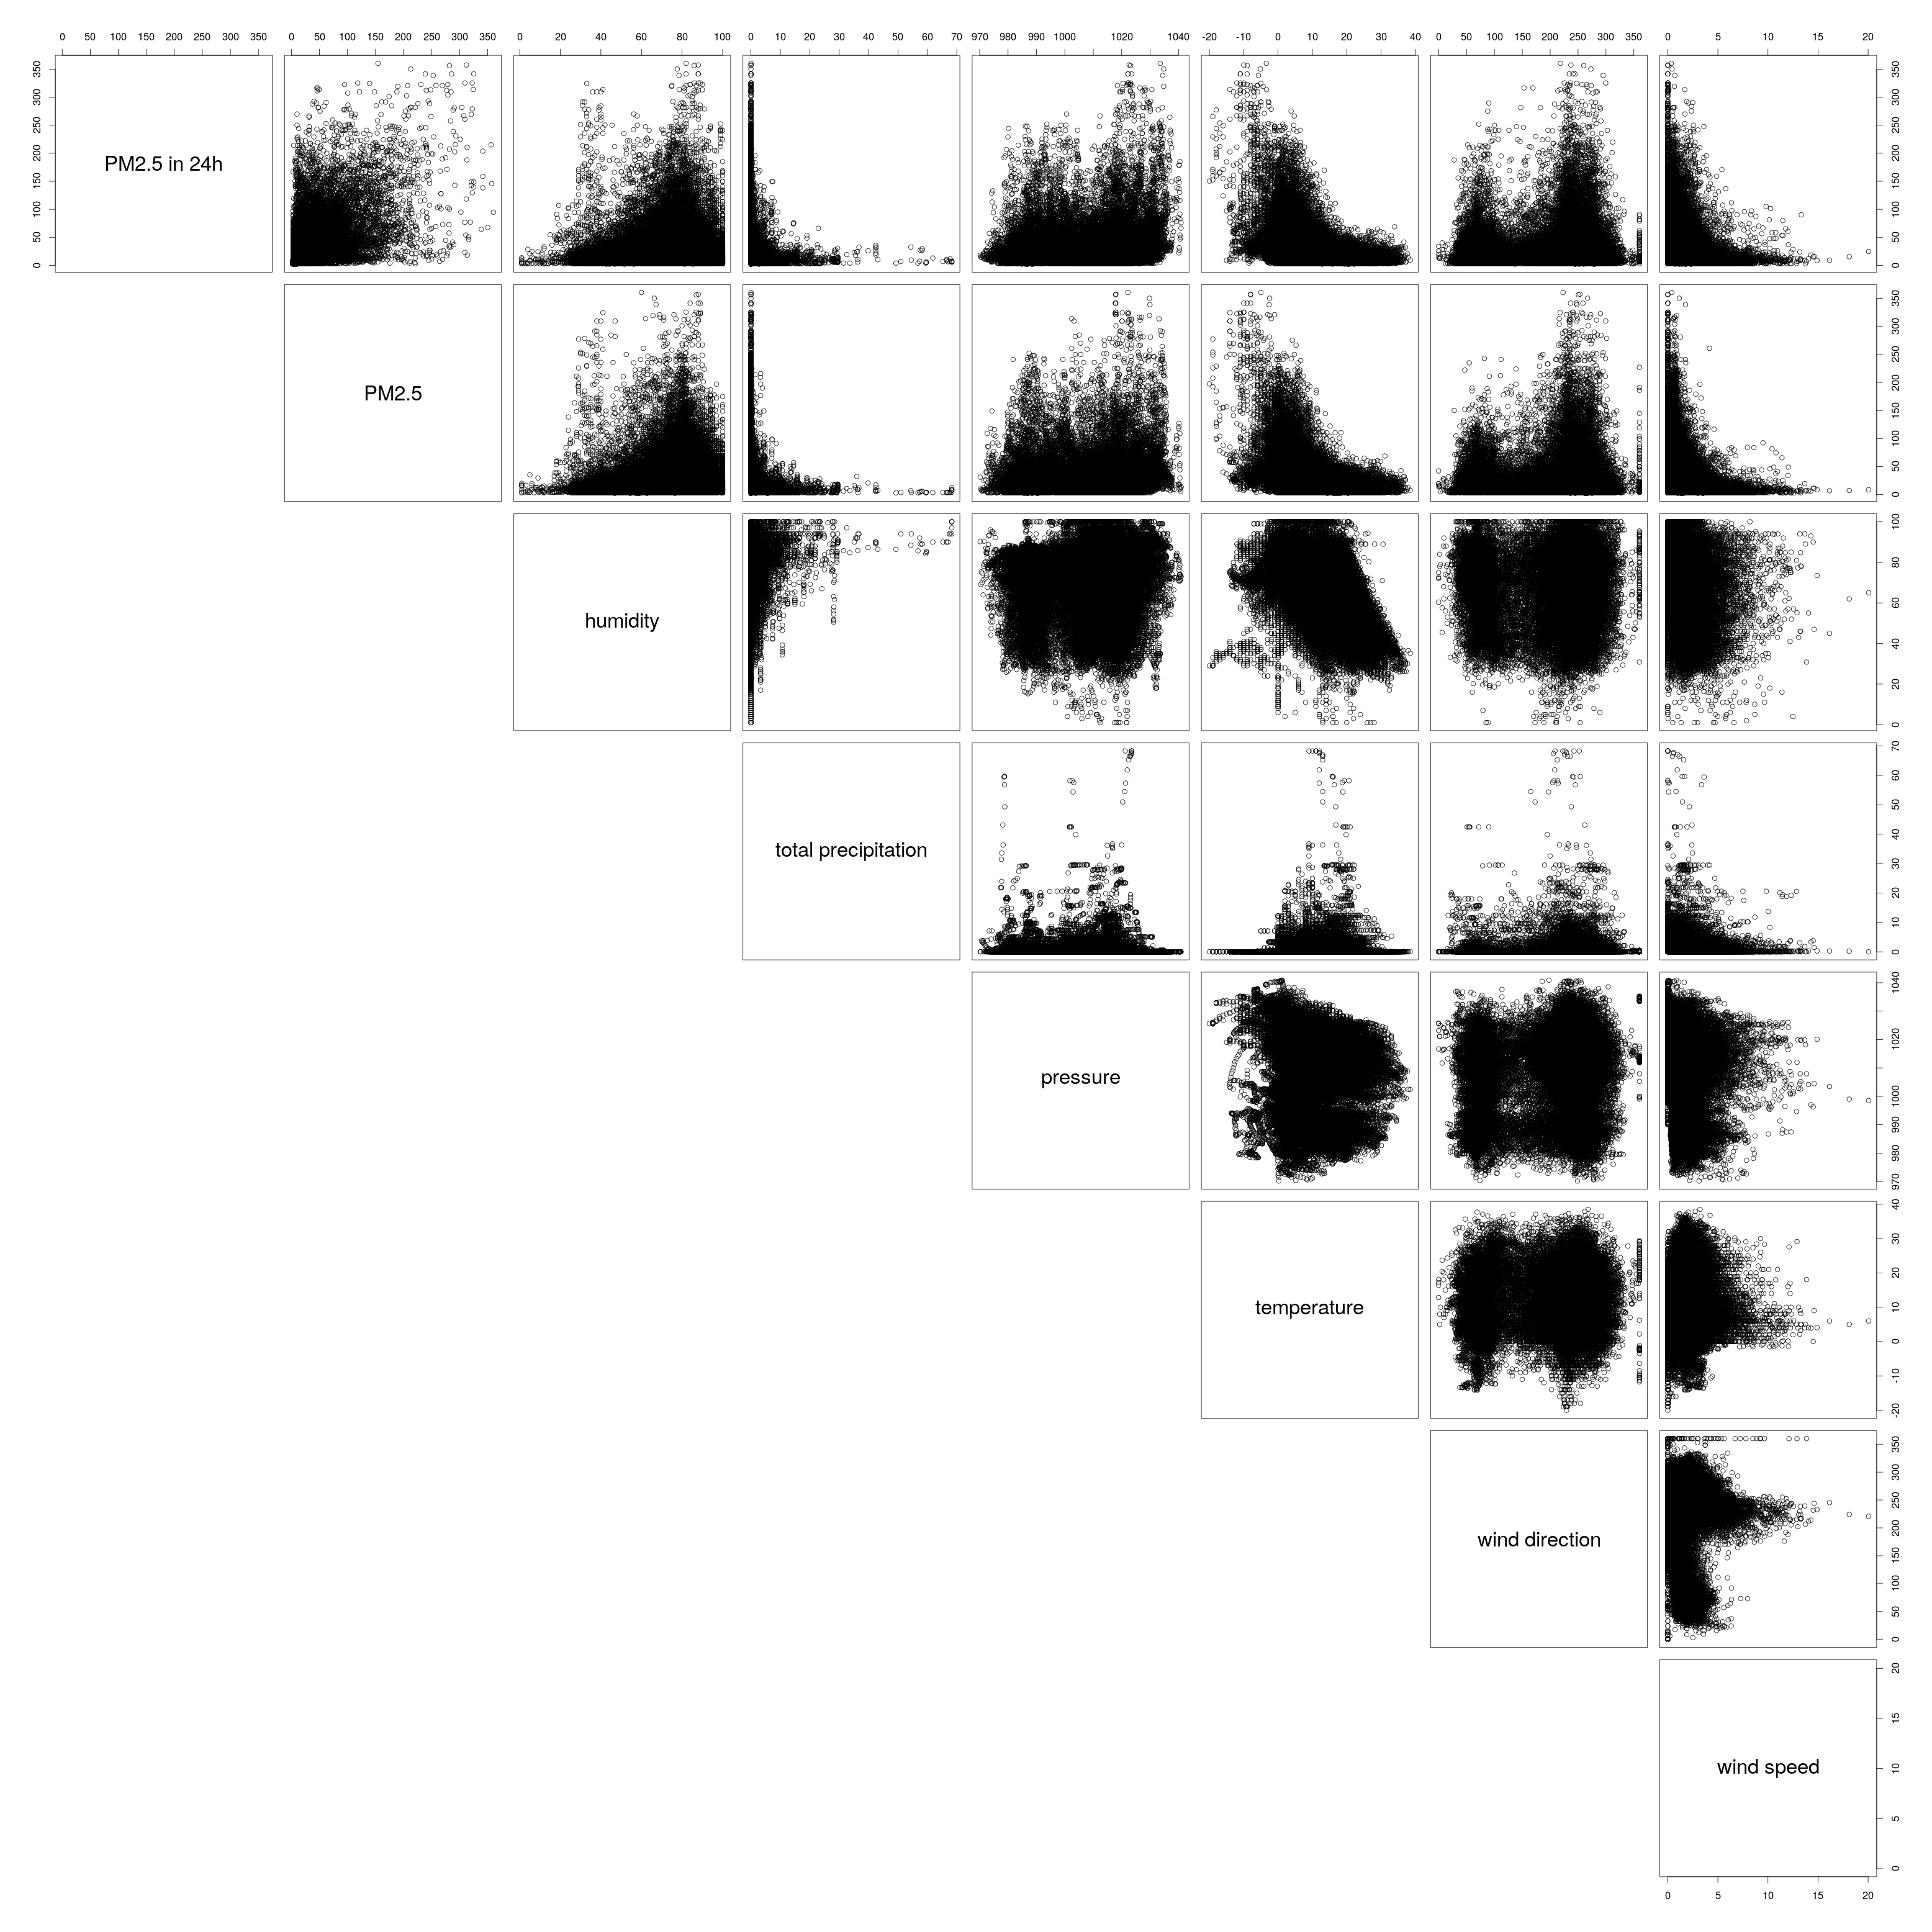
\includegraphics[width=0.65\linewidth]{figures/dataset/bivariate/relationships_gios_bujaka.png}
  \caption{Bivariate relationships - GIOŚ Bujaka}
  \label{fig:dataset-bivariate-bujaka}
\end{figure}
\end{landscape}
\begin{landscape}
\begin{figure}[htp]
\centering
  \centering
    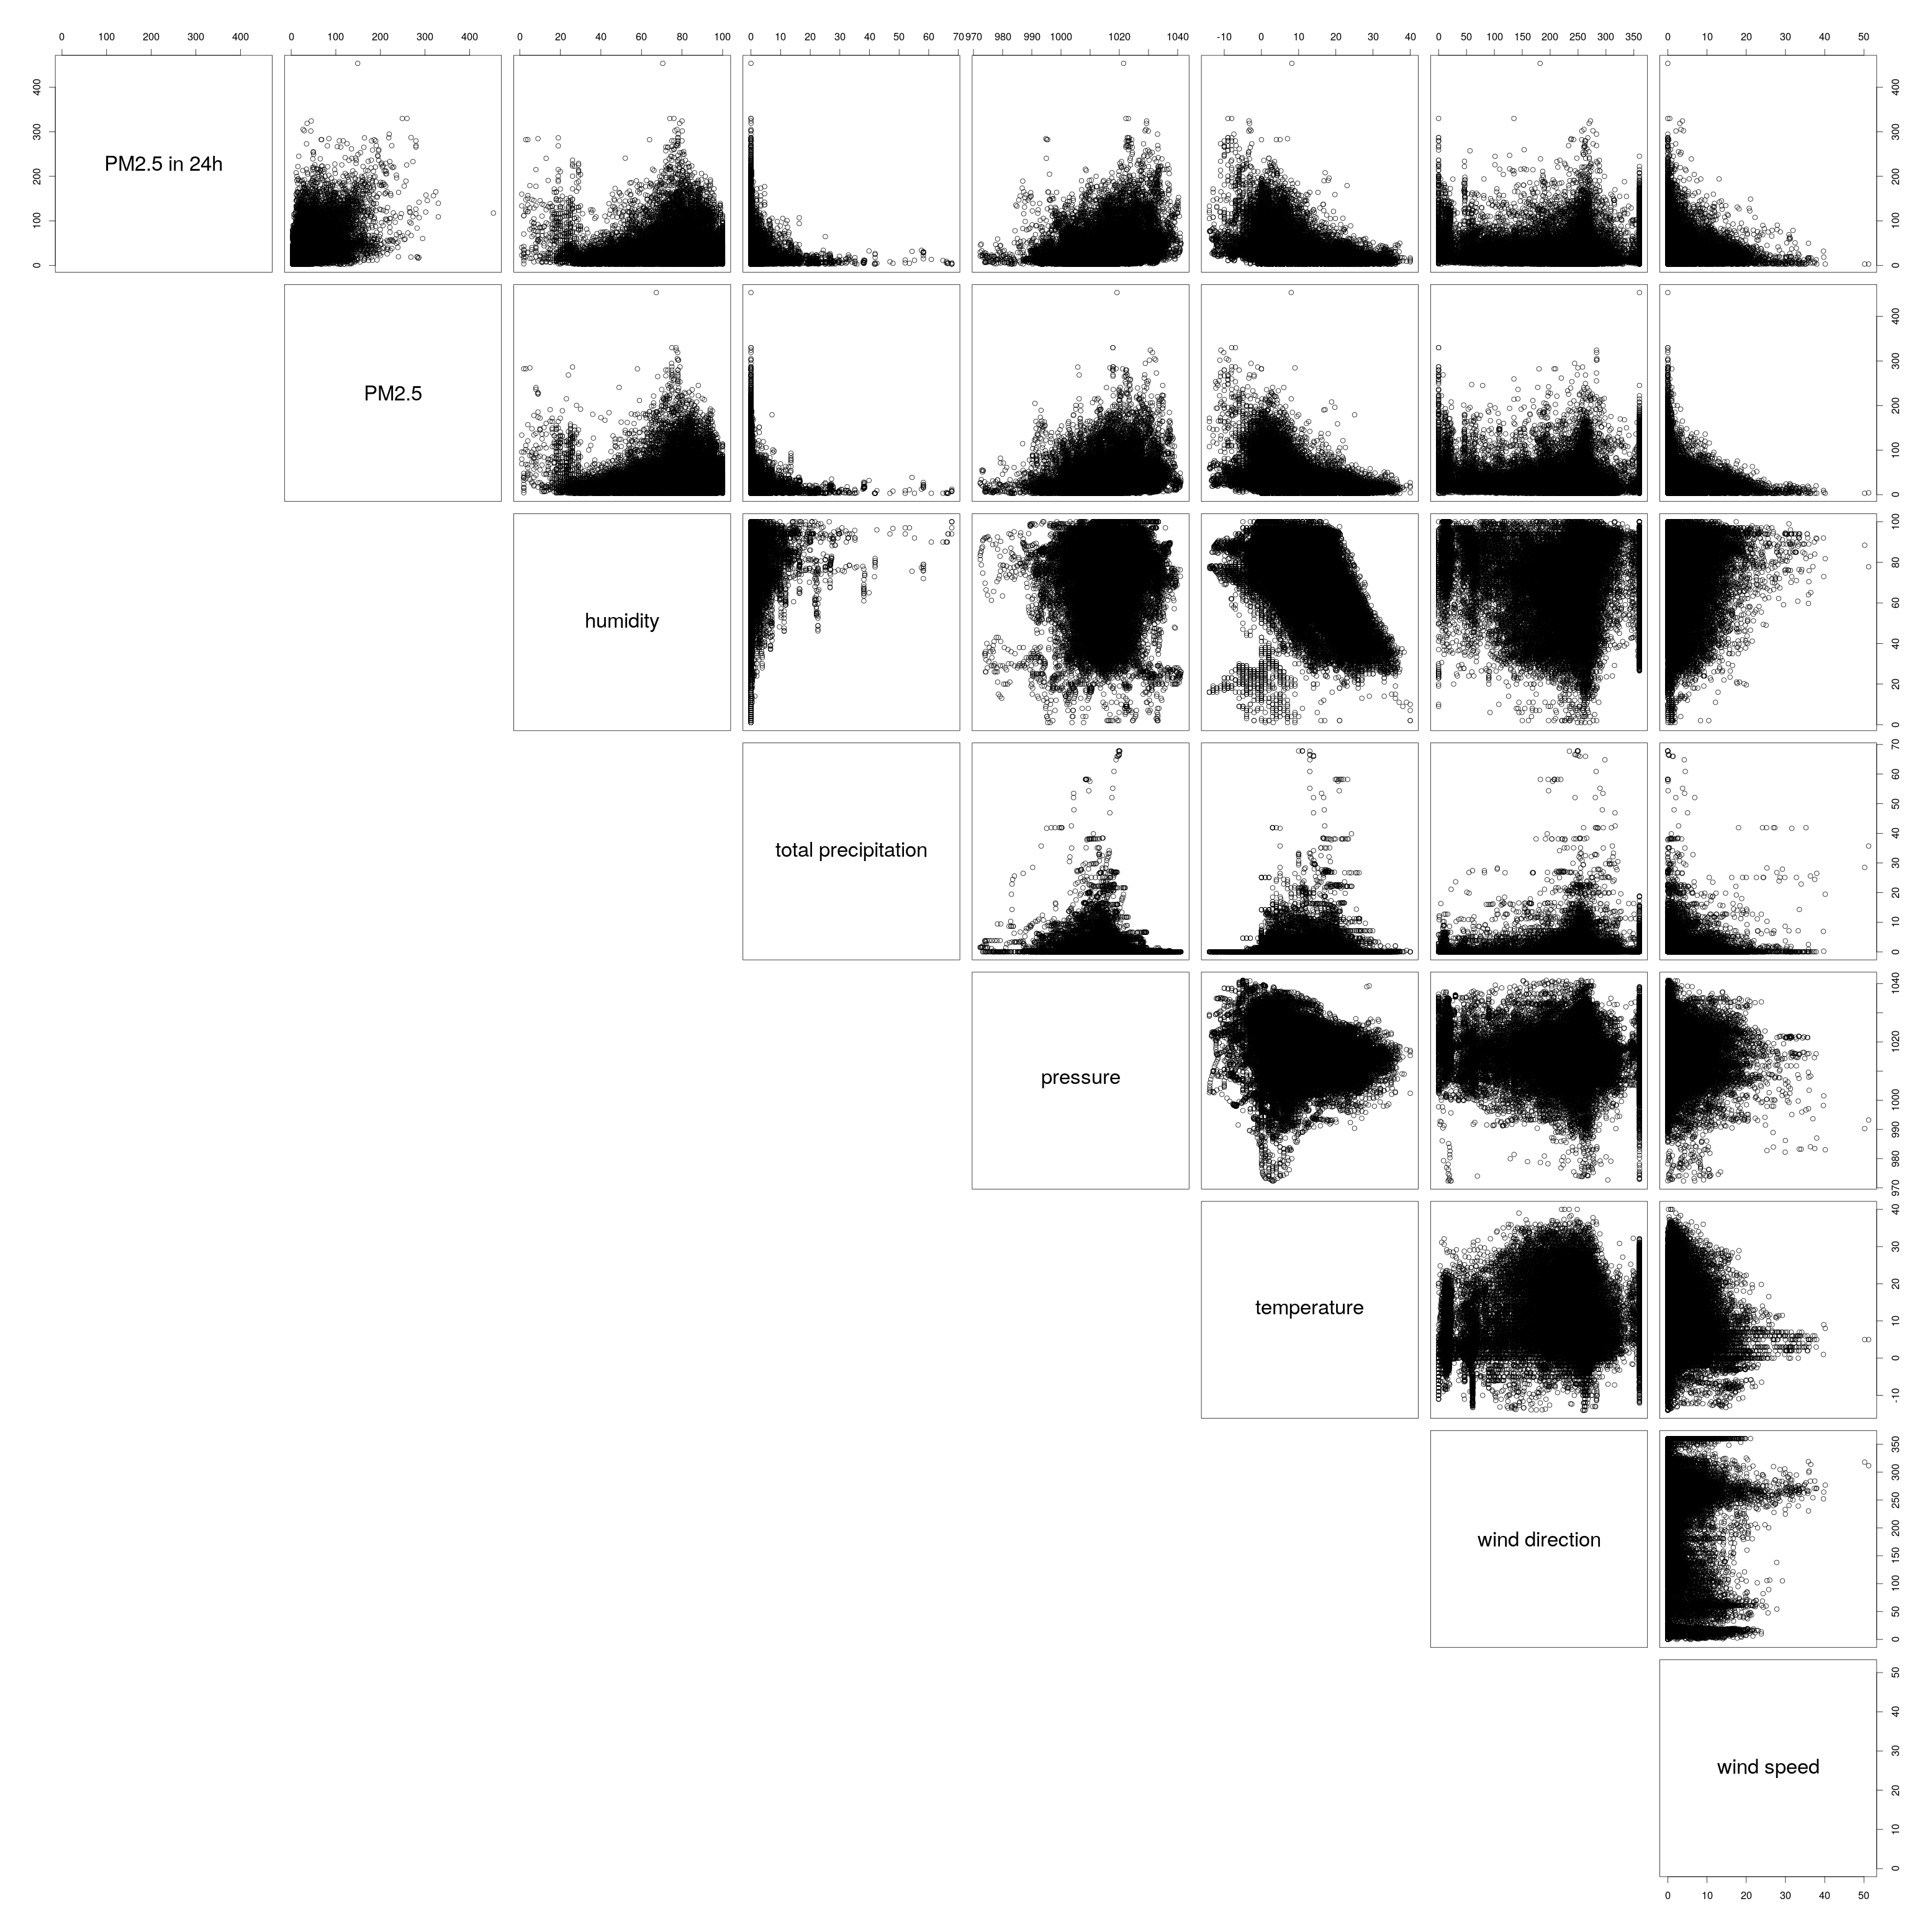
\includegraphics[width=0.65\linewidth]{figures/dataset/bivariate/relationships_gios_bulwarowa.png}
    \caption{Bivariate relationships - GIOŚ Bulwarowa}
    \label{fig:dataset-bivariate-bulwarowa}
\end{figure}
\end{landscape}
\begin{landscape}
\begin{figure}[htp]
\centering
  \centering
  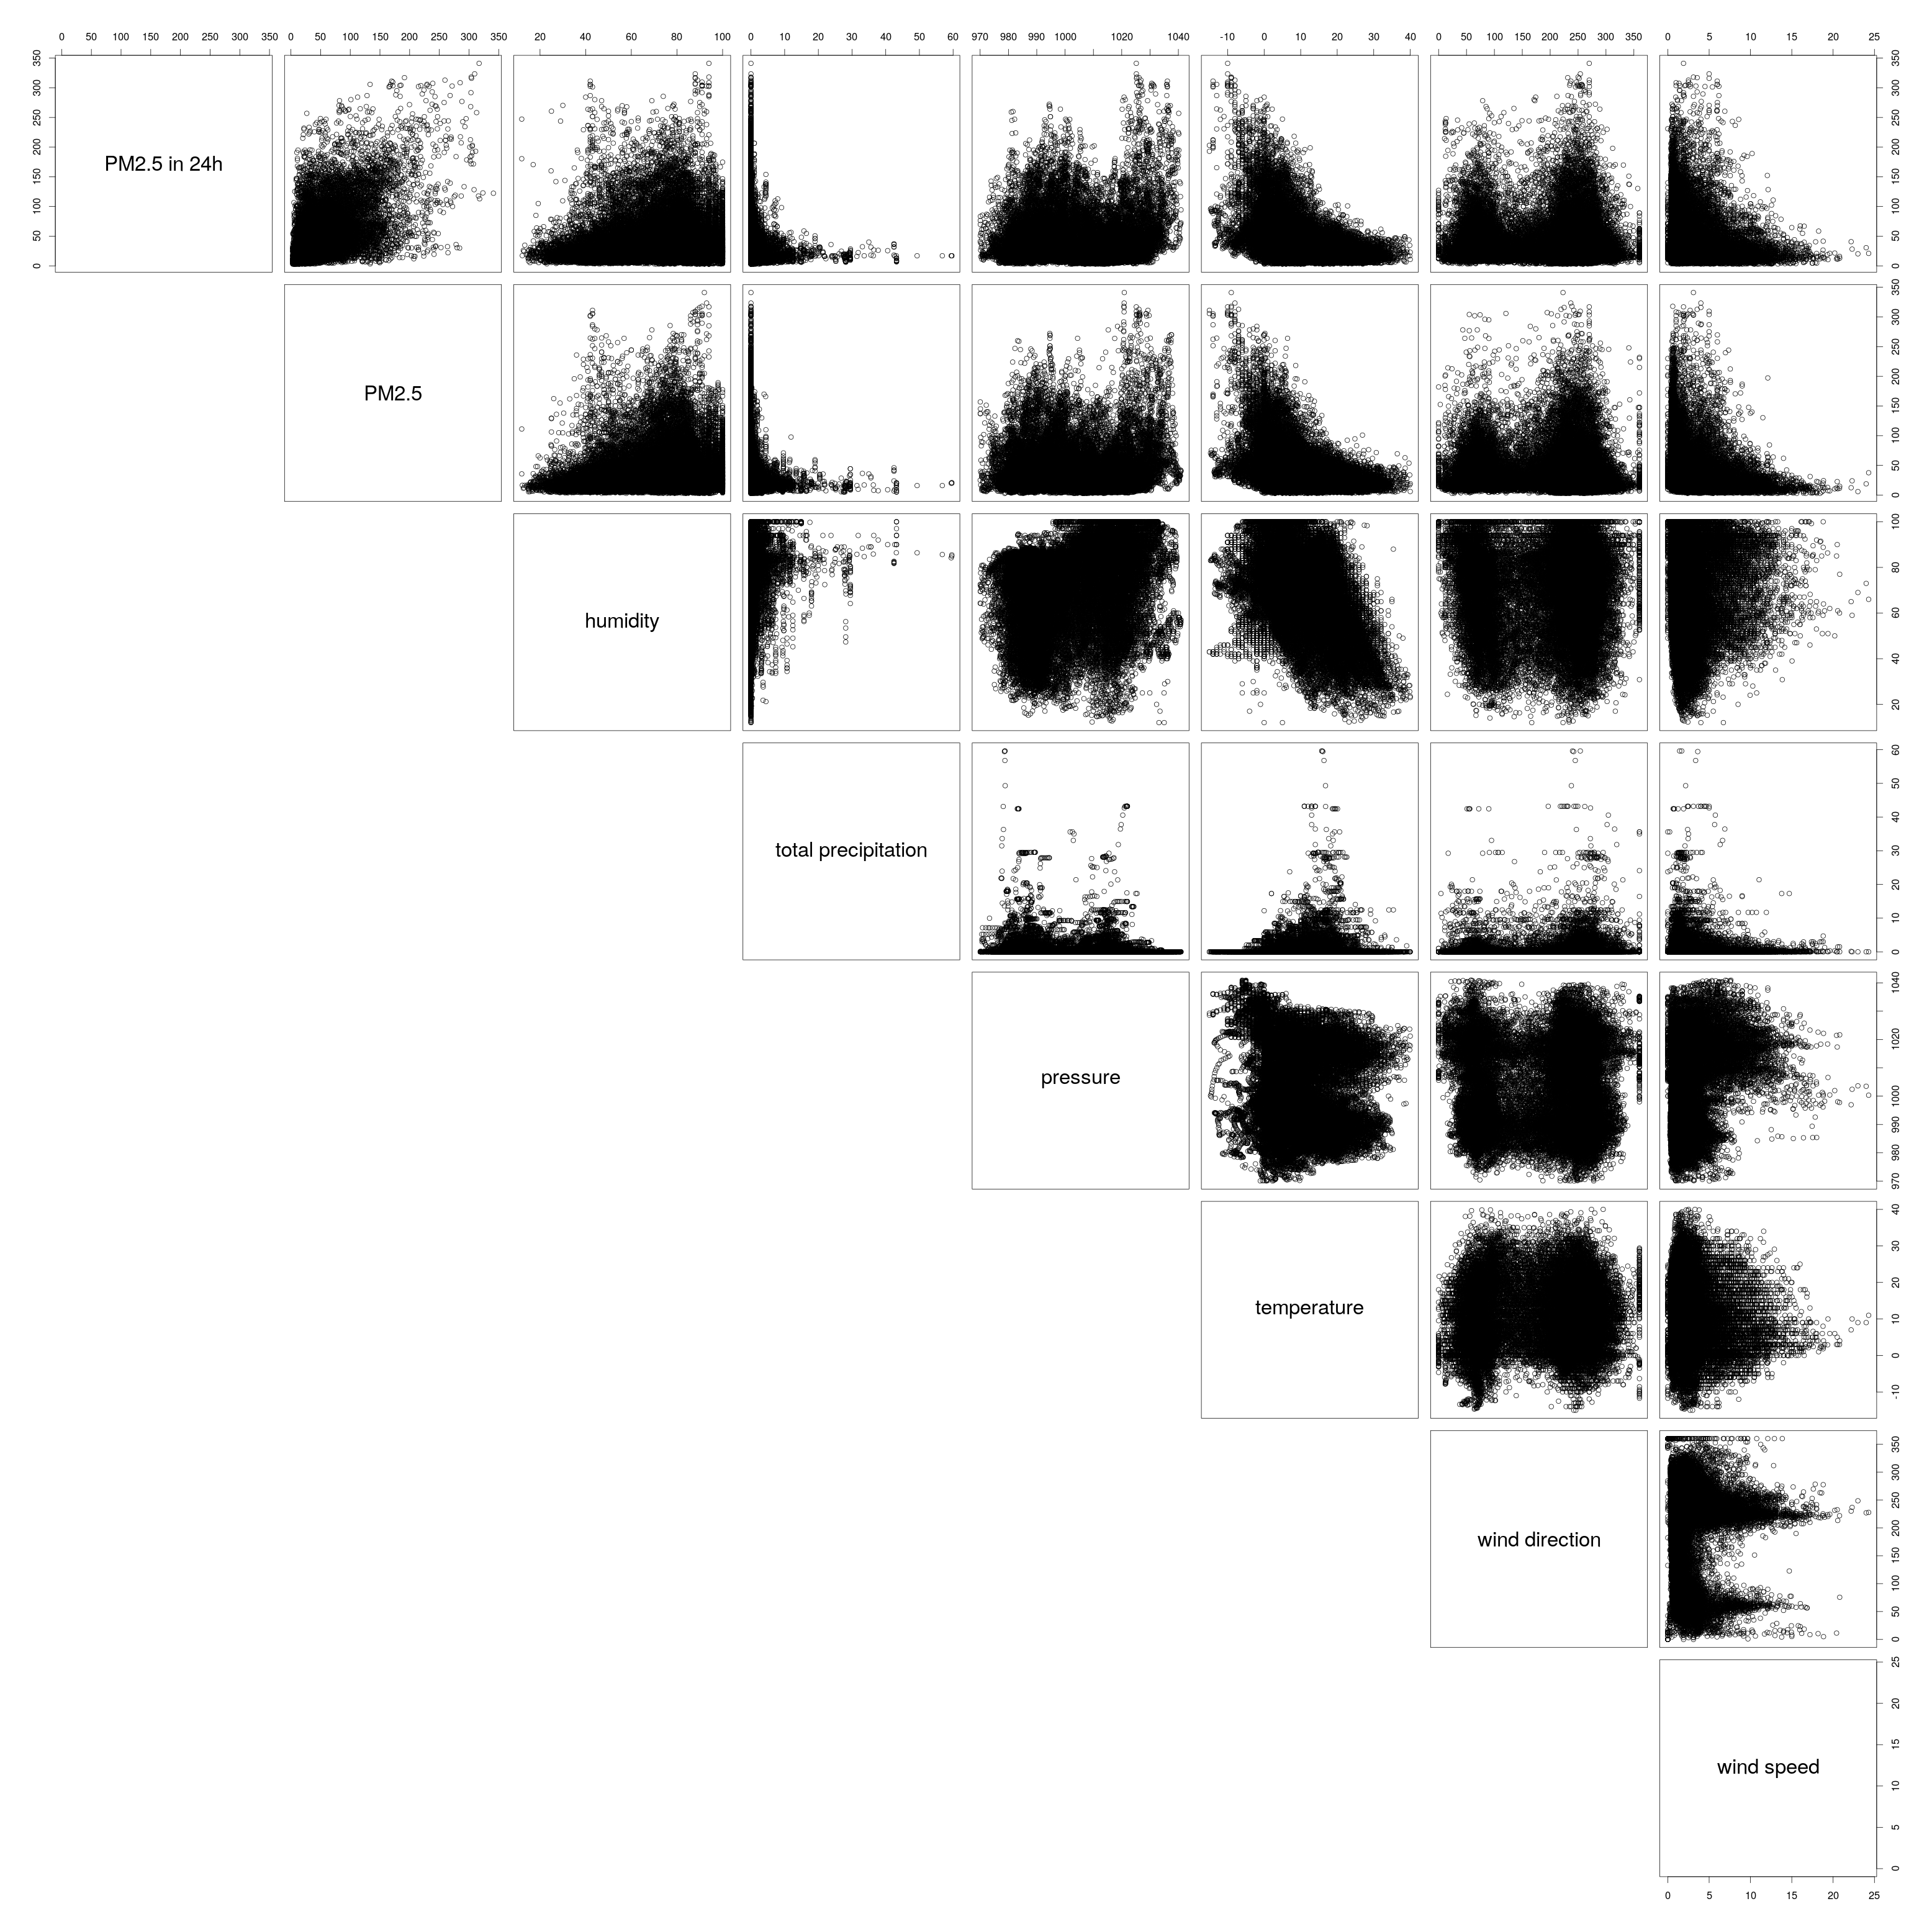
\includegraphics[width=0.65\linewidth]{figures/dataset/bivariate/relationships_gios_krasinskiego.png}
  \caption{Bivariate relationships - GIOŚ Krasińskiego}
  \label{fig:dataset-bivariate-krasinskiego}
  \end{figure}
\end{landscape}

% CORRELATION %

% \begin{figure}[htp]
% \centering
%       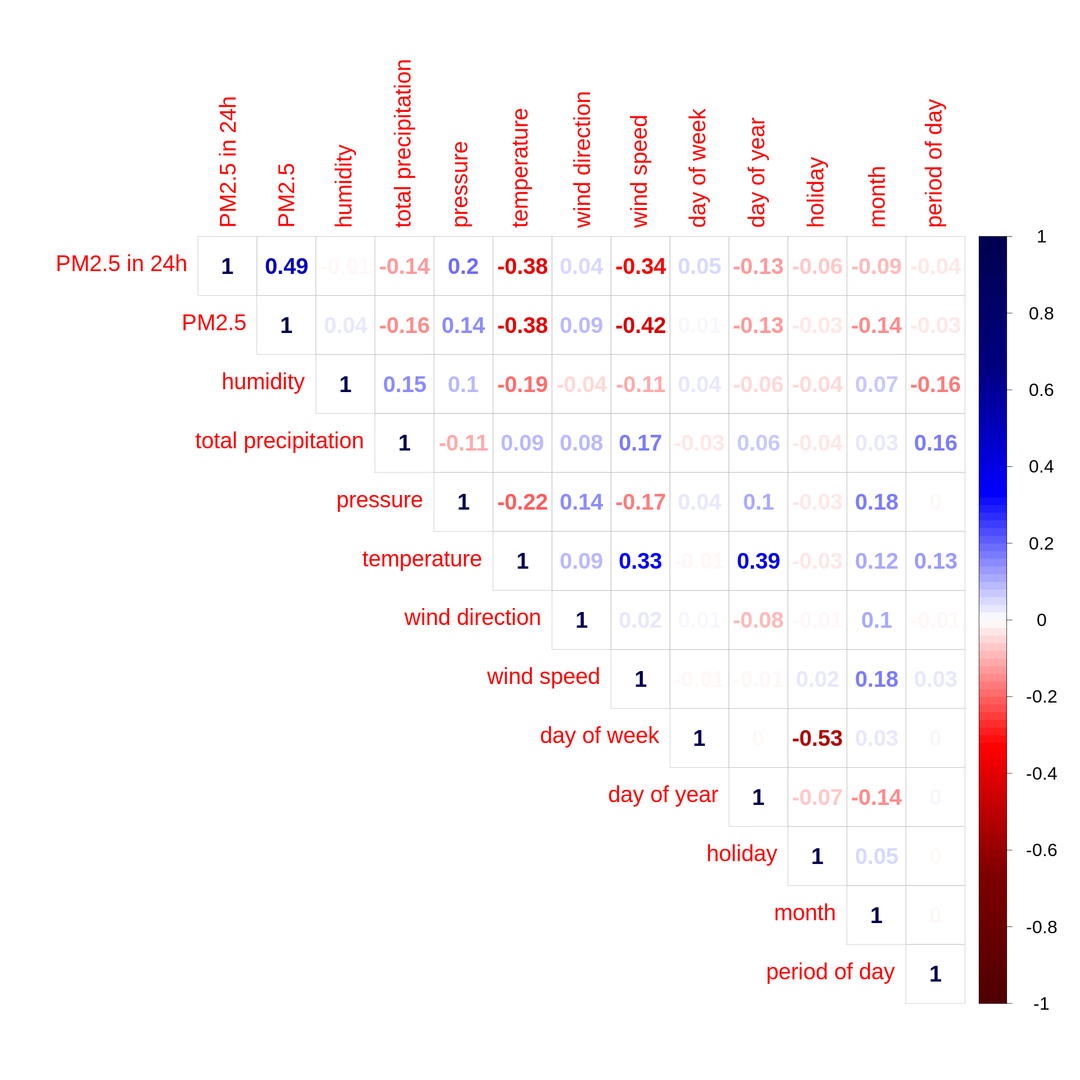
\includegraphics[width=\linewidth]{figures/dataset/correlation/corrplot_gios_bujaka_1.png}
%       \caption{Correlation plots - winter, GIOŚ Bujaka}
%       \label{fig:dataset-correlation-winter-bujaka}
% \end{figure}
% \begin{figure}[htp]
% \centering
%       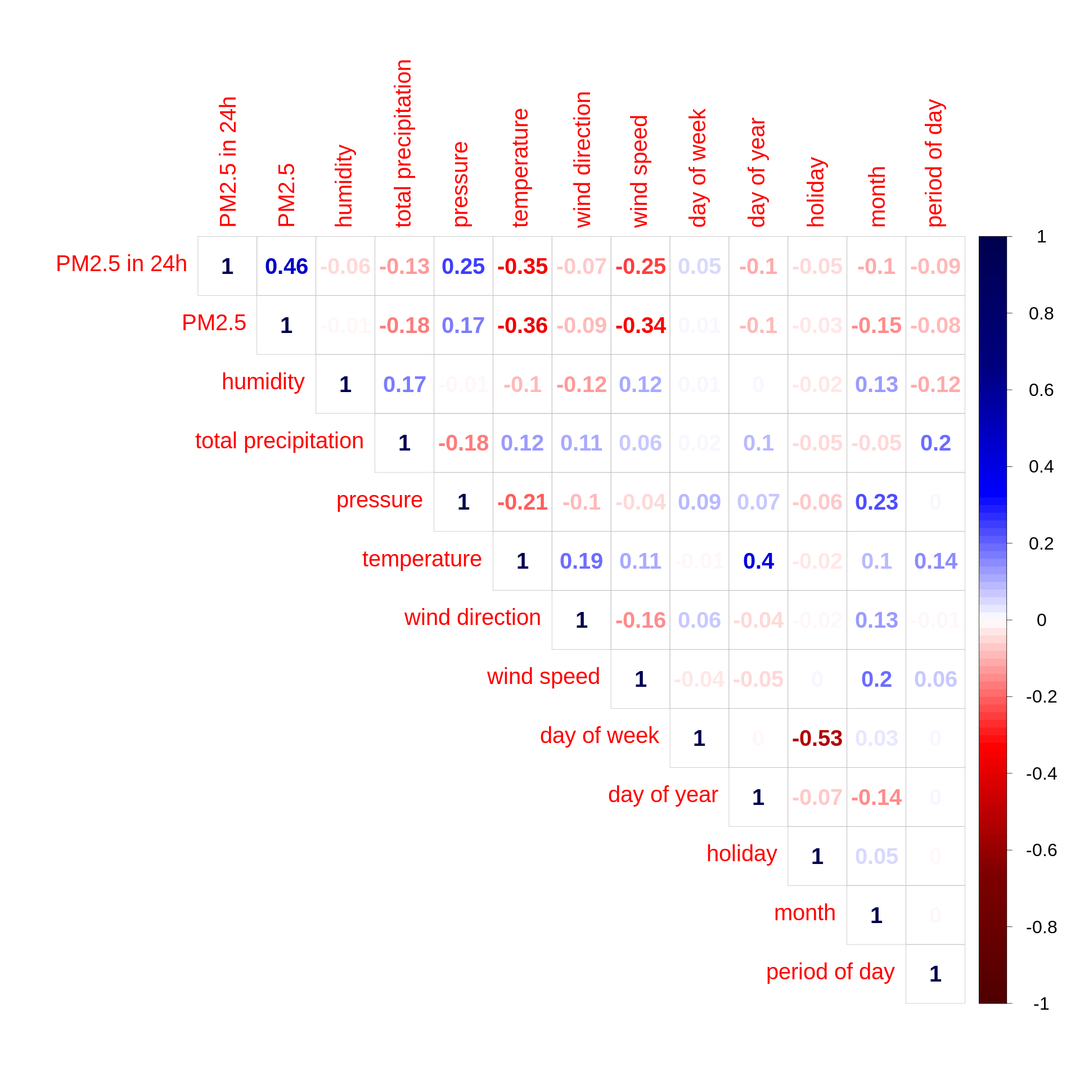
\includegraphics[width=\linewidth]{figures/dataset/correlation/corrplot_gios_bulwarowa_1.png}
%       \caption{Correlation plots - winter, GIOŚ Bulwarowa}
%       \label{fig:dataset-correlation-winter-bulwarowa}
% \end{figure}
% \begin{figure}[htp]
% \centering
%       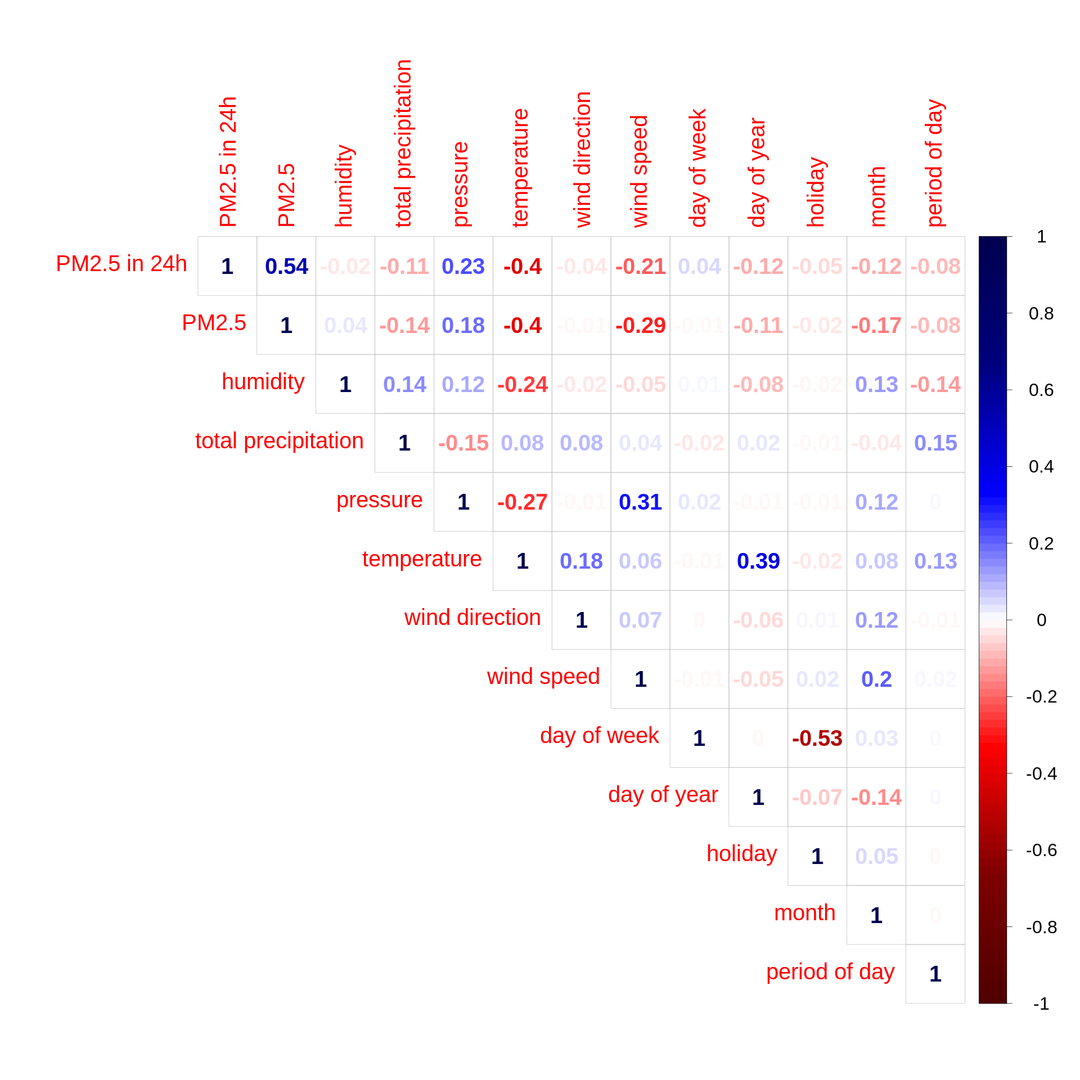
\includegraphics[width=\linewidth]{figures/dataset/correlation/corrplot_gios_krasinskiego_1.png}
%       \caption{Correlation plots - winter, GIOŚ Krasińskiego}
%       \label{fig:dataset-correlation-winter-krasinskiego}
% \end{figure}

% \begin{figure}[htp]
% \centering
%       \centering
%       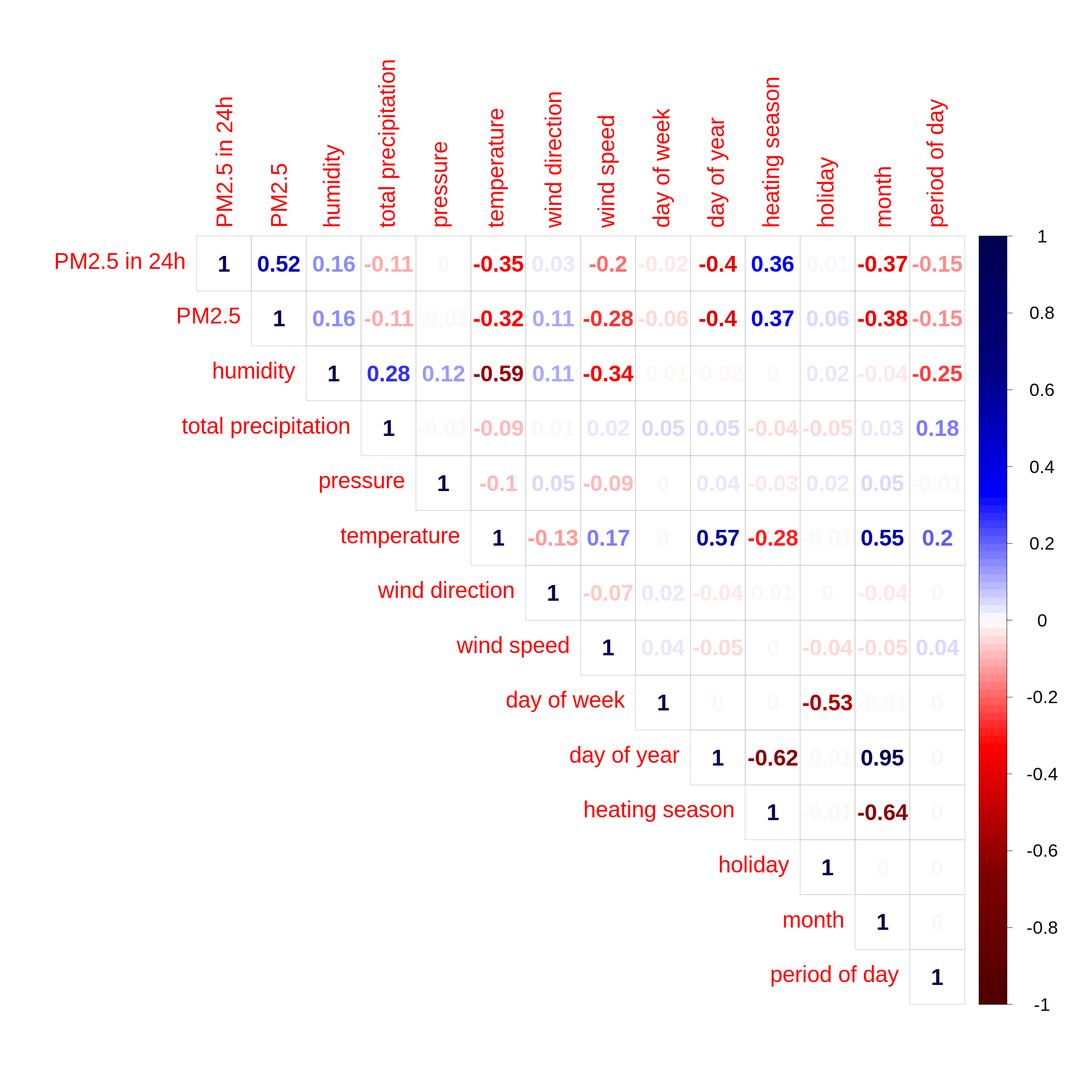
\includegraphics[width=\linewidth]{figures/dataset/correlation/corrplot_gios_bujaka_2.png}
%       \caption{Correlation plots - spring, GIOŚ Bujaka}
%       \label{fig:dataset-correlation-spring-bujaka}
% \end{figure}
% \begin{figure}[htp]
% \centering
%       \centering
%       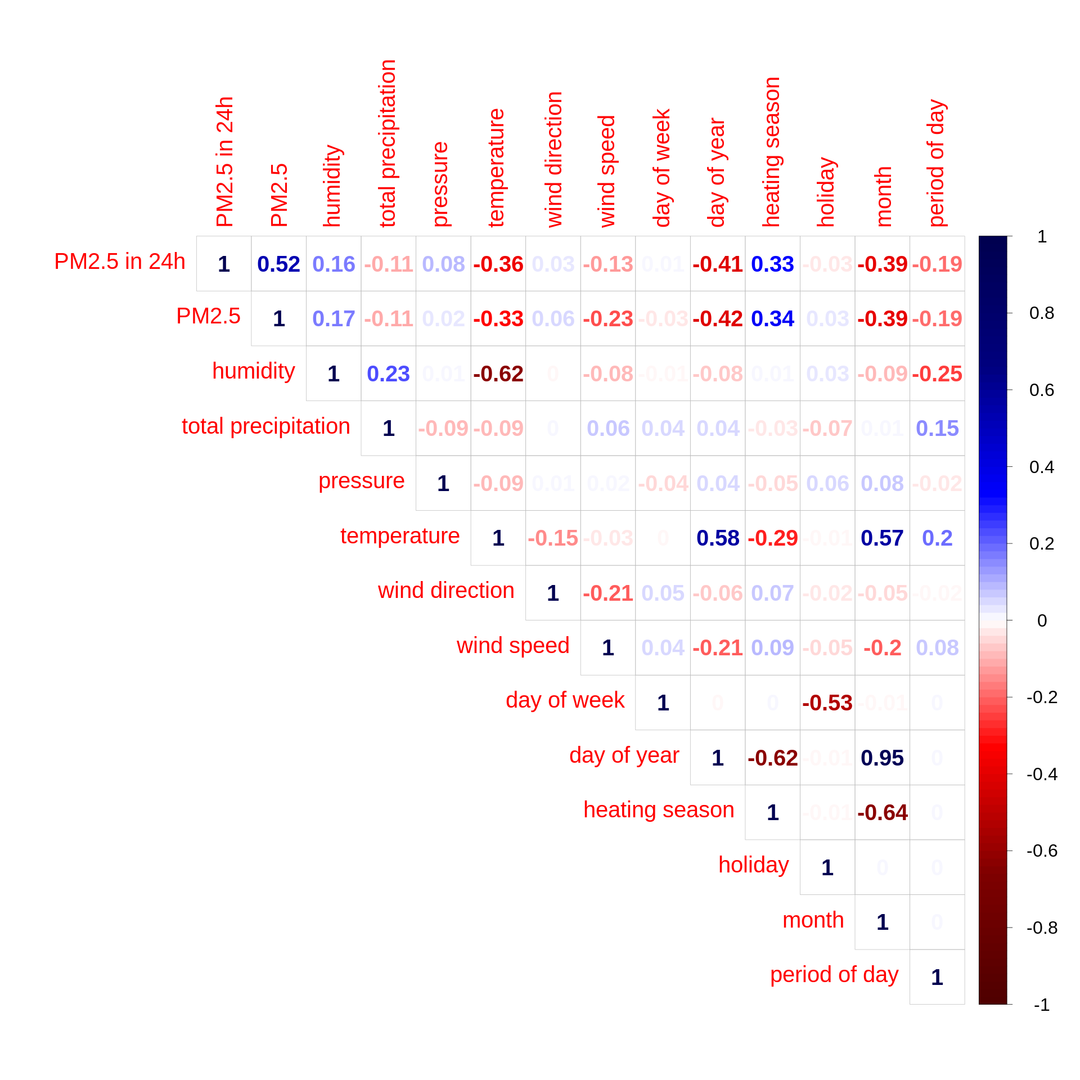
\includegraphics[width=\linewidth]{figures/dataset/correlation/corrplot_gios_bulwarowa_2.png}
%       \caption{Correlation plots - spring, GIOŚ Bulwarowa}
%       \label{fig:dataset-correlation-spring-bulwarowa}
% \end{figure}
% \begin{figure}[htp]
% \centering
%       \centering
%       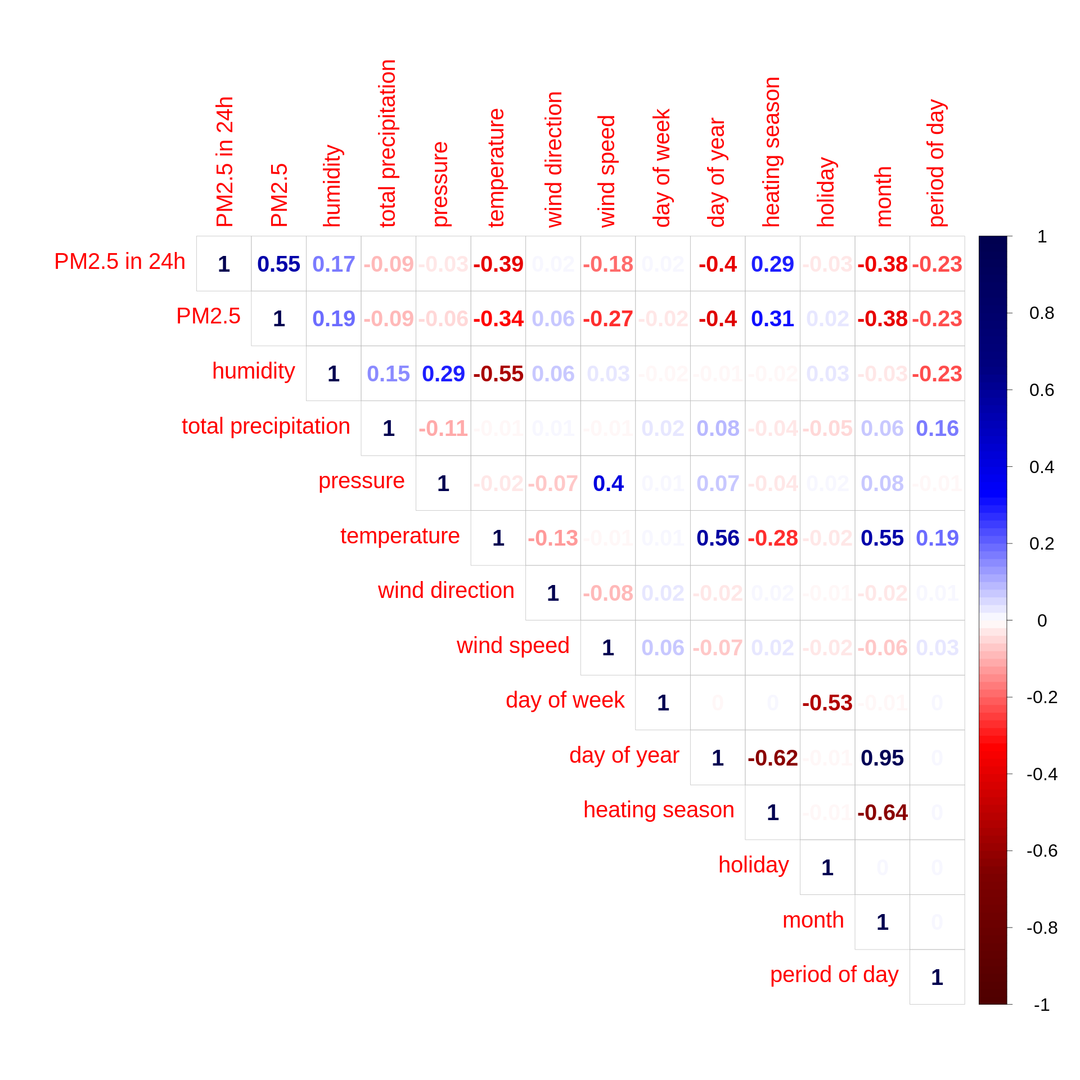
\includegraphics[width=\linewidth]{figures/dataset/correlation/corrplot_gios_krasinskiego_2.png}
%       \caption{Correlation plots - spring, GIOŚ Krasińskiego}
%       \label{fig:dataset-correlation-spring-krasinskiego}
% \end{figure}

% \begin{figure}[htp]
% \centering
%       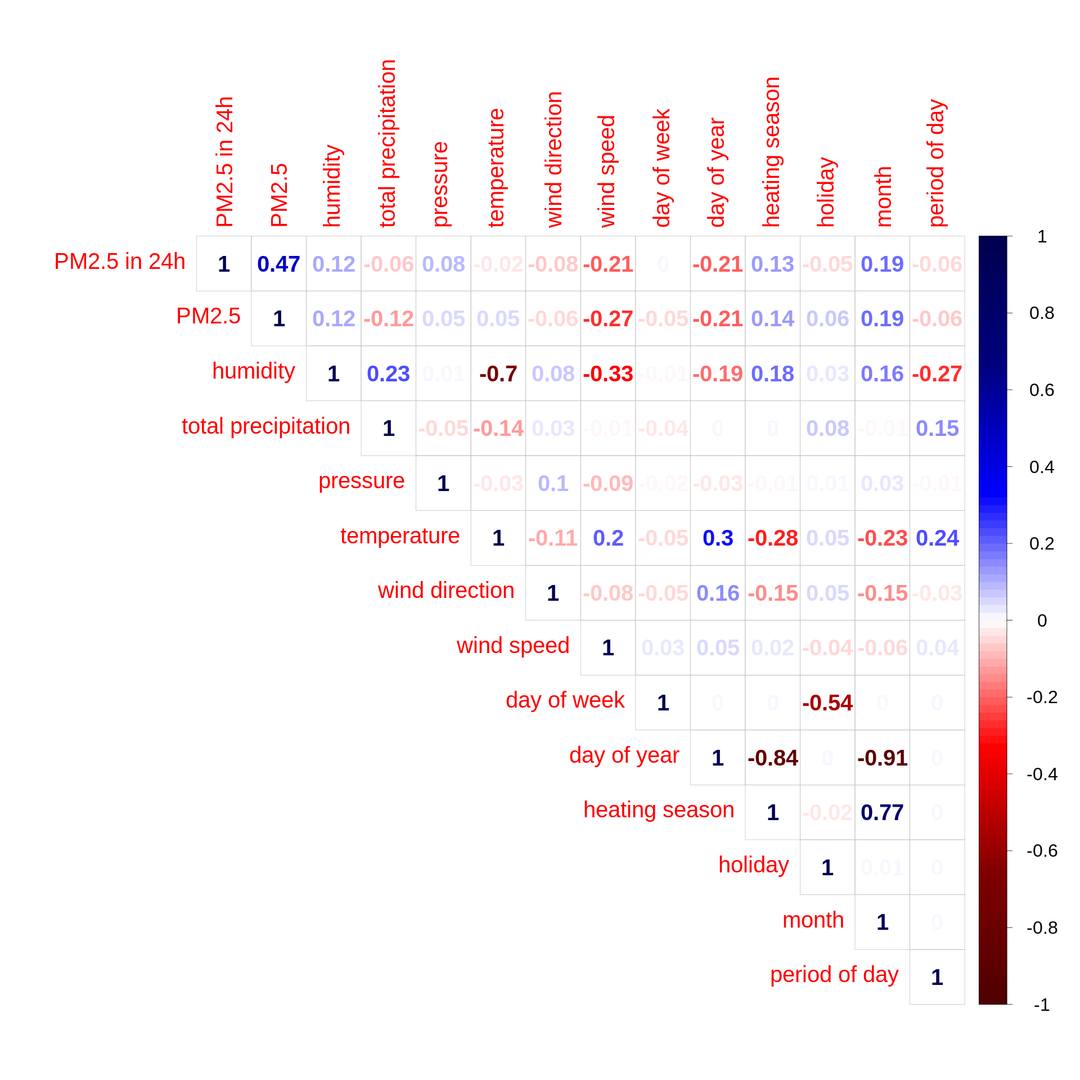
\includegraphics[width=\linewidth]{figures/dataset/correlation/corrplot_gios_bujaka_3.png}
%       \caption{Correlation plots - summer, GIOŚ Bujaka}
%       \label{fig:dataset-correlation-summer-bujaka}
% \end{figure}
% \begin{figure}[htp]
% \centering
%       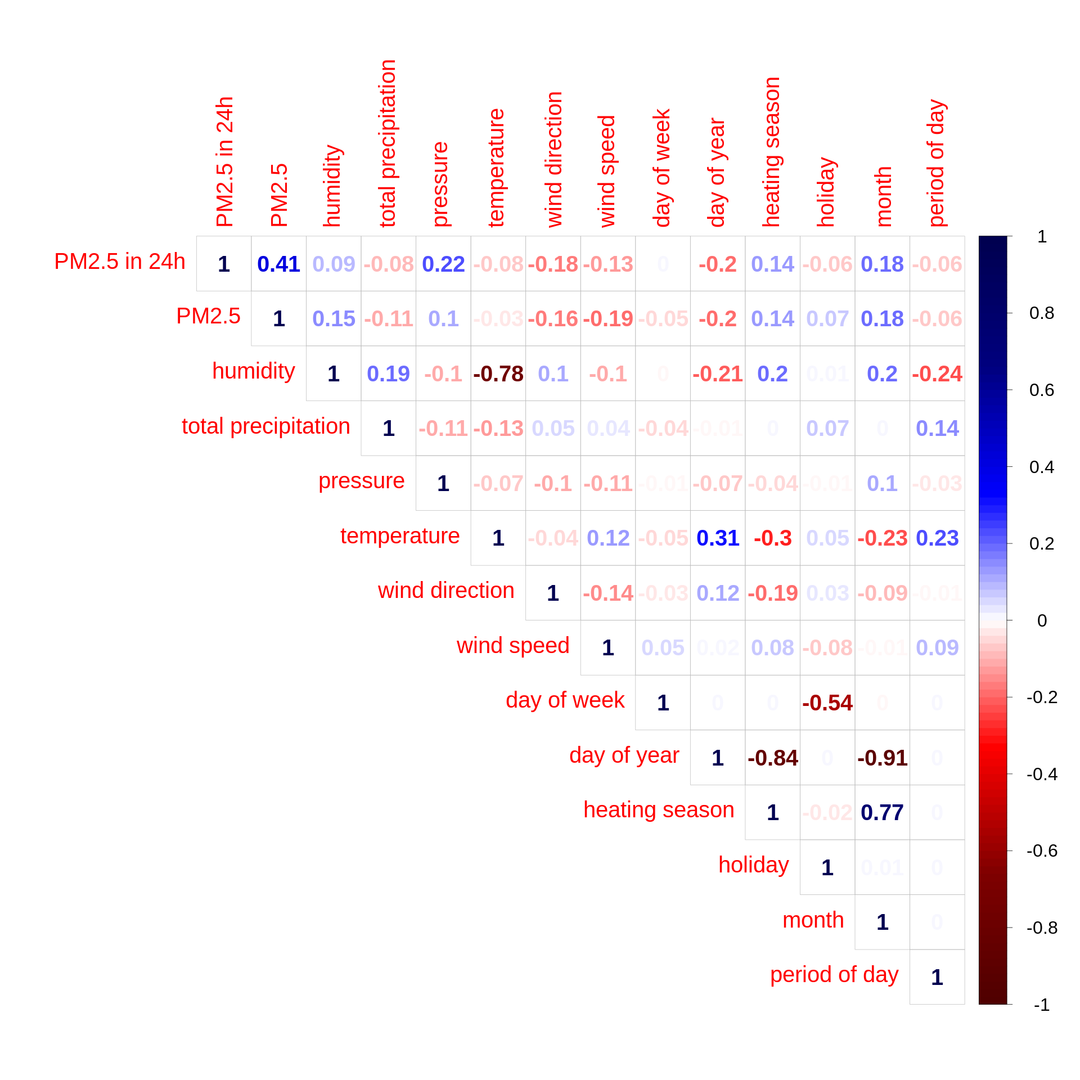
\includegraphics[width=\linewidth]{figures/dataset/correlation/corrplot_gios_bulwarowa_3.png}
%       \caption{Correlation plots - summer, GIOŚ Bulwarowa}
%       \label{fig:dataset-correlation-summer-bulwarowa}
% \end{figure}
% \begin{figure}[htp]
% \centering
%       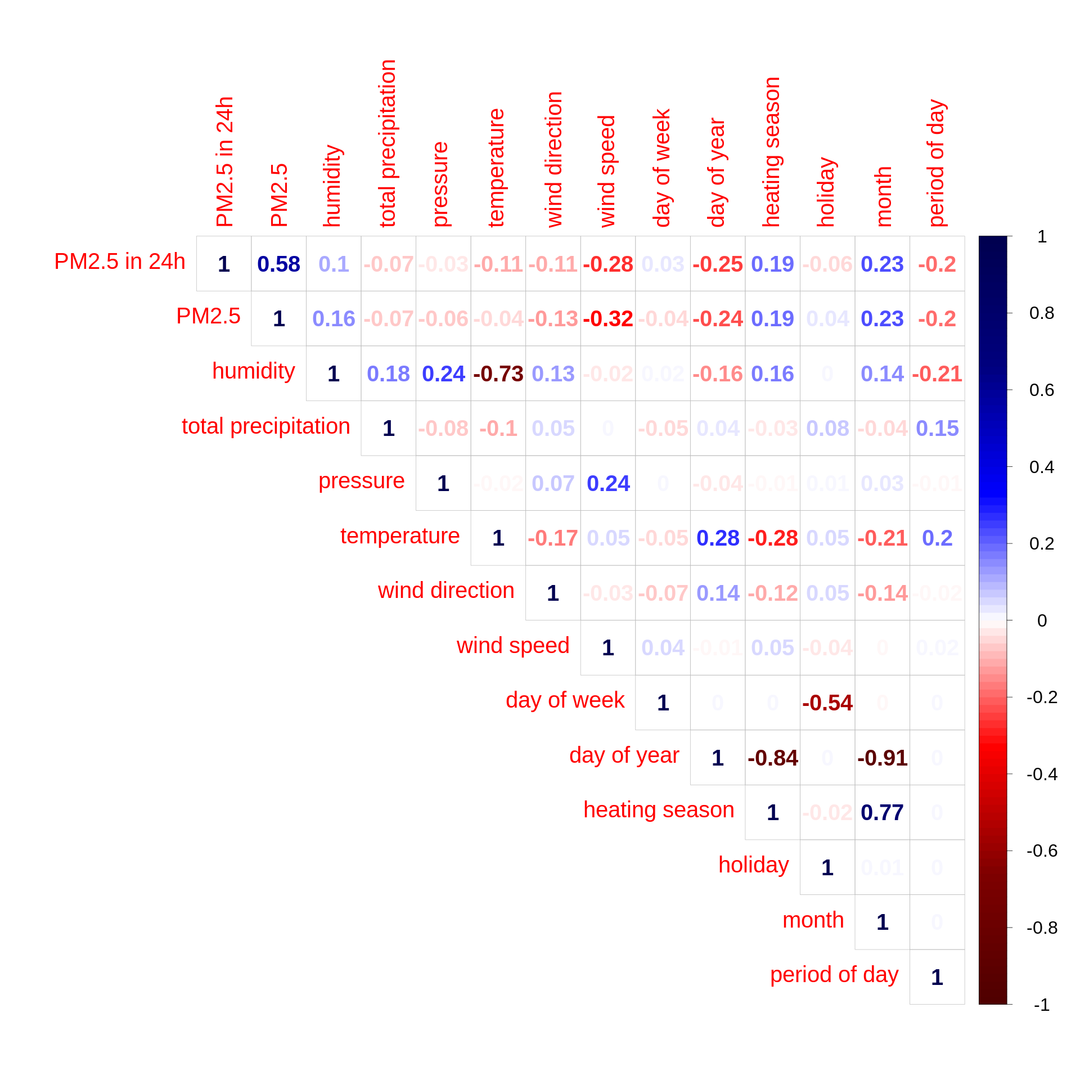
\includegraphics[width=\linewidth]{figures/dataset/correlation/corrplot_gios_krasinskiego_3.png}
%       \caption{Correlation plots - summer, GIOŚ Krasińskiego}
%       \label{fig:dataset-correlation-summer-krasinskiego}
% \end{figure}

% \begin{figure}[htp]
% \centering
%       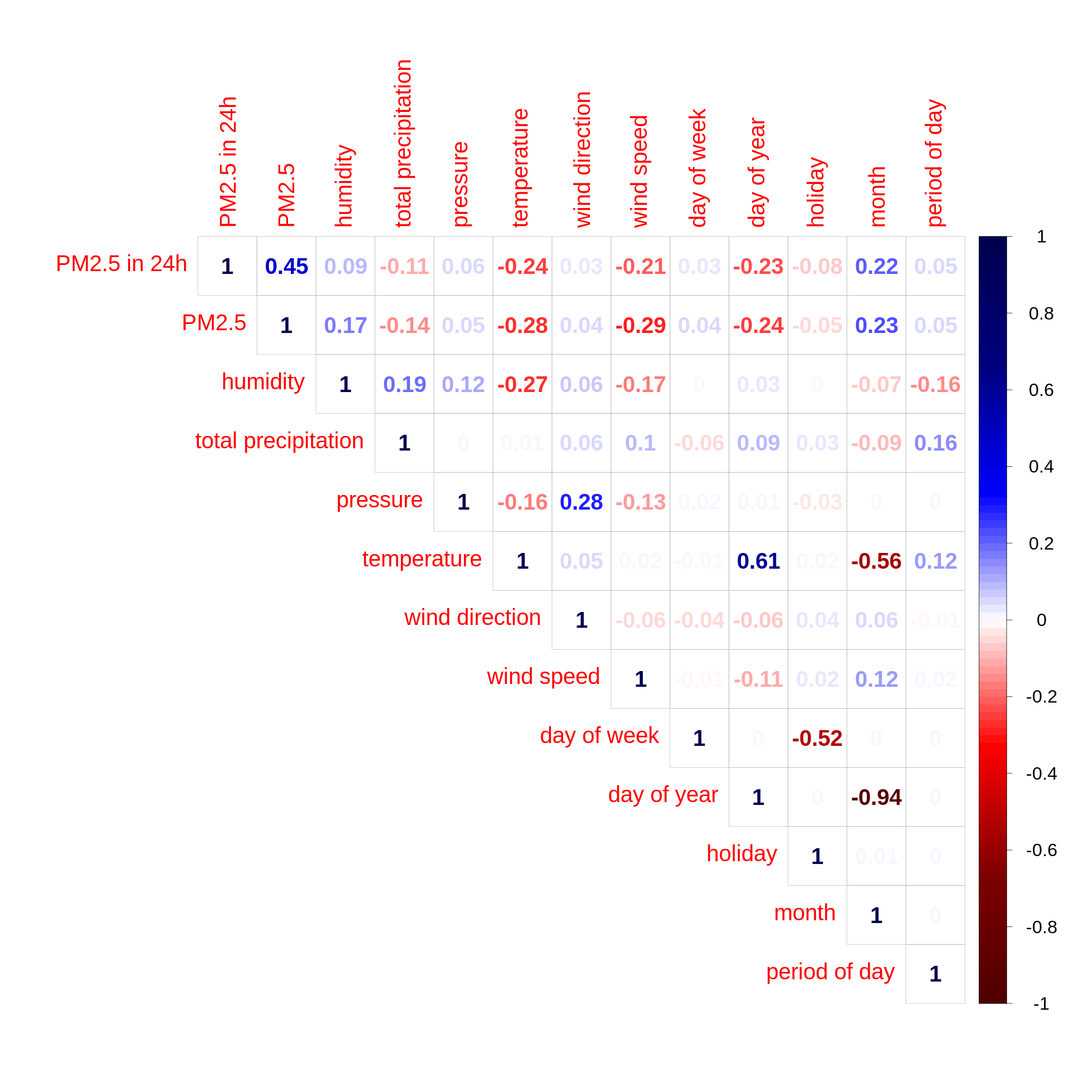
\includegraphics[width=\linewidth]{figures/dataset/correlation/corrplot_gios_bujaka_4.png}
%       \caption{Correlation plots - autumn, GIOŚ Bujaka}
%       \label{fig:dataset-correlation-autumn-bujaka}
% \end{figure}
% \begin{figure}[htp]
% \centering
%       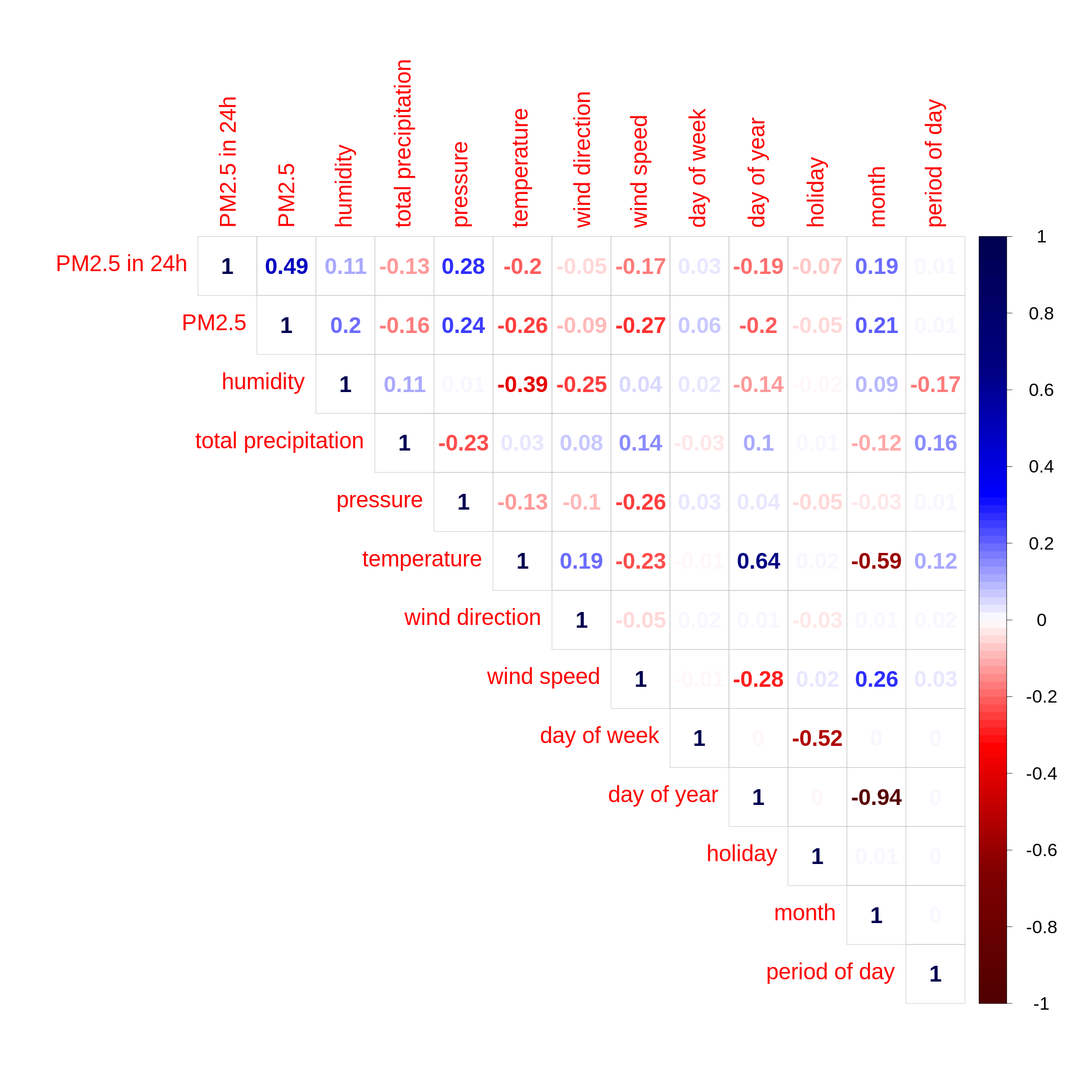
\includegraphics[width=\linewidth]{figures/dataset/correlation/corrplot_gios_bulwarowa_4.png}
%       \caption{Correlation plots - autumn, GIOŚ Bulwarowa}
%       \label{fig:dataset-correlation-autumn-bulwarowa}
% \end{figure}
% \begin{figure}[htp]
% \centering
%       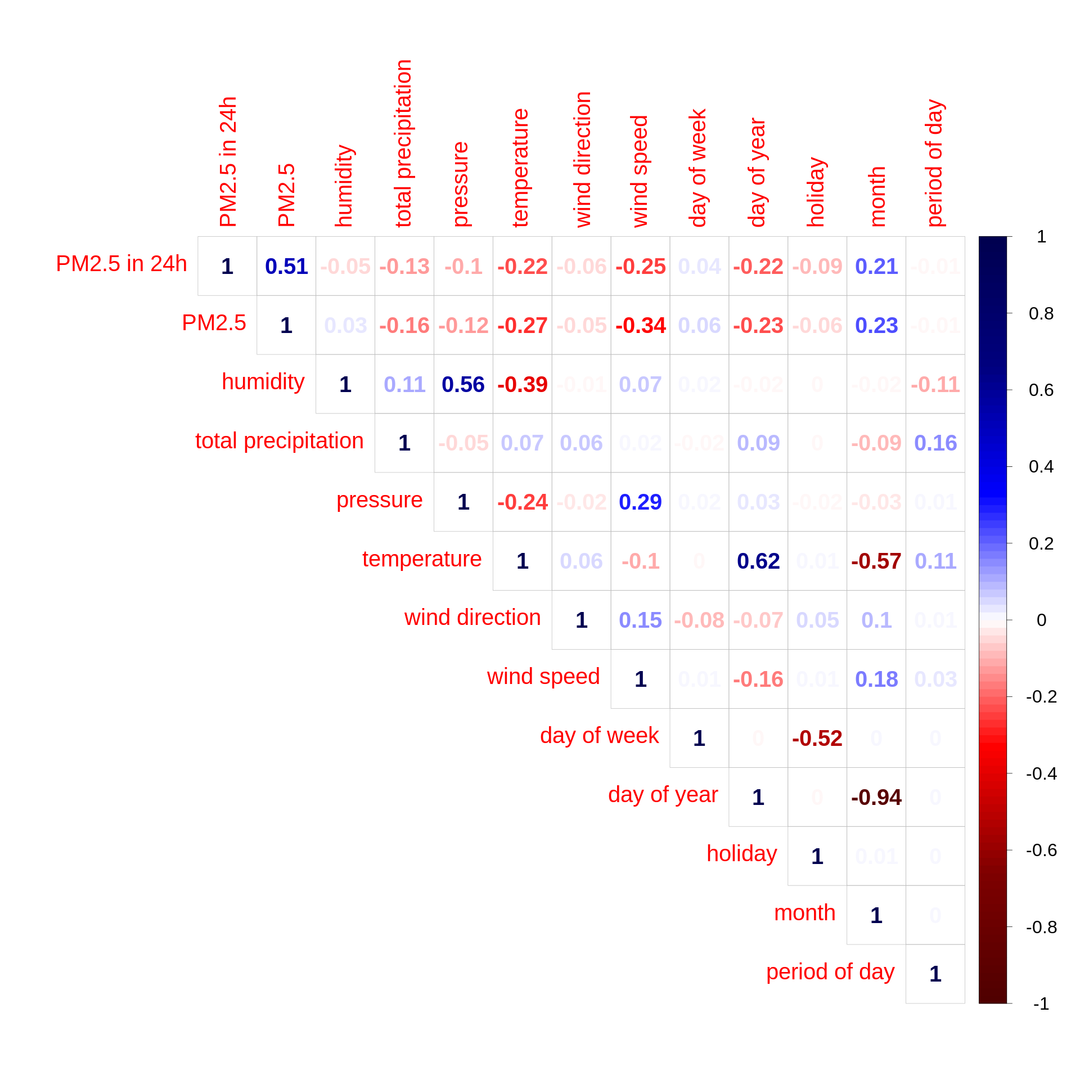
\includegraphics[width=\linewidth]{figures/dataset/correlation/corrplot_gios_krasinskiego_4.png}
%       \caption{Correlation plots - autumn, GIOŚ Krasińskiego}
%       \label{fig:dataset-correlation-autumn-krasinskiego}
% \end{figure}


\begin{landscape}
\begin{table}[H]
\centering
\footnotesize
\caption{Variables with absolute correlation to future PM2.5 concentrations greater than 0.2}
\label{tab:dataset-correlation-significant}
\begin{tabular}{llrrrrrr}
\toprule
Station & Season & \multicolumn{6}{c}{Significant variables} \\ \midrule
 &  & PM2.5 & temperature & wind speed &  &  &  \\
GIOS Bujaka & winter & 0.438 & -0.374 & -0.333 &  &  &  \\ \midrule
 &  & PM2.5 & temperature & pressure & wind speed &  &  \\
GIOS Bulwarowa & winter & 0.429 & -0.336 & 0.249 & -0.249 &  &  \\ \midrule
 &  & PM2.5 & temperature & pressure & wind speed &  &  \\
GIOS Krasinskiego & winter & 0.534 & -0.397 & 0.23 & -0.211 &  &  \\ \midrule
 &  & PM2.5 & day of year & month & heating season & temperature &  \\
GIOS Bujaka & spring & 0.512 & -0.394 & -0.365 & 0.351 & -0.349 &  \\ \midrule
 &  & PM2.5 & day of year & month & temperature & heating season &  \\
GIOS Bulwarowa & spring & 0.497 & -0.404 & -0.379 & -0.351 & 0.316 &  \\ \midrule
 &  & PM2.5 & day of year & temperature & month & heating season & period of day \\
GIOS Krasinskiego & spring & 0.542 & -0.393 & -0.376 & -0.37 & 0.282 & -0.223 \\ \midrule
 &  & PM2.5 & wind speed & day of year &  &  &  \\
GIOS Bujaka & summer & 0.462 & -0.223 & -0.219 &  &  &  \\ \midrule
 &  & PM2.5 & pressure &  &  &  &  \\
GIOS Bulwarowa & summer & 0.411 & 0.228 &  &  &  &  \\ \midrule
 &  & PM2.5 & wind speed & day of year & month &  &  \\
GIOS Krasinskiego & summer & 0.556 & -0.276 & -0.236 & 0.217 &  &  \\ \midrule
 &  & PM2.5 & temperature & day of year & month & wind speed &  \\
GIOS Bujaka & autumn & 0.446 & -0.237 & -0.223 & 0.214 & -0.204 &  \\ \bottomrule
 &  & PM2.5 & pressure & month &  &  &  \\
GIOS Bulwarowa & autumn & 0.442 & 0.257 & 0.203 &  &  &  \\ \midrule
 &  & PM2.5 & wind speed & temperature & day of year & month &  \\
GIOS Krasinskiego & autumn & 0.502 & -0.246 & -0.222 & -0.21 & 0.204 &  \\ \midrule
\end{tabular}
\end{table}
\end{landscape}
\chapter{Results}\label{chap:results}

The goodness of prediction achieved by the tested models was registered using the following measures:
\begin{itemize}

    \item Mean Absolute Error (equation \ref{eq:results-mae}),
\begin{equation}\label{eq:results-mae}
MAE = \frac{1}{n} \sum_{i = 1}^{n} |a_i - p_i|
\end{equation}

    \item Mean Absolute Percentage Error (equation \ref{eq:results-mape}),
\begin{equation}\label{eq:results-mape}
MAPE = \frac{1}{n} \sum_{i = 1}^{n} |a_i - p_i| \cdot 100\%
\end{equation}

    \item coefficient of determination $R^2$ (equation \ref{eq:results-r2}),
\begin{equation}\label{eq:results-r2}
R^2 = 1 - \frac{
    \sum_{i = 1}^{n} (a_i - p_i)^2
}{
    \sum_{i = 1}^{n} (a_i - \bar{a})^2
}
\end{equation}

    \item Root Mean Square Error (equation \ref{eq:results-rmse}).
\end{itemize}
\begin{equation}\label{eq:results-rmse}
RMSE = \sqrt{
    \frac{1}{n} \sum_{i = 1}^{n} (a_i - p_i)^2
}
\end{equation}
Symbols used in the equations \ref{eq:results-mae} - \ref{eq:results-rmse} have the following meaning: $n$ is the number of test samples, $a_i$ is the actual value of the $i^{th}$ sample, $p_i$ is the $i^{th}$ predicted value and $\bar{a}$ is the mean value of actual PM2.5 concentrations.
\\\\
% Results of the experiments can be found in tables \ref{tab:results-bujaka-all-data} - \ref{tab:results-krasinskiego-same-season}. In order to make them easier to interpret they are also presented in the form of figures
Results of the experiments are presented in figures \ref{fig:results-best-bujaka-all-data} - \ref{fig:results-best-krasinskiego-same-season}. Scores for the neural networks were averaged based on 5 repetitions of the testing procedure in order to deal with the consequences of the random weight initialisation.
% \\\\
% Figures \ref{fig:results-comparison-bujaka-winter-all-data} - \ref{fig:results-comparison-krasinskiego-autumn-same-season} contain comparisons of the actual and predicted PM2.5 concentrations for the best models. Their statistics are grouped in table 
A summary of the best results can be found in table \ref{tab:results-best-models}. The ranking was prepared with the Root Mean Square Error as the main score. The errors vary for different seasons. In winter they range from 43.912 to 55.634 $\mu g/m^3$, in spring - from 14.408 to 16.306 $\mu g/m^3$, in summer from 6.855 to 8.856 and in autumn from 21.768 to 25.870 $\mu g/m^3$. The magnitude of errors seems to be connected with the magnitude of PM2.5 concentrations during a specific season and at a particular spot - the highest errors occurred in winter, while the lowest in summer. Additionally, in most cases, the highest errors were noticed for the station at the Krasińskiego Avenue where the highest average PM2.5 concentrations were registered (table \ref{tab:dataset-stats-krasinskiego}). On the other hand, the training strategy does not seem to have a major impact on the accuracy - the errors tend to be similar for both methods. An interesting observation is the fact that for a particular season the same types of models tend to perform best: multiple linear regression for winter, support vector regression and neural networks for spring and summer. For autumn the best models are more varied than for the rest of the seasons. Somewhat surprising is the fact that in the case of winter SVR and neural networks were outperformed by regression, whose modelling capabilities are restricted to linear relationships.
\\\\
It is hard to tell for certain whether reusing the best found parameter values of the SVR and neural networks impacted the results for the Bujaka and Bulwarowa stations in a negative way. Models trained on the data gathered in those locations tend to score lower $R^2$ values than those for the the Krasinskiego station, however the differences concern also the non-parametric regression methods. It is possible that they stem simply from the differences between the data sets which influence the quality of predictors. 
\\\\
Overall, the performance of the investigated models might be considered reasonable, however some undesirable effects can be noticed (for example in figure \ref{fig:results-comparison-krasinskiego-winter-all-data}). The models tend to have problems with forecasting spikes of the PM2.5 levels. They are capable of indicating direction of change, however the exact concentrations are often considerably lower than the actual ones. The second problem is the fact that the predicted concentrations seem to be lagged relative to the changes taking place. If the pollutant levels are rising or falling, they are reflected by the predictions only after some delay, which reduces the usefulness of forecasting models.
\\\\
Comparing the results of the performed experiments with the findings reported in related work is problematic because of the dependence of the forecasting task on the local climate and the specific prediction goal. There have been at least two similar studies conducted for Krakow: \cite{LOZOWICKA2005} and \cite{Pawul2016}, however both of them were focused on daily means of pollutant concentrations as opposed to their hourly levels. The results of the mentioned studies can be found in table \ref{tab:related-work-results}.

\begin{landscape}
\begin{table}[ht]
\centering
\caption{Results of the best models per season, station and training strategy}
\label{tab:results-best-models}
\footnotesize
\begin{tabular}{llllrrrr}

\toprule
Model & Season & Training type & Station & RMSE [$\mu g/m^3$] & MAE [$\mu g/m^3$] & MAPE [$\%$] & $R^2$ [$1$] \\ \midrule
MLR & winter & all data & GIOŚ Bujaka & 55.634 & 38.165 & 121.460 & 0.330 \\
MLR & winter & same season & GIOŚ Bujaka & 55.349 & 41.592 & 158.581 & 0.333 \\
MLR & winter & all data & GIOŚ Bulwarowa & 43.912 & 32.168 & 117.894 & 0.334 \\
MLR LASSO & winter & same season & GIOŚ Bulwarowa & 45.958 & 35.550 & 143.292 & 0.266 \\
MLR & winter & all data & GIOŚ Krasińskiego & 51.676 & 36.081 & 78.782 & 0.429 \\
MLR & winter & same season & GIOŚ Krasińskiego & 52.197 & 37.871 & 91.895 & 0.416 \\
\midrule
ANN (6, 5), threshold = 0.7 & spring & all data & GIOŚ Bujaka & 15.585 & 9.909 & 67.350 & 0.131 \\
SVR $\gamma$ = $2^{-10}$, $\epsilon$ = 0.25, C = 0.25 & spring & same season & GIOŚ Bujaka & 15.388 & 9.832 & 65.815 & 0.154 \\
ANN (6. 5), threshold = 0.7 & spring & all data & GIOŚ Bulwarowa & 14.875 & 10.461 & 89.299 & 0.134 \\
SVR $\gamma$ = $2^{-10}$, $\epsilon$ = 0.25, C = 0.25 & spring & same season & GIOŚ Bulwarowa & 14.408 & 9.870 & 78.377 & 0.189 \\
SVR $\gamma$ = $2^{-10}$, $\epsilon$ = 2, C = 1 & spring & all data & GIOŚ Krasińskiego & 16.306 & 11.209 & 55.841 & 0.167 \\
SVR $\gamma$ = $2^{-10}$, $\epsilon$ = 0.25, C = 0.25 & spring & same season & GIOŚ Krasińskiego & 16.072 & 11.326 & 60.077 & 0.191 \\
\midrule
MLR ln(PM2.5) & summer & all data & GIOŚ Bujaka & 6.855 & 5.242 & 66.407 & 0.138 \\
SVR $\gamma$ = $2^{-12}$, $\epsilon$ = 0.5, C = 0.25 & summer & same season & GIOŚ Bujaka & 6.870 & 5.334 & 70.300 & 0.134 \\
SVR $\gamma$ = $2^{-8}$, $\epsilon$ = $2^{-5}$, C = 0.25 & summer & all data & GIOŚ Bulwarowa & 7.765 & 5.723 & 71.145 & 0.099 \\
SVR $\gamma$ = $2^{-12}$, $\epsilon$ = 0.5, C = 0.25 & summer & same season & GIOŚ Bulwarowa & 7.777 & 5.768 & 71.923 & 0.097 \\
SVR $\gamma$ = $2^{-8}$, $\epsilon$ = $2^{-5}$, C = 0.25 & summer & all data & GIOŚ Krasińskiego & 8.856 & 6.850 & 48.531 & 0.151 \\
MLR LASSO & summer & same season & GIOŚ Krasińskiego & 8.575 & 6.645 & 51.192 & 0.203 \\
\midrule
ANN (5, 5), threshold = 0.5 & autumn & all data & GIOŚ Bujaka & 21.978 & 15.857 & 103.397 & 0.177 \\
SVR $\gamma$ = $2^{-12}$, $\epsilon$ = 0.5, C = 16 & autumn & same season & GIOŚ Bujaka & 22.055 & 15.733 & 97.139 & 0.171 \\
MLR & autumn & all data & GIOŚ Bulwarowa & 21.768 & 15.579 & 104.767 & 0.204 \\
MLR LASSO & autumn & same season & GIOŚ Bulwarowa & 22.074 & 15.951 & 107.828 & 0.179 \\
ANN (5, 5), threshold = 0.5 & autumn & all data & GIOŚ Krasińskiego & 25.743 & 18.756 & 70.534 & 0.225 \\
ANN (3, 2), threshold = 0.3 & autumn & same season & GIOŚ Krasińskiego & 25.870 & 18.889 & 73.834 & 0.213 \\ \bottomrule
\end{tabular}
\end{table}
\end{landscape}

% \begin{landscape}
% \begin{table}[ht]
% \centering
% \caption{Results summary - GIOŚ Bujaka (all data)}
% \label{tab:results-bujaka-all-data}
% \begin{tabular}{llrrrr}

% \toprule
% Model & Season & RMSE [$\mu g/m^3$] & MAE [$\mu g/m^3$] & MAPE [$\%$] & R2 [$1$] \\ \midrule
% MLR & winter & 55.634 & 38.165 & 121.460 & 0.330 \\
% MLR LASSO & winter & 56.320 & 38.444 & 123.677 & 0.313 \\
% MLR ln(PM2.5) & winter & 62.273 & 37.527 & 96.082 & 0.160 \\
% ANN (5), threshold = 0.7 & winter & 66.868 & 41.796 & 112.420 & 0.018 \\
% SVR $\gamma$ = $2^{-12}$, $\epsilon$ = 0.5, C = 1 & winter & 59.322 & 36.692 & 87.726 & 0.238 \\
% \midrule MLR & spring & 17.594 & 13.034 & 101.182 & -0.107 \\
% MLR LASSO & spring & 17.128 & 12.654 & 105.250 & -0.049 \\
% MLR ln(PM2.5) & spring & 15.915 & 9.895 & 58.563 & 0.094 \\
% ANN (6, 5), threshold = 0.7 & spring & 15.585 & 9.909 & 67.350 & 0.131 \\
% SVR $\gamma$ = $2^{-10}$, $\epsilon$ = 2, C = 1 & spring & 16.110 & 10.201 & 61.312 & 0.072 \\
% \midrule MLR & summer & 11.114 & 8.707 & 112.959 & -1.265 \\
% MLR LASSO & summer & 9.048 & 7.157 & 94.609 & -0.501 \\
% MLR ln(PM2.5) & summer & 6.855 & 5.242 & 66.407 & 0.138 \\
% ANN (4, 2), threshold = 0.5 & summer & 7.979 & 6.146 & 92.364 & -0.175 \\
% SVR $\gamma$ = $2^{-8}$, $\epsilon$ = $2^{-5}$, C = 0.25 & summer & 7.067 & 5.532 & 75.739 & 0.084 \\
% \midrule MLR & autumn & 32.526 & 25.273 & 119.470 & -0.801 \\
% MLR LASSO & autumn & 23.004 & 17.574 & 132.826 & 0.099 \\
% MLR ln(PM2.5) & autumn & 32.124 & 23.983 & 98.040 & -0.756 \\
% ANN (5, 5), threshold = 0.5 & autumn & 21.978 & 15.857 & 103.397 & 0.177 \\
% SVR $\gamma$ = $2^{-12}$, $\epsilon$ = 0.5, C = 4 & autumn & 22.326 & 15.310 & 88.155 & 0.152 \\ \bottomrule

% \end{tabular}
% \end{table}
% \end{landscape}

% \begin{landscape}
% \begin{table}[ht]
% \centering
% \caption{Results summary - GIOŚ Bujaka (same season)}
% \label{tab:results-bujaka-same-season}
% \begin{tabular}{llrrrr}

% \toprule
% Model & Season & RMSE [$\mu g/m^3$] & MAE [$\mu g/m^3$] & MAPE [$\%$] & R2 [$1$] \\ \midrule
% MLR & winter & 55.349 & 41.592 & 158.581 & 0.333 \\
% MLR LASSO & winter & 55.782 & 41.288 & 155.237 & 0.322 \\
% MLR ln(PM2.5) & winter & 56.254 & 37.495 & 106.489 & 0.311 \\
% ANN (5, 5), threshold = 0.5 & winter & 62.872 & 43.772 & 134.418 & 0.134 \\
% SVR $\gamma$ = $2^{-10}$, $\epsilon$ = 0.25, C = 4 & winter & 55.841 & 37.041 & 94.372 & 0.321 \\
% \midrule MLR & spring & 15.815 & 10.700 & 76.686 & 0.107 \\
% MLR LASSO & spring & 15.598 & 10.496 & 81.435 & 0.131 \\
% MLR ln(PM2.5) & spring & 16.398 & 10.078 & 62.102 & 0.040 \\
% ANN (4, 3), threshold = 0.7 & spring & 15.590 & 10.307 & 75.979 & 0.130 \\
% SVR $\gamma$ = $2^{-10}$, $\epsilon$ = 0.25, C = 0.25 & spring & 15.388 & 9.832 & 65.815 & 0.154 \\
% \midrule MLR & summer & 7.319 & 5.588 & 69.347 & 0.017 \\
% MLR LASSO & summer & 7.079 & 5.573 & 77.442 & 0.081 \\
% MLR ln(PM2.5) & summer & 7.089 & 5.217 & 57.445 & 0.078 \\
% ANN (5, 5), threshold = 0.7 & summer & 7.508 & 5.700 & 73.755 & -0.037 \\
% SVR $\gamma$ = $2^{-12}$, $\epsilon$ = 0.5, C = 0.25 & summer & 6.870 & 5.334 & 70.300 & 0.134 \\
% \midrule MLR & autumn & 32.080 & 24.733 & 113.383 & -0.754 \\
% MLR LASSO & autumn & 22.750 & 16.893 & 115.750 & 0.118 \\
% MLR ln(PM2.5) & autumn & 31.855 & 23.825 & 99.783 & -0.729 \\
% ANN (3, 2), threshold = 0.3 & autumn & 22.710 & 16.921 & 119.443 & 0.120 \\
% SVR $\gamma$ = $2^{-12}$, $\epsilon$ = 0.5, C = 16 & autumn & 22.055 & 15.733 & 97.139 & 0.171 \\ \bottomrule

% \end{tabular}
% \end{table}
% \end{landscape}


% \begin{landscape}
% \begin{table}[ht]
% \centering
% \caption{Results summary - GIOŚ Bulwarowa (all data)}
% \label{tab:results-bulwarowa-all-data}
% \begin{tabular}{llrrrr}

% \toprule
% Model & Season & RMSE [$\mu g/m^3$] & MAE [$\mu g/m^3$] & MAPE [$\%$] & R2 [$1$] \\ \midrule
% MLR & winter & 43.912 & 32.168 & 117.894 & 0.334 \\
% MLR LASSO & winter & 44.025 & 31.246 & 109.325 & 0.331 \\
% MLR ln(PM2.5) & winter & 49.170 & 31.676 & 89.260 & 0.165 \\
% ANN (5) threshold = 0.7 & winter & 52.457 & 38.254 & 140.131 & 0.044 \\
% SVR $\gamma$ = $2^{-12}$, $\epsilon$ = 0.5, C = 1 & winter & 45.690 & 29.716 & 83.751 & 0.279 \\
% \midrule MLR & spring & 15.147 & 10.895 & 85.575 & 0.102 \\
% MLR LASSO & spring & 15.560 & 11.660 & 107.070 & 0.053 \\
% MLR ln(PM2.5) & spring & 15.100 & 9.457 & 61.687 & 0.108 \\
% ANN (6. 5) th 0.7 & spring & 14.875 & 10.461 & 89.299 & 0.134 \\
% SVR $\gamma$ = $2^{-10}$, $\epsilon$ = 2, C = 1 & spring & 14.923 & 9.750 & 66.893 & 0.129 \\
% \midrule MLR & summer & 8.901 & 6.751 & 77.983 & -0.184 \\
% MLR LASSO & summer & 8.486 & 6.503 & 80.773 & -0.076 \\
% MLR ln(PM2.5) & summer & 7.822 & 5.687 & 67.675 & 0.086 \\
% ANN (4, 2) threshold = 0.5 & summer & 8.142 & 6.304 & 87.275 & 0.009 \\
% SVR $\gamma$ = $2^{-8}$, $\epsilon$ = $2^{-5}$, C = 0.25 & summer & 7.765 & 5.723 & 71.145 & 0.099 \\
% \midrule MLR & autumn & 21.768 & 15.579 & 104.767 & 0.204 \\
% MLR LASSO & autumn & 21.846 & 16.002 & 114.083 & 0.198 \\
% MLR ln(PM2.5) & autumn & 23.301 & 15.184 & 69.311 & 0.088 \\
% ANN 5\_5\_th\_0.5 & autumn & 21.901 & 15.437 & 100.561 & 0.194 \\
% SVR $\gamma$ = $2^{-12}$, $\epsilon$ = 0.5, C = 4 & autumn & 21.945 & 14.868 & 82.599 & 0.191 \\ \bottomrule

% \end{tabular}
% \end{table}
% \end{landscape}

% \begin{landscape}
% \begin{table}[ht]
% \centering
% \caption{Results summary - GIOŚ Bulwarowa (same season)}
% \label{tab:results-bulwarowa-same-season}
% \begin{tabular}{llrrrr}

% \toprule
% Model & Season & RMSE [$\mu g/m^3$] & MAE [$\mu g/m^3$] & MAPE [$\%$] & R2 [$1$] \\ \midrule
% MLR & winter & 48.811 & 39.168 & 167.854 & 0.172 \\
% MLR LASSO & winter & 45.958 & 35.550 & 143.292 & 0.266 \\
% MLR ln(PM2.5) & winter & 53.741 & 37.376 & 120.846 & -0.004 \\
% ANN (5, 5), threshold = 0.5 & winter & 54.436 & 39.555 & 142.626 & -0.036 \\
% SVR $\gamma$ = $2^{-10}$, $\epsilon$ = 0.25, C = 4 & winter & 46.879 & 34.710 & 126.105 & 0.236 \\
% \midrule MLR & spring & 15.311 & 11.434 & 100.162 & 0.084 \\
% MLR LASSO & spring & 14.999 & 10.806 & 92.605 & 0.121 \\
% MLR ln(PM2.5) & spring & 14.745 & 10.115 & 78.494 & 0.150 \\
% ANN (4, 3), threshold = 0.7 & spring & 15.405 & 11.317 & 100.659 & 0.072 \\
% SVR $\gamma$ = $2^{-10}$, $\epsilon$ = 0.25, C = 0.25 & spring & 14.408 & 9.870 & 78.377 & 0.189 \\
% \midrule MLR & summer & 8.249 & 6.227 & 75.632 & -0.016 \\
% MLR LASSO & summer & 7.805 & 5.946 & 79.467 & 0.091 \\
% MLR ln(PM2.5) & summer & 7.944 & 5.631 & 58.589 & 0.058 \\
% ANN (5, 5), threshold = 0.7 & summer & 8.086 & 6.159 & 81.154 & 0.024 \\
% SVR $\gamma$ = $2^{-12}$, $\epsilon$ = 0.5, C = 0.25 & summer & 7.777 & 5.768 & 71.923 & 0.097 \\
% \midrule MLR & autumn & 25.480 & 19.462 & 129.678 & -0.094 \\
% MLR LASSO & autumn & 22.074 & 15.951 & 107.828 & 0.179 \\
% MLR ln(PM2.5) & autumn & 23.399 & 15.643 & 76.464 & 0.078 \\
% ANN (3, 2), threshold = 0.3 & autumn & 23.810 & 17.150 & 111.232 & 0.045 \\
% SVR $\gamma$ = $2^{-12}$, $\epsilon$ = 0.5, C = 16 & autumn & 22.508 & 15.522 & 97.826 & 0.147 \\ \bottomrule

% \end{tabular}
% \end{table}
% \end{landscape}

% \begin{landscape}
% \begin{table}[ht]
% \centering
% \caption{Results summary - GIOŚ Krasińskiego (all data)}
% \label{tab:results-krasinskiego-all-data}
% \begin{tabular}{llrrrr}

% \toprule
% Model & Season & RMSE [$\mu g/m^3$] & MAE [$\mu g/m^3$] & MAPE [$\%$] & R2 [$1$] \\ \midrule
% MLR & winter & 51.676 & 36.081 & 78.782 & 0.429 \\
% MLR LASSO & winter & 52.501 & 36.173 & 77.596 & 0.410 \\
% MLR ln(PM2.5) & winter & 56.615 & 36.232 & 62.253 & 0.314 \\
% ANN (5), threshold = 0.7 & winter & 53.243 & 36.541 & 74.291 & 0.393 \\
% SVR $\gamma$ = $2^{-12}$, $\epsilon$ = 0.5, C = 1 & winter & 55.193 & 36.479 & 64.800 & 0.348 \\
% \midrule MLR & spring & 17.937 & 13.253 & 68.972 & -0.009 \\
% MLR LASSO & spring & 17.303 & 12.662 & 67.269 & 0.062 \\
% MLR ln(PM2.5) & spring & 16.757 & 11.385 & 53.585 & 0.120 \\
% ANN (6, 5), threshold = 0.7 & spring & 16.783 & 12.170 & 68.968 & 0.117 \\
% SVR $\gamma$ = $2^{-10}$, $\epsilon$ = 2, C = 1 & spring & 16.306 & 11.209 & 55.841 & 0.167 \\
% \midrule MLR & summer & 10.673 & 8.334 & 56.715 & -0.233 \\
% MLR LASSO & summer & 10.012 & 7.727 & 52.012 & -0.085 \\
% MLR ln(PM2.5) & summer & 9.023 & 6.875 & 47.516 & 0.119 \\
% ANN (4, 2), threshold = 0.5 & summer & 9.028 & 7.165 & 57.829 & 0.118 \\
% SVR $\gamma$ = $2^{-8}$, $\epsilon$ = $2^{-5}$, C = 0.25 & summer & 8.856 & 6.850 & 48.531 & 0.151 \\
% \midrule MLR & autumn & 25.964 & 19.032 & 73.940 & 0.211 \\
% MLR LASSO & autumn & 26.167 & 18.989 & 73.376 & 0.199 \\
% MLR ln(PM2.5) & autumn & 27.352 & 18.761 & 55.626 & 0.125 \\
% ANN (5, 5), threshold = 0.5 & autumn & 25.743 & 18.756 & 70.534 & 0.225 \\
% SVR $\gamma$ = $2^{-12}$, $\epsilon$ = 0.5, C = 4 & autumn & 26.425 & 18.545 & 62.910 & 0.183 \\ \bottomrule

% \end{tabular}
% \end{table}
% \end{landscape}

% \begin{landscape}
% \begin{table}[ht]
% \centering
% \caption{Results summary - GIOŚ Krasińskiego (same season)}
% \label{tab:results-krasinskiego-same-season}
% \begin{tabular}{llrrrr}

% \toprule
% Model & Season & RMSE [$\mu g/m^3$] & MAE [$\mu g/m^3$] & MAPE [$\%$] & R2 [$1$] \\ \midrule
% MLR & winter & 52.197 & 37.871 & 91.895 & 0.416 \\
% MLR LASSO & winter & 53.092 & 37.495 & 82.963 & 0.395 \\
% MLR ln(PM2.5) & winter & 54.955 & 36.368 & 64.451 & 0.352 \\
% ANN (5, 5), threshold = 0.5 & winter & 54.096 & 38.424 & 81.948 & 0.372 \\
% SVR $\gamma$ = $2^{-10}$, $\epsilon$ = 0.25, C = 4 & winter & 55.775 & 38.594 & 74.875 & 0.333 \\
% \midrule MLR & spring & 16.578 & 11.631 & 60.922 & 0.139 \\
% MLR LASSO & spring & 16.667 & 12.219 & 72.482 & 0.130 \\
% MLR ln(PM2.5) & spring & 16.708 & 11.222 & 54.917 & 0.126 \\
% ANN (4, 3), threshold = 0.7 & spring & 16.794 & 12.673 & 75.095 & 0.116 \\
% SVR $\gamma$ = $2^{-10}$, $\epsilon$ = 0.25, C = 0.25 & spring & 16.072 & 11.326 & 60.077 & 0.191 \\
% \midrule MLR & summer & 8.833 & 6.796 & 49.781 & 0.154 \\
% MLR LASSO & summer & 8.575 & 6.645 & 51.192 & 0.203 \\
% MLR ln(PM2.5) & summer & 8.870 & 6.683 & 44.032 & 0.147 \\
% ANN (5, 5), threshold = 0.7 & summer & 8.734 & 6.770 & 50.511 & 0.173 \\
% SVR $\gamma$ = $2^{-12}$, $\epsilon$ = 0.5, C = 0.25 & summer & 8.599 & 6.765 & 51.190 & 0.198 \\
% \midrule MLR & autumn & 26.560 & 18.985 & 66.735 & 0.171 \\
% MLR LASSO & autumn & 26.303 & 18.712 & 65.033 & 0.187 \\
% MLR ln(PM2.5) & autumn & 27.245 & 18.218 & 52.503 & 0.128 \\
% ANN (3, 2), threshold = 0.3 & autumn & 25.870 & 18.889 & 73.834 & 0.213 \\
% SVR $\gamma$ = $2^{-12}$, $\epsilon$ = 0.5, C = 16 & autumn & 26.596 & 18.564 & 58.161 & 0.169 \\ \bottomrule

% \end{tabular}
% \end{table}
% \end{landscape}

% Results plots

\begin{landscape}
\begin{figure}[htp]
\centering
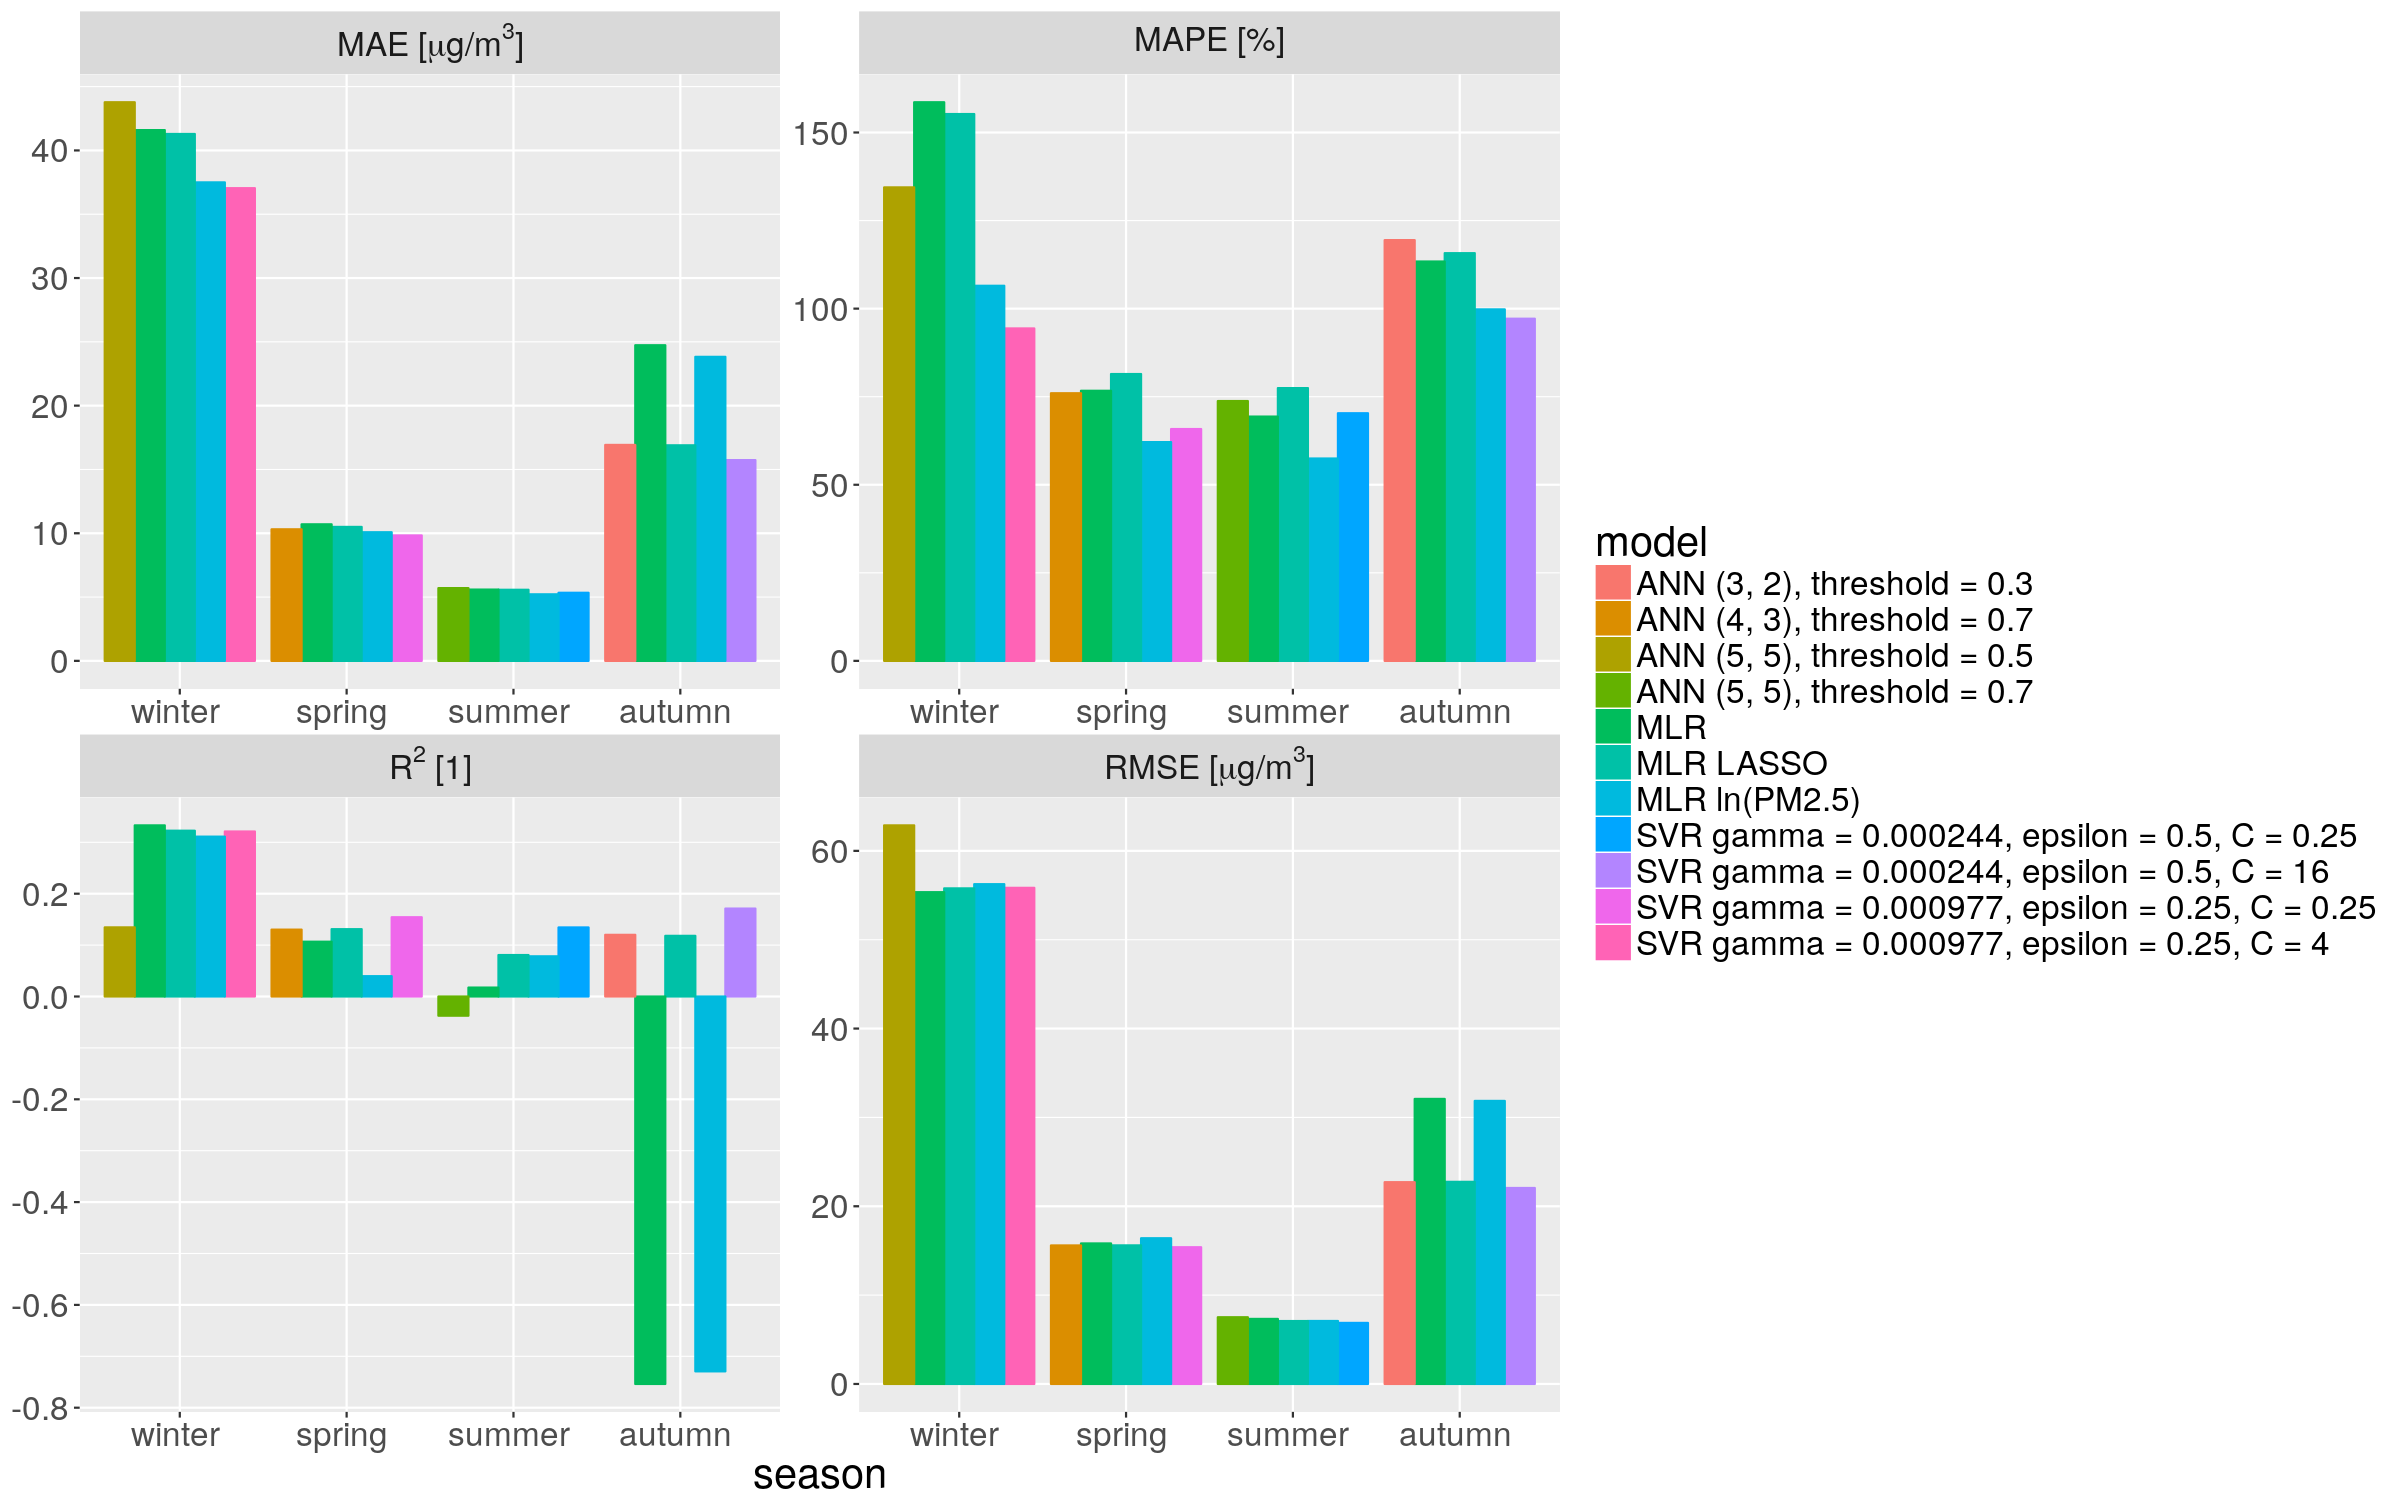
\includegraphics[width=\linewidth]{{figures/results/bujaka_same_season_plot}.png}
\caption{Results of the best models - GIOŚ Bujaka, all data }
\label{fig:results-best-bujaka-all-data}
\end{figure}
\end{landscape}

\begin{landscape}
\begin{figure}[htp]
\centering
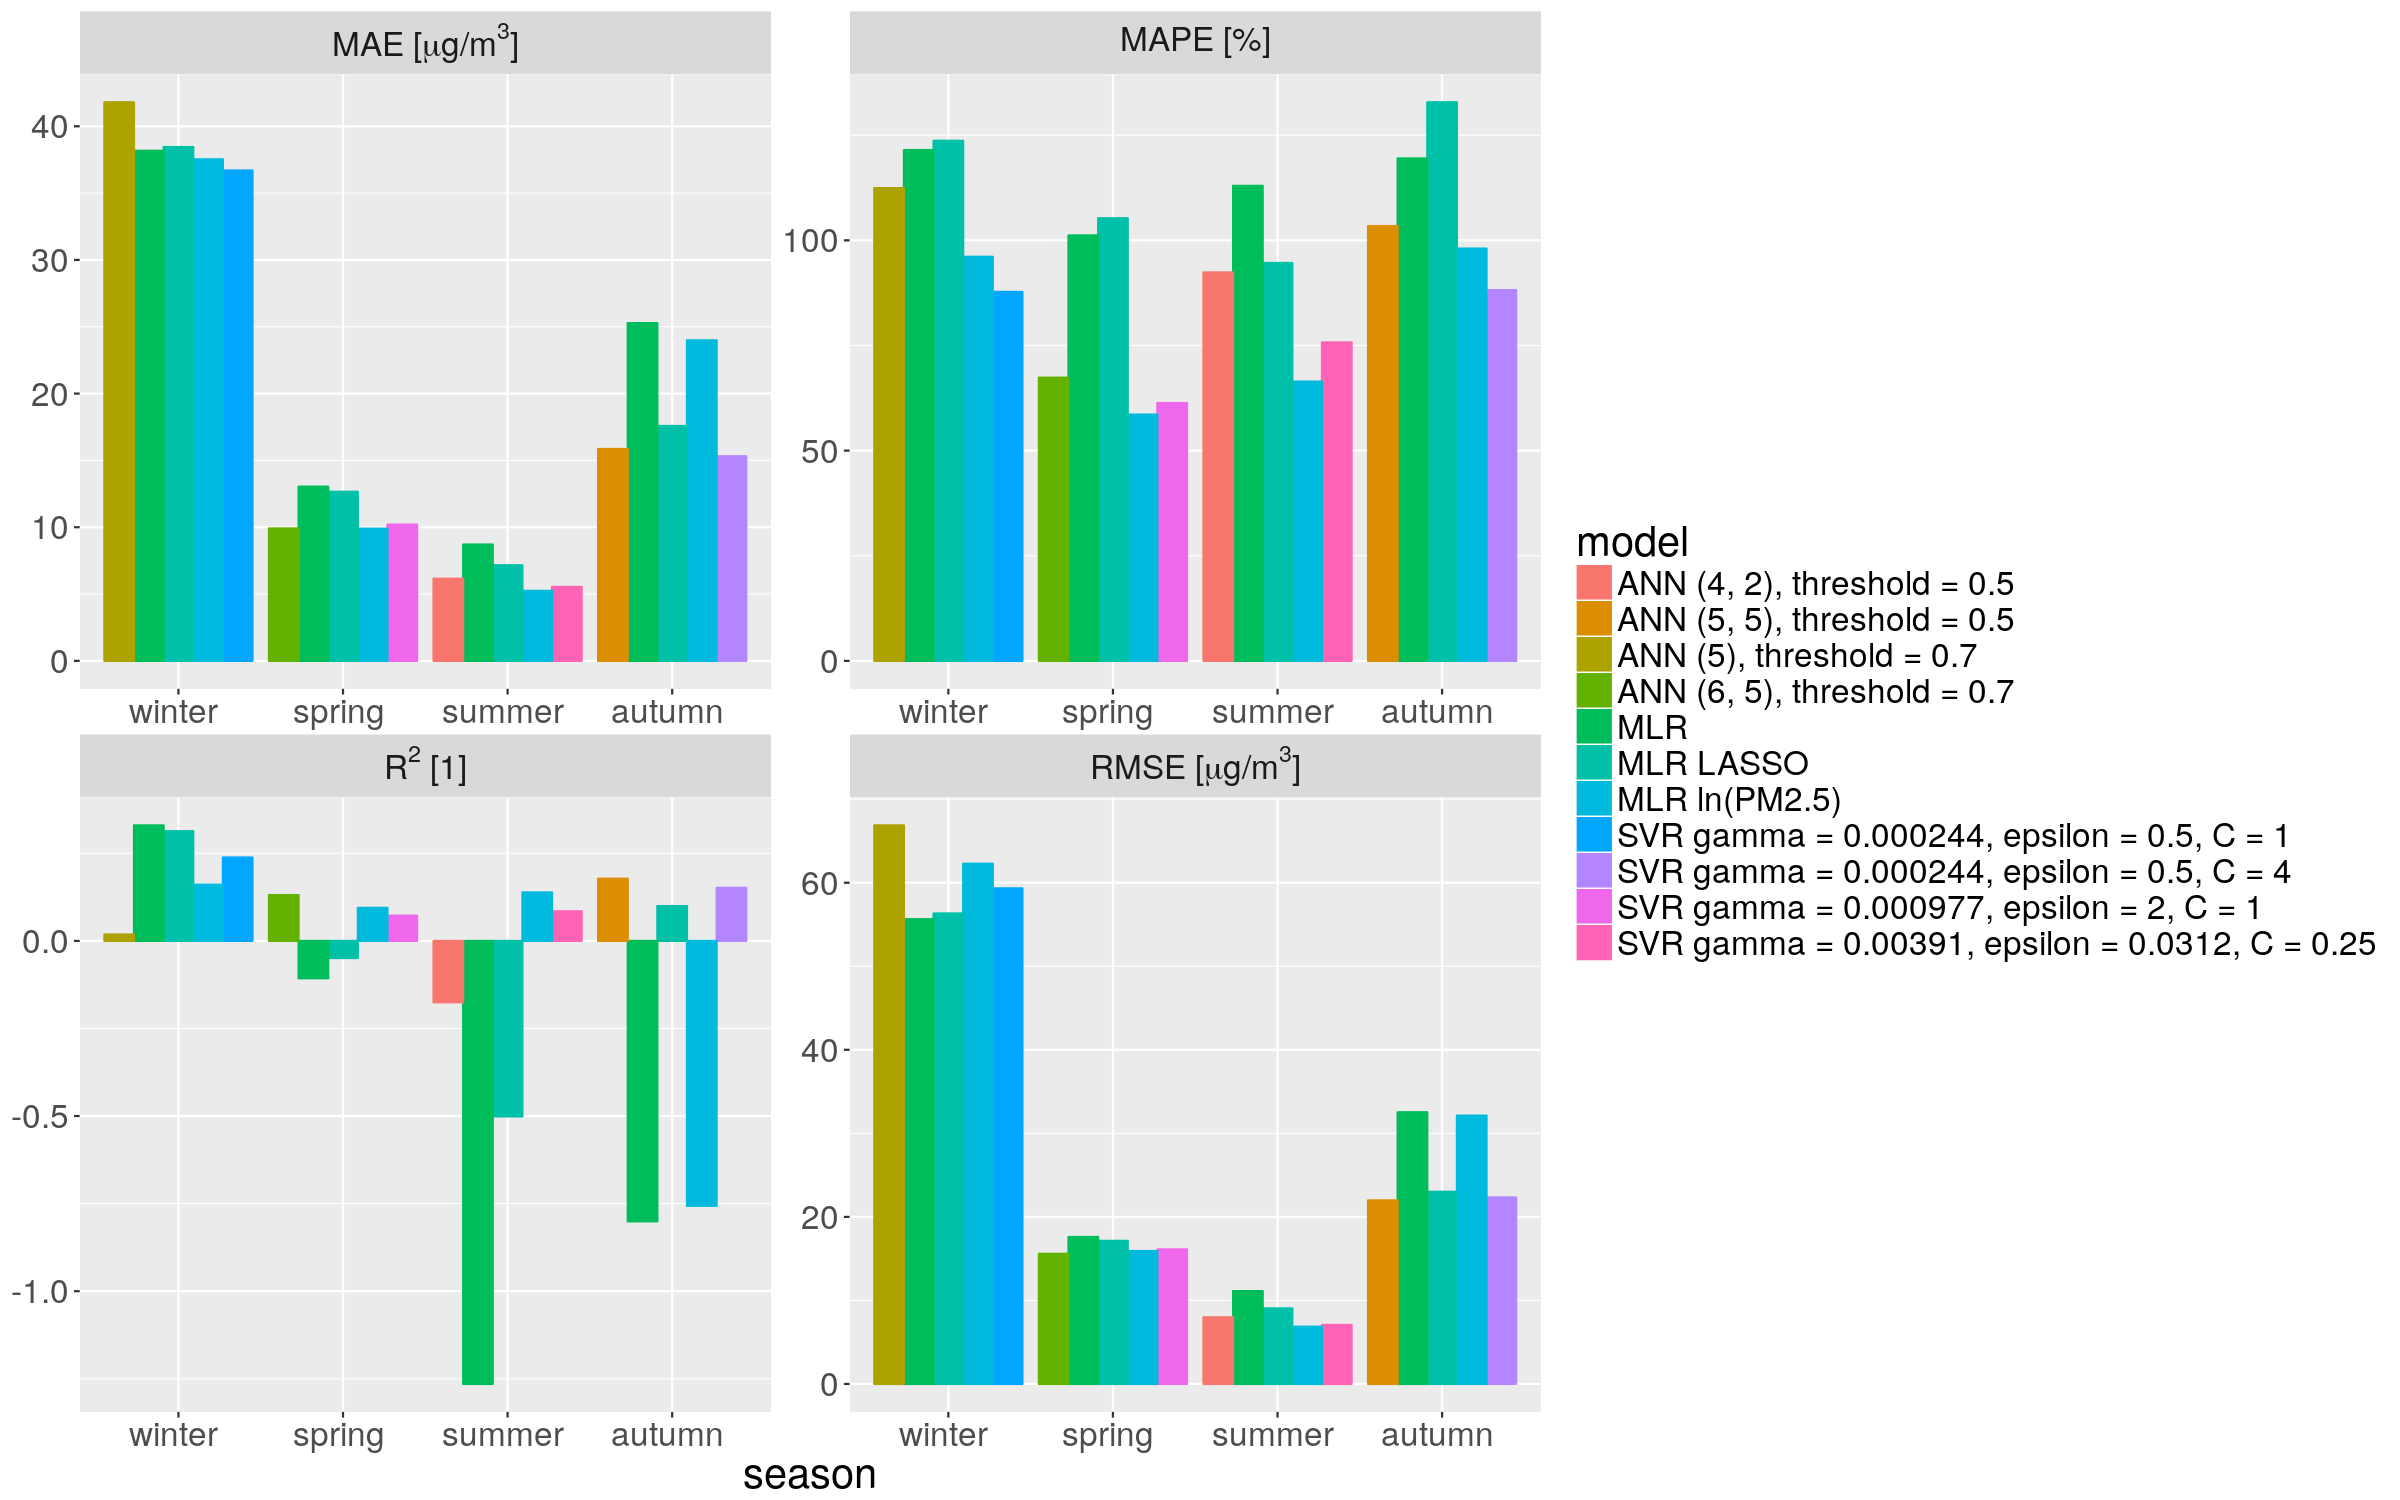
\includegraphics[width=\linewidth]{{figures/results/bujaka_continuous_plot}.png}
\caption{Results of the best models - GIOŚ Bujaka, same season }
\label{fig:results-best-bujaka-same-season}
\end{figure}
\end{landscape}

\begin{landscape}
\begin{figure}[htp]
\centering
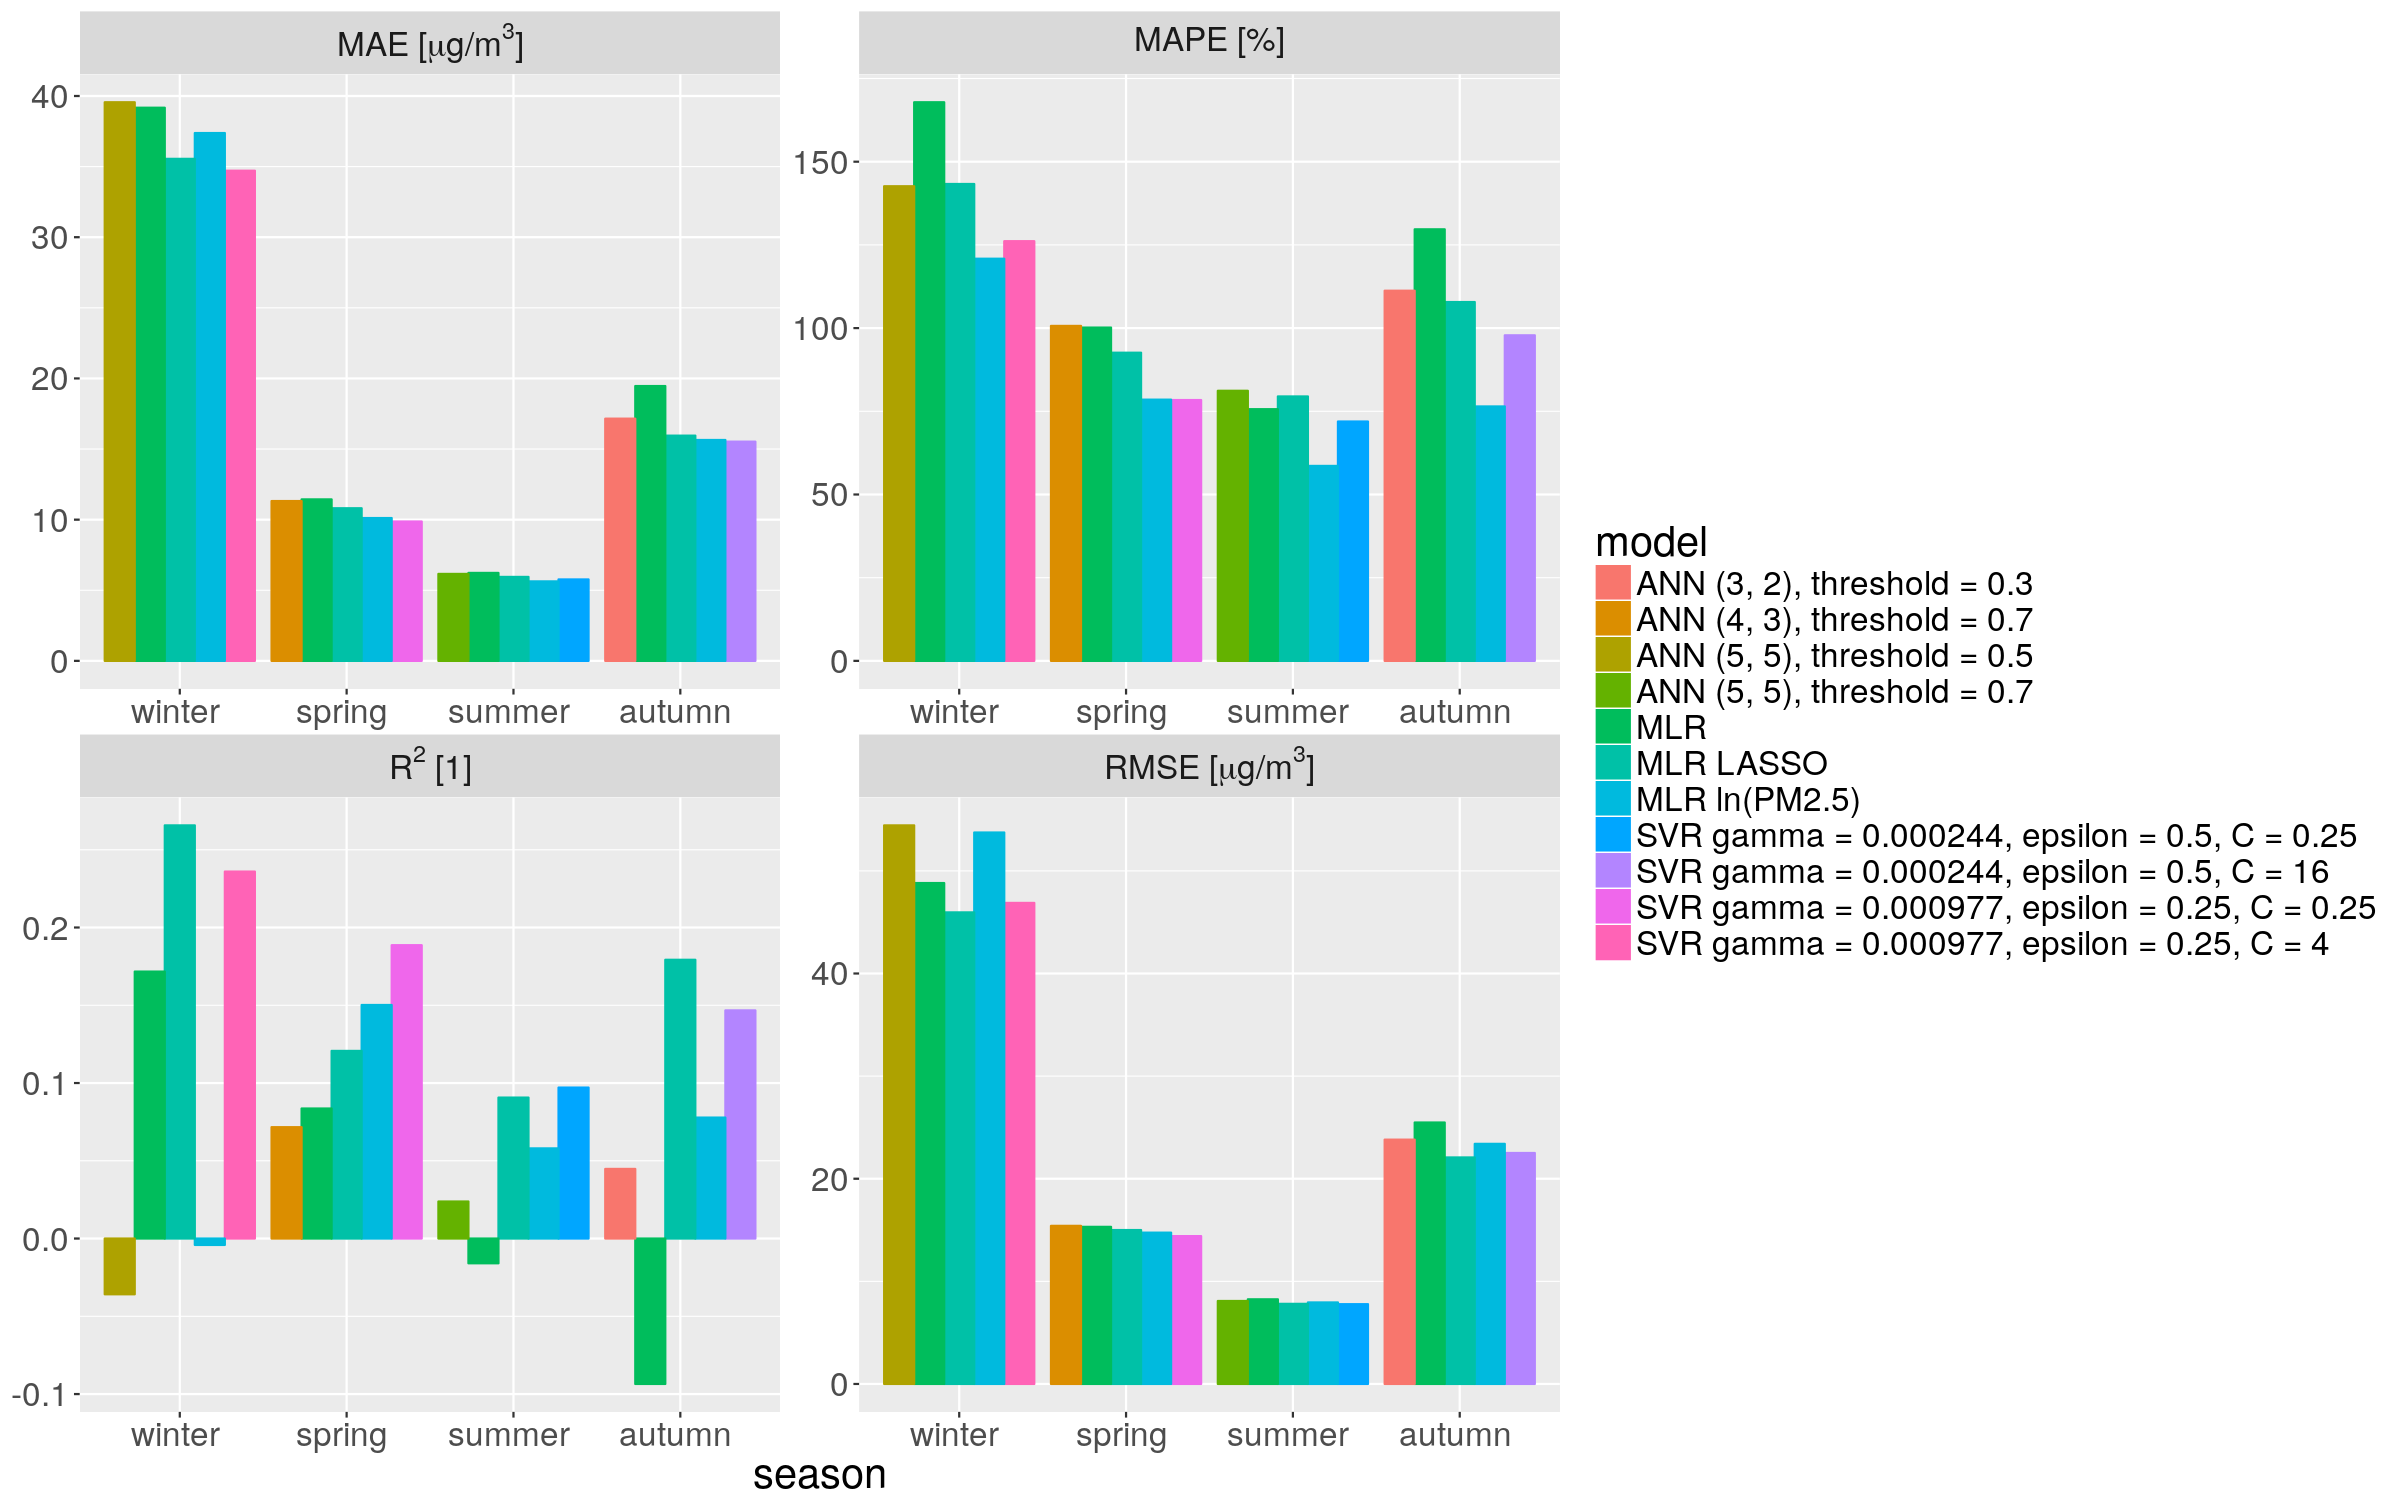
\includegraphics[width=\linewidth]{{figures/results/bulwarowa_same_season_plot}.png}
\caption{Results of the best models - GIOŚ Bulwarowa, all data }
\label{fig:results-best-bulwarowa-all-datat}
\end{figure}
\end{landscape}

\begin{landscape}
\begin{figure}[htp]
\centering
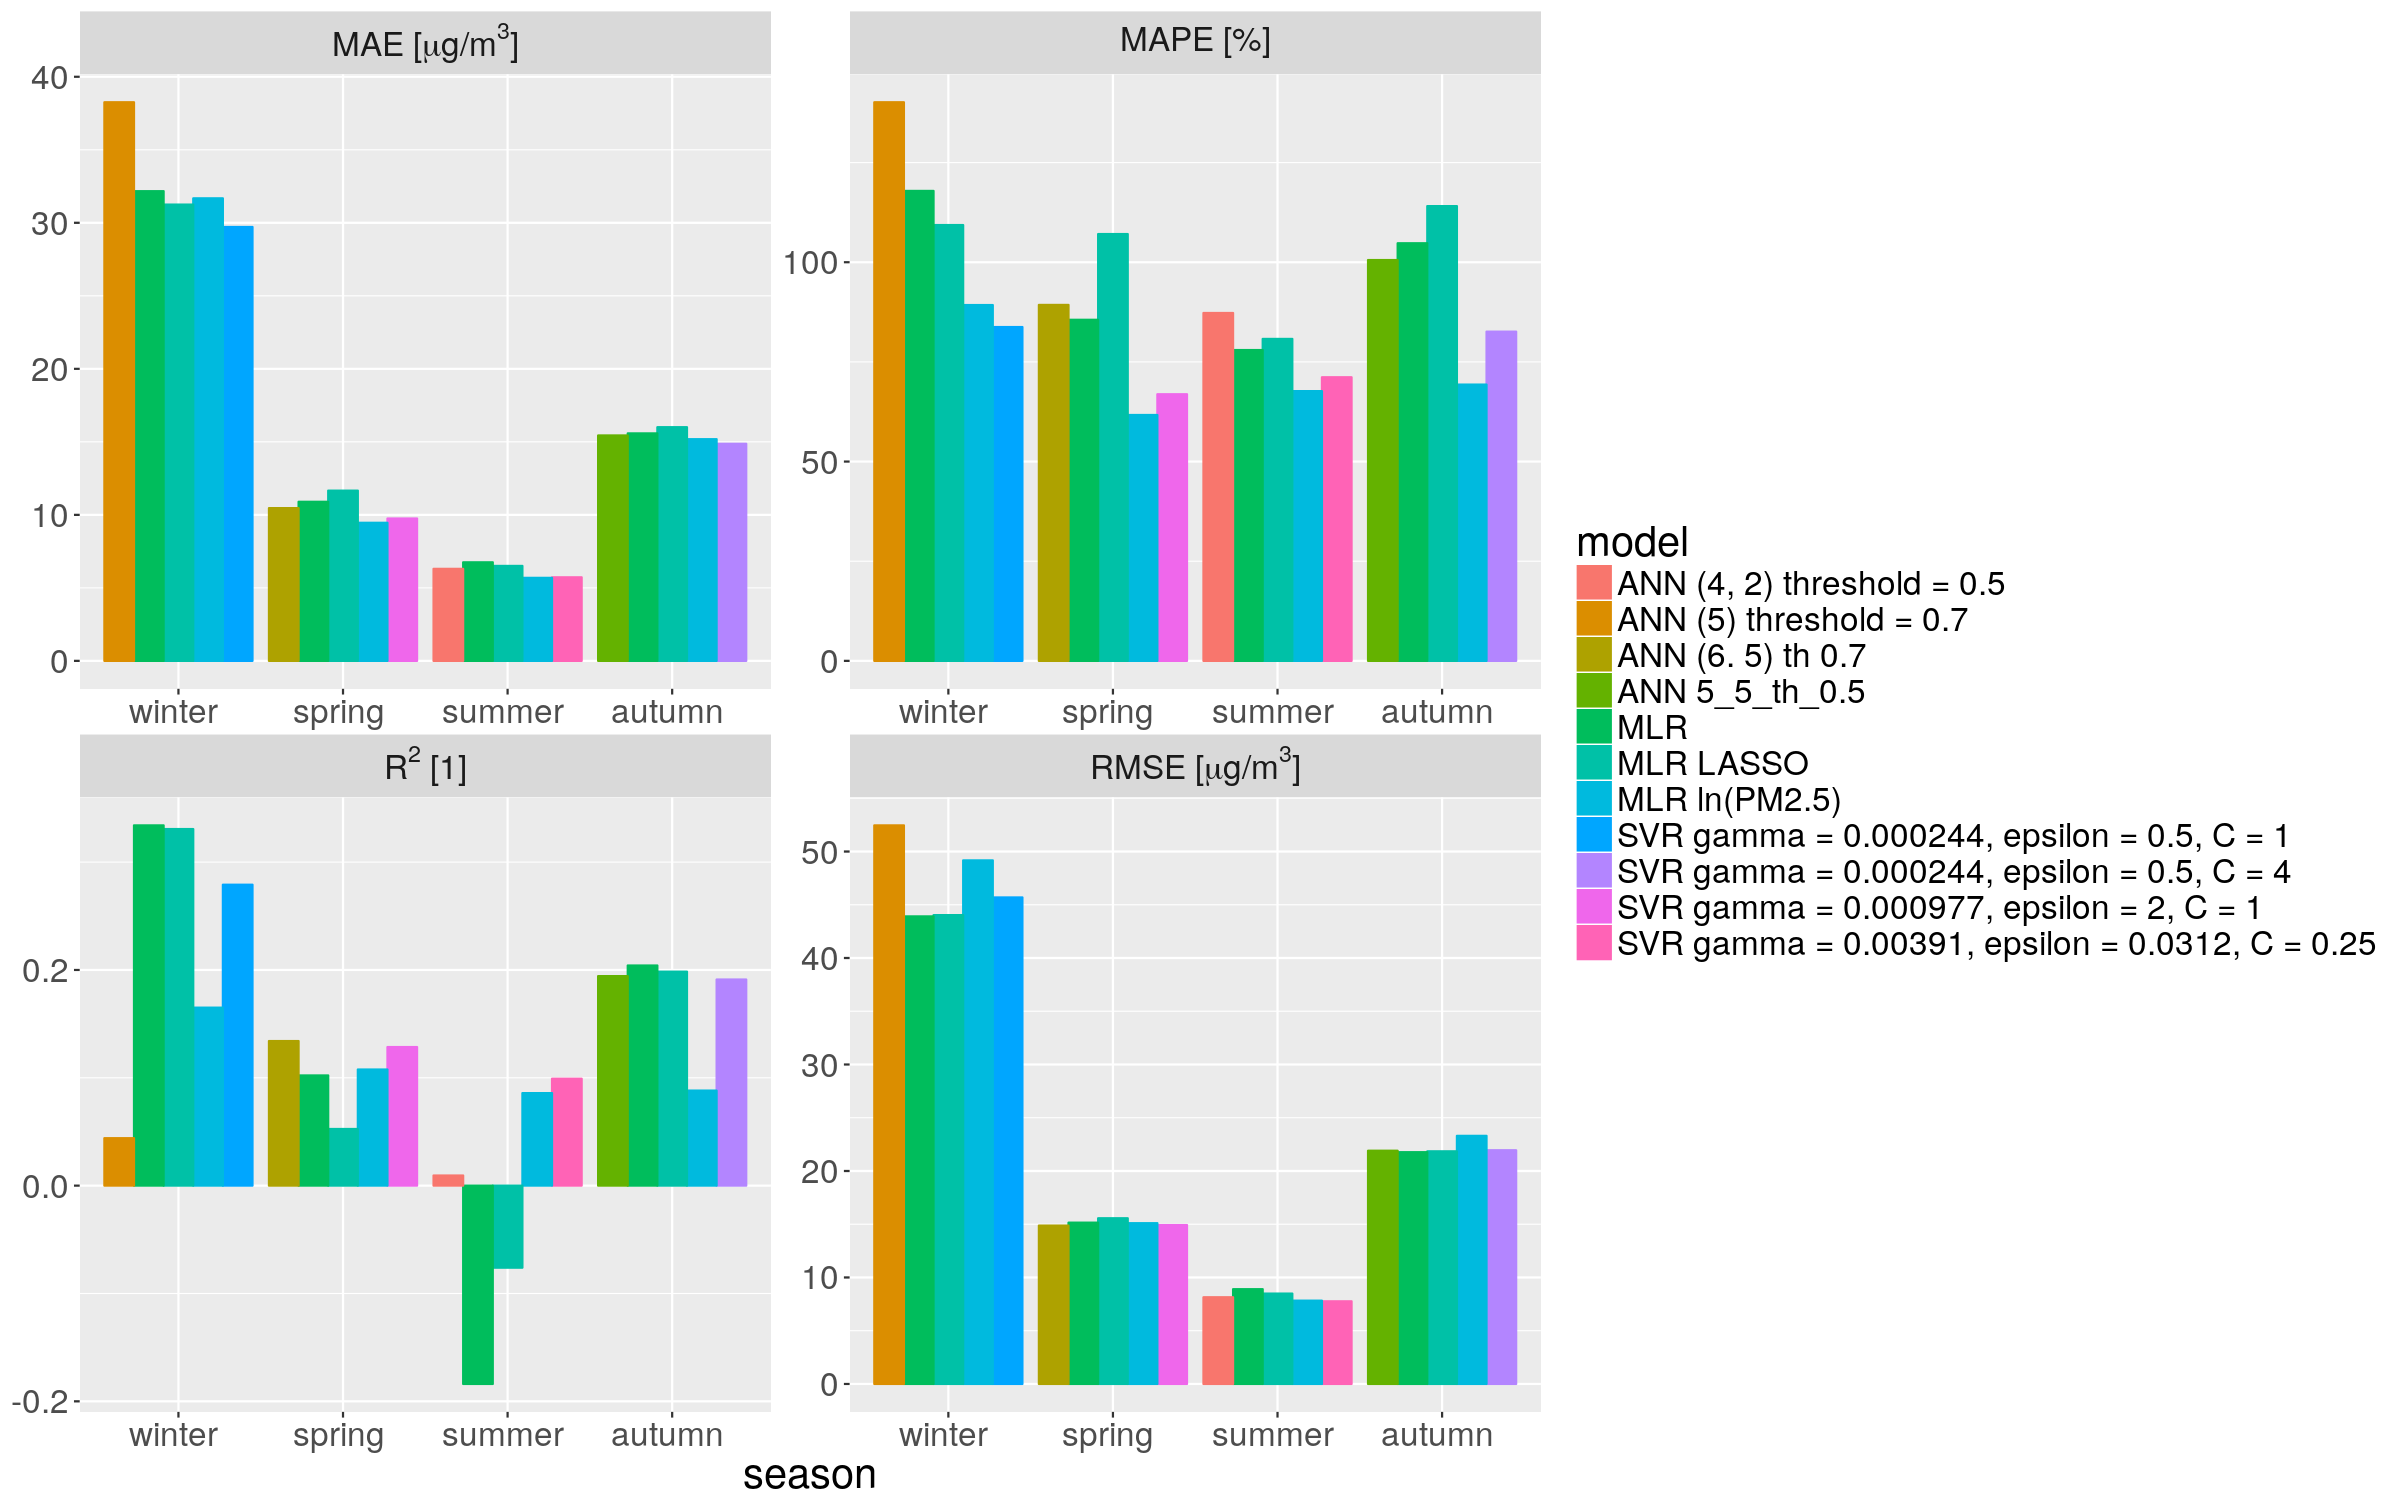
\includegraphics[width=\linewidth]{{figures/results/bulwarowa_continuous_plot}.png}
\caption{Results of the best models - GIOŚ Bulwarowa, same season }
\label{fig:results-best-bulwarowa-same-season}
\end{figure}
\end{landscape}

\begin{landscape}
\begin{figure}[htp]
\centering
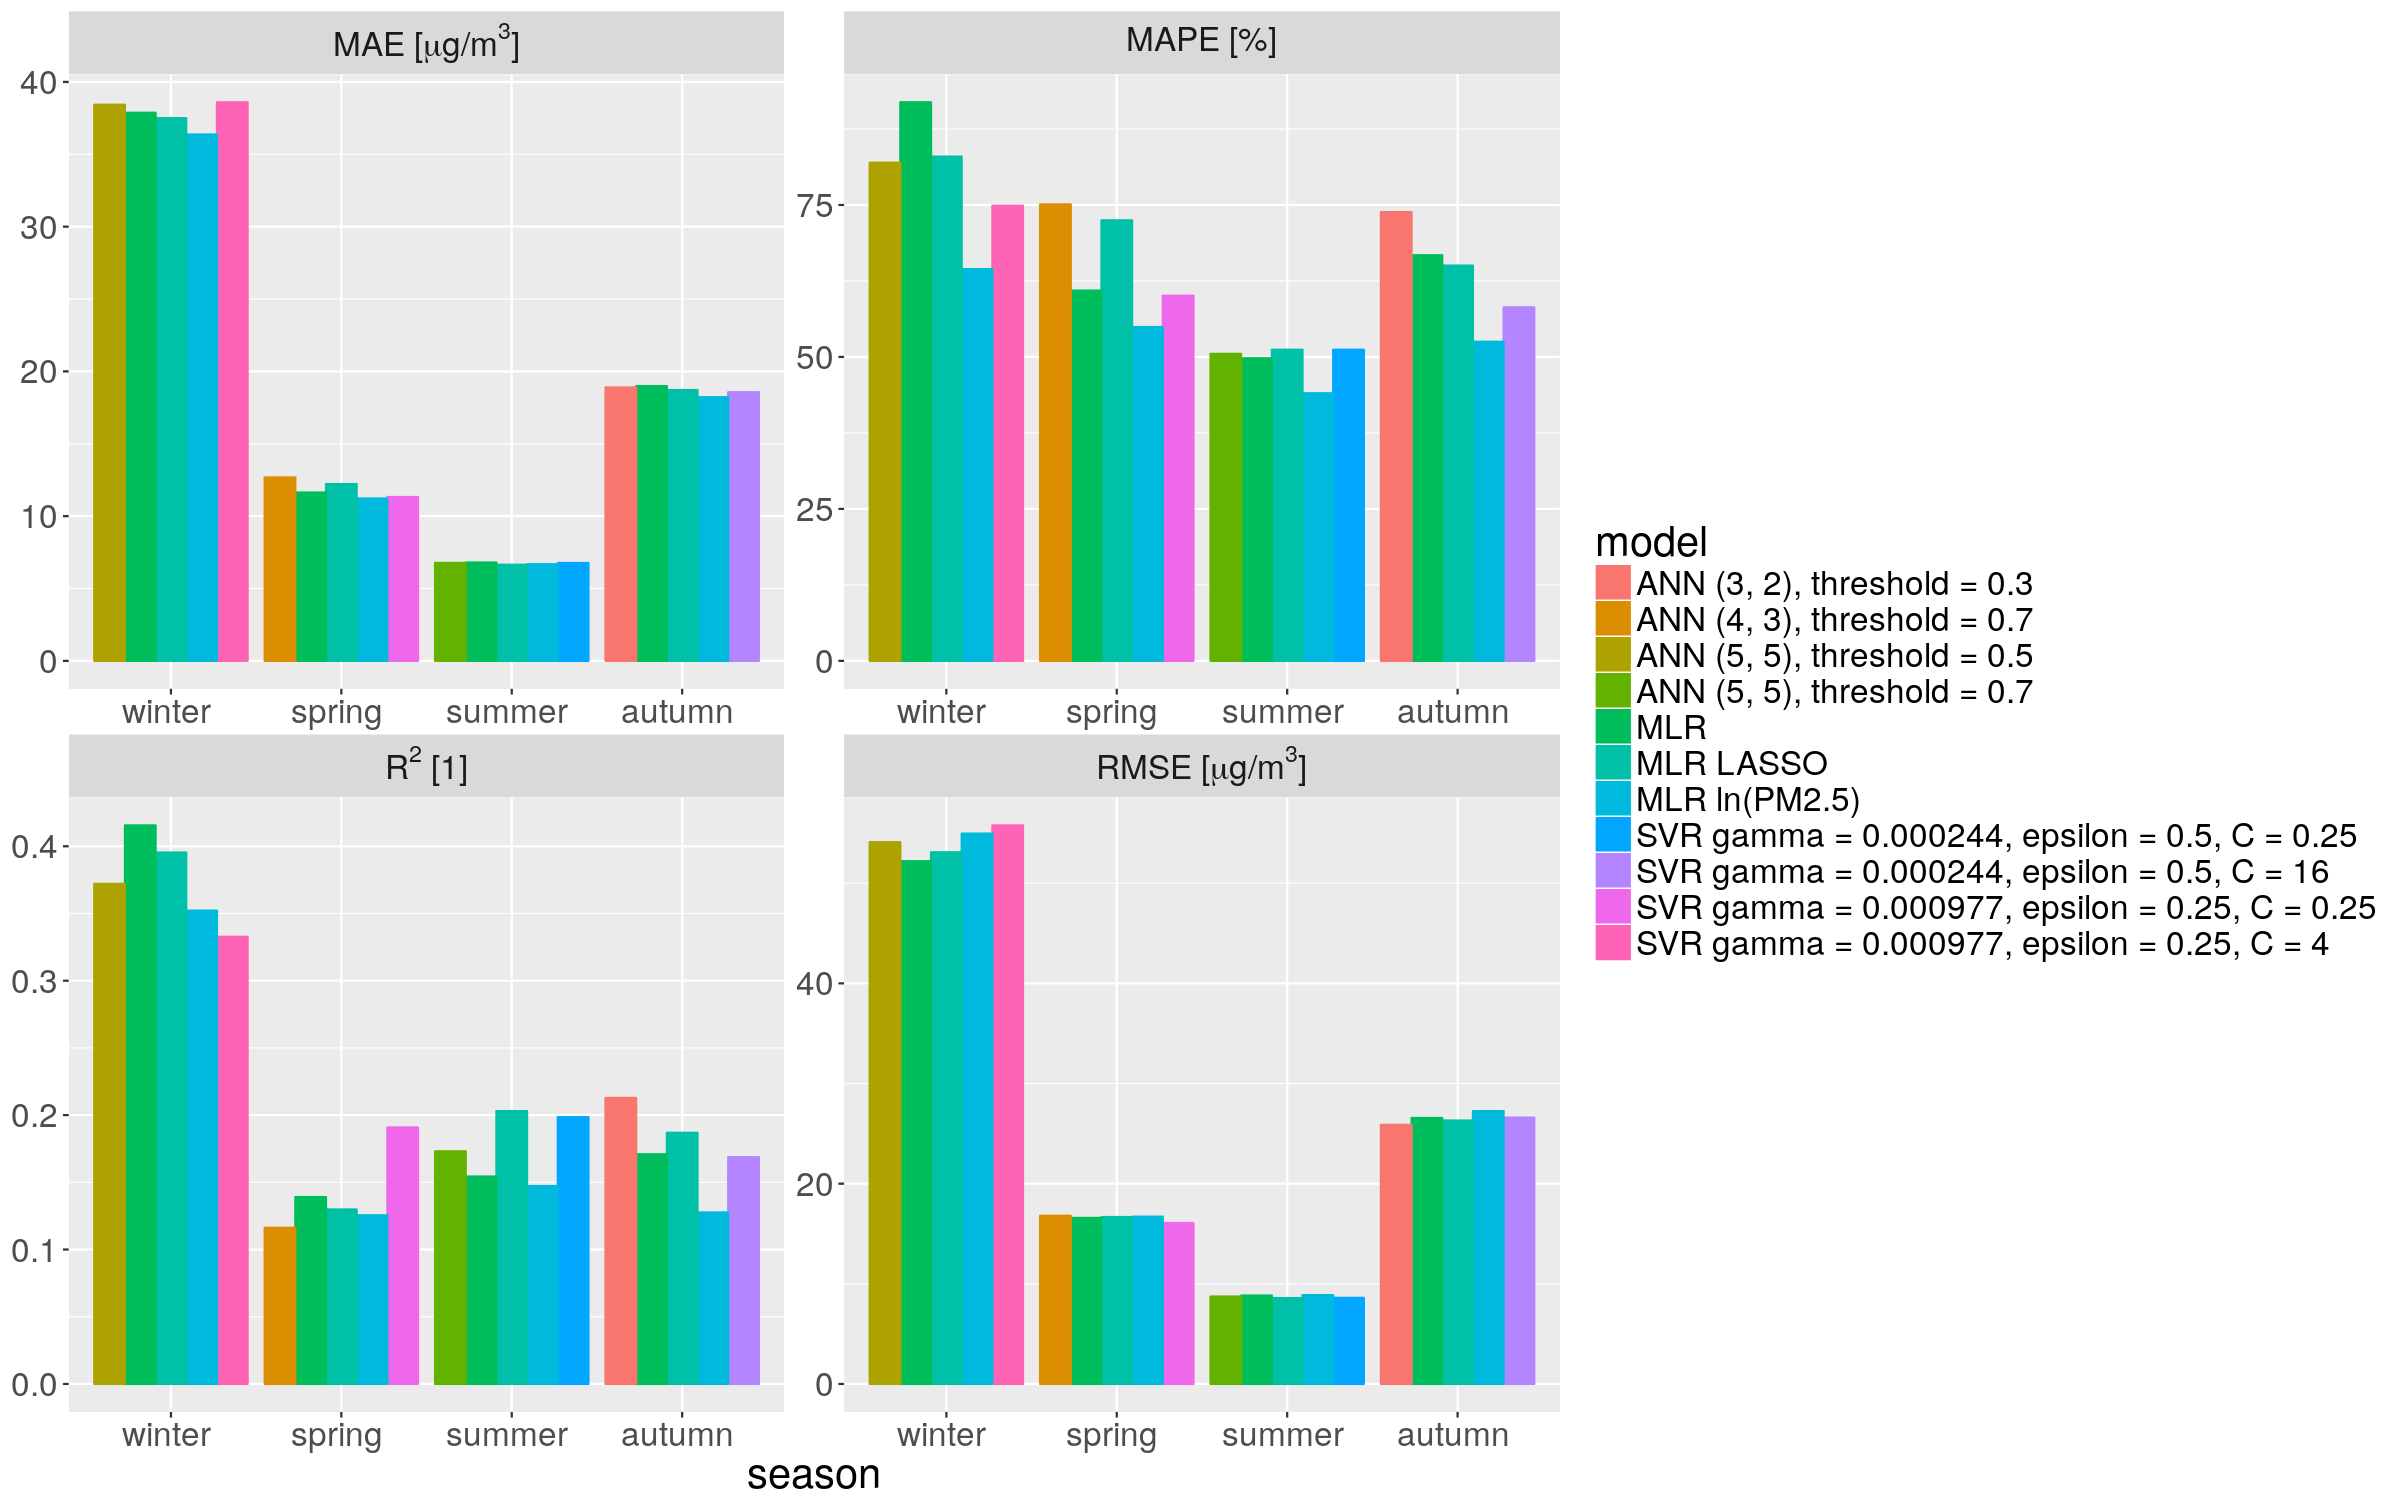
\includegraphics[width=\linewidth]{{figures/results/krasinskiego_same_season_plot}.png}
\caption{Results of the best models - GIOŚ Krasińskiego, all data }
\label{fig:results-best-krasinskiego-all-data}
\end{figure}
\end{landscape}

\begin{landscape}
\begin{figure}[htp]
\centering
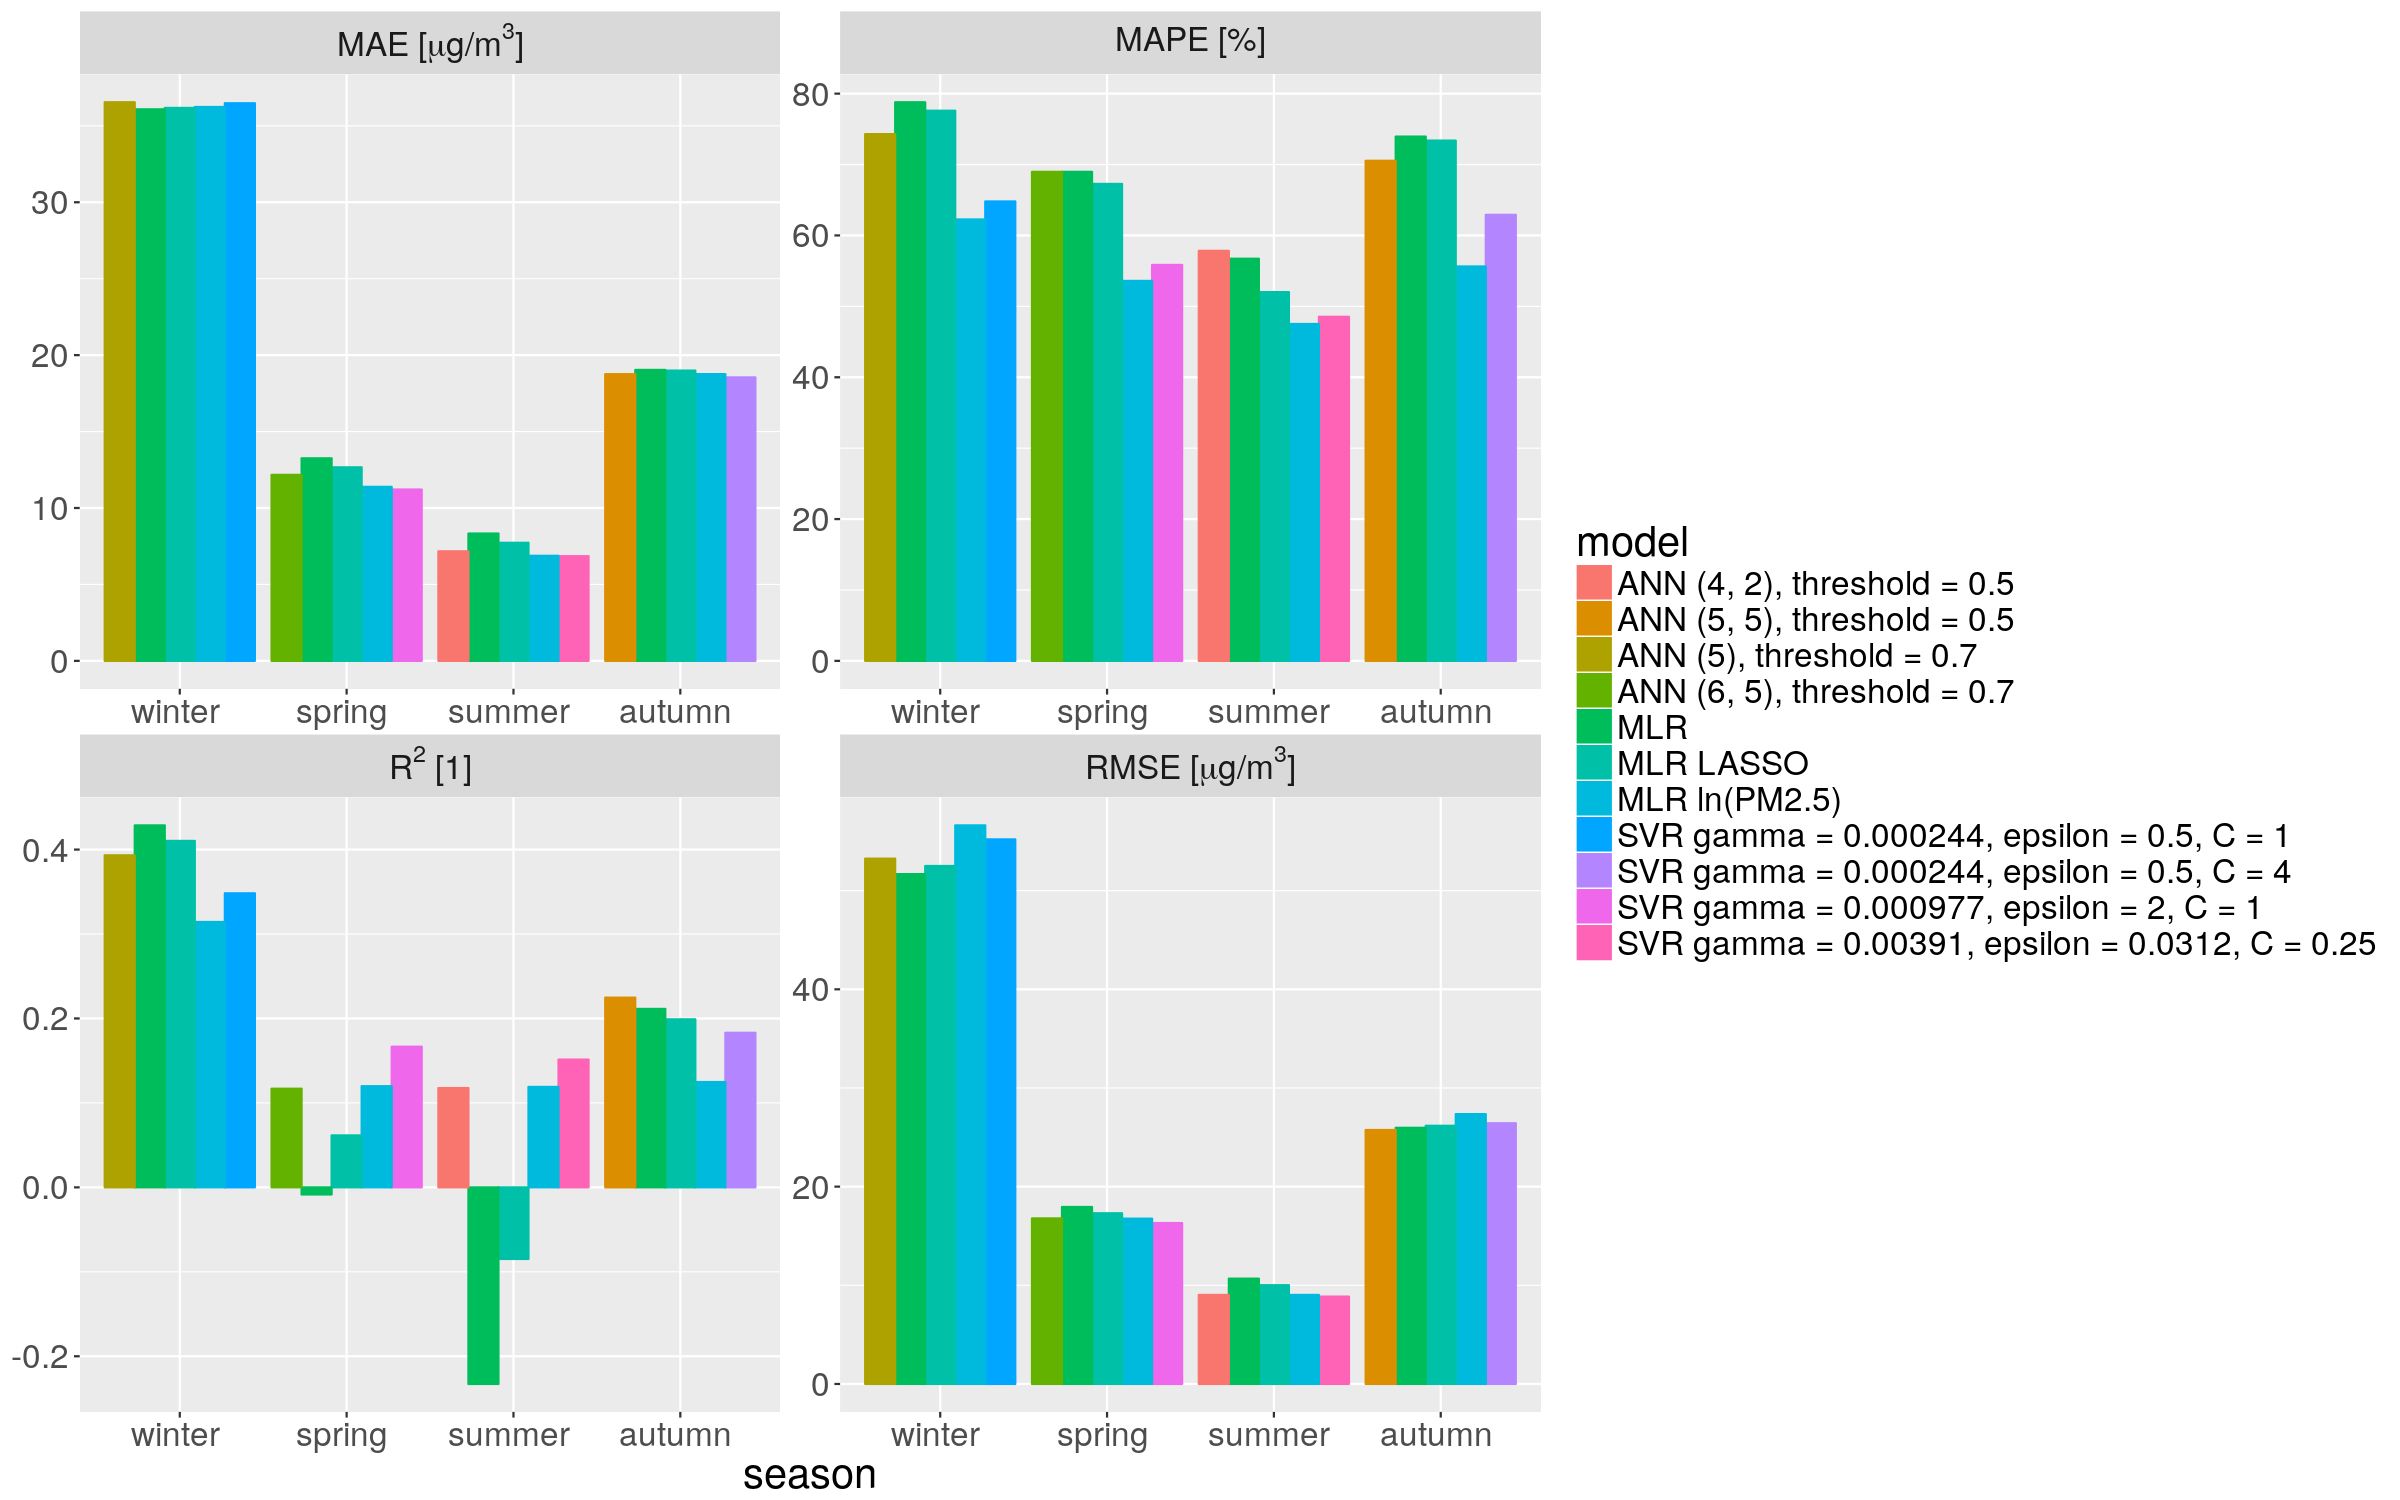
\includegraphics[width=\linewidth]{{figures/results/krasinskiego_continuous_plot}.png}
\caption{Results of the best models - GIOŚ Krasińskiego, same season }
\label{fig:results-best-krasinskiego-same-season}
\end{figure}
\end{landscape}

% comparison of actual and predicted PM2.5 concentrations
% GIOŚ Bujaka

% \begin{landscape}
% \begin{figure}[htp]
% \centering
% \includegraphics[width=\linewidth]{{figures/results/best-models/bujaka/all-data/winter/comparison_plot_mlr_lag_24}.png}
% \caption{Comparison of actual and predicted PM2.5 concentrations - GIOŚ Bujaka, winter, all data }
% \label{fig:results-comparison-bujaka-winter-all-data}
% \end{figure}
% \end{landscape}

% \begin{landscape}
% \begin{figure}[htp]
% \centering
% 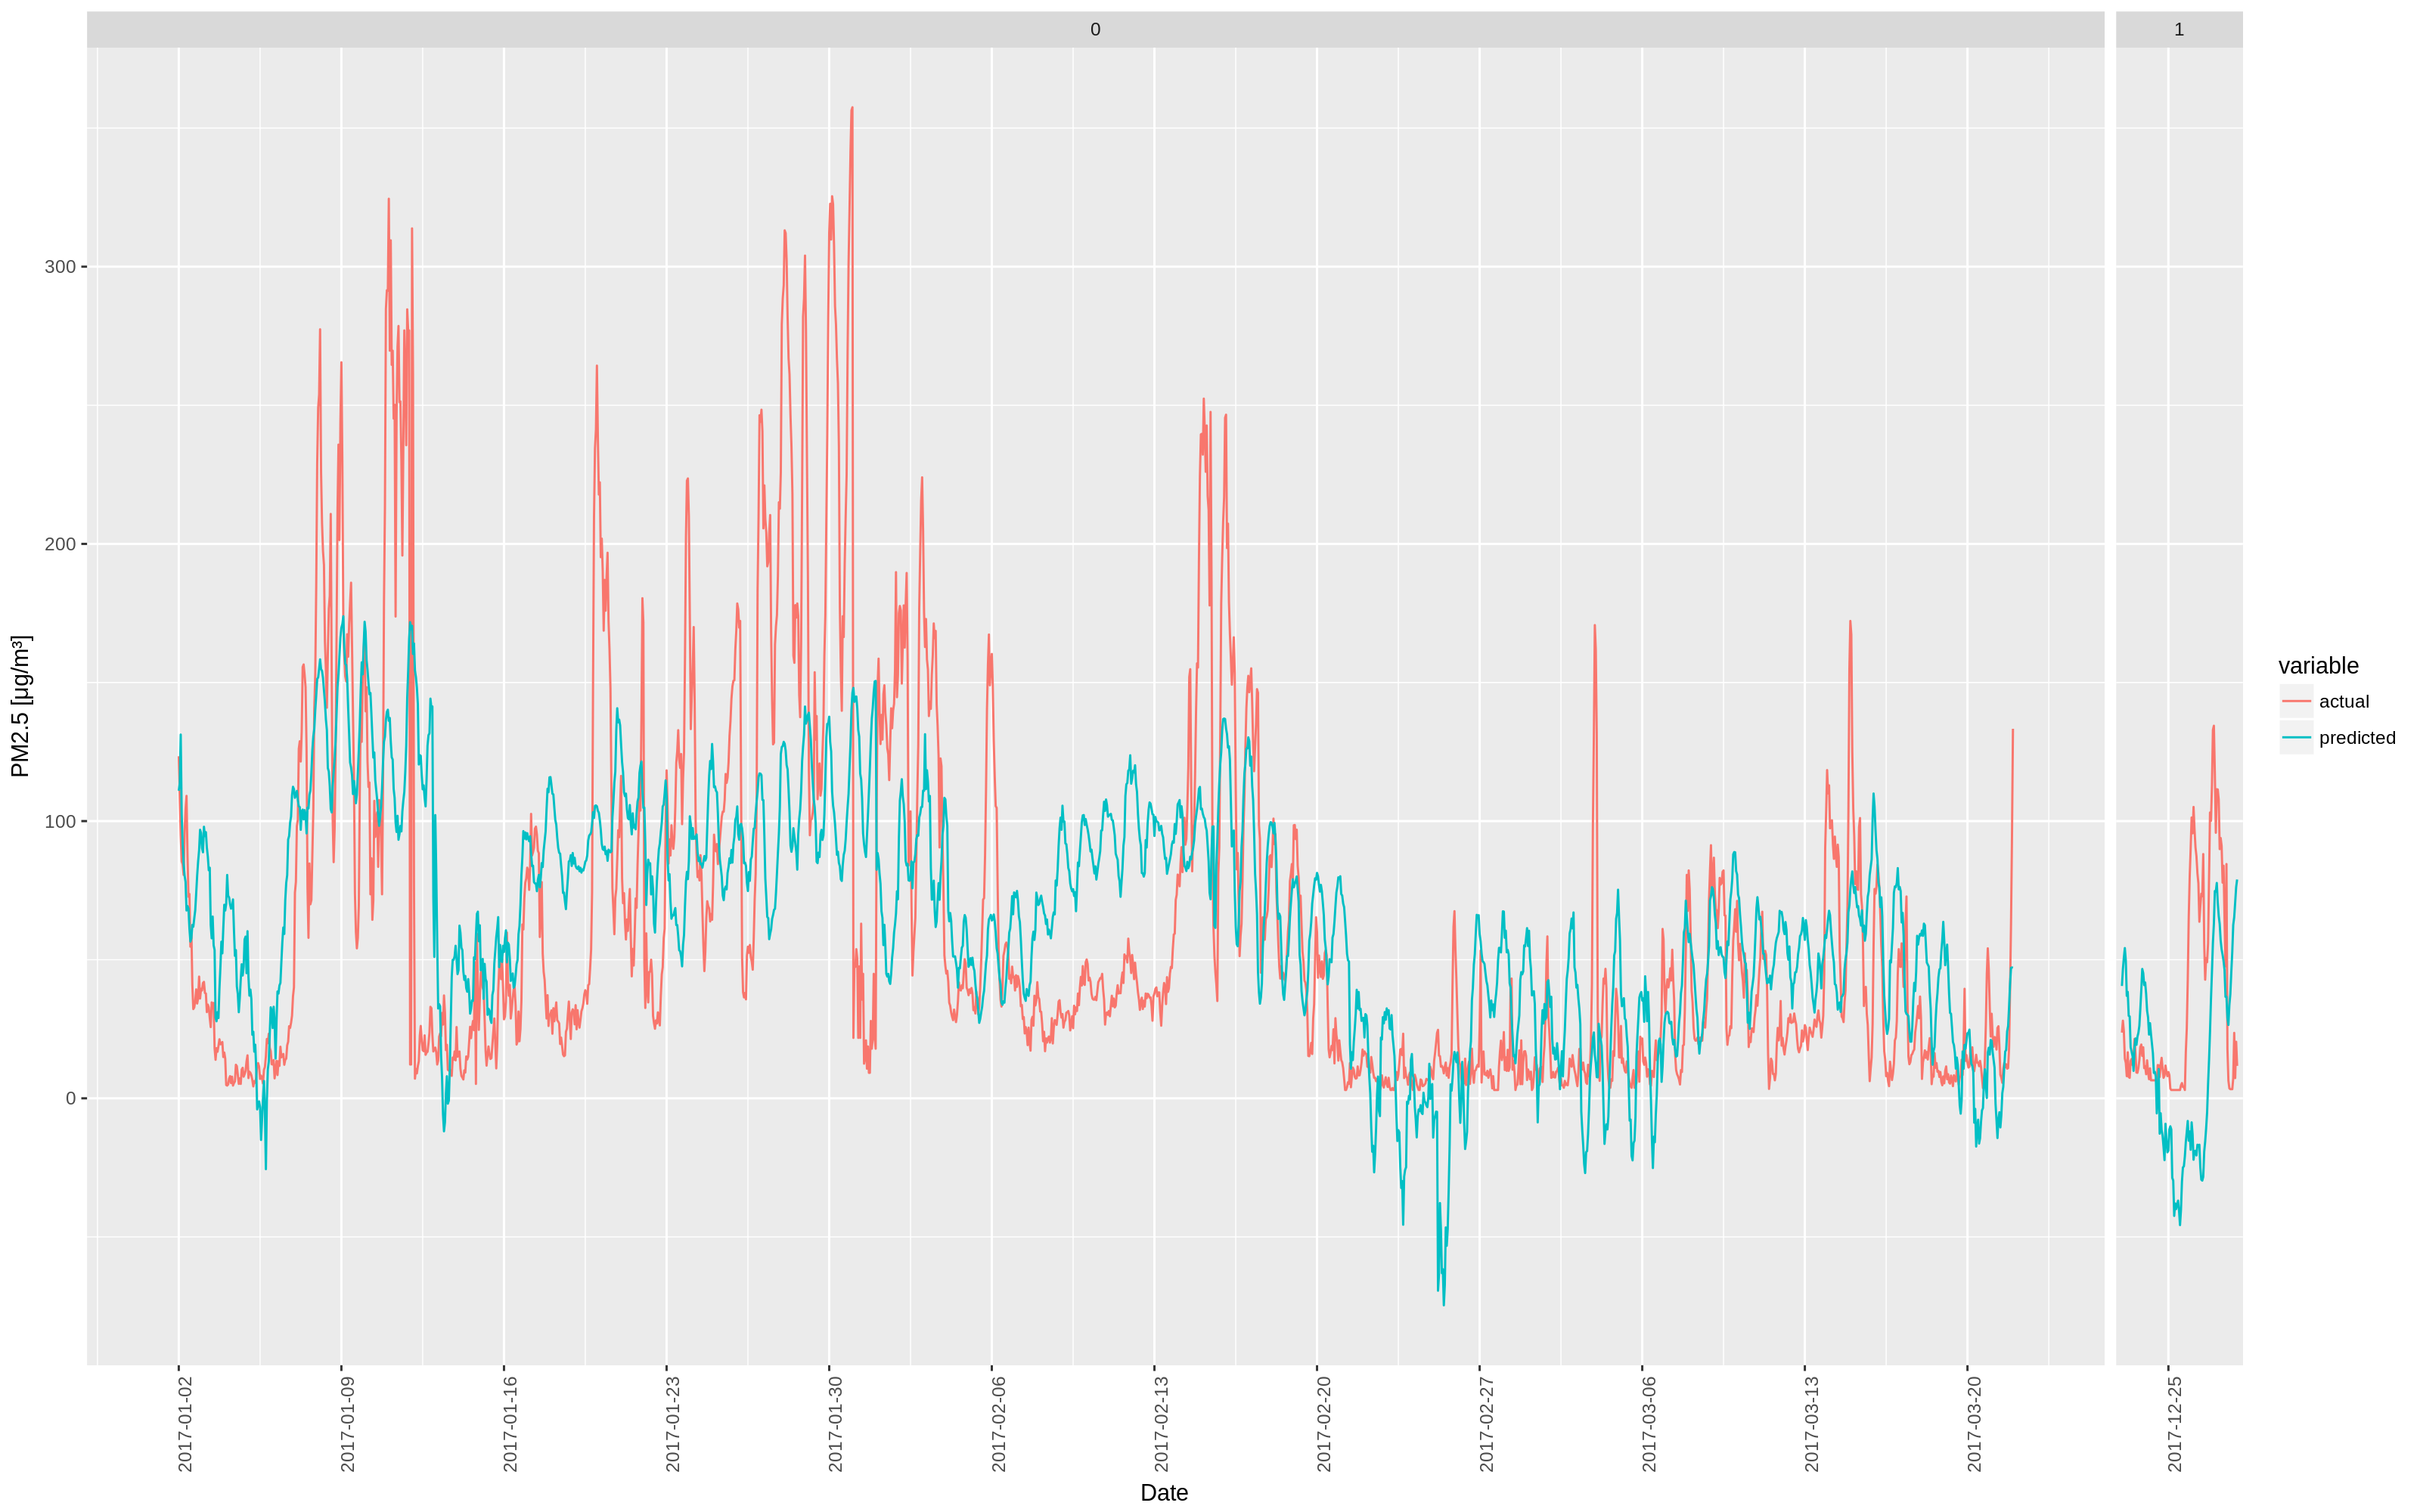
\includegraphics[width=\linewidth]{{figures/results/best-models/bujaka/same-season/winter/all_comparison_plot_mlr_lag_24}.png}
% \caption{Comparison of actual and predicted PM2.5 concentrations - GIOŚ Bujaka, winter, same season }
% \label{fig:results-comparison-bujaka-winter-same-season}
% \end{figure}
% \end{landscape}

% \begin{landscape}
% \begin{figure}[htp]
% \centering
% 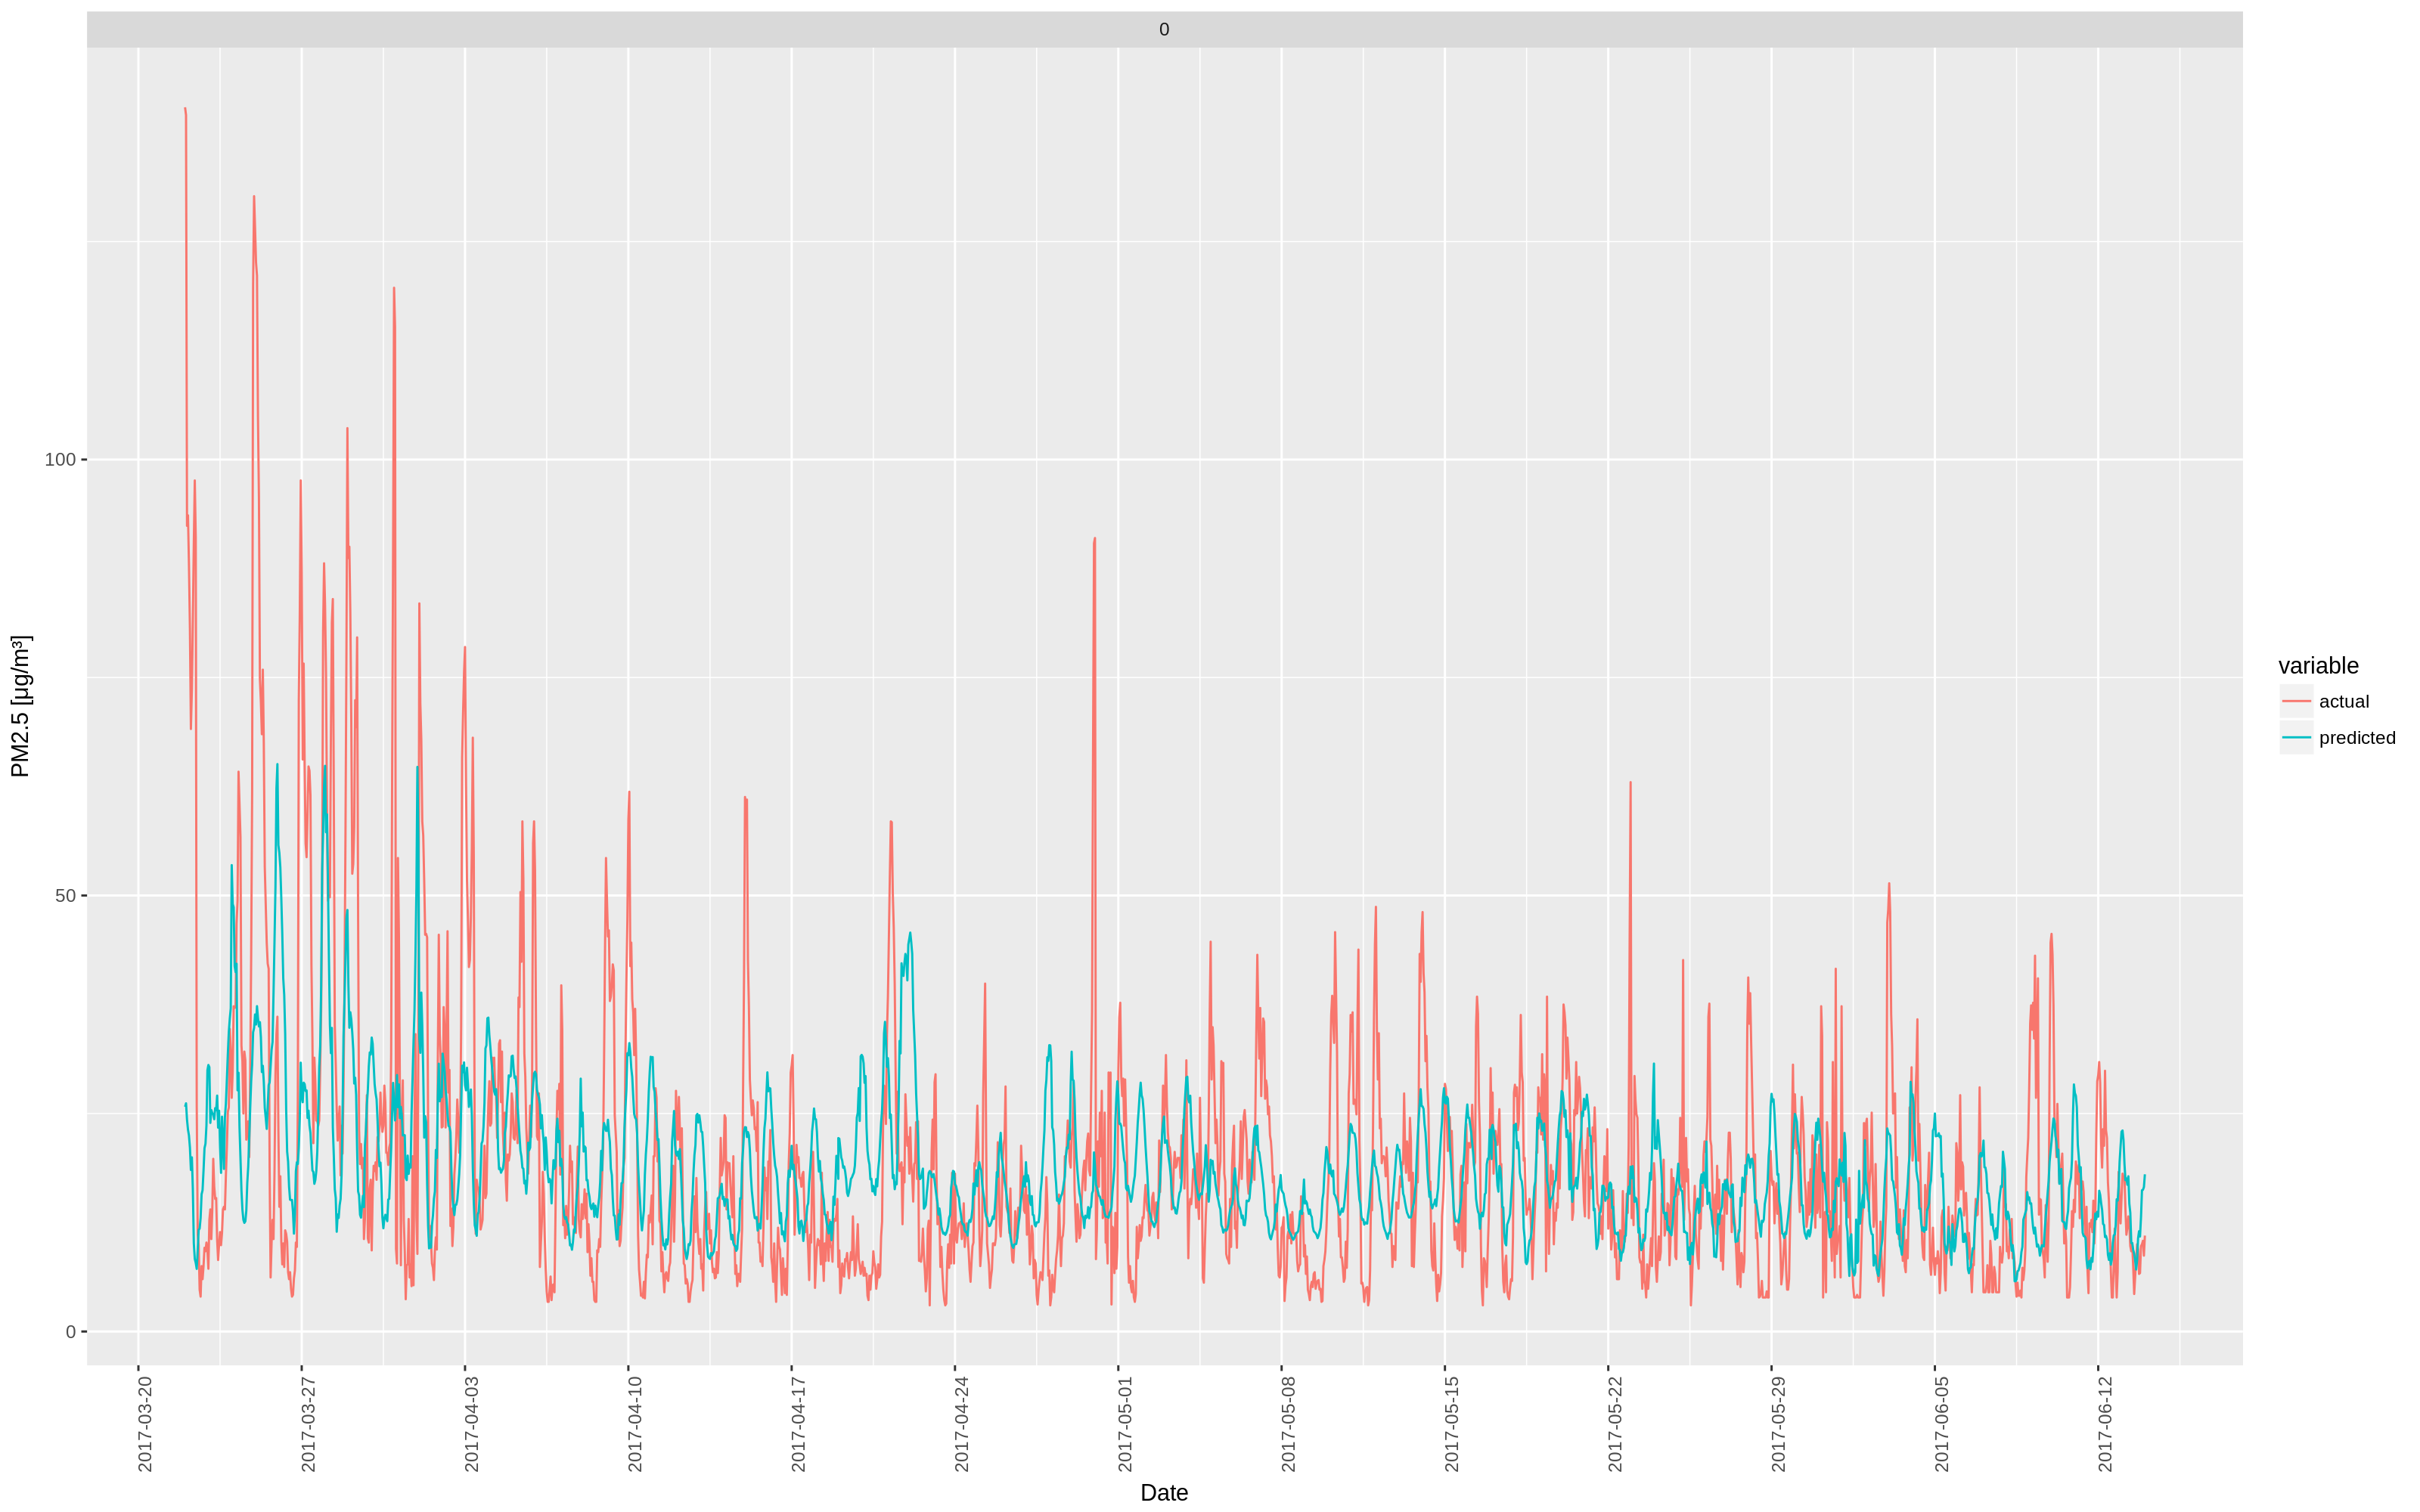
\includegraphics[width=\linewidth]{{figures/results/best-models/bujaka/all-data/spring/comparison_plot_mlp1_6_5_th_9.7_lag_24}.png}
% \caption{Comparison of actual and predicted PM2.5 concentrations - GIOŚ Bujaka, spring, all data }
% \label{fig:results-comparison-bujaka-spring-all-data}
% \end{figure}
% \end{landscape}

% \begin{landscape}
% \begin{figure}[htp]
% \centering
% \includegraphics[width=\linewidth]{{figures/results/best-models/bujaka/same-season/spring/all_comparison_plot_svr_gam0.000977_eps0.25_c0.25_lag_24}.png}
% \caption{Comparison of actual and predicted PM2.5 concentrations - GIOŚ Bujaka, spring, same season }
% \label{fig:results-comparison-bujaka-spring-same-season}
% \end{figure}
% \end{landscape}

% \begin{landscape}
% \begin{figure}[htp]
% \centering
% 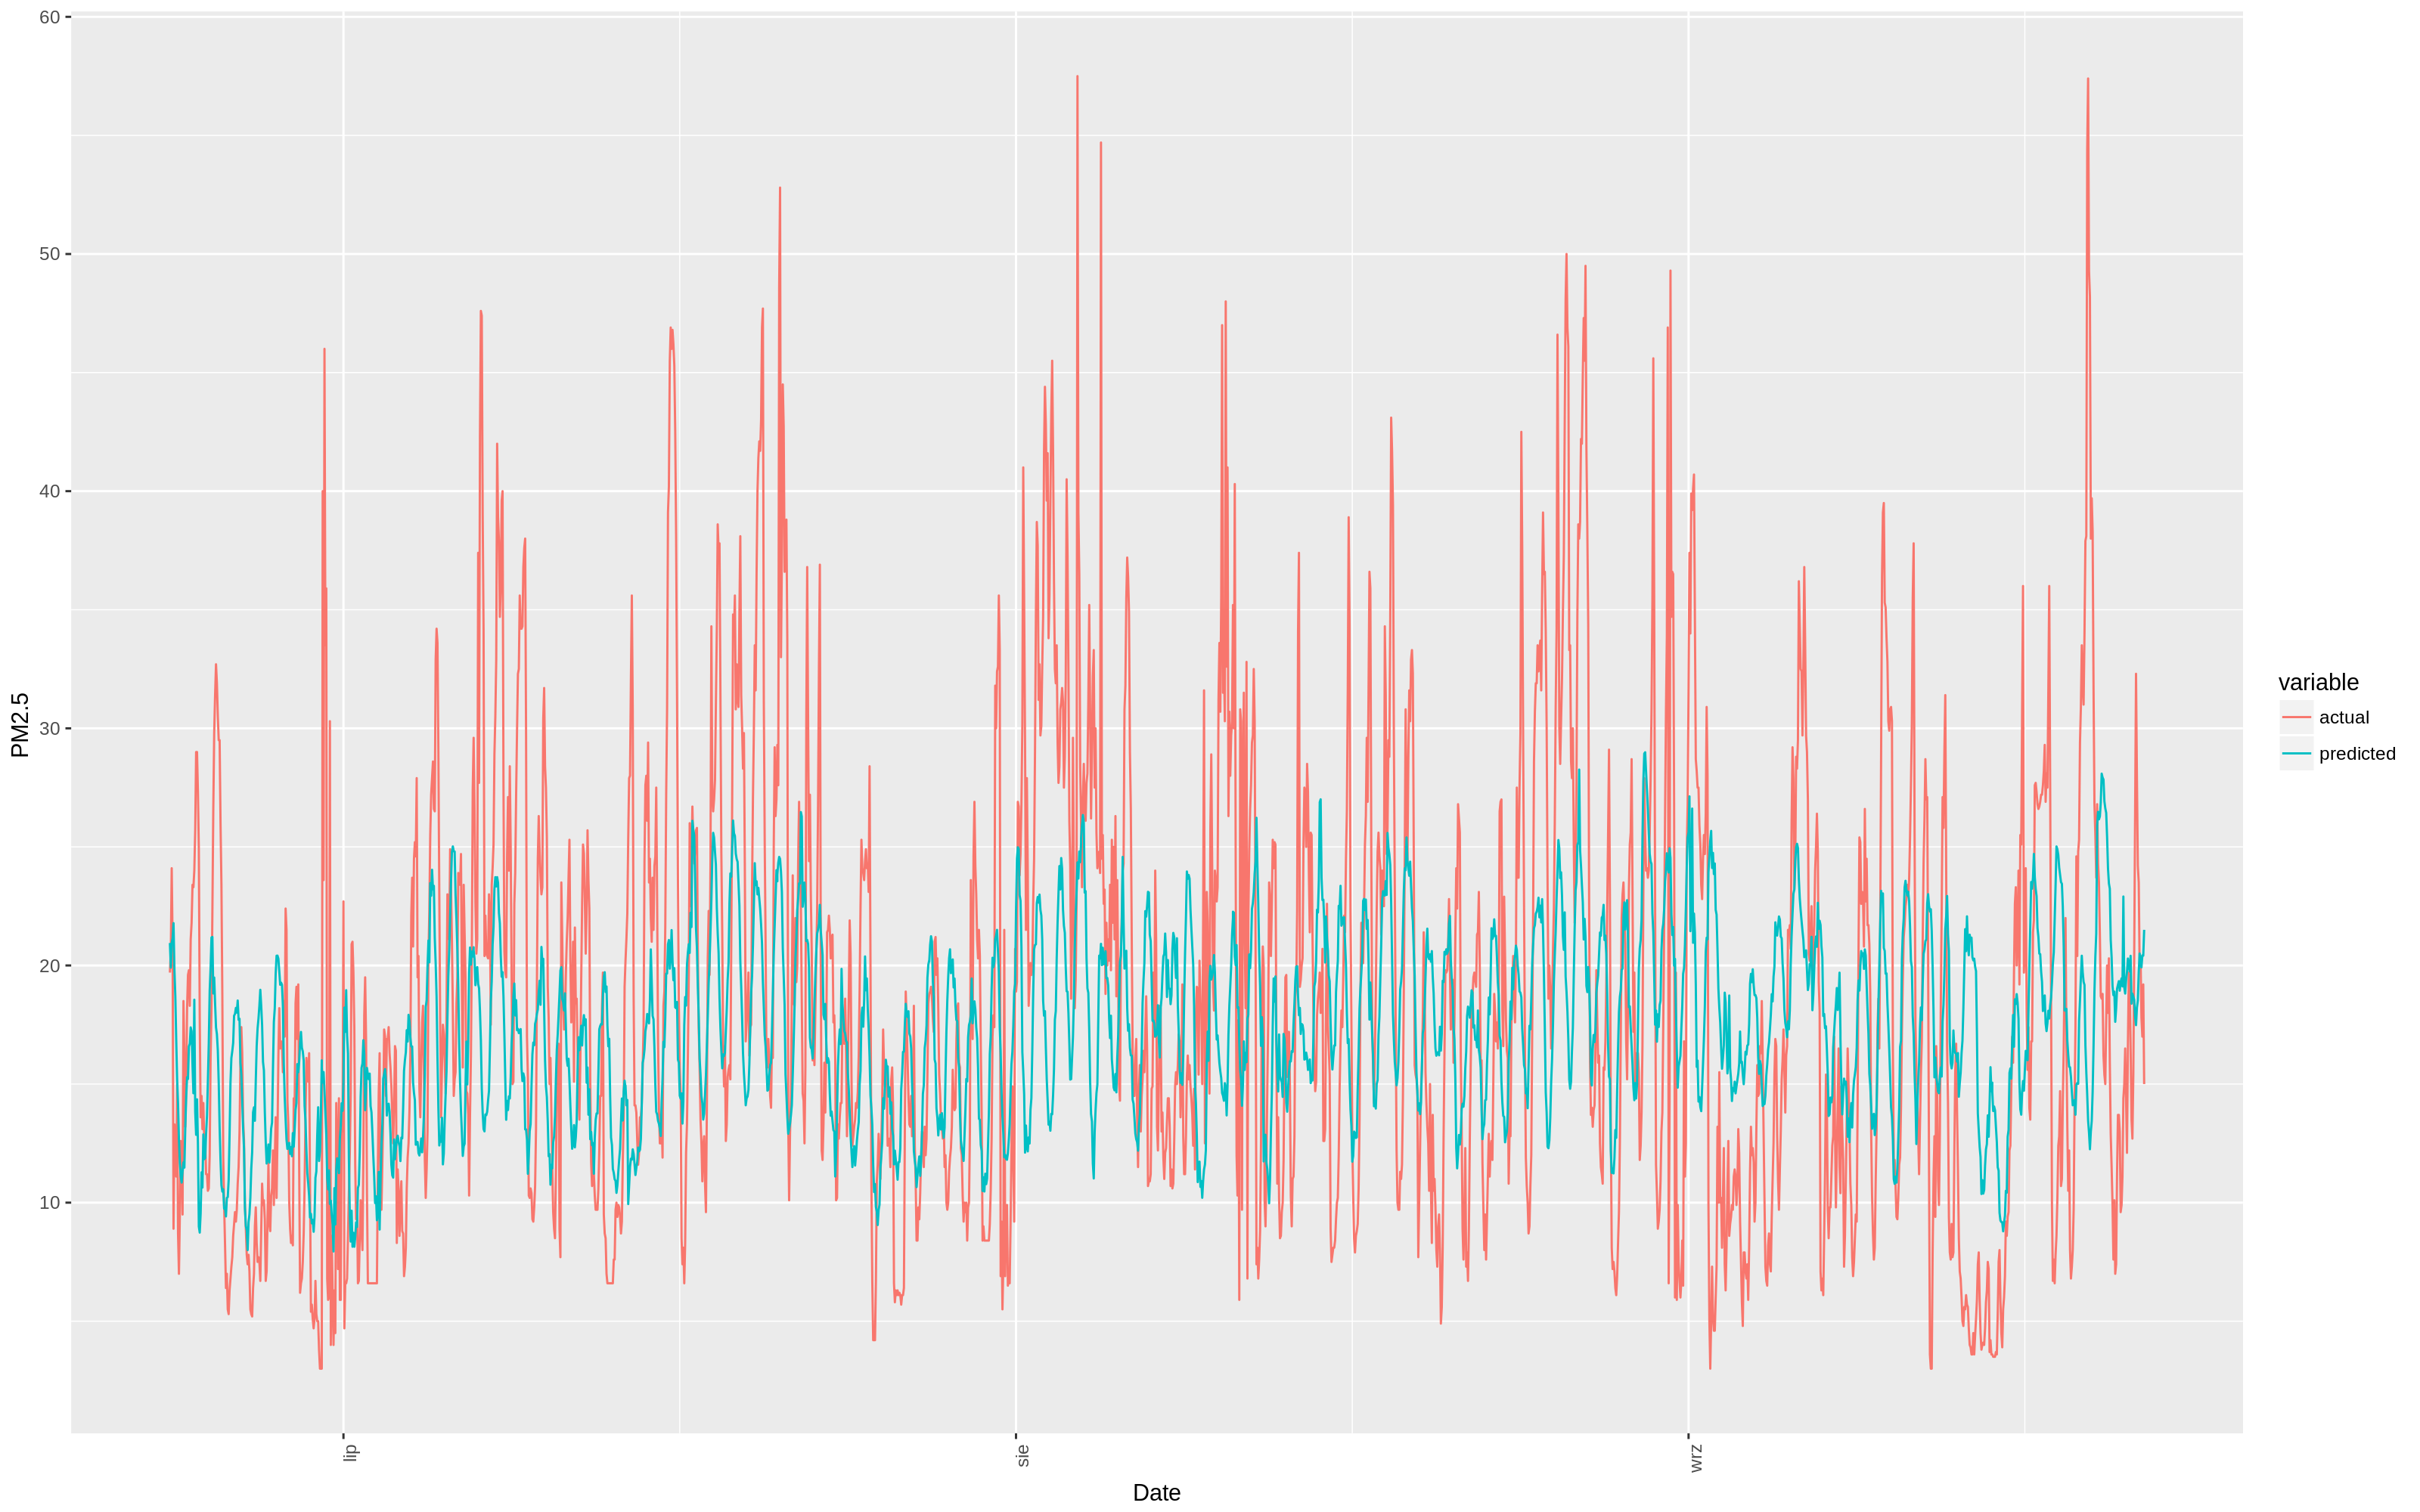
\includegraphics[width=\linewidth]{{figures/results/best-models/bujaka/all-data/summer/comparison_plot_log_mlr_lag_24}.png}
% \caption{Comparison of actual and predicted PM2.5 concentrations - GIOŚ Bujaka, summer, all data }
% \label{fig:results-comparison-bujaka-summer-all-data}
% \end{figure}
% \end{landscape}

% \begin{landscape}
% \begin{figure}[htp]
% \centering
% 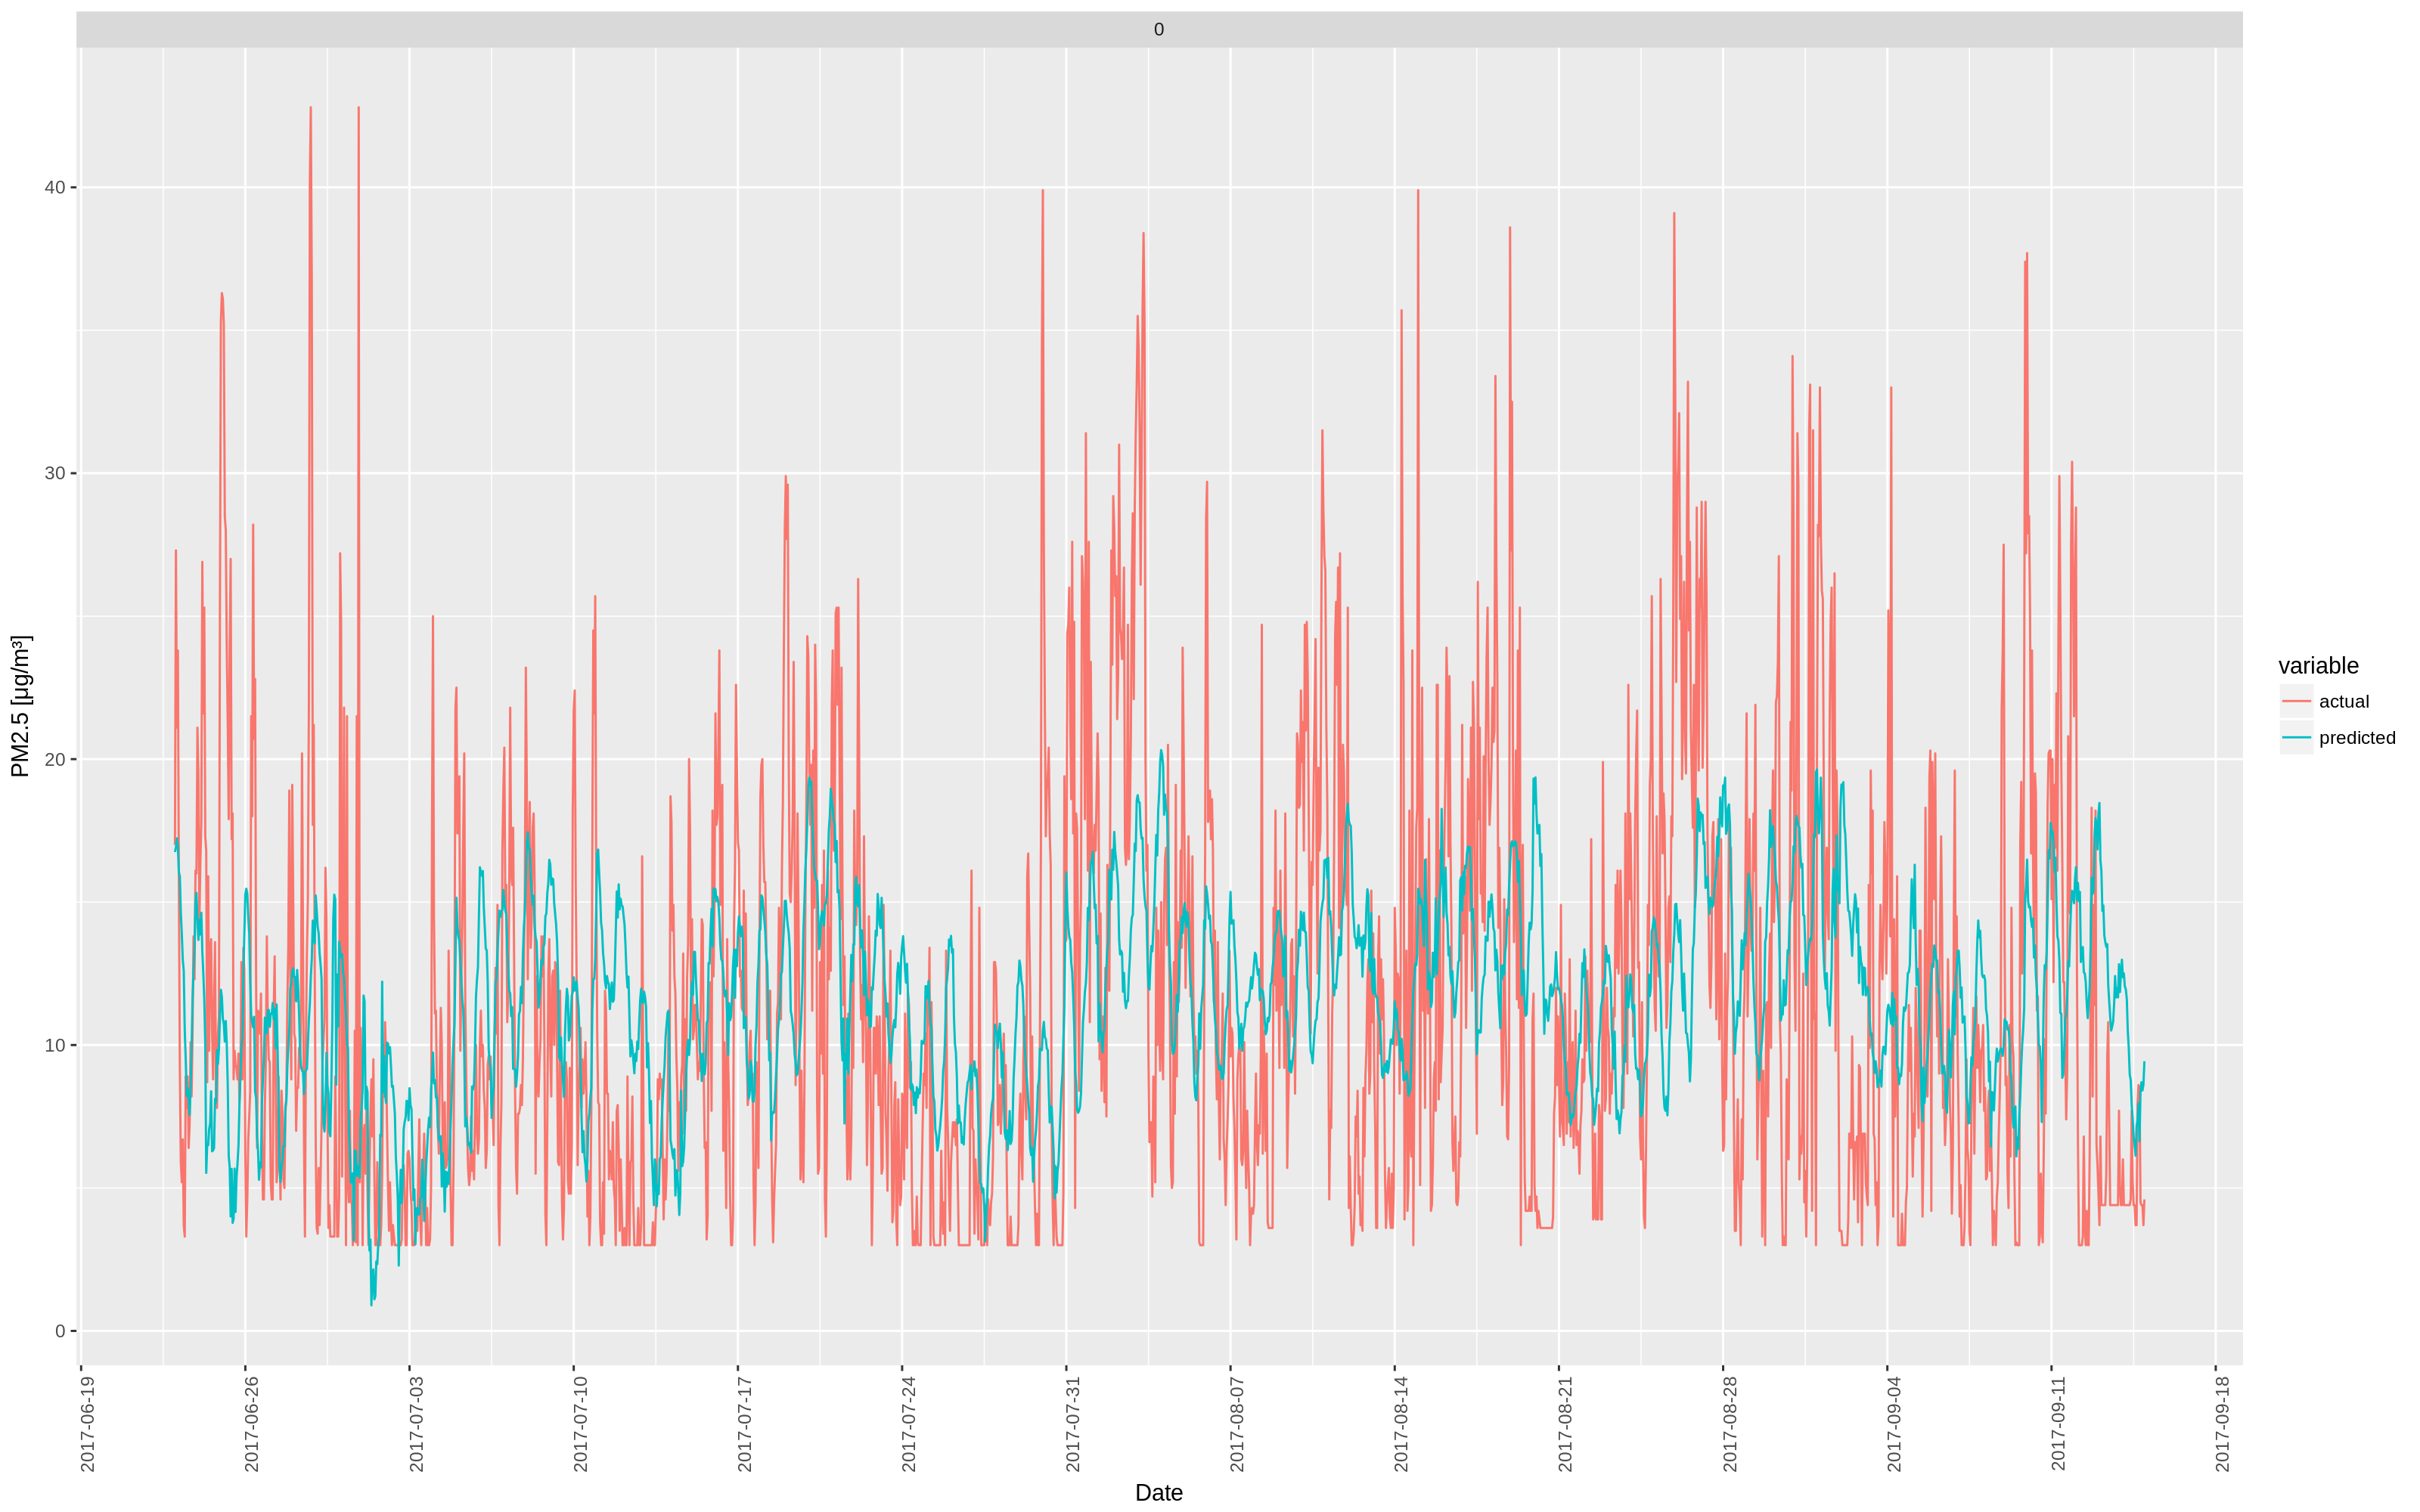
\includegraphics[width=\linewidth]{{figures/results/best-models/bujaka/same-season/summer/all_comparison_plot_svr_gam0.000244_eps0.5_c0.25_lag_24}.png}
% \caption{Comparison of actual and predicted PM2.5 concentrations - GIOŚ Bujaka, spring, same season }
% \label{fig:results-comparison-bujaka-summer-same-season}
% \end{figure}
% \end{landscape}

% \begin{landscape}
% \begin{figure}[htp]
% \centering
% 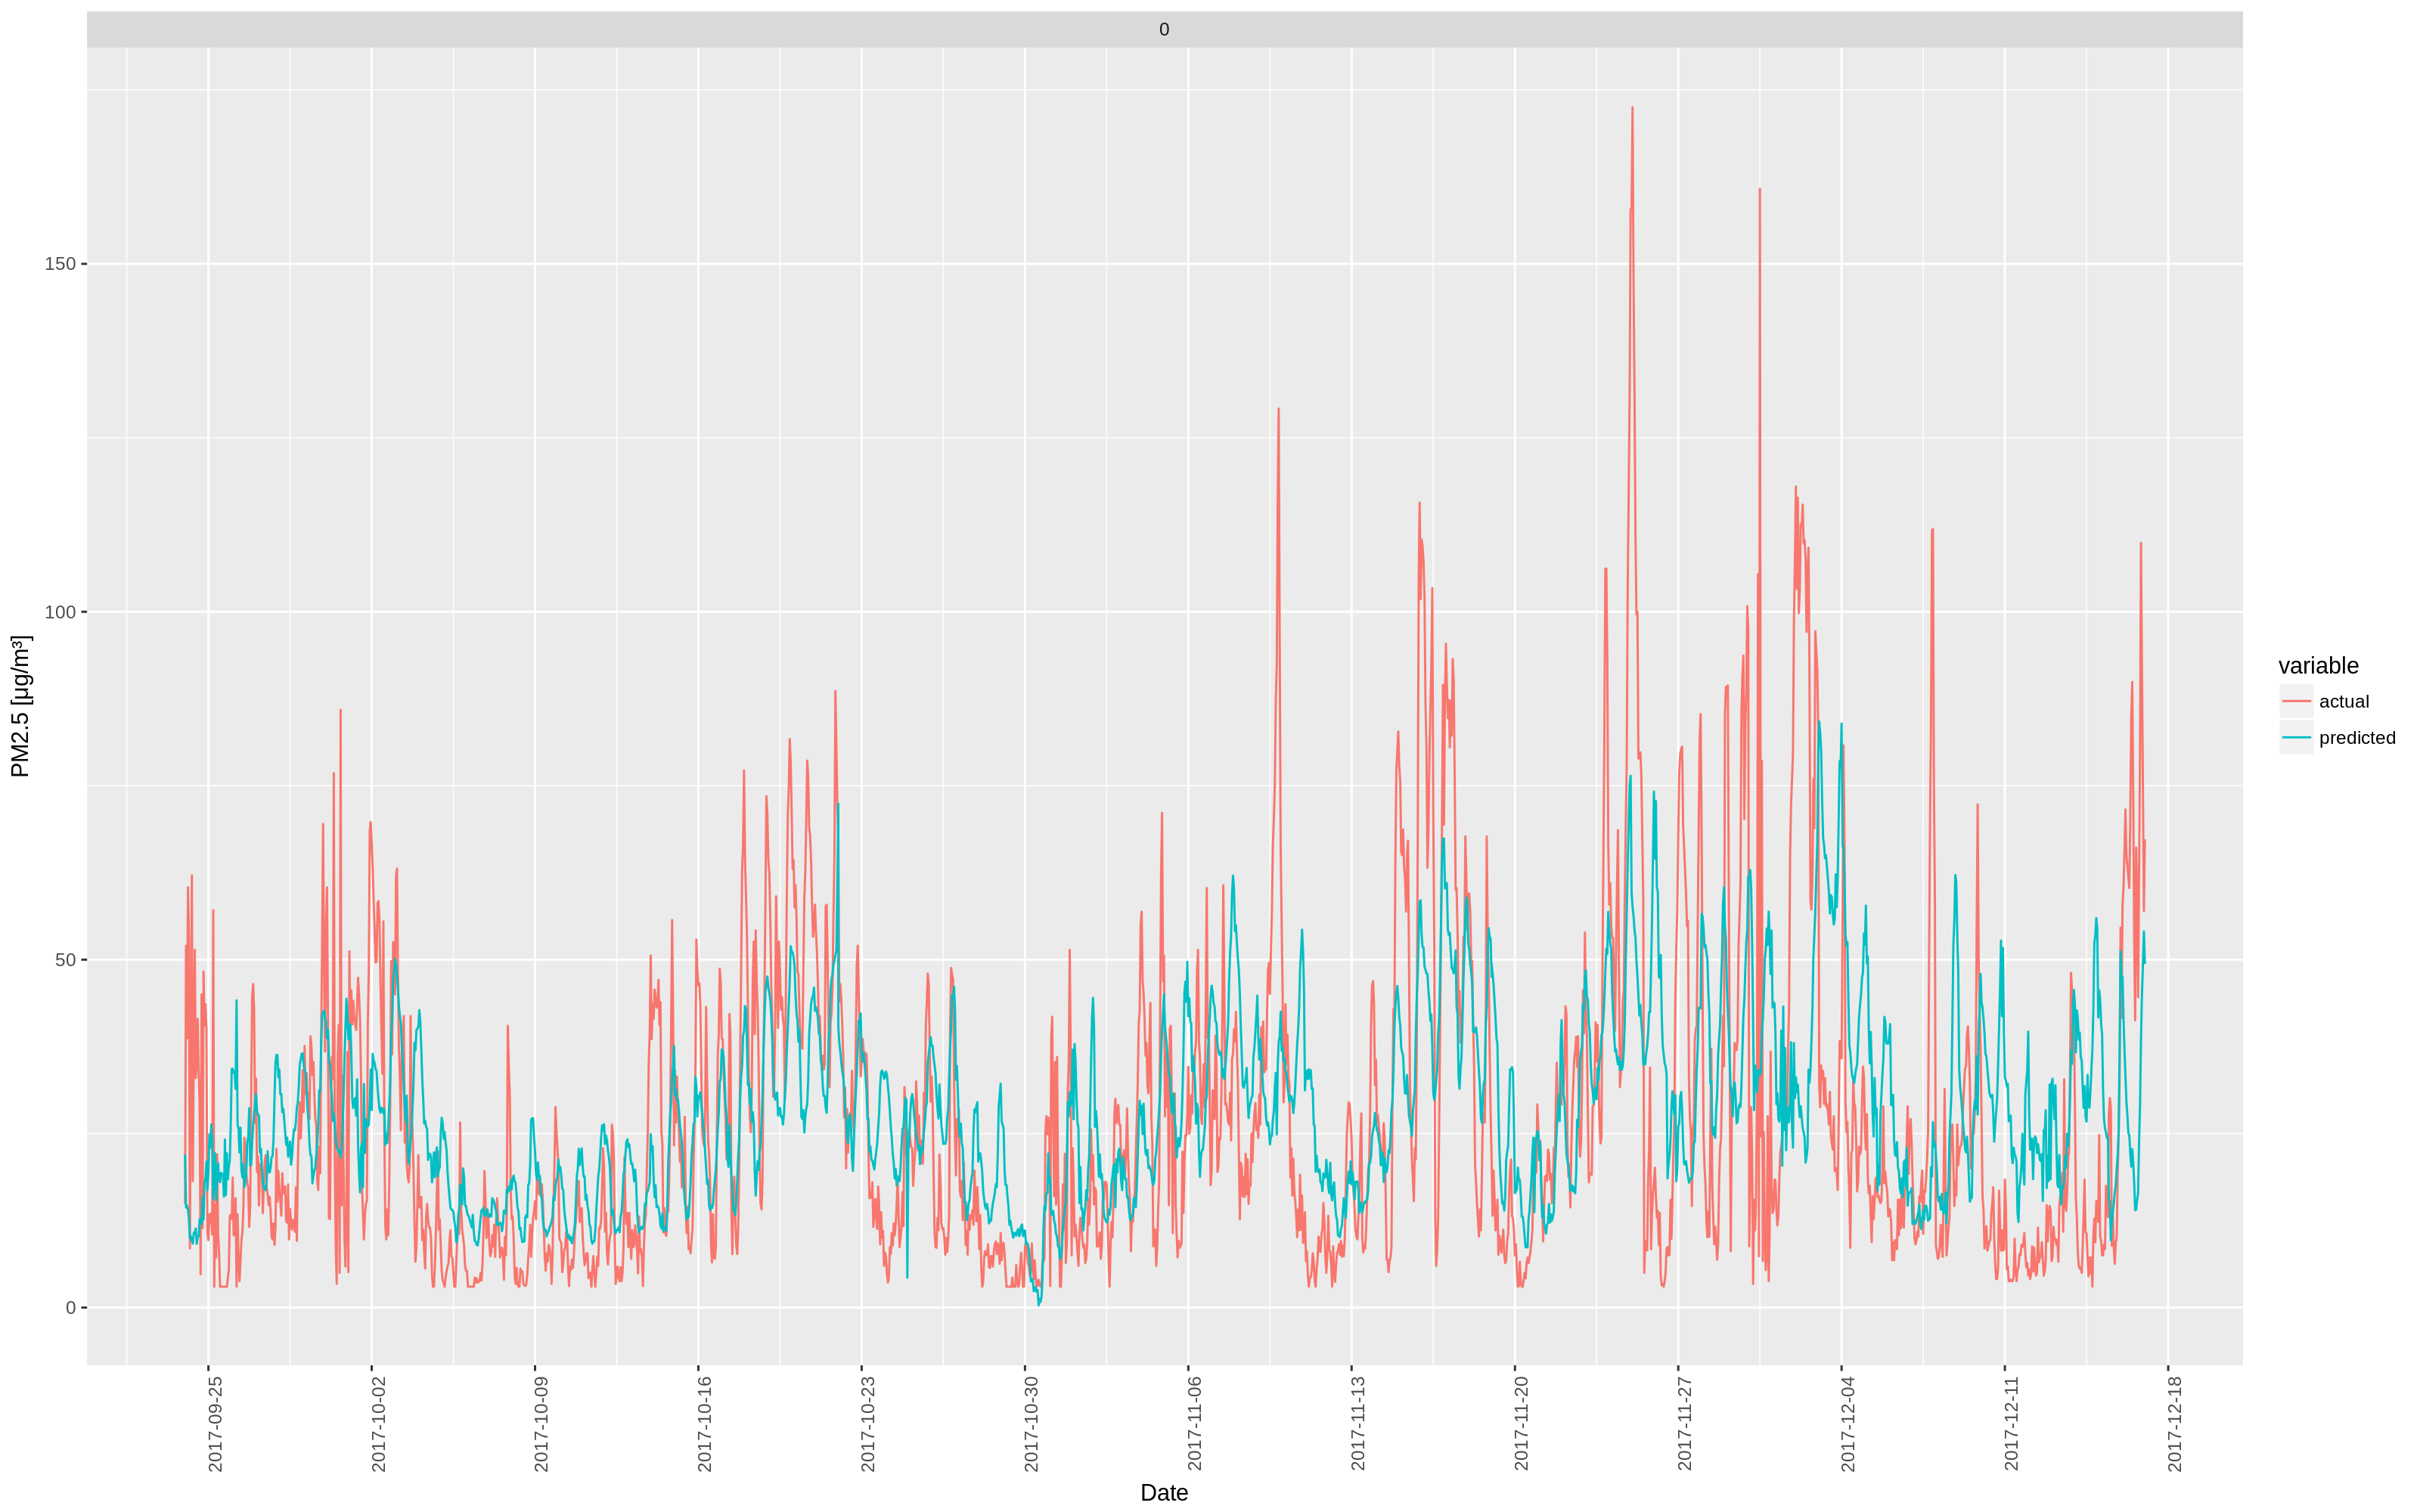
\includegraphics[width=\linewidth]{{figures/results/best-models/bujaka/all-data/autumn/comparison_plot_mlp5_5_5_th_0.5_lag_24}.png}
% \caption{Comparison of actual and predicted PM2.5 concentrations - GIOŚ Bujaka, autumn, all data }
% \label{fig:results-comparison-bujaka-autumn-all-data}
% \end{figure}
% \end{landscape}

% \begin{landscape}
% \begin{figure}[htp]
% \centering
% 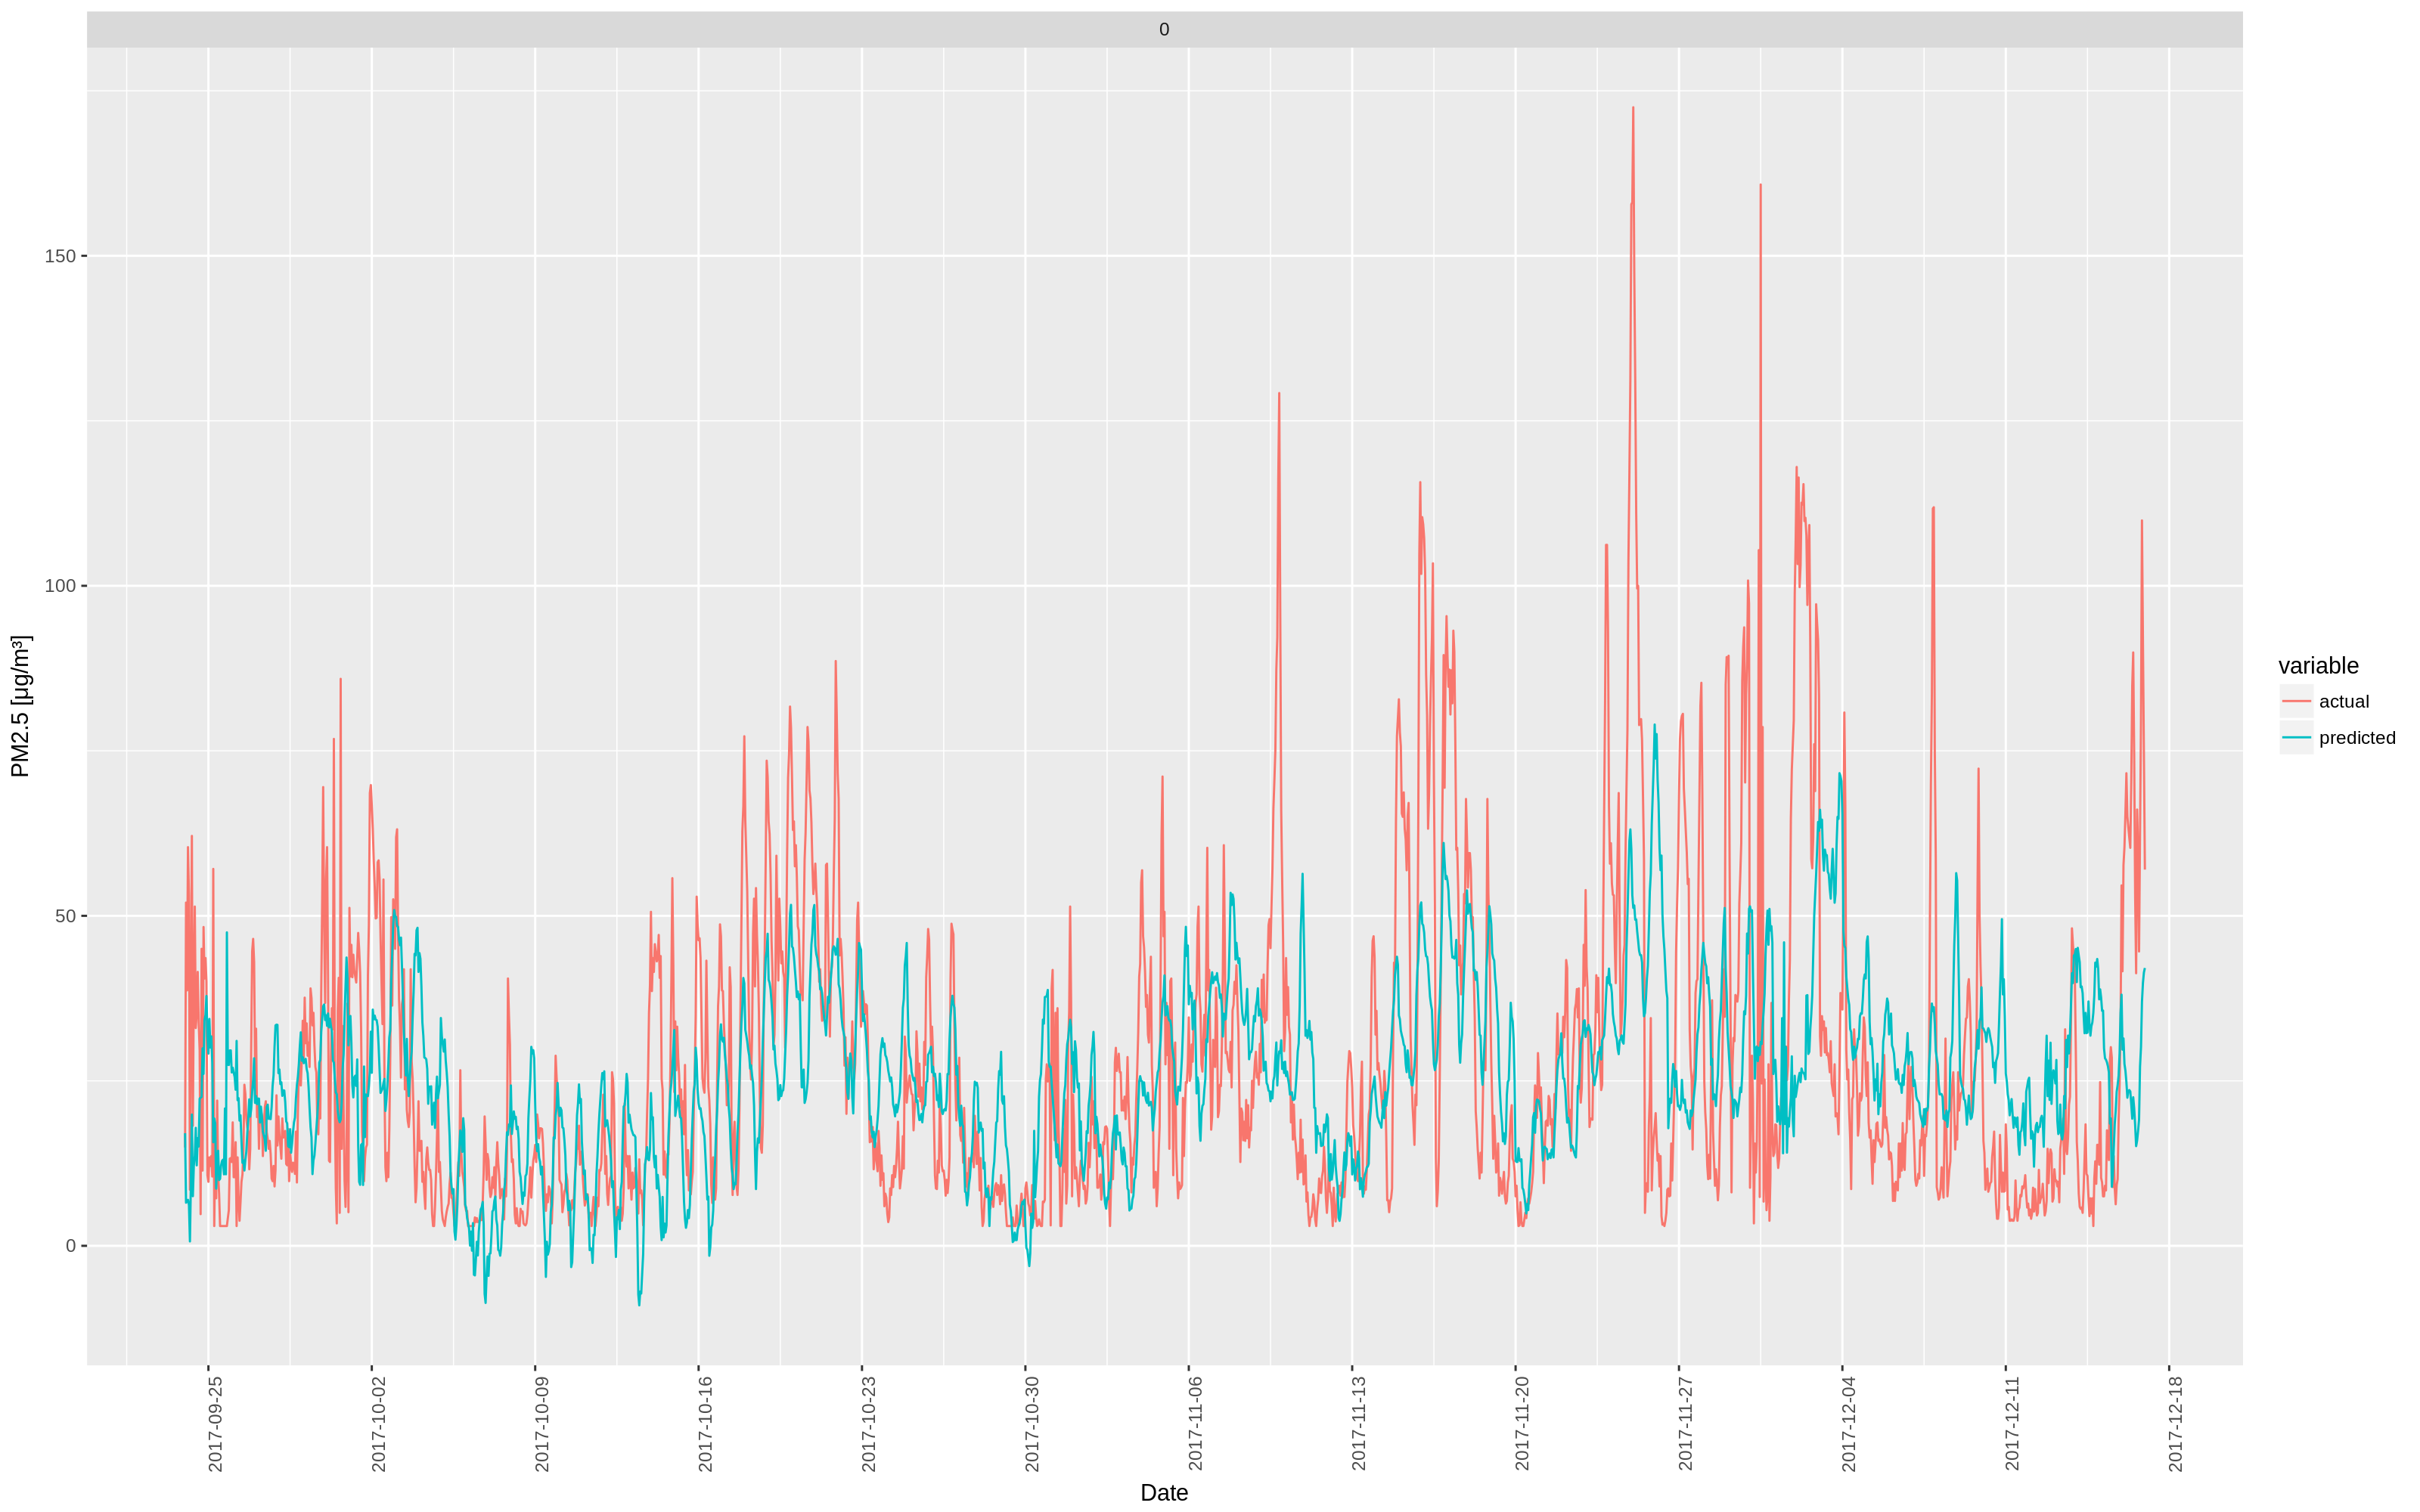
\includegraphics[width=\linewidth]{{figures/results/best-models/bujaka/same-season/autumn/all_comparison_plot_svr_gam0.000244_eps0.5_c16_lag_24}.png}
% \caption{Comparison of actual and predicted PM2.5 concentrations - GIOŚ Bujaka, autumn, same season }
% \label{fig:results-comparison-bujaka-autumn-same-season}
% \end{figure}
% \end{landscape}

% % GIOŚ Bulwarowa

% \begin{landscape}
% \begin{figure}[htp]
% \centering
% \includegraphics[width=\linewidth]{{figures/results/best-models/bulwarowa/all-data/winter/comparison_plot_mlr_lag_24}.png}
% \caption{Comparison of actual and predicted PM2.5 concentrations - GIOŚ Bulwarowa, winter, all data }
% \label{fig:results-comparison-bulwarowa-winter-all-data}
% \end{figure}
% \end{landscape}

% \begin{landscape}
% \begin{figure}[htp]
% \centering
% 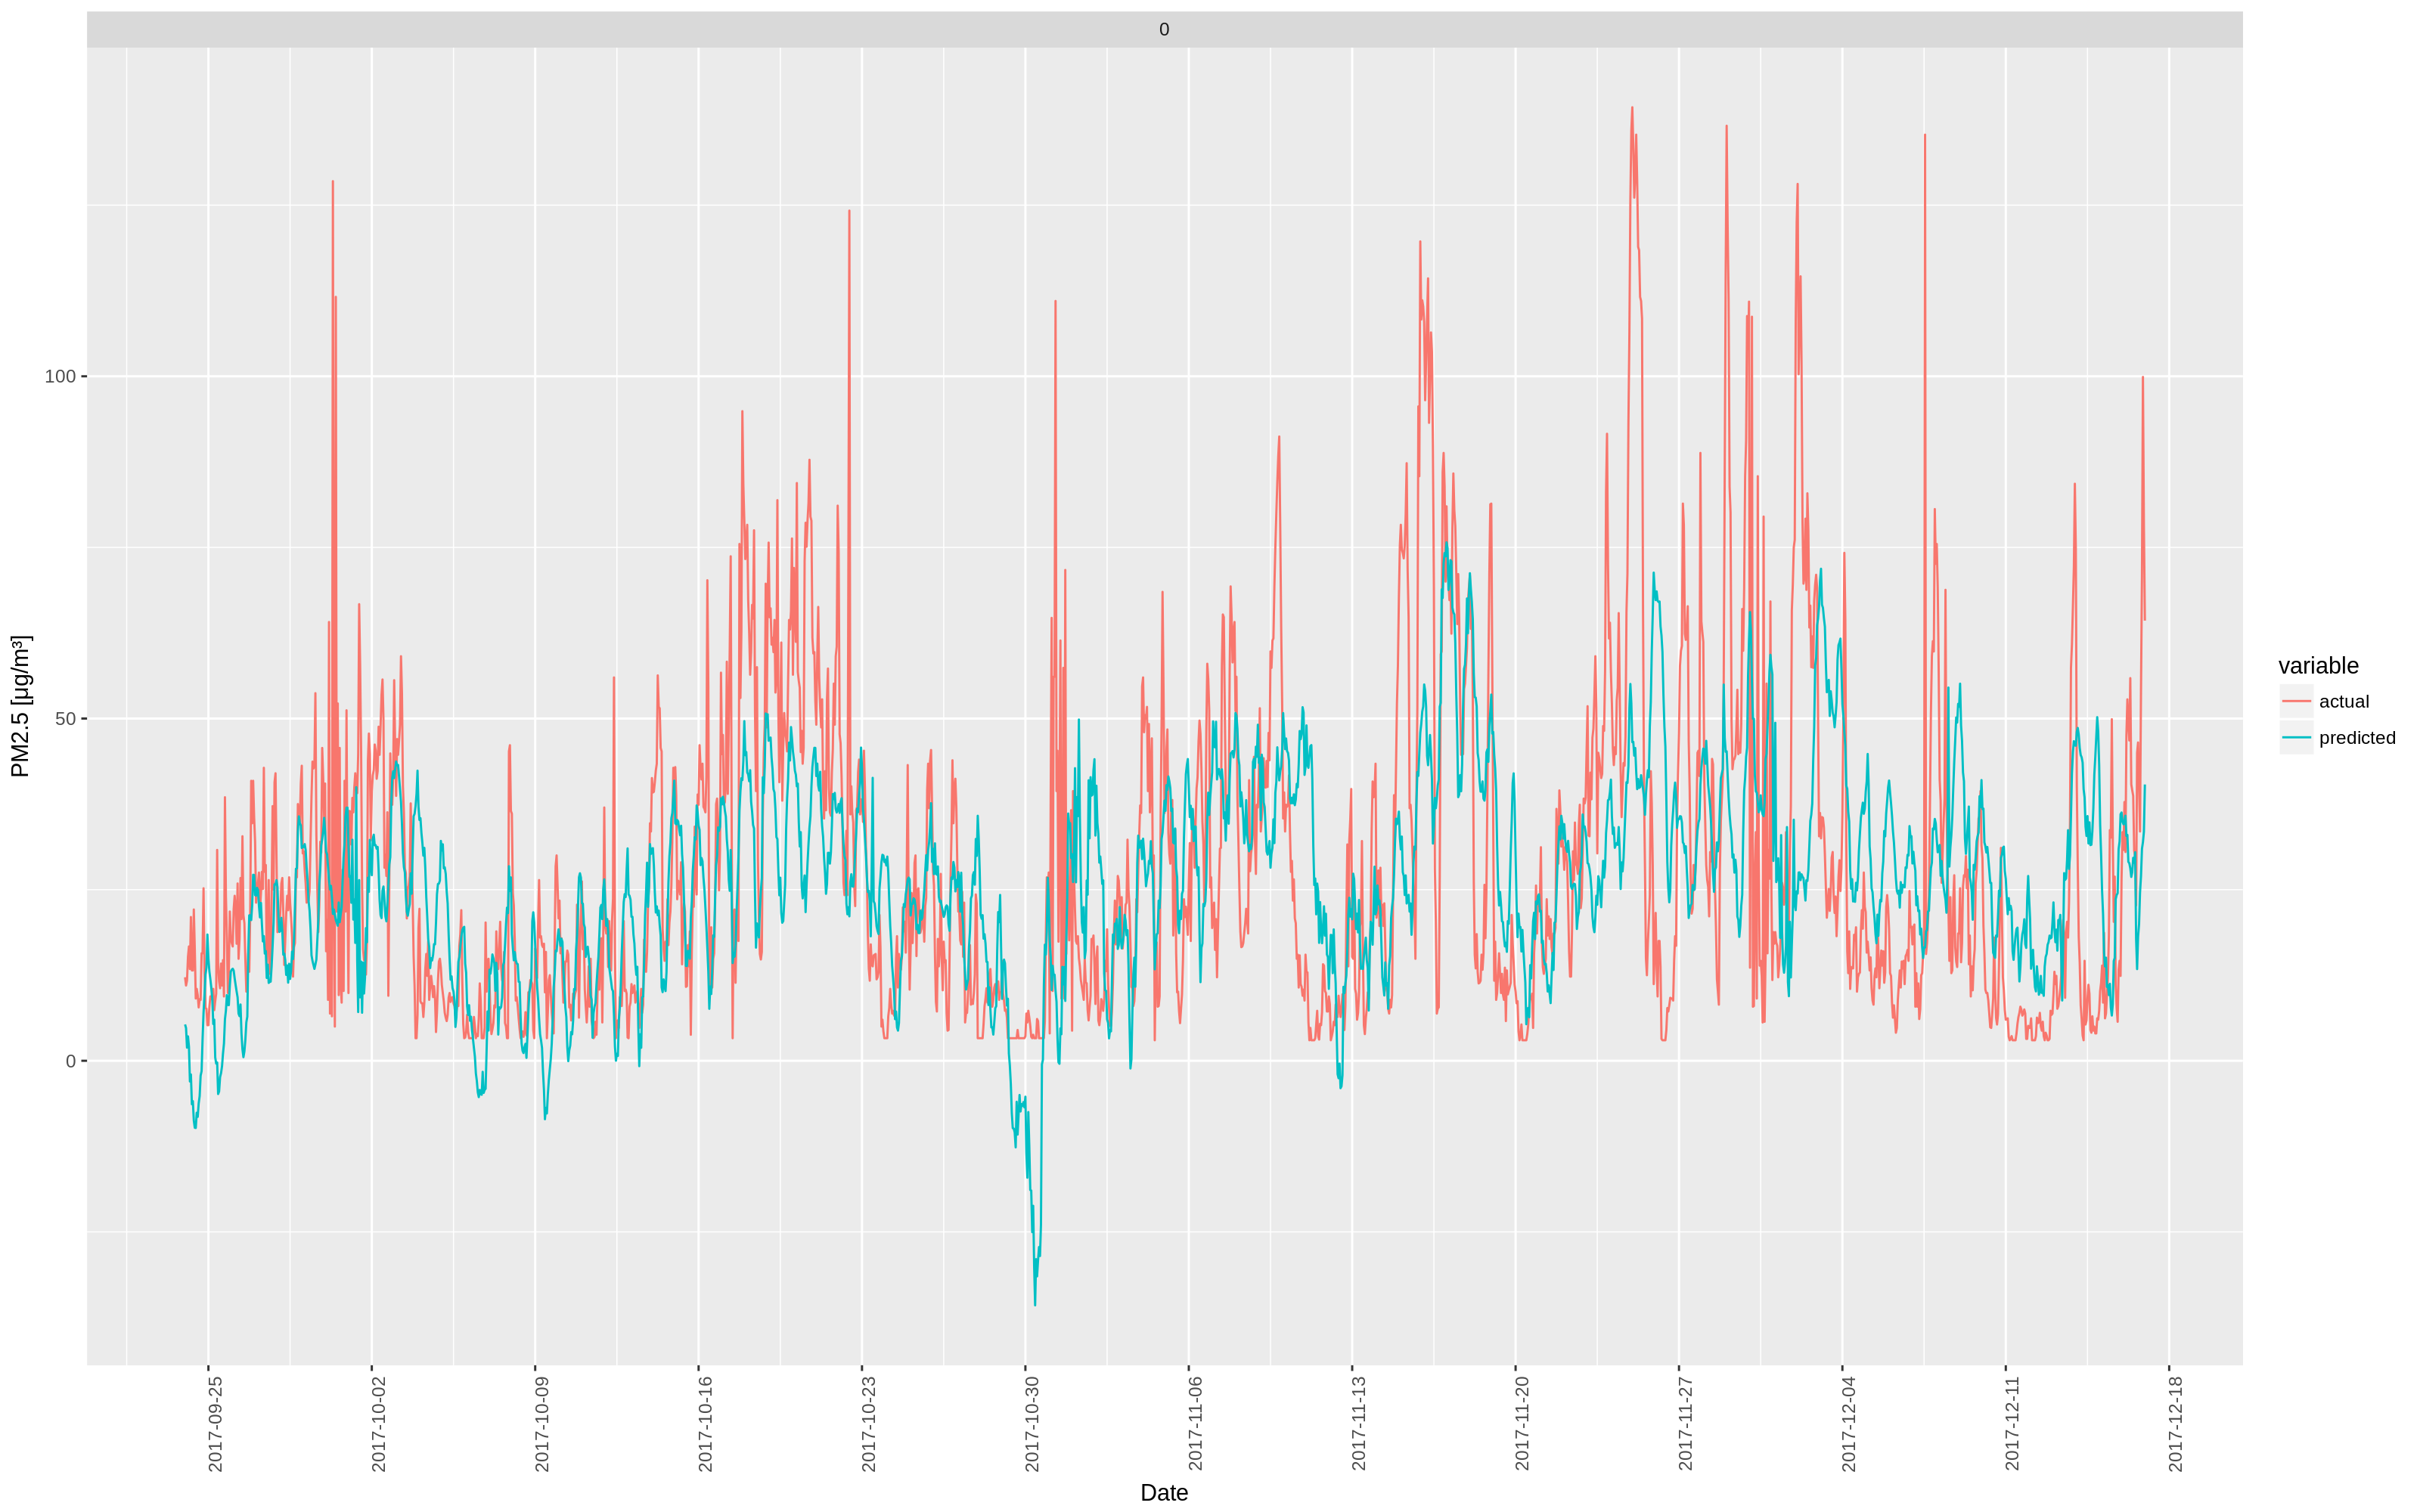
\includegraphics[width=\linewidth]{{figures/results/best-models/bulwarowa/same-season/winter/all_comparison_plot_lasso_mlr_lag_24}.png}
% \caption{Comparison of actual and predicted PM2.5 concentrations - GIOŚ Bulwarowa, winter, same season }
% \label{fig:results-comparison-bulwarowa-winter-same-season}
% \end{figure}
% \end{landscape}

% \begin{landscape}
% \begin{figure}[htp]
% \centering
% 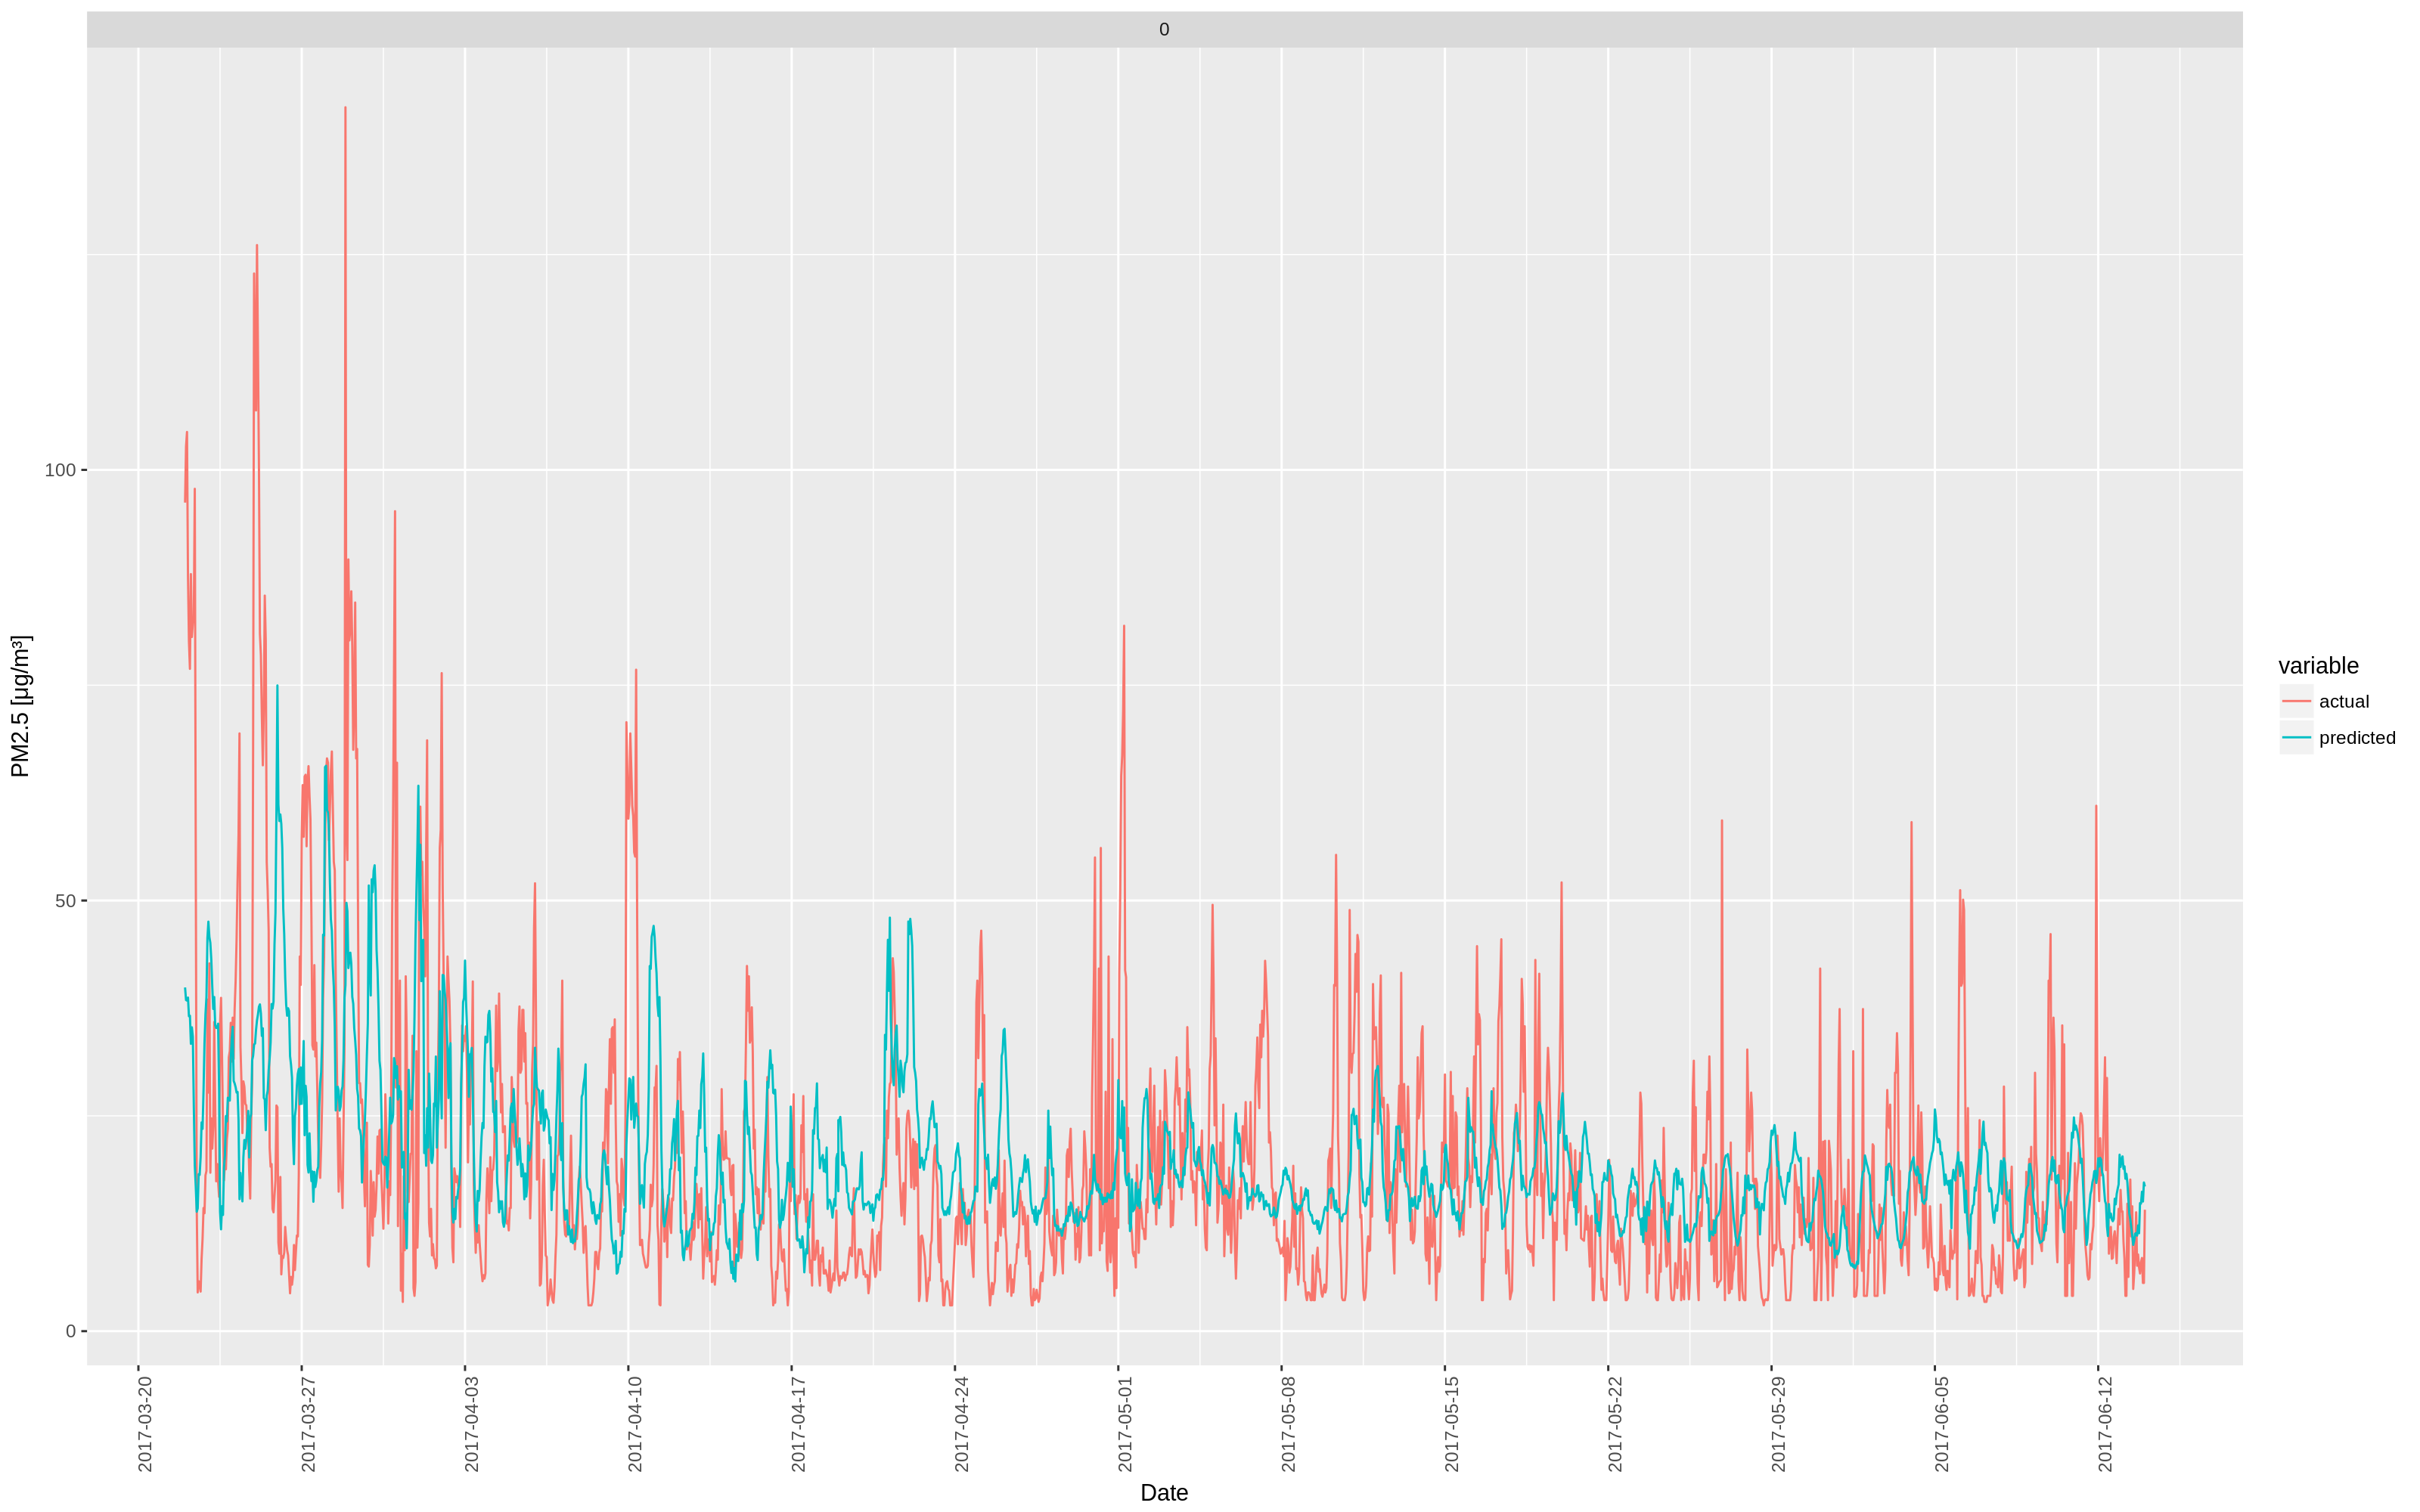
\includegraphics[width=\linewidth]{{figures/results/best-models/bulwarowa/all-data/spring/comparison_plot_mlp3_6_5_th_0.7_lag_24}.png}
% \caption{Comparison of actual and predicted PM2.5 concentrations - GIOŚ Bulwarowa, spring, all data }
% \label{fig:results-comparison-bulwarowa-spring-all-data}
% \end{figure}
% \end{landscape}

% \begin{landscape}
% \begin{figure}[htp]
% \centering
% \includegraphics[width=\linewidth]{{figures/results/best-models/bulwarowa/same-season/spring/all_comparison_plot_svr_gam0.000977_eps0.25_c0.25_lag_24}.png}
% \caption{Comparison of actual and predicted PM2.5 concentrations - GIOŚ Bulwarowa, spring, same season }
% \label{fig:results-comparison-bulwarowa-spring-same-season}
% \end{figure}
% \end{landscape}

% \begin{landscape}
% \begin{figure}[htp]
% \centering
% \includegraphics[width=\linewidth]{{figures/results/best-models/bulwarowa/all-data/summer/comparison_plot_svr_gam0.00391_eps0.0312_c0.25_lag_24}.png}
% \caption{Comparison of actual and predicted PM2.5 concentrations - GIOŚ Bulwarowa, summer, all data }
% \label{fig:results-comparison-bulwarowa-summer-all-data}
% \end{figure}
% \end{landscape}

% \begin{landscape}
% \begin{figure}[htp]
% \centering
% \includegraphics[width=\linewidth]{{figures/results/best-models/bulwarowa/same-season/summer/all_comparison_plot_svr_gam0.000977_eps0.25_c0.25_lag_24}.png}
% \caption{Comparison of actual and predicted PM2.5 concentrations - GIOŚ Bulwarowa, spring, same season }
% \label{fig:results-comparison-bulwarowa-summer-same-season}
% \end{figure}
% \end{landscape}

% \begin{landscape}
% \begin{figure}[htp]
% \centering
% \includegraphics[width=\linewidth]{figures/results/best-models/bulwarowa/all-data/autumn/{comparison_plot_svr_gam0_00391_eps0.0312_c0.25_lag_24}.png}
% \caption{Comparison of actual and predicted PM2.5 concentrations - GIOŚ Bulwarowa, autumn, all data}
% \label{fig:results-comparison-bulwarowa-autumn-all-data}
% \end{figure}
% \end{landscape}

% \begin{landscape}
% \begin{figure}[htp]
% \centering
% \includegraphics[width=\linewidth]{{figures/results/best-models/bulwarowa/same-season/autumn/all_comparison_plot_lasso_mlr_lag_24}.png}
% \caption{Comparison of actual and predicted PM2.5 concentrations - GIOŚ Bulwarowa, autumn, same season }
% \label{fig:results-comparison-bulwarowa-autumn-same-season}
% \end{figure}
% \end{landscape}

% % GIOŚ Krasińskiego
\begin{landscape}
\begin{figure}[ht]
\centering
\includegraphics[width=\linewidth]{{figures/results/best-models/krasinskiego/all-data/winter/comparison_plot_mlr_lag_24}.png}
\caption{Comparison of actual and predicted PM2.5 concentrations - GIOŚ Krasińskiego, winter, all data }
\label{fig:results-comparison-krasinskiego-winter-all-data}
\end{figure}
\end{landscape}

% \begin{landscape}
% \begin{figure}[htp]
% \centering
% \includegraphics[width=\linewidth]{{figures/results/best-models/krasinskiego/same-season/winter/all_comparison_plot_mlr_lag_24}.png}
% \caption{Comparison of actual and predicted PM2.5 concentrations - GIOŚ Krasińskiego, winter, same season }
% \label{fig:results-comparison-krasinskiego-winter-same-season}
% \end{figure}
% \end{landscape}

% \begin{landscape}
% \begin{figure}[htp]
% \centering
% \includegraphics[width=\linewidth]{{figures/results/best-models/krasinskiego/all-data/spring/comparison_plot_svr_gam0.000977_eps2_c1_lag_24}.png}
% \caption{Comparison of actual and predicted PM2.5 concentrations - GIOŚ Krasińskiego, spring, all data }
% \label{fig:results-comparison-krasinskiego-spring-all-data}
% \end{figure}
% \end{landscape}

% \begin{landscape}
% \begin{figure}[htp]
% \centering
% \includegraphics[width=\linewidth]{{figures/results/best-models/krasinskiego/same-season/spring/all_comparison_plot_svr_gam0.000977_eps0.25_c0.25_lag_24}.png}
% \caption{Comparison of actual and predicted PM2.5 concentrations - GIOŚ Krasińskiego, spring, same season }
% \label{fig:results-comparison-krasinskiego-spring-same-season}
% \end{figure}
% \end{landscape}

% \begin{landscape}
% \begin{figure}[htp]
% \centering
% \includegraphics[width=\linewidth]{{figures/results/best-models/krasinskiego/all-data/summer/comparison_plot_svr_gam0.00391_eps0.0312_c0.25_lag_24}.png}
% \caption{Comparison of actual and predicted PM2.5 concentrations - GIOŚ Krasińskiego, summer, all data }
% \label{fig:results-comparison-krasinskiego-summer-all-data}
% \end{figure}
% \end{landscape}

% \begin{landscape}
% \begin{figure}[htp]
% \centering
% \includegraphics[width=\linewidth]{{figures/results/best-models/krasinskiego/same-season/summer/all_comparison_plot_lasso3_lag_24}.png}
% \caption{Comparison of actual and predicted PM2.5 concentrations - GIOŚ Krasińskiego, spring, same season }
% \label{fig:results-comparison-krasinskiego-summer-same-season}
% \end{figure}
% \end{landscape}

% \begin{landscape}
% \begin{figure}[htp]
% \centering
% \includegraphics[width=\linewidth]{{figures/results/best-models/krasinskiego/all-data/autumn/comparison_plot_mlp2_5_5_th_0.5_lag_24}.png}
% \caption{Comparison of actual and predicted PM2.5 concentrations - GIOŚ Krasińskiego, autumn, all data }
% \label{fig:results-comparison-krasinskiego-autumn-all-data}
% \end{figure}
% \end{landscape}

% \begin{landscape}
% \begin{figure}[htp]
% \centering
% \includegraphics[width=\linewidth]{{figures/results/best-models/krasinskiego/same-season/autumn/all_comparison_plot_mlp4_3_2_th_0.3_lag_24}.png}
% \caption{Comparison of actual and predicted PM2.5 concentrations - GIOŚ Krasińskiego, autumn, same season }
% \label{fig:results-comparison-krasinskiego-autumn-same-season}
% \end{figure}
% \end{landscape}

\chapter{Conclusions and future works} \label{chap:conclusions}

\section{Achieved goals and observations}

\bt 

\section{Areas for development}

\bt



\chapter*{Acknowledgements}
This research was supported in part by PLGrid Infrastructure.

\cleardoublepage % to ensure that the page reference is correct
\addcontentsline{toc}{chapter}{\listfigurename}
\listoffigures

% \nocite{*}
% forces bibtex to include all citations, whether or not they were referred to in the paper

\cleardoublepage
\addcontentsline{toc}{chapter}{Bibliography}
\bibliographystyle{apalike}
\bibliography{bibliography}

\end{document}

